\documentclass{umnStatThesis}
%\documentclass{umnStatThesis}
\usepackage{mycommands1,color,caption,hyperref,amsmath,amssymb,amsthm,mathabx}
%\usepackage[pdftex]{graphicx}
\usepackage{subfigure,epsfig}
\usepackage{outlines}
%\usepackage{quotchap}

% use type-1 fonts
\usepackage[T1]{fontenc}
\usepackage{lmodern}
%\usepackage{times}
\pdfminorversion=4              % tell pdflatex to generate PDF in version 1.4
%\usepackage{ae,aecompl}

\author{Subhabrata Majumdar}
\adviser{Snigdhansu Chatterjee}
%\coadviser{Co-Adviser Name Here}
\title{An Inferential Perspective on Data Depth}
\month{May}
\year{2017}
% Month and Year of Degree Clearance, NOT necessarily when you defended

\begin{document}

\newtheorem{Theorem}{Theorem}[section]
\newtheorem{Lemma}[Theorem]{Lemma}
\newtheorem{Corollary}[Theorem]{Corollary}
\newtheorem{Proposition}[Theorem]{Proposition}
\newtheorem{Conjecture}[Theorem]{Conjecture}
\theoremstyle{definition} \newtheorem{Definition}[Theorem]{Definition}
\theoremstyle{definition} \newtheorem{Example}[Theorem]{Example}

%\makesignaturepage % required
\maketitlepage % required
%\makecopyrightpage % recommended, required if registering copyright

%% Copyright page
\begin{prepage}

\begin{minipage}{.7\textwidth}
\vspace{2em}
\begin{flushleft}
{\it
Truth is ever to be found in simplicity, and not in the multiplicity and confusion of things.}
\end{flushleft}

\begin{flushright}
- Issac Newton \hspace{3em}
\end{flushright}

\begin{flushleft}
{\it
Simplicity is the final achievement. After one has played a vast quantity of notes and more notes, it is simplicity that emerges as the crowning reward of art.}
\end{flushleft}

\begin{flushright}
- Fr\'ed\'eric Chopin
\end{flushright}
\end{minipage}


\vspace*{\fill}
\copyright\ Subhabrata Majumdar 2017
\end{prepage}

\frontmatter

\begin{acknowledgementspage} % optional
I would like to thank my advisor, Prof. Snigdhansu Chatterjee for everything he has done for me. This dissertation would not have been possible without the very fundamental ideas behind it that came out of our discussions during the first two years of my PhD. Anshu da gave me the freedom to pursue those ideas and shape them as I wanted. I am thankful for the professional support he provided, as well as for always being available to listen to my ramblings. I am going to miss those weekly meetings in which we talked about anything and everything statistics.

I want to thank Prof. Saonli Basu of the Division of Biostatistics, with whom I collaborated during my last year. She has been an invaluable mentor, and discussions with her helped me learn about many applied aspects of the problems we had worked on. Thanks to her for being a reviewer of this dissertation as well. Special thanks to Profs. Lan Wang and Xiaotong Shen for reviewing the thesis and being on the final exam committee, and Prof. Gongjun Xu for being in my oral committee.

I would like to thank other professors in the department, who have always been helpful in answering questions, and the staff in the department office for their support regarding official matters. Thanks to other students in the department, for being there with feedback and discussions: especially Abhirup, Adam, Aaron, Daniel, Dootika and Sakshi.

I would like to acknowledge the National Science Foundation Climate Expeditions grant IIS-1029711, which provided me funding for 3 semesters, and the University of Minnesota Graduate School's Interdisciplinary Doctoral Fellowship (IDF), which supported me during my final year.

I consider myself very fortunate to have worked with a number of collaborators while still being a graduate student. Thanks to Profs. Matt McGue and Mike Miller of the Department of Psychology for their help during the IDF collaboration. Outside the campus, I am grateful to Prof. Subhash C. Basak of University of Minnesota Duluth for helping me write my first paper back in 2012 and all subsequent collaborations. Rayid Ghani of University of Chicago and Kush Varshney of IBM Research have been inspirations in developing my approach to collaborative research.

Coming to personal life, I would like to thank my friends for keeping me grounded and connected to the world outside. Special thanks to the three musketeers- Abhirup Mallik, Somnath Kundu and Suvankar Biswas, for being part of many happy memories during the past five years. I am grateful to Abhishek Nandy, for all his support during my first two years. Thanks to Amit da, Arja, Deepashree, Shriya, Tallin di, Taraswi di, Tushar and many more people associated with the Bengali Student Society of Minnesota, life in Minneapolis has been so much enjoyable.

I would like to thank my teachers from school, Prabhat Kusum Sarkar for introducing me to statistics, and Tapas Kumar Dhar for helping me build the necessary mathematical foundation. The past five years would not have been possible without the all-encompassing influence of Indian Statistical Institute (ISI), where I finished my bachelors and masters degree. This is too short a space to list all the avenues the ISI connection has helped me through in terms of personal and professional networking. I am thankful for being part of this ISI family.

Finally, I want to thank the people closest to me, my parents, for always being there no matter what. To them I owe more than anyone else in this world. In spite of coming from humble beginnings, they have the highest respect for the intellectual pursuit, and there is no substitute for the sacrifices they made in bringing me up. Ma and Baba, I dedicate this thesis to you.
\end{acknowledgementspage}

\begin{dedicationpage} % optional
This dissertation is dedicated to my parents:

\vspace{1em}
\noindent \textit{Samita Mazumder, my mother}- for being patient while teaching a little boy the alphabets of mathematics, and instilling in me the value of hard work; and

\vspace{1em}
\noindent \textit{Satyabrota Mazumder, my father}- for the many life lessons, and wholeheartedly supporting me in every major decision I have made.

\end{dedicationpage}

\begin{abstract} % optional
Data depth provides a plausible extension of robust univariate quantities like ranks, order statistics and quantiles in multivariate setup. Although depth has gained visibility and has seen many applications in recent years, especially in classification problems for multivariate and functional data, its generalizability and utility in achieving traditional parametric inferential goals is largely unexplored. In this thesis we develop several approaches to address this. In particular, firstly we define an evaluation map function that is more general than data depth, and establish several results in a parametric modelling context using a broad definition of a statistical model. A fast algorithm for covariate selection using data depths as evaluation functions arises as a special case of this. We demonstrate applications of this framework on data from diverse fields: namely climate science, medical imaging and behavioral genetics. Secondly we propose a multivariate rank transformation using data depth and use them for robust inference in location and scale problems in elliptical distributions. Thirdly, we lay out a depth-based regularization framework in multi-response regression, and derive a new method of nonconvex penalized sparse regression in the multitask situation. Across the thesis, several simulation studies and real data examples demonstrate the effectiveness of the methods developed here.
\end{abstract}

\tableofcontents % required
% required if you have any tables:
\cleardoublepage
\addcontentsline{toc}{chapter}{List of Tables}
\listoftables
% required if you have any figures:
\cleardoublepage
\addcontentsline{toc}{chapter}{List of Figures} 
\listoffigures
% Thanks to Lisa Lendway for noticing that the list of tables and figures needed to added to the table of contents.

\addcontentsline{toc}{chapter}{List of Notations} 
\chapter*{List of notations}

%\vspace{2em}
\begin{table}[h]
\centering
\begin{tabular}{cp{5in}}
\hline
Notation & Meaning \\\hline
$\BE$ & Expectation of a random variable (scalar/ vector/ matrix valued)\\
$\BV$ & Variance of a scalar-valued random variable or covariance matrix of a vector-valued random variable\\
$\BP$ & Probability of some event\\
$\leadsto$ & Convergence in distribution\\
$a_n \asymp b_n$ & $a_n = O(b_n)$ and $b_n = O(a_n)$ \\
$\|.\|$ & Euclidean norm for vectors, Frobenius norm for matrices, unless otherwise stated\\
$a_n  = O_{P_n} (b_n)$ & $a_n/b_n$ converges to some $c \in \BR$ in probability conditional on the data as $n \raro \infty$ \\
$a_n  = o_{P_n} (b_n)$ & $a_n/b_n$ converges to some $0$ in probability conditional on the data as $n \raro \infty$ \\$a_n  \stackrel{P_n}{\raro} b_n$ & $a_n$ converges to $b_n$ in probability conditional on the data as $n \raro \infty$ \\\hline 
\end{tabular}
\end{table}

\mainmatter

%% Introduction chapter
\chapter{Introduction}
\label{chapter:chapter-intro}

\section{Background}

The nonparametric concept of data depth had first been proposed by \cite{tukey75} when he introduced the halfspace depth. The motivation behind this was to formulate a unified framework for nonparametric inference in multivariate concept: in particular, the multivariate equivalent of methods based on signs and ranks, order statistics, quantiles and outlyingness functions. 

Given a dataset, the depth of a given point in the sample space measures how far inside the data cloud the point exists, i.e. it is a measure of centrality of the point with respect to the data. An overview of statistical depth functions can be found in \cite{zuo00}. Depth-based methods have gained popularity in the past two decades, for robust nonparametric classification \citep{jornsten04, ghosh05, dutta12, sguera14}. In parametric estimation, depth-weighted means \citep{ZuoCuiHe04} and covariance matrices \citep{ZuoCui05} provide high-breakdown point as well as efficient estimators, although they do involve choice of a suitable weight function and tuning parameters. As \cite{LiuSingh97} have shown, it is also possible to use statistical depth functions in hypothesis testing and an alternate notion of $p$-values. Approaching data depth as from the perspective of breakdown points, \cite{RousseeuwHubert99} also introduced the concept of regression depth, which was later generalized by \cite{Mizera02}.

\section{Definition and examples}
For any multivariate distribution $F$ taking values $\tilde \BR^p$ (or a subset of it), the depth of a point $\bfx \in \mathbb{R}^p$, say $D(\bfx, F_\bfX)$ is any real-valued function that provides a `center outward ordering' of $\bfx$ with respect to $F$ \citep{zuo00}. \ref{fig:depthplot} gives an intuition of data depth for samples from a bivariate normal distribution. As demonstrated by the contours and plot of values, a point close to the center, which coincides with the mean for elliptical distributions, has high depth. In other words, the point is situated deep inside the data/ underlying distribution. In comparison, a point closer to the periphery shall have less depth.

\begin{figure}
	\centering
		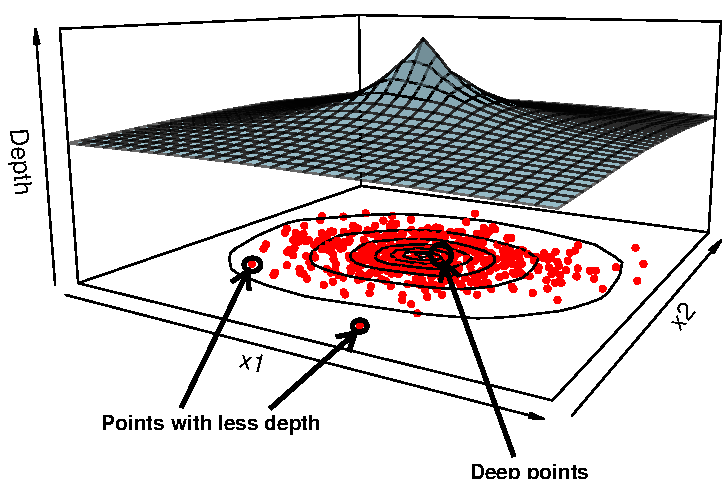
\includegraphics[width=7cm]{Chapter-regression/depthplot_cropped}
	\caption{Depth is a scalar measure of how much inside a point is with respect to a data cloud: 500 points from $\cN_2 ((0,0)^T, \diag (2,1))$}
	\label{fig:depthplot}
\end{figure}

In order to standardizing this notion \cite{liu90} outlined the desirable properties of a statistical depth function:

\vspace{1em}
\noindent\textbf{(P1)} \textit{Affine invariance}: $D(A\bfx + \bfb, \bfA F + \bfb) = D(\bfx, F)$ for any $\bfA\ \in \BR^{p \times p}, \bfb \in \BR^p$. Here $\bfA F + \bfb$ is a slight abuse of notation, and denotes the distribution of $\bfA \bfX + \bfb$ where $\bfX \sim F$;

\noindent\textbf{(P2)} \textit{Maximality at center}: $D(\bftheta, F) = \sup_{\bfx\in \mathbb{R}^p} D(\bfx, F)$ for $F$ having center of symmetry $\bftheta$. This point is called the \textit{deepest point} of the distribution.;

\noindent\textbf{(P3)} \textit{Decreasing from deepest point along any ray}: $D(\bfx; F) \leq D(\bftheta + a(\bfx - \bftheta), F)$;

\noindent\textbf{(P4)} \textit{Vanishing at infinity}: $D(\bfx; F) \rightarrow 0$ as $\|\bfx\| \rightarrow \infty $.

\vspace{1em}
In (P2) the types of symmetry considered can be central symmetry, angular symmetry and halfspace symmetry. Also for multimodal probability distributions, i.e. distributions with multiple local maxima in their probability density functions, properties (P2) and (P3) are actually restrictive towards the formulation of a reasonable depth function that captures the shape of the data cloud. Finally we think affine invariance is an artifact of depth functions being formulated keeping robustness with respect to elliptical distributions in mind, and in most practical cases a location and scale invariance suffices. Furthermore, because of their formulations, technical properties like quasi-concavity, Lipschitz continuity, uniform convergence rise naturally in different definitions of data depth \citep{liu90, zuo00, MoslerChapter13}.

It should be noted here that likelihood is not same as depth. Although in the univariate case many of these are essentially functions of the cumulative distribution function, and indeed for elliptical multivariate distributions depth contours coincide with density contours, unlike depths, likelihood is a local property. It is sensitive to multimodality, does not measure `inlyingness' to a distribution in general and the maximum likelihood point may not be a central point according to any definition of symmetry \citep{serfling2006}.

%A real-valued function measuring the \textit{outlyingness} of a point with respect to the data cloud can be seen as the opposite of what data depth does. Indeed, such functions have been used to define several depth functions, for example simplicial volume depth, projection depth and $L_p$-depth. Let us now formally define such functions as a transformation on any depth function:
%
%\begin{Definition}
%Given a random variable $\bfX$ following a probability distribution $F$, and a depth function $D(.,.)$, we define Htped of a point $\bfx$ as: $\tilde D(\bfx, F) = h(d_\bfx)$ as any function of the data depth $D(\bfx, F) = d_\bfx$ so that $h(d_\bfx)$ is bounded, monotonically decreasing in $d_\bfx$ and $\sup_\bfx \tilde D(\bfx, F) < \infty$.
%\end{Definition}
%
%For a fixed depth function, there are several choices of a corresponding htped. We develop our theory assuming a general htped function, but for the plots and simulations, fix our htped as $\tilde D(\bfx, F) = M_D(F) - D(\bfx, F)$, i.e. simply subtract the depth of a point from the maximum possible depth over all points in sample space.

Some popular measures of data depth available in the literature and extensively used in nonparametric and semiparametric inference are as follows:

\begin{itemize}
\item \textbf{Halfspace depth} (HD: \citep{tukey75}) is defined as the minimum probability of all halfspaces containing a point. In our notations,
%
$$ HD(\bfx, F)  = \inf_{\bfu \in \mathbb{R}^p; \bfu \neq \bf0} P(\bfu^T \bfX \geq \bfu^T \bfx) $$
%
\item \textbf{Mahalanobis depth} (MhD: \cite{LiuPareliusSingh99}) is based on the Mahalanobis distance of $\bfx$ to $\bfmu$ with respect to $\Sigma$: $d_\bfSigma(\bfx, \bfmu) = \sqrt{(\bfx - \bfmu)^T \bfSigma^{-1} (\bfx - \bfmu)}$. It is defined as
%
$$ MhD(\bfX, F) = \frac{1}{1 + d^2_\bfSigma (\bfx, \bfmu)} $$
%

\item \textbf{Projection depth} (PD: \cite{zuo03}) is another depth function based on an outlyingness function. Here that function is
%
$$ O(\bfx, F) = \sup_{\| \bfu \| = 1} \frac{| \bfu^T\bfx - m(\bfu^T\bfX)|}{s(\bfu^T\bfX)} $$
%
where $m$ and $s$ are some univariate measures location and scale, respectively. Given this the depth at $\bfx$ is defined as $PD(\bfx, F) = 1/(1+O(\bfx, F))$.
\end{itemize}

\section{Why is depth not a thing yet?}
Although some articles on data depth are fairly well-cited (e.g. \cite{LiuPareliusSingh99,VardiZhang00}), in general it remains an esoteric, at best intriguing, concept in statistical literature. This is partly due to its nonparametric nature and high computational cost. There have been several approaches for calculating HD. A recent paper \citep{Dyckerhoff16} provides a general algorithm that computes exact HD in $O(n^{p-1}\log n)$ time. PD is generally approximated by taking maximum over a number of random projections: and has high variability for small samples. MhD is easy to calculate since the sample mean and covariance matrix are generally used as estimates of $\bfmu$ and $\bfSigma$, respectively. However this makes it less robust with respect to outliers: defeating the purpose of using data depth in many situations.

A more significant reason though, we believe, is that the concept has not generalized enough since its first inception. There have been attempts at defining depth contours for distributions with nonstandard shapes (multimodal, star-shaped etc.) \citep{PaindaveineJASA2013,Chernozhukov17} as well as using functional depths \citep{NarisettyNair16,Sguera16}. These certainly broaden the domain of application for data depth. However, the scope of using depth, or depth-like quantities, is much larger in statistical inference. It quantifies the proximity of a point in a multivariate space to a probability distribution on the same space. In this spirit, given some hilbert space $\cH$, any such proximity measure $D:\cH \times \tilde \cH \mapsto [0, \infty)$, $\tilde \cH$ being the space of probability measures on $\cH$, can be termed a depth function. Such quantities (or more accurately, decreasing transformations of them, e.g. the outlyingness function of \cite{zuo00}) provide a bridge between point norms and distributional distance measures like the Kullback-Leibler divergence or the Wasserstein metric in appropriate normed spaces. To the best of our knowledge, this generalized notion of point-to-distribution distance/ proximity is absent in the current literature. This thesis is an attempt in leveraging the extra flexibility provided by the above interpretation of data depth functions in diverse inferential scenarios. 

\section{Summary of work}

In \ref{chapter:evalue-chapter}, we consider a general modelling framework in which several parameters need to be estimated from the data. Our objective here is to characterize subsets of the model space based on a pre-defined criterion, and to estimate this characterization in the presence of data. A concrete example for this can be variable selection in linear regression, where the user needs to find out the most parsimonious subset of predictors that do not compromise the quality of model fit. For this purpose we introduce a function called the \textit{statistical evaluation map}, which, while essentially serving the same purpose as depth, are based on much weaker assumptions and take into account the potentially expanding space of parameters. In a transformed space, this evaluates a function of estimated parameters corresponding to a specific subspace with respect to the sampling distribution of parameters from the full parameter space (i.e. the full model). The value of this evaluation function will change based on the specific sample the model estimates are based on, so this has a distribution as well, which depends on the sample size. We name the average evaluation function as the $e$-value of a model: this acts as a quantification of model evidence. Under a very general definition of `good' and `bad' models we demonstrate how these $e$-values can be used to differentiate between these two types. We use resampling to estimate the random distributions we work with: this is essential towards calculating sample version of model $e$-values. As a special case, when data depths are considered as evaluation maps, some further refinement can be achieved in the bifurcation of set of candidate models for the traditional statistical model selection problem. This results in an extremely fast, almost trivial, algorithm to separate out essential predictors in a regression-like setup.

Although depth functions did serve as our motivation for the above work and our initial results were assuming depths in elliptical sampling distributions of parameters, we later found out that a majority of the results hold in a much more generalized setup, and it is enough to explicitly invoke the usage of depths for variable selection only. As demonstrated in \ref{chapter:appli-chapter}, the method of $e$-values leads to valuable insights in several real data situations. In \ref{sec:TwinSection} therein, we expand the scope of $e$-values by considering tail quantiles of evaluation map distributions as $e$-values instead of their means: this leads to improved detection of weak single nucleotide polymorphism signals in behavioral trait analysis of genetic data from families.

\ref{chapter:scatter-chapter} onwards we take a more mainstream approach. Here we introduce a composition of the spatial sign function \citep{LocantoreEtal99} with transformations on functions that are essentially the outlyingness maps of \cite{zuo00}, with a few restrictions for technical convenience. After a brief consideration of its performance in the location problem for elliptical distributions, we define a multivariate rank vector using this. We discuss several aspects of its performance in estimating components of the covariance matrix in the data-generating elliptical distribution: its eigenvectors, eigenvalues and the covariance matrix itself. Several simulation studies and data examples outline the utility of these methods, and we also discuss their implementation in Sufficient Dimension Reduction \citep{AdragniCook09} and functional outlier detection.

\ref{chapter:regression-chapter} discusses another application of the idea of data depth-based inverse ranking, this time in regularized regression. We propose a new class of nonconvex penalty functions in the paradigm of multitask sparse penalized regression using penalties based on data depth. Focusing on a one-step sparse estimator of the coefficient matrix using local linear approximation of the penalty function, we derive its theoretical properties and provide the algorithm for its computation. For orthogonal design and independent responses, the resulting thresholding rule enjoys near-minimax optimal risk performance, similar to the adaptive lasso \citep{Zou06}. A simulation study as well as real data analysis demonstrate its effectiveness compared to some of the present methods that provide sparse solutions in multivariate regression.

%in section e analyzing principal components for multivariate data from its spatial sign covariance matrix (SCM) has been proposed as a computationally simple and robust alternative to normal PCA \citep{LocantoreEtal99}, but it suffers from poor efficiency properties and is actually inadmissible with respect to the maximum likelihood estimator. In chapter \ref{chapter:chap2} we use data depth-based spatial ranks in place of spatial signs to obtain the orthogonally equivariant Depth Covariance Matrix (DCM) and use its eigenvector estimates for PCA. We derive asymptotic properties of the sample DCM and influence functions of its eigenvectors. The shapes of these influence functions indicate robustness of estimated principal components, and good efficiency properties compared to the SCM. Finite sample simulation studies show that principal components of the sample DCM are robust with respect to deviations from normality, as well as are more efficient than the SCM and its affine equivariant version, Tyler's shape matrix. Through two real data examples, we also show the effectiveness of DCM-based PCA in analyzing high-dimensional data and outlier detection, and compare it with other methods of robust PCA.
%
%In chapter \ref{chapter:chap3} we introduce a one-step technique for general regression estimators to provide a solution to the problem of statistical model selection. Under very general assumptions, this method correctly identifies the set of non-zero values in the true coefficient (of length $p$) by comparing only $p + 1$ models. We start by defining our selection criterion for a class of candidate models larger than considered before, and providing population-level results that differentiate between correct and wrong models within this class. After this we provide results for a general bootstrap scheme to estimate the criterion in a sample setup, and discuss its details for linear and linear mixed models. Simulations and a real data example demonstrate the efficacy of our method over existing model selection strategies in terms of detecting the correct set of predictors as well as accurate out-of-sample predictions. At the end we also discuss some immediate applications and possible extensions of this foundational methodology.
%
%We provide an outline of a future project in chapter \ref{chapter:chap4}. Here we propose an iterated reweighted least square algorithm for robust estimation of regression coefficients that uses depths of residuals as weights. Through a simulation study we demonstrate the commendable performance of the algorithm, and then provide a broad sketch of our plans on developing the concept.
\numberwithin{equation}{section}

%% e-values chapter
\chapter{Generalized Model Discovery using Statistical Evaluation Maps}\label{chapter:Chapter-evalue}
\label{chapter:evalue-chapter}
%
\section{Introduction}

%%%%% These issues need to be addressed.
%\begin{enumerate}
%\item State somewhere that all parameters are real-valued vectors, so what we 
%are doing involves real analysis (and not complex or something more complicated) 
%in most parts.  [done]
%
%\item State the reason for taking triangular sequences. [done]
%
% \item State prominently that we are doing asymptotics on $p_{ s n}$, $d _{n}$.
%[done]
%
%\item Standardize notation $|a|$ for denoting Euclidean norm. 
%
%%\item Do we let models converge in some fashion? Work on this? [stated as future work]
%
%\item Notational inconsistencies: We are using $\cS_{n *}$ and 
%$\cS_{n}$, with ${\vectheta}_{* n}$ and ${\vectheta}_{s n}$ and 
%$D_{s n}$. So, shouldn't this be $\cS_{* n}$? [done]
%
%\item Notational inconsistencies: ${\vectheta}_{s n}$ and 
%$\widetilde{\vectheta}_{s n}$ needs to be resolved. [done]
%
% \item Analyze the tree data and choose a model. Put it in the intro section example.
%  Don't use a separate section for it.
%\end{enumerate}



In a typical statistical or data science  exercise, both \textit{data} and a \textit{statistical model} are involved. While there is often little or no ambiguity about data, there can be many alternatives about how to analyze such data, and how to interpret the results. This broadly constitute the realm of statistical 
models. In this chapter, we interpret the term \textit{statistical model} very broadly. We recognize that various possible transformations of the data, different model fitting algorithms, practical safeguards put in place to ensure robustness and sensitivity balance in the results, different methods of data analysis, different statistical paradigms of interpretation of results, as all equally deserving to be considered as crucial components of a statistical model.
%Consequently, in this chapter, the definition of a {\textit{statistical model}} is very 
%broad, and many such models may explain features of the data  equally well to all intents 
%and purposes. 
The example below illustrates this idea. 

\begin{Example}[Tree data]\label{Example:Tree}

Consider the data contained in \verb#data(trees)# in the statistical software {\tt R}. There are 31 observations on girth, height and volume. Observed data for these variables are $(X_{1i}, X_{2i}, Y_{i})$ respectively, for for $i =1, \ldots, n$.
%A linear regression seems a good fit, and 
%a Box-Cox model may be used. It has a set of proposed parameter values in 
%the {\tt R} documentation, and is also used as an example of the {\tt boxcox} function 
%inside {\tt MASS}. I think this is a great example since $n = 31$ and $p \approx 3-5$ is 
%quite manageable. 
We denote $p =2$ for the two explanatory variables $X_{1}$ and $X_{2}$, used to explain the properties of the response variable $Y$.

Define the Box-Cox transformation \citep{BoxCox64} on the response variable  as $C(y, \lambda) = \log(y) \BI_{\lambda = 0} + y^{\lambda}\BI_{\lambda \ne 0}  $. We assume that $Y_{i}$'s  in the data are related to the other variables according to the statistical relation 
%
\begin{align}\label{eq:TreeModel}
C(Y_{i}, \lambda) = \beta_{0} + \beta \log(X_{1i}) +  \beta \log(X_{2i}) + e_{i}
\end{align}
%
Here $\{ e_{i} \}$ is a sequence of random variables, and we  assume that $\BE e_{i} = 0$ and $\BE e_{i}^{2} = \sigma_{i}^{2} < \infty$. The parameters in this system are $\bftheta_n = (\lambda, \beta_{0}, \beta_{1}, \beta_{2}, \sigma_{1}^{2}, \ldots, \sigma_{n}^{2}) \in \BR^{p_{n}}$ where  $p_{n} = n + 4$.
\end{Example}

Even in this rather simple framework, we can imagine several {\textit{statistical models}} as being 
{\textit{per se}} equally interesting or important. These can include ($i$) the Gauss-Markov linear regression model with $\lambda =0$, ($ii$) linear regression with any other fixed, non-random $\lambda$, ($iii$) a model where $\lambda$ is estimated form data but then a linear regression model used for the rest of the analysis ignoring the randomness in the estimated $\lambda$, ($iv$) using a fixed $\lambda$ value like 
0 or 1, then using {\textit{ordinary least squares}} (OLS) method to estimate regression parameters, followed by inference based on the residual bootstrap (see \cite{Efron79,EfronTibshiraniBook93,ShaoTuBook95}), ($v$) using robustness-driven $M$-estimation techniques for simultaneous estimation of 
$ (\lambda, \beta_{0}, \beta_{1}, \beta_{2})$, followed by a {\textit {wild bootstrap}} resampling scheme for statistical inference \citep{wu1986,Mammen93}, which provides robustness against heteroscedasticity.

We submit that these are all plausible models, important from one or more considerations. Some like ($iii$) reflect tradition, others like ($v$) reflect desirable caution coupled with modern computational power. The above list of possible models is far from exhaustive (e.g. in ($iv$) each alternative resampling scheme may be called a separate model), but serves to illustrate the fact that statistical models arise in most of the standard procedures of data analysis, be it from classical Statistics, robustness considerations, Bayesian paradigm, risk management perspective, Occam's razor, or combinations thereof. Such models typically differ from each other in many ways, and not just in the number of covariates, or number of parameters to estimate. Often, as in the case of the heteroscedastic model coupled with resampling-based inference above, a very classical approach towards modeling
or model selection, or a selection based only on a superficial reading of parsimony, can lead to leaving out greatly versatile models on both robustness and efficiency counts. In this chapter, we address this problem of elicitation of suitable models for analyzing data in a very general framework. We consider candidate models that need not be nested, or philosophically or otherwise compatible with each other. 
 
%A handful fo such models 
%are briefly described below.
%
%\begin{description}
%\item {\bf Gauss-Markov linear regression model:} Assume that $\lambda = 1$, and 
%the $e_{i}$'s are independent $N (0, \sigma^{2})$ random variables, where 
%$N(\mu, \sigma^{2})$ denotes the Gaussian probability measure with mean $\mu$ and 
%variance $\sigma^{2}$. Here, $\lambda$ is fixed and the $\sigma_{i}^{2}$'s are 
%restricted to be all equal to a common value $\sigma^{2}$, and the unknown parameters 
%are $\widetilde{\vectheta} = (\beta_{0}, \beta_{1}, \beta_{2}, \sigma^{2})$. We declare 
%that unknown parameters will be estimated using the Gaussian likelihood corresponding 
%to this model. 

%\item {\bf Gauss-Markov linear model after fixed transformation:} 
%Assume that $\lambda = 0$, and 
%the $e_{i}$'s are independent $N (0, \sigma^{2})$ random variables. 
%Each alternative fixed and known value of $\lambda$ that may be 
%used corresponds to a separate model.

%\item {\bf Gauss-Markov linear model after adaptive transformation:} 
%Suppose the value of $\lambda$ is unknown and is estimated from the data, and 
%\eqref{eq:TreeModel} is assumed to hold with the estimated $\lambda$, where
%the $e_{i}$'s are independent $N (0, \sigma^{2})$ random variables. We declare 
%that the unknown parameters $(\beta_{0}, \beta_{1}, \beta_{2}, \sigma^{2})$ 
%will be estimated using the Gaussian likelihood that results from treating the estimated 
%value of $\lambda$ as a known fixed constant. 

%\item {\bf Least squares homoscedastic regression model:} 
%We fix $\lambda = 1$, and assume that the $e_{i}$'s are independent with mean zero 
%and common variance $\sigma^{2}$, but do {\it not} assume that they are Gaussian
%random variables. We declare that the regression coefficients will be estimated by the 
%{\it ordinary least squares} (OLS) principle, that is, by minimizing 
%\ban
%\sum_{i =1}^{n} 
%\bigl( C(Y_{i}, \lambda) 
%- \beta_{0} - \beta \log(X_{i 1}) - \beta \log(X_{i 2}) \bigr)^{2}.
%\ean
%The variance $\sigma^{2}$ will be estimated using residuals from this OLS fit.
%While this will result in the same estimates of 
%$(\beta_{0}, \beta_{1}, \beta_{2}, \sigma^{2})$ as that of the standard Gauss-Markov 
%model, we need additional statements on how statistical inference will be conducted once 
%the parameter estimates are obtained. For example, we may use different resampling schemes
%like the residual or paired bootstrap for inference here 
%\cite{ref:Efron_AoS791, ref:EfronTibshirani_Book93, ref:ShaoTu_Book95}.

%\item {\bf $M$-estimation regression model with adaptive transformation:} 
%We assume that the $e_{i}$'s are independent with mean zero 
%and have finite variance $\sigma_{i}^{2}$'s. We propose estimation of $\lambda$, 
%and a $M$-estimation scheme based on robustness or other considerations for 
%the regression co-efficients $\beta_{0}, \beta_{1}, \beta_{2}$. We do not 
%propose to estimate the $\sigma_{i}$'s at all. We propose to use the 
%{\textit {wild bootstrap}} resampling scheme for statistical inference
% \cite{ref:Wu_AoS861261, ref:Mammen_AoS93255}, which provides 
%robustness against heteroscedasticity.
%
%\item Nonparametric additive regression.

%\item {\bf $M$-estimation regression model with adaptive transformation 
%and multiple hypotheses:} 
%We consider the above framework, and add several hypotheses that may be of scientific 
%or practical importance. Each such hypothesis results in a fork in the model pathway, 
%thus if there are $k$ hypotheses which may be either true or false, 
%there are $2^{k}$ resulting models. The hypotheses in this example may be 
%($i$) $\lambda = 0$, ($ii$) $\beta_{2} = 0$, ($iii$) $\beta_{1} = 2$, and combinations 
%thereof.
%
%\item {\bf Bayesian  Gauss-Markov linear model:} 
%Assume that the $e_{i}$'s are independent $N (0, \sigma^{2})$ random variables.
%We assign prior measures, which may or may not be probability measures, on the 
%parameters 
%$\widetilde{\vectheta} = (\lambda, \beta_{0}, \beta_{1}, \beta_{2}, \sigma^{2})$, 
%and conduct a Bayesian statistical analysis. Each choice of prior measure corresponds to 
%a separate model. Each choice of a decision theoretic metric to obtain point estimators 
%correspond to a different model. Various hypotheses create more models here. 


%\end{description}

%In each of the above model in this list, we may assume that parameters like the 
%regression coefficients may be dependent on the data collection process, and as such 
%dependent on $n$, and thus should be written as $\beta_{n 0}, \beta_{n 1}, \beta_{n 2}$.
%Even otherwise, we may adopt this more general framework to study the influence of 
% effect sizes.  

Our primary goal is a clear separation of the candidate models into two groups: those that adequately explain some user-defined characteristics exhibited in the data, which we designate {\textit{adequate models}}, and those that do not (inadequate models). The first subsection in \ref{Section:FrameOfModels} contains notations and a technical definition of model adequacy, as well as a generic description of a baseline model, which we call the \textit{preferred model}. This may be the most complex candidate model (e.g. the model with all covariates in regression), a model in popular or current use, a hypothesized model, or a model with known parsimony or computational advantage. As we shall see, this formulation of statistical models is broader than the traditional definition of correct or wrong models in model selection literature (e.g. \cite{shao93,shao96}). Each candidate model has its own set of unknown parameters, which are estimated using a model-specific optimization framework. The next subsection outlines this estimation method. Following this,  all model parameter estimates are mapped to a common Euclidean reference frame $\BR^{d_n}, d_n \in \BN$ through user-defined transformation functions for ease of comparison between models.
%This is followed by a separate sub-section detailing the principle of mapping the different models into the common platform $\BR^{d_{n}}$.

We focus on this transformed model space $\BR^{d_{n}}$, and propose using a function called the {\textit{evaluation map}} in \ref{Section:EvaluationMap}, which compares each candidate model against the preferred model. An evaluation map typically compares a point in the parameter space of any candidate model with the distribution of estimated parameters in the preferred model, and data depth functions are special cases of functions that may act as an evaluation map. After this we introduce a quantity called the $e$-value, which we define as a non-negative summary statistic for the evaluation map distribution corresponding to a candidate model. The model $e$-value is a measure of how well a candidate model explains the interesting features of the data, which is based on a user-specified function% that can be high-dimensional in nature
. Under very general theoretical conditions we show that population $e$-values for theoretical models asymptotically tends to zero, while for adequate models they tend to the $e$-value of the preferred model. Thus we allow the possibility that none of the candidate models, including the preferred model, adequately explain the properties of the data at hand. In such cases, only the preferred model will have a high score. Our proposal thus includes the provision for triggering a re-evaluation of models and data based on scientific caution, when only the preferred model achieves a significantly non-zero score.

%This is followed by two section of theoretical results regarding implementation of the $e$-values method.
We adopt a fairly general resampling-based procedure to approximate the distribution of evaluation maps for a candidate model, and in \ref{section:BootSection} establish consistency of the resampling procedure adopted in this chapter, when one or more models are considered simultaneously. Following this we show that under certain conditions on the resampling schemes, population $e$-values for both adequate and inadequate models can be consistently recovered. 
%One of the main advantages of the procedure we propose in this chapter is that the distribution of parameter estimators is consistently approximated using the resampling techniques we propose.
Thus, we formulate a unified system where resampling elicits both the $e$-value of a model, along with the joint sampling distribution of all its parameter estimators. This allows for automatic inference and prediction with any model.

Additionally, in \ref{Section:EvaluationMap} and \ref{section:BootSection} we allow several quantities, like 
number of parameters in each candidate model or the number of characteristics of interest from the data on which the evaluation map is computed, to tend to infinity with sample size. This {\textit{dimension asymptotics}} approach allows any candidate model to have increasing parameter dimensionality with sample size, which imitates the reality of the scientific discovery process where additional data is often used in 
conjunction with more fine-tuned or insightful models. Similarly, allowing the number of characteristics used for comparing models to grow with the sample size reflects the scientific process. Throughout these sections, for theoretical purposes we adopt a framework involving a triangular array of models and parameters, where various parameter values and dimensions and even estimation and model evaluation procedures are allowed to change with sample size. This is partially for the same reason of being in tune with the reality of scientific discovery process, but also for additional theoretical advantages that such a framework offers, and for the purpose of being inclusive of techniques like local asymptotics, uniform convergence and several others that will form part of our future work.

Our proposal thus far involves four choices: that of ($a$) a preferred model, ($b$) a map from the parameter space to $\BR^{d_{n}}$ for each candidate model, ($c$) an evaluation map, which is a function defined on $\BR^{d_{n}}$ and probability distributions on it to compare each model to the preferred model, ($d$) a 
resampling strategy. In \ref{Section:FastMS} we demonstrate how all of these come together in tackling the traditional model selection problem of identifying necessary covariates in a regression-like setup. In such problems, there is a maximum number of parameters $p_{n}$ to consider, and various candidate models consider subsets of a common set of $p_{n}$ parameters. The candidate models can be arranged in a lattice, with the supremum being the {\textit{least parsimonious}} or complete model that involves all $p_{n}$ parameters. There are $2^{p_{n}}$ such models, and a full evaluation of all such models is an NP-Hard problem \citep{Natarajan95}. For this reason various algorithms to reduce computations by evaluating far fewer models \citep{Schwarz78,KonishiKitagawa96}, as well as sparsity-based approaches \citep{Tibshirani96,FanLi01,Zou06} have been proposed, which compromise optimality and other properties of the model selection procedure.

%The results from this section establish the paradigm of {\textit{joint evaluation of models and inference within each model}} advocated in this chapter.

%propose a suitably parallel computable, two-component resampling-based technique, 
%to obtain a non-negative summary statistic from the evaluation map, that we call the 
%{\textit{e-value}} of any candidate model. 
%The {\textit{e-value}} of inadequate models asymptotically tend to zero, 
%while the {\textit{e-values}} for adequate 
%models remain significantly higher than zero, or may even tend to infinity depending on 
%the choice of the evaluation map. 
% Thus, there is  scope of evaluating models 
%based on domain-knowledge preference, potential risks of various kinds in its usage, 
%or standard statistical measures of skill. 
%
%In a typical scenario, some models will obtain higher {\textit{e-values}}
%than the preferred model, while other models will obtain lower {\textit{e-values}}, 
%with models that are not competitive obtaining significantly lower scores. 


%Naturally, the traditional model selection problems of identifying necessary 
%covariates in linear regression or choosing the lag-order in autoregression, are special 
%cases of our framework.  However, owing to the computational challenge 
%involved, especially in older generations and paradigms of computing, 

In this context, we use data depths as evaluation functions, allowing us to establish a preference ordering among the adequate models. Subsequently we are able to propose a very fast algorithm which has the following simple and generic steps:
%
\begin{enumerate}
\item Start from the model with all covariates, i.e. the full model and compute its $e$-value using resampling;
\item Take the marginal models by dropping each covariate, compute their corresponding $e$-values;
\item Collect covariates that cause a decrease in $e$-value compared to the full model.
\end{enumerate}
%
As evident from the above steps, this recipe only requires computation of the full model. Coupled with the fact that a fast and parallelizable generalized bootstrap procedure \citep{ChatterjeeBose05} based on Monte-Carlo simulation can be used as the resampling method of choice, we end up with an extremely fast covariate selection method. This procedure is able to tackle with ease tricky modelling situations like linear mixed models and robust regression, and also provides asymptotic model selection consistency owing to the machinery developed in \ref{Section:EvaluationMap} and \ref{section:BootSection}.
%We do necessarily advocate selecting the most parsimonious model that fits the data irrespective of other considerations, and urge caution and evaluation of domain scientific principles and purpose before selecting any model.

%We establish that in this classical problem  
%that the adequate models have {\textit{e-values}} that are decreasing in 
%in order of complexity, with the {\textit{e-values}} of inadequate models considerably 
%below those of the adequate models..
%Thus, selecting the statistical model with the highest score will achieve the goal of 
%obtaining the most parsimonious adequate model, and our results establish that 
%the probability that this selection will indeed be the most parsimonious adequate 
%model tends to one with sample size.  We do necessarily advocate such a selection, 
%and urge caution and evaluation 
%of domain scientific principles and purpose before selecting one or models.

%We remark briefly on the issue of {\textit{ uniform consistency}} and related results
%in the context of model elicitation, whereby the properties of data-driven
%model selection techniques are studied typically under the scenario where
% different models have parameters in close proximity of each other. Some curious 
% results relating to this issue and other 
% places, where one underlying theme has been that different kinds of asymptotic 
% optimality are not obtainable simultaneously using a unified algorithm. 

%In Section~\ref{Section:FrameOfModels} we present details of the above steps. 
%A separate sub-section describes the principle of using evaluation maps. We deliberately avoid presenting 
%technical conditions in Section~\ref{Section:FrameOfModels}, so that a clear idea can 
%be formed about the methodology proposed in this chapter. 
%
%We then present in Section~\ref{Section:ModelSelection} the discussion on how the 
%above four methodological elements are brought together to compute the 
%{\textit{e-value}} of any model, including the preferred model.  Our model selection 
%strategies are based on these {\textit{e-values}}; broadly speaking, models with 
%higher {\textit{e-values}}  are better. 
%The traditional task for model selection is covariate elicitation. For instance, 
%in Example~\ref{Example:Tree} above models ($i$) an ($ii$), one may use model selection 
%to discover whether the intercept term, tree girth or height are relevant for explaining 
%tree volume data. In such contexts, in Section~\ref{Section:FastMS} we present 
%the fast and parallel model selection (FPMS) algorithm. 
%
%This is followed by two sections on theoretical results. In 
%Section~\ref{Section:ResamplingAsymptotics} we establish consistency of 
%the resampling procedure adopted in this chapter,  when one or more models are 
%considered simultaneously. The results from this section establish the paradigm 
%of {\textit{joint evaluation of models and inference within each model}} advocated 
%in this chapter. In Section~\ref{Section:MSAsymptotics}, we establish that the 
%{\textit{e-values}} separate the adequate and inadequate models into two groups, 
%and that the FPMS algorithm and variants of that organize the adequate models in 
%increasing order of parsimony with probability tending to one. 

In \ref{Section:Simulation} we present two illustrative examples on how our fast algorithm is implemented, and its relative performance in covariate selection problems. One of the examples in this section involves random effects, to illustrate the breadth of applicability of the proposed methodology. Finally, in \ref{Section:Conclusion} we discuss the scope and implications of this framework, future research plans, caveats and end with some concluding comments. Regarding real data applications of the $e$-values procedure, we have performed substantial amounts of them in diverse modelling situations: this we are going to defer to \ref{chapter:appli-chapter}.

Before proceeding to the next section we state some necessary notations. For any function $\bfh$ of the parameters in any model, we will often simplify notations by using 
%
\begin{align*}
\bfh & \equiv \bfh_{ s n}  \equiv \bfh \left( {\bftheta}_{ s n} \right), \\
\widehat{\bfh} & \equiv \widehat{\bfh}_{ s n} \equiv \bfh \left( \widehat{\bftheta}_{ s n}  \right), \\
\widehat{\bfh}_{r} & \equiv \widehat{\bfh}_{r s n} \equiv \bfh \left( \widehat{\bftheta}_{r s n}  \right).
\end{align*}
%%
The  notation $a_{n} \asymp b_{n}$ implies that $a_{n} = O (b_{n})$ as well as $b_{n} = O (a_{n})$. The notation $\bfR$, typically with various subscripts like $\bfR_{n}, \bfR_{ s n}, \bfR_{ r s n}$ and so, are used as generic for remainder terms, which contribute asymptotically negligible terms in our results. While we include all necessary algebraic details, often the tedious algebra behind moment calculations and probabilistic bound computations is omitted to contain this chapter to a reasonable length and preserve clarity. However, our technical conditions are always comprehensive and explicit, and such algebraic computations can be easily carried out without much intellectual effort. In designing the technical conditions for the theoretical properties in this chapter, we have striven for simplicity and not on minimal requirements. Thus, the various assumptions made in this chapter are often sufficient conditions, rather than necessary ones, for the theoretical results.

\section{The general framework}
\label{Section:FrameOfModels}

\subsection{The frame of models}
In any statistical model, each parameter has an assigned role. A parameter may be a constant related to the scientific process, tuning constant related to a computational procedure or a prediction algorithm, or may perform some other function. Examples of the former in Example~\ref{Example:Tree} are the regression slope
parameters $\beta_{1}$ and $\beta_{2}$, which quantify how the volume of wood in a tree changes with its height or girth. An example of the latter in the same context can be the parameter $\lambda$, or a tolerance or iteration limits of an iterative model fitting procedure. Parameters can have  similar roles in many models, for example, the regression coefficients $\beta_{1}$ and $\beta_{2}$  in Example~\ref{Example:Tree} are used in all the listed models in that example. We use these general facts to describe {\it frame of models} that we use in this paper. 

In this chapter, we consider a context where the union of all parameters from all candidate models forms a countable set. Naturally, problems where the number of parameters are finite, as in a majority of statistical applications, are included in our framework. We exclude all constants that are invariant across candidate models from this count, or any unknown quantity that is not estimated in any model and 
is not used subsequently. The parameters across all models are laid out in any arbitrary but fixed fashion
indexed by the set of integers $\{ 1, 2, \ldots   \}$. For example, in \ref{Example:Tree} we may consider  $ p_n  = n + 4$ as the maximum number of parameters in the system, and denote the $ p_n $-dimensional vector of parameters  with the generic notation
%
$$
\bftheta_{n} = \bigl( \lambda, \beta_{0}, \beta_{1}, \beta_{2}, \sigma_{1}^{2}, \ldots, \sigma_{n}^{2}
\bigr) =
\bigl( \theta_{n,1} , \theta_{n,2} ,  \ldots, 
\theta_{n,p_n} \bigr)
\text{ notationally.}
$$
%

We now associate a candidate model $\cM_n$, either from a scientific discovery process or a hypothesis 
testing process, with two quantities:

\vspace{1em}
\noindent\textbf{(a)} The set $\cS_{n} = \{ j_{1}, \ldots, j_{ p_{s n}}\} \subseteq \{1, 2, \ldots  \}$ 
of indices where the parameter values are unknown and estimated from the data; and

\noindent\textbf{(b)} An ordered vector of  known constants $\bfc_{n} = (c_{nj}: j \notin \cS_{n})$ for  parameters not indexed by $\cS_{n}$.

\vspace{1em}
\noindent For any $n$ the sets $\cS_{n}$ are finite, thus each model may include only a finite number of unknown real-valued constants.

The generic parameter vector corresponding to this model, say $\bftheta (\cM_n) \in \bfTheta_{m n} \subseteq \bfTheta_n  = \bigtimes_j \bfTheta_{n,j}$, will thus have the structure
%
\begin{align*}
\theta_{m n j} = \left\{ \begin{array}{ll}
\text{ Unknown } \theta_{m n j} & \text{ for } 
			j \in \cS_{n}; \\
\text{ Known } c_{nj} & \text{ for } j \notin \cS_{n}.
\end{array}
\right.
\end{align*}
%
Each $\theta_{m n j} \subseteq \BR$, thus all parameters are real-valued. It may be noted that in most cases, simple re-parametrization can be used to define models in a way such that the known constants in $\bfc_n$ are all zero.

We assume that at stage $n$ there is have a {\it preferred model}, which we denote by $\cM_{*n}$: and is identified by the set of indices $\cS_{*n} \subseteq \{1, 2, \ldots \}$ having $p_{*n}$ elements, and known constants $\bfc_{*n}$. We also designate a a fixed element of $\cM_{* n}$ as the \textit{preferred parameter vector}, say $\bftheta_{0 n}$. Depending on the context, the preferred model may relate to a hypothesized model, or the most complex or the most simple model, or relate to the current state of the art, a `gold standard', or be `preferred' by some other predefined criteria; whereas the preferred parameter vector is generally indicative of the data generating process. Note that the preferred model is just one of the candidate models, and its usage will shortly be clear.

\subsection{Transformation to a common platform}
Suppose $\bfG_{m n} : \bfTheta_{n} \rightarrow \BR^{d_n}$ is a known transformation to map parameters from  model $\cM_n$ to $\BR^{d_n}$. While the candidate models may be very diverse and may relate to different physical realities, theories or hypotheses, computational or data analytic choices, the Euclidean space $\BR^{d_{n}}$ is a common ground where all models may be compared. We use the notation $\bfG_{*n}$ for the transformation of the preferred model. In principle, each $\bfG_{mn}$ can also be designed to map to some proper subset $\cG_n$ of $\BR^{d_{n}}$. However, in such cases we would have to address technical issues relating to topological, measure-theoretic and geometric or algebraic properties of $\cG_n$ while studying theoretical results, which may be considered avoidable  since the statistician gets to choose the maps $\bfG_{ m n}$. Consequently, we assume that the co-domain of each map $\bfG_{ m n}$ is $\BR^{d_{n}}$ in this paper, and avoid unnecessary mathematical complications.

The choice of $\bfG_{m n}$ may depend on the purpose for building the scientific model, and the way we interpret the model. This transformation 
allows us to consider  the {\it science case} where the actual parameter values and their interpretation is subject to scrutiny, or {\it use cases}  like prediction and classification problems. 
 %These may involve randomness also, as 
% illustrated below.

\begin{Example}[Example~\ref{Example:Tree} continued]
%\bredbf Convert these to proper examples \eredbf
In Example~\ref{Example:Tree} consider the three types of models:
%
\begin{enumerate}
\item Linear regression model: $Y_i = X_{i1} \beta_1 + X_{i2} \beta_2 + \epsilon_i, \epsilon_i \sim N(0, \sigma^2) $ with $\sigma>0$ for $i = 1, \ldots , n$;
\item Semiparametric regression model: $Y_i = X_{i1} \beta_1 + g (X_{i2} ) + \epsilon_i$, for an unknown function $g$;
\item Semiparametric single index model: $Y_i = h( X_{i1} \beta_1 + X_{i2} \beta_2 ) + \epsilon_i $ for some unknown function $h$.
\end{enumerate}
%
If we consider only the linear regression model and are interested in the estimated linear effects on the covariates, any candidate model $\cM_n$ shall correspond to $\cS_n \subseteq \{ 1,2 \}$ and $\bfc_n \in \BR^{2 - |\cS_n|}$. Consequently an identity transformation for all models is enough to put them in a comparable platform. However, when all three types of models above are considered together, comparing and choosing between them becomes tricky. While it is certainly possible consider all modelling methods as special cases of a general model:  $Y_i = h( X_{i1} \beta_1 + g( X_{i2} ) ) + \epsilon_i $ in presence of suitable technical conditions, restrict $h(.)$ in (3) and $g(.)$ in (2) as linear combinations of elements in some $B$-spline basis, and represent a model as a collection of elements in the space of the combined set of spline basis coefficients: it makes their interpretation less intuitive. A more interpretable platform in this scenario can be the predicted value of responses, and one can simply take as $\bfG_{mn}$ the vector of fitted values obtained in each method.
\end{Example}

%For prediction problems as in Example~\ref{Example:Iris} and 
%Example~\ref{Example:Monsoon}, the models may result in a function on the feature 
%space, which we can denote by $C_{m n}(x)$. The evaluation map may be a 
%{\it prediction of the label}, thus it can be simply 
%$\bfG_{ m n} (x) = sign \bigl( C_{m n}(x) \bigr)$. The evaluation map may be more complex, 
%and involve a Bernoulli trial with probability dependent on $C_{m n}(x)$.

%
%Note that we allow in our framework, and often use 
%in practice the identity map $\bfG_{n} (x) = x$.  When the different models $\cS_{n}$ 
%identify different probability measures, then $\bfG_{n} (\xi)$ may denote  a random 
%variate drawn from the probability measure indexed by $\xi$. 
% 

We now define an important concept for use in the rest of this paper. Each candidate model corresponds to a subspace of the full parameter space $\bfTheta_{n}$. For any given model $\cM_n$, entries of its corresponding subspace $\bfTheta_{m n}$ are specified by elements from $\bfTheta_j$ for indices $j \in \cS_n$, and entries from $\bfc_n$ when $j \notin \cS_n$. Consequently, we define their versions in the transformed space $\cbG_n$:
%
\begin{eqnarray*}
\cbG_{m n} &:=& \{ \bfG_{mn} (\bftheta (\cM_n)): \bftheta (\cM_n) \in \bfTheta_{m n} \}\\
\cbG_{*n} &:=& \{ \bfG_{*n} (\bftheta (\cM_{*n})): \bftheta (\cM_{*n}) \in \bfTheta_{*n} \}
\end{eqnarray*}
%
In this framework,
%
\begin{Definition}
For $\bfg \in \BR^{d_n}$ and $\cG_n' \subseteq \BR^{d_n}$, we define the following:
%
$$ d( \bfg, \cG_n') := \inf_{ \bfg' \in \cG_n'} \| \bfg - \bfg' \| $$
%
where $\|.\|$ is the Euclidean norm. Then

\noindent\textbf{(a)} For two sequences of models, say $\{ \cM_{1n} \}$ and $\{ \cM_{2n} \}$, we say \textit{$\{ \cM_{1n} \}$ is nested within $\{ \cM_{2n} \}$} if, for all sequences $\{ \bfg_{1n} : \bfg_{1n} \in \cG_{1n} \} $ we have
%
\begin{align}\label{eq:NestedModelDef}
\lim_{n \raro \infty} d( \bfg_{1n}, \cG_{2n} ) = 0
\end{align}
%

\noindent\textbf{(b)} A sequence of models $\{ \cM_n \}$ is called {\it adequate} if the model $\cM_{0 n}$ corresponding to the singleton set $\bfTheta_{0 n} = \{ \bftheta_{0 n} \}$, i.e. when $\cS_{0 n} = \emptyset$ and $\bfc_{0 n} = \bftheta_{0 n}$, is nested within $\cM_n$.

\noindent\textbf{(c) }A model that is not adequate is an \textit{inadequate} model.
\end{Definition}
%

This notion of adequacy of a model depends on the choice of the preferred parameter vector, as well as the transformation maps $\bfG_{ m n}$. The preferred model is always adequate, as is $\cM_{0 n}$, so the set of adequate models is non-empty by construction. Since the notion of parsimony is important in this context, we define the {\textit{minimal adequate}} model as the adequate model that has the smallest number of parameters estimated from the data. Our framework ensures that there is always a minimal adequate model ($\cM_{0 n}$), though in general, its uniqueness is not guaranteed.

In classical model selection problems, as in linear regression where a subset of covariates $\bfX_{s}$ is used in fitting the expression $Y = \bfX_{s} \bfbeta_{s} + \epsilon$, this concept of model adequacy captures standard notions of model `correctness'. Given a full-rank covariate matrix $\bfX \in \BR^{k_n \times p}$, candidate models are fully specified by the set $\cS \in \{ 1, \ldots, p \}$ of non-zero indices in $\bfbeta$, and for obvious choices of $\{ \bfG_{ m n} \}$, the condition for model adequacy reduces to $ \BE Y - \bfX_s \bfbeta_{s} = 0$. Thus the concept of the minimal adequate model merges with that of a `true model' used in many studies.

We elicit the above broader definition to capture the limiting cases that arise in such situations. For instance, in the above example consider $p=2$ and the triangular data generating model to be $Y_{ni} = X_{1i} \beta_{01} + X_{2i} \delta_n + \epsilon$ for some $\beta_{01} \in \BR, \delta_n = o(1)$ and $i = 1, \ldots, k_n$. In our framework, given that the model with all covariates is the preferred model, the sequence of models $\cM_n$ so that $\bfTheta_{m n} = \{ (\beta_1, 0)^T: \beta_1 \in \BR \}$ shall be considered an adequate model. Such models frequently arise from prior choices in bayesian variable selection techniques (e.g. \cite{NarisettyHe14,RockovaGeorge16}).

\subsection{Method of estimation}
Since some or all the parameter values are unknown in a typical scientific problem, they have to be {\it estimated} from empirical observations. Suppose at stage $n$, the empirical data we have at hand is denoted by the set $\cB_n = \{ B_{n1}, \ldots, B_{nk_n} \}$, where we do not restrict either the dimension of any of the $A_{ni}$'s, or declare any properties or restrictions on them. In particular, each $B_{ni}$ may be infinite dimensional element, or a finite dimensional vector. The size of $\cB_n$, which we call the {\it sample size} and denote by $k_{n}$ is assumed to be a non-decreasing sequence of integers that tends to infinity as $n \rightarrow \infty$.

We consider here a known triangular array of functions, say $\Psi_{m n i} (\cdot)$, for which the following equation has a unique minimizer in $\bfTheta_{mn}$:
%
\begin{align}
\Psi_{m n} (\bftheta) = \BE \sum_{i = 1}^{k_{n}} \Psi_{m n i}  \bigl( \bftheta, B_{ni} \bigr)
\label{eq:Psisn}
\end{align}
%
for any candidate model $\cM_n$. Suppose this minimizer is $\bftheta_{m n}$. We borrow the terminology {\textit{energy function}} from optimization and other literature to denote such functions. They functions have also been called \textit{contrast functions}, (see \cite{Pfanzagl69, MichelPfanzagl71, BoseChatterjee03}). The estimator $\hat{\bftheta}_{m n}$ of $\bftheta_{m n}$ is obtained as a minimizer of the sample analog of the above, i.e.
%
\begin{align}
\hat{\bftheta}_{m n} = \argmin_{\bftheta \in \bfTheta_{m n}} \sum_{i = 1}^{k_{n}} \Psi_{m n i}  \bigl( \bftheta, B_{ni} \bigr)
\label{eq:Psisnhat}
\end{align}
%
The {\it preferred model estimate}, say $\hat\bftheta_{*n}$ is described in an identical way. Thus
%
\begin{align}
\hat{\bftheta}_{*n} = \argmin_{\bftheta \in \bfTheta_{*n}} \sum_{i = 1}^{k_{n}} \Psi_{*ni}  \bigl( \bftheta, B_{ni} \bigr)
\label{eq:Psistarnhat}
\end{align}
%
where $\Psi_{*ni} (\cdot)$ are a known triangular array of functions.

Naturally, only the unknown elements of the generic model vector $\bftheta$, say $\bftheta (\cS_n)$, and their sample equivalents are relevant for the above minimization problems. Hence for ease of exposition we shall assume that $\Psi_{m n i}( \bftheta, . ) \equiv \Psi_{s n i}( \bftheta (\cS_n),.)$ for $i = 1, \ldots, k_n$, i.e. the estimating functionals depend and operate only on the index sets to be estimated. 

We designate the subvector of $\bftheta_{m n}$ at indices $\cS_n$ by $\bftheta_{s n}$, and assume the following very general conditions on this estimation process:

\vspace{1em}
\noindent\textbf{(S0)} For inadequate models, the model corresponding to the singleton set $\{ \bftheta_{m n} \} \subseteq \bfTheta_n$ is inadequate.

\noindent\textbf{(S1)} Define the Hilbert space 
$\ell_{2} = \{ \{x_{n}, n = 1, 2, \ldots \}: x_{n} \in \BR, \sum_{n \geq 1} x_{n}^{2} <\infty \}$, and embed $\BR^{ p_{s n}}$ in it as and when necessary, as the first $p_{s n} = | \cS_n |$ elements of $\ell_{2}$. Denote by $[\bftheta]$ the probability distribution of the random variable $\bftheta$. Then for any candidate model $\cM_n$ there exists a tight sequence of probability measures $\BT_{s n}$ on $\ell_2$ with weak limit $\BT_{s,\infty} \in \tilde \ell_2$, which is the set of probability measures on $\ell_2$, and positive real numbers $a_{s n} \asymp a_{* n}$ such that

\noindent\textbf{(a)} For all $n$, $\left[ a_{s n} \left( \hat \bftheta_{s n} - \bftheta_{s n} \right)  \right]
$ is the distribution of the marginal of $\BT_{s n}$ under the first $p_{s n}$ coordinates;

\noindent\textbf{(b)} For the preferred model solution $\bftheta_{* n}$, $\| a_{* n} (\bfG_{* n} - \bfG_{0 n}) \| \raro 0$ as $n \raro \infty$.
%\textbf{do something for inadequate models to fix proof of theorem \ref{Theorem:ThmRightWrong}}
\vspace{1em}


Because of the definition of inadequate models, we need (S0) to ensure that the sequence of solutions for inadequate models do not actually end up converging to the preferred model vector $\bftheta_{0 n}$. We need (S1) to prove the population-level results in the next section, covering potentially biased estimation methods with bias going to 0 as $n$ grows. A few technical conditions will eventually get added to this in \ref{section:BootSection} to establish consistency results of the resampling scheme used.
%%%%%%% See the previous version for a more general 
%%%%%%%% framework. We are restricting things a bit in this version to 
%%%%%% be more meaningful and easier in our context, but we
%%%%%% may need to go back to the earlier framework for other cases. 


\section{Statistical evaluation maps and $e$-values}
\label{Section:EvaluationMap}

%Thus, so far our proposal involves two major selections: that of assigning one of the 
%candidate models as a {\it preferred model}, and for each model that of selection of 
%the function $G_{s n}$. 

\subsection{A general evaluation map}
We now introduce another function, the {\textit{statistical evaluation function}}:
%
$$
E_{n} : \BR^{ d_{n}} \times \tilde \BR^{ d_{n}} \rightarrow [0, \infty)
$$
%
which takes as arguments a point from $\BR^{ d_{n}}$ and a probability measure from $\tilde \BR^{ d_{n}}$, and maps that pair into a non-negative real number. Roughly, the quantity $E_{n} (\bfy, [\bfY])$ is a measure of where exactly the point $\bfy$ sits with respect to the distribution of the random variable $\bfY \in \BR^{ d_{n}}$.

The exact nature of the evaluation function, which will make this rough notion precise, depends on the context. We shall discuss this in detail shortly. Good examples of evaluation functions are probabilities of sets like $A_{\delta} = \{ x : |x| < \delta \}$ under $N( 0, \sigma^2)$ distribution for $\sigma>0$, unimodal probability density functions that uniformly decrease away from the mode in any direction, and various \textit{data depth} functions. In fact, depths offer a very rich collection of relevant functions: although their properties are somewhat more restrictive than those our evaluation map requires initially. While we later use halfspace depth \citep{tukey75} as our choice of evaluation map in model selection, for the majority of our theoretical analysis we do not restrict the evaluation maps to be only depth functions in order to avoid some of technical assumptions on traditional depth functions that are not required in our context until \ref{Section:FastMS}.

%A prominent example is the evaluation of how close is $y$ to a 
%location paramater like the median of $Y$, which may be measured in terms of a 
%{\textit {data-depth}} function. \bredbf references needed here. 
%Also need one example where the {\textit{e-value}} is not a depth function.
%\eredbf


%In the rest of this paper, 
%we use the notations $|a|$ to denote the Euclidean norm of a vector $a$, 
%$a^{T}$ to denote the transpose of the (vector or matrix) $a$. All vectors are 
%column vectors in this paper. The notation $\lambda (A)$ is used to denote 
%a generic eigenvalue of a real, symmetric matrix $A$, and similarly 
%$\lambda_{max} (A)$ and $\lambda_{min} (A)$ are respectively used to denote the 
%maximum and minimum eigenvalue of $A$. When $A$ and $B$ are 
%square matrices of identical dimensions, the notation $B < A$ implies that 
%the matrix $A - B$ is positive definite. We use the notation $\BI_{d}$ for the 
%$d \times d$ identity matrix for any positive integer $d$. 
%The notation $\cI_{\cA}$ is the indicator function of statement $\cA$, that is, 
%it takes the value 1 if $\cA$ is true and zero otherwise. 
%We will occasionally 
%drop either or both the suffixes ${}_{s n}$ in several places for notational simplicity, 
%but present enough clarifying details so that there is no source of confusion. 
% The notation $C$, with or without subscripts and in both upper and lower case, 
%will be used as generic for constants, without any implication that such constants 
%are identical in all instances they occur. The notation $\rightarrow$ and $\Rightarrow$ 
%denote convergence in probability and convergence in distribution. 

\subsection{The $e$-value of models}
We now associate with each model $\cM_{n}$ a functional of the evaluation map $E_n$: which we call the $e$-value. An example of $e$-value is the mean evaluation map function: 
%
\begin{equation}
e_n(\cM_n) = \BE  E_n \left(  \hat{\bfG}_{ m n}, [\hat{\bfG}_{*n}] \right)
\label{eq:Dsn}
\end{equation}
%
which we concentrate on for the rest of the paper. However, any other functional of $E_n ( \hat{\bfG}_{ m n}, [\hat{\bfG}_{*n}] )$ may also be used here, and a large proportion of our theoretical discussion in the rest of the paper is applicable to any smooth functional of the distribution of $E_n ( \hat{\bfG}_{ m n}, [\hat{\bfG}_{*n}] )$. Furthermore, the distribution of $E_n ( \hat{\bfG}_{m n}, [\hat{\bfG}_{*n}] )$ is itself informative, and has an important role to play in the study of uniform convergence. We defer all this discussion and analysis to future research.

\vspace{1em}
\textbf{Remark.} From a hypothesis testing perespective, $e$-values generalize the concept of $p$-values. Consider the problem of finding out the right tail probability with respect to a null distribution, say $[ T_{0n}]$, for a test statistic $\hat T_{m n}$. Here we can designate the model corresponding to the null hypothesis as the preferred model, take the smooth transformation as $\bfG_{m n} \equiv \hat T_{m n}$ and given the evaluation map $E_n (\hat T_n, [T_{0n}]) = \BI_{ \hat T_n > T_{0n} }$ the $e$-value is calculated as $P( \hat T_n > T_{0n})$. A higher $e$-value (or $p$-value) indicates a high degree of similarity between the null and alternate model, or in other words the alternate model is `adequate' for the null model. However, in terms of usefulness the inadequate models will be the useful ones in this context.
\vspace{1em}

There are two random quantities involved in the expression of $e( \cM_n )$ above, namely $\hat{\bfG}_{ m n}$ and $\hat{\bfG}_{ * n}$. Typically, the distribution of either of these random quantities are not known, and have to be elicited from data. We shall use resampling methods for this purpose, the details of which will be outlined in later sections.
% {\colrbf mention bayesian interpretation?}
%Also, note from the expression of $e( \cM_n )$ above that we {\textit {do not}} require the joint distribution of these random variables, but only their marginals. However, our methodology outlined below is adequate to obtain joint distributions of unknown parameters from several  models simultaneously.

\subsection{Model adequacy and $e$-values}
We now present our first result on the model elicitation process, which as claimed earlier, separates the inadequate models from the adequate ones.

For this, we first assume two conditions on the transformation $\bfG_{m n}$. Note that the $j$-th element of the function $\bfG_{m n}$, denoted by $G_{m n j} (\cdot) \equiv G_{j} (\cdot)$, is a map from a subset of $\BR^{p_{n}}$ to $\BR$, for $j = 1, \ldots, d_{n}$. Here we assume that

\vspace{1em}
\noindent\textbf{(G1)} $d_n = o( \min_{\cS_n} \{ a_{s n}, a_{* n} \} )$;

\noindent\textbf{(G2)} 
The functions $G_{j} (\cdot)$ are smooth functions in a neighborhood of $\bftheta_{ m n} \equiv \bftheta$. 
Specifically, there exists a $\delta > 0$ such that for 
$ \bfx = \bftheta + \bft$ with $\| \bft \| < \delta$, we have the following expansion
%
\begin{align}
G_{j} (\bfx) = G_{j} (\bftheta) + \bfG_{1 j}^{T} (\bftheta) \bft 
+ 2^{-1} \bft^{T} \bfR_{j} (\bftheta + c \bft) \bft
\end{align}
%
for some $c \in (0, 1)$. We assume that there is a positive definite matrix $\bfM_{j}$ such that 
\begin{align}
\sup_{\bft: \| t \| < \delta} \bfR_{j} (\bftheta + c \bft) < \bfM_{j}; \quad \lambda_{max} (\bfM_{j}) < \infty
\end{align}
\vspace{1em}
%%% Need a condition on \lambdamax of M_{j}
%%%% Need |T_{ r n|^{4} \infty
%%%%% Suppose B_{n} = min_{s} b_{ sn}. 
%%%% d_{n} = o(B_{n}). 

Also, the technical conditions assumed on the sequence of evaluation maps are as follows: 

\vspace{1em}
\noindent\textbf{(E1)}
Each $E_n$ is invariant to location and scale transformations, i.e. for any $a \in \BR, \bfb \in \BR^{d_n}$ and random variable $\BG$ having distribution $\BG \in \tilde \BR^{d_n}$,
%
\begin{align}
E_n (\bfx, \BG) = E_n ( a\bfx + \bfb, [ a \bfG + \bfb ])
\end{align}
%
\noindent\textbf{(E2)}
Each $E_n$ is Lipschitz continuous in the first argument, i.e. there exists an $\alpha_n > 0$, possibly depending on the measure $\BG \in \tilde \cG_n$ such that
%
\begin{align}
| E_n (\bfx, \BG) - E_n ( \bfy, \BG ) | < \| \bfx - \bfy \|^{ \alpha_n }
\end{align}

%\noindent\textbf{(E3)} {\colrbf is this really needed here?}
%For any $\BG \in \tilde{\cG}_{n}$, we have that
%\begin{align}
%\lim_{ | \bfx| \raro \infty } E_{n} (\bfx, \BG) = 0. 
%\end{align}

\noindent\textbf{(E3)}
Suppose $\{ \BY_{n} \}$ is a tight sequence of probability measures on $\ell_{2}$, with weak limit $\BY_{\infty}$. Further assume that $\bfY_{n} \in \BR^{d_{n}}$ is a random variable that follows the marginal distribution of the first $d_{n}$ co-ordinates under $\BY_{n}$. Also suppose $E_{\infty} : \ell_{2} \times \tilde{\ell}_{2} \raro [0, \infty)$ be a map such that $\BE E_\infty (\bfy, \BY_\infty ) < \infty$, and when restricted to the first $d_{n}$ co-ordinates, $E_{\infty}$ matches 
$E_{n}$. Then we assume that
%
\begin{align}
\lim_{n \raro \infty} \BE E_n (\bfY_n, [\bfY_n]) = \BE E_\infty (\bfy, \BY_\infty )
\end{align}

\noindent\textbf{(E4)}
Now suppose that $\bfZ_{n} \in \BR^{d_{n}}$ is another sequence of random variables. Then, if $\| \bfZ_{n} \| \stackrel{P}{\rightarrow} \infty$, we assume the following condition as $n \raro \infty$:
%
\begin{align} 
 E_{n}  ( \bfZ_{n}, [\bfY_{n}]  ) \stackrel{P}{\raro} 0 
\end{align}

Clearly, these properties are not mutually exclusive, and some may be derived from others, but we present these together for ease of verification. Additionally some properties like Lipschitz continuity and (E4) are simply for technical convenience, while we only require the condition (E3) that is weaker than uniform convergence.

We are now at a stage to present our population-level result that forms the foundation of all the following analysis.

\begin{Theorem}\label{Theorem:ThmRightWrong}
Consider a sequence of evaluation functions $E_n$ satisfying properties (E1)-(E4). Then as $n \rightarrow \infty$:

\begin{enumerate}
\item For the preferred model $\cM_{* n}$, $e_n ( \cM_{* n}) \raro e_\infty < \infty$;

\item When $\cM_n$ is an adequate model, $\left| e_n \left( \cM_n \right) - e_n \left( \cM_{* n} \right) \right| \raro 0$;

\item When $\cM_n$ is an inadequate model, $e_n (\cM_n) \raro 0$.
\end{enumerate}
\end{Theorem}

This result ensures that for large enough $n$, it is possible to find some threshold $\epsilon_n \leq e_n (\cM_{* n})$ such that all inadequate models have $e$-values less than the threshold, while $e$-values for all adequate models fall above it. The choice of $\epsilon_n$, of course, depends on several factors like the evaluation map, estimation technique used and sample size: some cases of which we shall pursue later (\ref{Section:FastMS} and \ref{sec:TwinSection}).
\section{Estimation of $e$-values through resampling}
\label{section:BootSection}

In this section we shall use a resampling scheme to estimate the distributions corresponding to the smooth functionals of candidate model parameters we consider, i.e. $\hat \bfG_{m n}$, and discuss consistency of the resulting procedure in estimating model $e$-values through imposing certain necessary conditions on the resampling scheme used.

A special case of the family of resampling methods that we use in this chapter is the $m$-out-of-$n$ bootstrap, which we abbreviate as {\textit{moon bootstrap}}. There are numerous problems where the moon-bootstrap provides consistent approximation to the distribution of statistics of interest (e.g. \cite{shao96, ChatterjeeBose05}). Since all such cases are too numerous to list and review of resampling consistency is not central to this chapter, we only demonstrate the properties of our resampling procedure in some interesting frameworks.

Recall that in \ref{eq:Psisnhat} and \ref{eq:Psistarnhat} we obtain the estimator $\hat{\bftheta}_{m n}$ by {min}imizing the \textit{energy functional} or \textit{estimating functional} $\hat{\Psi}_{s n} (\bftheta)= \sum_{i = 1}^{k_{n}} \Psi_{s n i}  \left( \bftheta, B_{ni} \right)$. The parameter $\bftheta_{m n}$ is the unique minimizer of the expectation of the above over all $\bftheta \in \bfTheta_{m n}$. In this section, we occasionally drop the subscript ${}_{s}$ and ${}_{*}$ when there is no scope for confusion for notational simplicity, since the developments presented in the rest of this section are applicable to any model. We often drop the second argument from estimating functionals, thus for example $ \Psi_{n i}  ( \bftheta) \equiv  \Psi_{s n i}  \left( \bftheta, B_{ni} \right)$. Any other notational simplifications in various contexts of this section will be presented as related contexts arise.

%We assume that the parameters $\bftheta_{n}$ and their estimators 
%have a bijective map to  a subset of an Euclidean space, consequently we treat them 
%as vectors of reals. This is a very natural assumption, since essentially all statistical 
%estimation and inference is done on real Euclidean space. With little or no 
%modifications, many parts of the developments below extend to general metric 
%spaces or to infinite-dimensional vector spaces, though we do not explore such 
%generalizations here. We assume in particular, that a distance metric exists on 
%any parameter space under consideration, and we use the notation 
%$d (x, y)$ to denote the distance between two elements $x$ and $y$ on such space.
%\bredbf modify paragraph to read better. \eredbf

\subsection{Smooth estimating functional models}

We shall consider the case is where the functions $\Psi_{s n i}  \left( \cdot, \cdot \right)$ is smooth in the first argument, which covers a vast number of models routinely considered in statistics. 
 
% \bredbf Make a proper assumption theorem-proof statement out of this
% \eredbf

In a neighborhood of $\bftheta_{s n}$, which is the solution of $\Psi_{sn} = \sum_i \Psi_{sni}$, we assume that the functions $\Psi_{s n i}$ are thrice continuously differentiable in the first argument, with the successive derivatives being denoted by $\Psi_{k s n i}$, $k = 0, 1, 2$. That is, there exists a $\delta > 0$ such that for any $\bftheta = \bftheta_{s n} + \bft$ satisfying $ \| \bft \| < \delta$ we have
%
\begin{align} 
{\frac {d}{ d \bftheta}} \Psi_{sn i} (\bftheta) = \Psi_{0 s n i} (\bftheta) \in \BR^{p_{s n}} 
\end{align} 
%
where $p_{s n} = | \cS_n |$. For the $a^\text{th}$ element of $\Psi_{0 s n i} (\bftheta), a = 1, \ldots p_{ s n}$, denoted by $\Psi_{0 s n i (a)} (\bftheta)$, we have
%  
\begin{align}
\Psi_{0 s n i (a)} (\bftheta) & = \Psi_{0 s n i (a)} (\bftheta_{s n}) 
	+ \Psi_{1 s n i (a)} (\bftheta_{s n}) t 
		+ 2^{-1}  \bft^{T} \Psi_{2 s n i (a)} (\bftheta_{s n} + c \bft) \bft
\end{align}
%
for some $ c \in (0, 1)$ possibly depending on $a$. We assume that for each $\cS_n$ and $n$, there is a sequence of $\sigma$-fields $\cF_{ s n 1} \subset \cF_{ s n 2} \ldots \cF_{ s n k_{n} }$ such that 
$\{ \sum_{i = 1}^{j}  \Psi_{0 s n i } (\bftheta_{s n}), \cF_{ s n j} \}$ is a martingale.  

Also, let the spectral decomposition of the matrix 
%
$\bfGamma_{0 s n} =  \sum_{i = 1}^{k_{n}} 
 \BE \Psi_{0 s n i} (\bftheta_{s n}) \Psi_{0 s n i}^{T} (\bftheta_{s n}) 
$ 
%
be given by
%
\begin{align} 
\bfGamma_{0 s n}  = \bfP_{0 s n} \bfLambda_{0 s n} \bfP^{T}_{0 s n} 
\end{align}
%
where $\bfP_{0 s n} \in \BR^{ p_{ s  n}} \times \BR^{p_{ s  n}}$ is an orthogonal matrix
whose columns contain the eigenvectors, 
and $\bfLambda_{0 s n}$ is a diagonal matrix contining the eigenvalues of 
$\bfGamma_{0 s n}$. We assume that $\bfGamma_{0 s n}$ is positive 
definite, that is, all the diagonal entries of $\bfLambda_{0 s n}$ are positive numbers.
We assume that there is a constant $\delta_{0 s } > 0$ such that 
$\lambda_{{min}} (\bfGamma_{0 s n}) > \delta_{ 0 s n}$ for all sufficiently large $n$.
The matrices $\bfLambda_{0 s n}^{c}$ for various real numbers $c$ are defined in 
the obvious way, that is, these are diagonal matrices where the $j$-th diagonal 
entry is raised to the power $c$. 

Let $\bfGamma_{1 s n i} (\bftheta_{ s n}) $ be the $p_{s n} \times p_{s n}$ 
matrix whose $a$-th row is $\BE \Psi_{1 s n i (a)} (\bftheta_{s n})$; we assume this 
expectation exists. Define 
\begin{align} 
\bfGamma_{1 s n} (\bftheta_{ s n})  = \sum_{ i =1}^{ k_{n}}
\bfGamma_{1 s n i} (\bftheta_{ s n})
\end{align}
We assume that 
$\bfGamma_{1 s n}   \equiv \bfGamma_{1 s n} (\bftheta_{ s n}) $ is nonsingular  
for each $\cM_n$ and $n$. Suppose the singular value decomposition 
of $\bfGamma_{1 s n}$ is given by 
\begin{align} 
\bfGamma_{1 s n}  =  \bfP_{1 s n} \bfLambda_{1 s n} \bfQ^{T}_{1 s n} 
 \end{align}
where $\bfP_{1 s n},  \bfQ_{1 s n}  \in \BR^{ p_{ s  n}} \times \BR^{p_{ s  n}}$ 
are orthogonal matrices, and $\bfLambda_{1 s n}$ is a diagonal  matrix. We assume that the diagonal entries of $\bfLambda_{1 s n}$ are all positive, which implies that in the parameter space the energy functional $\Psi_{ s n}$ actually achieves a minimal value at $\bftheta_{s n}$, the solution of the optimization problem. We define the matrices $\bfLambda_{1 s n}^{c}$ for various real numbers $c$ as diagonal matrices 
where the $j$-th diagonal entry is raised to the power $c$. Correspondingly, we 
define $\bfGamma_{1 s n}^{c} =   \bfP_{1 s n} \bfLambda_{1 s n}^{c} \bfQ^{T}_{1 s n}$, and assume that there is a constant $\delta_{1 s n} > 0$ such that $\lambda_{{min}} (\bfGamma_{1 s n}^{T} \bfGamma_{1 s n}) > \delta_{1 s n}$ for all sufficiently large $n$.

We now define the matrix
%
\begin{align} 
\bfA_{ s n} := 
 \bfGamma_{0 s n}^{-1/2} \bfGamma_{1 s n}. 
%\bfP_{0 s n} \bfLambda_{0 s n}^{-1/2} \bfP^{T}_{0 s n} \bfGamma_{1 s n} 
\end{align}
%
and assume the following conditions: 
%

\vspace{1em}
\noindent\textbf{(S2)}
The minimum eigenvalue of $\bfA^{T}_{s n} \bfA_{s n}$ tends to infinity. Specifically, for the sequence $a_{s n} \uparrow \infty$ from condition (S1), we have
% 
\begin{align} 
\lambda_{{\min}} \left( \bfGamma_{1 s n} \bfGamma_{0 s n}^{-1}  \bfGamma_{1 s n}^{T} \right)
\asymp a_{s n}^{2} 
\end{align}

\noindent\textbf{(S3)} Also there exists a sequence $\tau_{s n} \uparrow \infty, \tau_{s n}^{-1} = O(1)$ as $n \raro \infty$ such that 
\begin{equation}
%\trace \bfGamma_{1 s n}^{-1} \bfGamma_{0 s n} \bfGamma_{1 s n}^{-T} 
%= O (p_{s n} n^{-1} ) (?????)
%\label{eq:Trace1} \\
\lambda_{\max} \left( \bfGamma_{1 s n}^{-1} \bfGamma_{0 s n}^{2} \bfGamma_{1 s n}^{-1T} \right)
%= o (p_{s n}^{-1})
= o (\tau_{s n}^{-2})
\label{eq:Trace} 
\end{equation} 
as $n \raro \infty$ for any $\cS_n$, and

%The trace 
%\begin{equation}
%%\trace \bfGamma_{1 s n}^{-1} \bfGamma_{0 s n} \bfGamma_{1 s n}^{-T} 
%%= O (p_{s n} n^{-1} ) (?????)
%%\label{eq:Trace1} \\
%\trace \bfGamma_{1 s n}^{-1} \bfGamma_{0 s n}^{2} \bfGamma_{1 s n}^{-T} 
%= O (p_{s n})
%\label{eq:Trace} 
%\end{equation} 
%as $n \raro \infty$ for any $s$.

%The matrix
%\begin{align} 
%\bfGamma_{m n} = 
%\sum_{i = 1} \BE  \Psi_{2 s n i} (\bftheta_{m n}, Y_{n i} )
%\end{align}
%is positive definite for each $s$ and $n$.  
%
\begin{equation} 
\BE  \left\| \bfA_{ s n}^{-1} 
 \left( \sum_{i = 1}^{ k_{n}} \Psi_{1 s n i} - \bfGamma_{1 s n } \right) 
 \bfA_{ s n}^{-1} \right\|_{F}^{2} = o (p_{s n} \tau_{s n}^{-2})
 \label{eq:FrobSq}
 \end{equation}
where $\|\bfA\|_{F}$ denotes the Frobenium norm of matrix $\bfA$. 
 
% The matrix 
% \begin{align} 
%\sum_{i = 1}^{n} 
% \BE \Psi_{1 s n i} (\bftheta_{m n}, Y_{n i} ) \Psi_{1 s n i}^{T} (\bftheta_{m n}, Y_{n i} ) 
%\end{align}
%is positive definite for each $s$ and $n$.  

\noindent\textbf{(S4)}
For the symmetric matrix $\Psi_{2 s n i (a)} (\bftheta)$ and for some $\delta_{0} > 0$, there exists a symmetric matrix $\bfM_{2 s n i (a)}$ such that
%
\begin{align} 
\sup_{ \| \bftheta - \bftheta_{m n} \bf| < \delta_{0}} 
 \Psi_{2 s n i (a)} (\bftheta) < \bfM_{2 s n i (a)}, 
\end{align}
%
satisfying 
%
\begin{equation}
\sum_{a = 1}^{ p_{s n}} \sum_{i = 1}^{ k_{n}} 
 \BE \lambda_{max}^{2} \left( \bfM_{2 s n i (a)} \right) = o \left( a_{s n}^{6}  n^{-1} p_{s n}  \tau_{s n}^{-2} \right)
  \label{eq:2ndMomentBound}
\end{equation}
%
For any vector $\bfc \in \BR^{ p_{s n}}$ with $\|\bfc\| = 1$, define  $\bfZ_{m n i} = - \bfc^{T} \bfGamma_{0 s n}^{-1/2} \Psi_{0 s n i}$ for $i =1, \ldots k_{n}$.  We assume that
%
 \begin{equation} 
 \sum_{i =1}^{k_{n}} \bfZ_{s n i}^{2} \stackrel{P}{\raro} 1, 
 \text{ and } 
 \BE \left[ \max_{i} | \bfZ_{s n i} | \right] \raro 0. 
 \label{eq:CLTConditions}
\end{equation}
%
 %There exists a sequence of reals $\{ a_{m n} \uparrow \infty \} $ such that 
% \begin{align} 
%a_{m n}   \lambda \Biggl(
% \bfGamma_{m n}^{-1} 
% \left( \sum_{i = 1}^{n} 
% \BE \Psi_{1 s n i} (\bftheta_{m n} ) \Psi_{1 s n i}^{T} (\bftheta_{m n} )
% \right) \left( \bfGamma_{m n}^{-1} \right)^{T}
%\Bigg) \in (C^{-1}, C) 
%\text{ for some } C > 0. 
%\end{align}
%
%\item {\sc Assumption 4}
%
% \bredbf Need o more assumptions from the proof.
% \eredbf  
%
from hereon using $\Psi_{ k s n i} \equiv \Psi_{k s n i} ({\bftheta}_{s n})$, for $k = 0, 1, 2$. 

\vspace{1em}
We now consider an array of resampling weights $\BW_{r s n i}$, which for any $n$ may be collected together in the vector $\bfW_{r s n} = ( \BW_{r s n 1}, \ldots,  \BW_{r s n k_{n}})^{T} \in \BR^{k_{n}}$. We assume that this is an exchangeable array of  non-negative random variables,  independent of the data. The index $r$ denotes that these are related to the resampling procedure. The actual implementation of the resampling procedure is carried out by generating independent copies $ \{ \bfW_{1 s n}, \ldots, \bfW_{R s n} \}$ for some sufficiently large integer $R$, and using them in a Monte Carlo procedure, where for any $r = 1, \ldots, R$, we minimize
%
\begin{equation}\label{eq:ResamplingMinimization}
\sum_{i =1}^{k_{n}} \BW_{r s n i} \Psi_{m n i}  \left( \theta, B_{ni} \right)
\end{equation}
%
to obtain the resampling version of the estimator $\hat{\bftheta}_{r s n} \in \BR^{p_{s n}}$. This is the \textit{generalized bootstrap} \citep{ChatterjeeBose05}.

We assume that for each $i = 1, \ldots, k_{n}$, $\BE \BW_{r s n i} = \mu_{s n}$ and $\BV \BW_{r s n i} = \tau_{s n}^{2}$, and write the centered and scaled resampling weights as
\begin{align} 
 W_{r s n i} = \tau_{s n}^{-1} \left( \BW_{r s n i}  - \mu_{s n} \right), 
 \end{align} 
 thus 
 $\BW_{r s n i}  = \mu_{s n} +  \tau_{s n} W_{r s n i}$. 
Since $\BW_{r s n i} \geq 0$ almost surely and is non-degenerate, we have $\mu_{s n} > 0$, and assume that 
$\mu_{s n} + \tau_{s n}^{2} = O (\tau_{s n}^{2})$. Our analysis below suggests that the properties of the resampling procedure depend only on the \textit{coefficient of variation} ratio $\tau_{s n}/ \mu_{s n}$, so without loss of generality we can set $\mu_{s n} = 1$ for all $s$ and $n$. 

We assume the following conditions on the resampling weights as $n \raro \infty$:
\begin{eqnarray}
\BE \BW_{r s n 1}  & = \mu_{s n}, 
\label{eq:ResamplingWeightMean}\\
\BV \BW_{r s n 1}  & = \tau_{s n}^{2} \uparrow \infty, 
\label{eq:ResamplingWeightVariance}\\
\tau_{s n}^{2} 
%& = o ( \{min} ( a_{m n}^{2}, k_{n})), 
& = o ( a_{s n}^{2}), 
\label{eq:TauSqCondition}\\
\BE W_{r s n 1} W_{r s n 2} & = O (k_{n}^{-1}), 
\label{eq:c11} \\
\BE W_{r s n 1}^{2} W_{r s n 2}^{2} & \raro 1, 
\label{eq:c22} \\
\BE W_{r s n 1}^{4} & < \infty. 
\label{eq:c22}
\end{eqnarray}
 

\begin{Example}[The $m$-out-of-$n$ (moon) bootstrap]\label{example:BootExample1}
In our framework, the \textit{moon}-bootstrap is identified with
$\cW_{r s n}$ having a Multinomial distribution with parameters $m$ and probabilities 
$k_{n}^{-1}(1, \ldots, 1) \in \BR^{k_{n}}$, by a factor of $k_{n}/m$.  Thus we have 
$\BE \BW_{r s n 1} = \mu_{s n} = (m^{-1} k_{n}) (m/k_{n}) = 1$, and 
$\BV \BW_{r s n 1} = \tau_{s n}^{2} = (m^{-1} k_{n})^{2} (m k_{n}^{-1} (1 - k_{n}^{-1}) 
= O( m^{-1} k_{n})$. In typical applications of the \textit{moon}-bootstrap, as  in its 
application in this chapter, we require that $m \raro \infty$ and $m/k_{n} \raro 0$ as 
$n \raro \infty$. Thus we have $\tau_{s n}^{2}  \raro \infty$ as $n \raro \infty$, thus 
the \textit{scale} factor of the resampling weights $\BW_{r s n i}$ tend to 
infinity with $n$. We use the term \textit{scale-enhanced} resampling for schemes like the
\textit{moon}-bootstrap where the variance of (properly centered) resampling weights 
tends to infinity with $n$.
\end{Example}


\begin{Example}[The scale-enhanced Bayesian bootstrap]\label{example:BootExample2}
A version of Bayesian bootstrap may be constructed by choosing 
$\BW_{r s n i}$ to be independent and identically distributed Gamma random variables, 
with mean $\mu_{s n} = 1$ and variance $\tau_{s n}^{2}  \raro \infty$ 
as $n \raro \infty$. The functionality of this resampling scheme and Bayesian 
interpretation remain similar to the standard Bayesian bootstrap, however some 
convenient properties like conjugacy are lost.
\end{Example}


\begin{Theorem}\label{Theorem:ResamplingConsistency_Smooth}
Assume conditions (S0)-(S5) and that $p_{s n}^{2} k_{n}^{-1} \raro 0$ as $n \raro \infty$. Additionally, assume that the resampling weights $\BW_{r s n i}$   are exchangeable random variables satisfying the conditions \ref{eq:ResamplingWeightMean}-\ref{eq:c22}.  Define $\hat \bfB_{s n} := \tau_{s n}^{-1} \hat \bfGamma^{1/2}_{0 s n} \hat \bfGamma^{-1}_{1 s n}$, where $\hat \bfGamma_{0 s n}$ and $\hat \bfGamma_{1 s n}$ are sample equivalents of $\bfGamma_{0 s n}$ and $\bfGamma_{1 s n}$, respectively.
%Additionally, assume that 
%the resampling weights $\BW_{r s n i}$ are independently and identically distributed with 
%mean 1 and variance $\tau_{n}^{2} \raro \infty$ as $n \raro \infty$. Define the sequence 
%$b_{ m n} = a_{ s n} \tau_{n}^{-1}$. 
%Then $b_{ m n} (\hat{\bftheta}_{ r s n} - \hat{\bftheta}_{ m n})$ 
%and $a_{ s n} (\hat{\bftheta}_{ m n} - {\bftheta}_{ m n})$  converge to the same 
%limiting distribution almost surely as $n \raro \infty$.
Then $\bfA_{ s n} (\hat{\bftheta}_{s n} - {\bftheta}_{s n})$ converges weakly to the 
standard Normal distribution in $p_{s n}$ dimension, and conditional on the data, $\hat{\bfB}_{ s n} (\hat{\bftheta}_{r s n} - \hat{\bftheta}_{s n})$ also converges weakly to the same distribution in probability. 
\end{Theorem}

%The above theorem establishes the consistence of our resampling procedure. Details of 
%the proof will be added later. We note that the above theorem is only the first step 
%is a series of similar theorems that covers the moon-bootstrap, and several other cases of 
%interest. We will include details in later versions of this manuscript.

\subsection{Bootstrap estimation of $e$-values}

%{\colrbf state simplifying assumption that $\bfA_{m n}$ is a diagonal matrix, define $b_{m n}$ }

We now consider the sample equivalent of the $e$-value and prove that it consistently estimates the population $e$-value for certain resampling schemes. We use a resampling scheme satisfying conditions in the previous subsection, and two independent bootstrap samples, indexed by ${}_{r .}$ and ${}_{r_1 .}$, from the preferred model. We use the first set of samples to generate coefficient vectors $\hat \bftheta_{r m n}$ corresponding to the model $\cM_n$:
%
\begin{align}\label{eqn:bootEstEqn}
 \hat{\theta}_{r m n j} = \left\{ \begin{array}{ll}
 \text{ Unknown} \ \hat{\theta}_{r s n j} & \text{ for } 
 			j \in \cS_{n}; \\
 \text{ Known} \  c_{nj} & \text{ for } j \notin \cS_{n}.
\end{array}
\right.
\end{align}
%
and the second set of samples to get bootstrap approximation of $[\hat \bfG_{* n}]$. Given that $\bfG_{m n} ( \hat \bftheta_{r m n} ) \equiv \hat \bfG_{r m n}$ and $\bfG_{* n} ( \hat \bftheta_{r_1 * n} ) \equiv \hat \bfG_{r_1 * n}$, we define the sample $e$-value as
%
\begin{align}
\hat e( \cM_n ) := \BE_r E_n ( \hat \bfG_{r m n}, [ \hat \bfG_{r_1 * n} ] )
\end{align}
%
The expectation above is taken on the first set of bootstrap samples.

\begin{Theorem}
\label{Theorem:ModelScore}
Consider a resampling scheme satisfying technical conditions in the previous subsection, and an evaluation map $E_n$ satisfying the assumptions (E1)-(E4). Define $b_{s n} = a_{s n} / \tau_{s n}$, and assume that (a) $b_{s n} \asymp b_{* n}$, (b) $d_n = o( \min_{\cS_n} (\{ b_{s n}, b_{* n} \})$. Then as $n \raro \infty$,

\begin{enumerate}
\item For any adequate model $\cM_n$ we have $| \hat e_n (\cM_n ) - \hat e_n (\cM_{* n} ) | \stackrel{P_n}{\raro} o_P (1)$;

\item For any inadequate model $\cM_n$ we have $\hat e_n (\cM_n ) \stackrel{P_n}{\raro} o_P (1)$. 
\end{enumerate}
%
where $s_n \stackrel{P_n}{\raro} t_n $ means $s_n$ converges in probability to $t_n$ conditional on the data.
\end{Theorem}

Proving the above theorem requires largely similar arguments used in the proof of its population counterpart, i.e. theorem \ref{Theorem:ThmRightWrong}. Interestingly, as shown in the proof, we do not actually require $\tau_n$ to go to infinity to achieve convergence for adequate models: only $b_{s n} \raro \infty$ is good enough. The slower rate is only required to separate out $e$-value estimates of inadequate models from those of the adequate models. In practice when dealing with $\sqrt n$-consistent estimators (i.e. $a_{s n} = a_{* n} = \sqrt n$ for all $\cM_n$, this would mean choosing the variance parameter $\tau_{s n}^2 = \tau_n^2$ of the resampling weight distribution $\BW_{s n} \equiv \BW_n$ such that $\tau_n^2 \raro \infty$ and $\tau_n^2/n \raro 0$ as $n \raro \infty$.The bootstrap model selection criterion by \cite{shao96} had used the same specification of bootstrap weights to obtain a criterion that achieves asymptotic model selection consistency: albeit in a very specific setup compared to our formulation. Also, numerous examples exist in model selection literature of using similar quantities explicitly as a penalty term in model selection criteria \citep{Schwarz78,KonishiKitagawa96} or the loss function \citep{Zou06}. %{\colrbf better language / mention in short here and elaborate in discussion?}
\section{Fast variable selection using data depth}
\label{Section:FastMS}

The traditional application domain for statistical model selection has been in \textit{covariate selection}: for regression, mixed effect models, time series and other problems. Also, in many instances, the number of parameters does not grow significantly faster than the sample size. In such situations, it is feasible to consider the least parsimonious model as the preferred model. This is routinely done in practice, for example in classical model selection techniques \citep{KonishiKitagawa96, ClaeskensHjort08Book}, and the fence method \citep{JiangEtal08}.

From now on we assume that the least parsimonious model has $p_n = p$ parameters for all $n$, and thus drop ${}_n$ in all subscripts that depend on $p_n$, e.g. in $\cM_n, \bftheta_{mn}, \bfG_{mn}$, as well as ${}_*$ in all subscripts corresponding to the preferred model. Although we still keep the subscript in $e_n$ because it is calculated based on the estimators $\hat \bftheta_m$ that depends on a size $n$-sample. We shall consider as preferred model the least parsimonious model with all covariates estimated from the data, and refer to it as the `full model' from now on. In a typical variable selection problem, all candidate models are sub-models of this model, in the sense that one or more of the parameters are set to zero instead of being estimated from the data. An example is that of linear regression with total $p$ covariates, and different candidate models are obtained by setting subsets of regression coefficients to zero. In such models, obtaining the most parsimonious model that fits the data, for example by using the Bayesian Information Criterion (BIC) \citep{Schwarz78}, a full-scale analysis would require analyzing all $2^{ p}$ possible candidate models. This is an NP-Hard problem \citep{Natarajan95}, and becomes computationally intractible even for moderate data dimensions ($n \simeq 100, p \simeq 50)$. Several {\textit{ad-hoc}} techniques that are in use do not guarantee, in the absence of stringent conditions,  that the probability of selecting the most parsimonious model that fits the data tends to one as sample size increases. In this section we shall devise a fast and scalable algorithm to tackle this problem, i.e. detect variables with non-zero coefficients, through implementing our generic $e$-values framework.

\subsection{A plugin parameter estimate}

We are going fit only the full model in the process of performing covariate selection. We first obtain a consistent estimator $\hat{\bftheta_*} = (\hat{\theta}_{* 1}, \ldots, \hat{\theta}_{ * p})^T$ of the full coefficient vector for this. For a general model $\cM$ specified by the set $\cS = \{ j_{1}, \ldots, j_{ p_{s}}\} \subseteq \{1, 2, \ldots , p \}$ and the vector of potentially non-zero constants $\bfc$, we define the parameter estimates to be
%
\begin{align} 
 \hat{\theta}_{m j} = \left\{ \begin{array}{ll}
 \text{ Unknown} \ \hat{\theta}_{* j} & \text{ for } 
 			j \in \cS; \\
 \text{ Known} \  c_{j} & \text{ for } j \notin \cS.
\end{array}
\right.
\end{align}
%
Thus, we do not fit the  model $\cM$ separately, but simply plug-in estimators from the full model at the indices in $\cS$. Following \ref{eqn:bootEstEqn}, bootstrapped model estimates are obtained as
%
\begin{align}
 \hat{\theta}_{r m j} = \left\{ \begin{array}{ll}
 \text{ Unknown} \ \hat{\theta}_{r * j} & \text{ for } 
 			j \in \cS; \\
 \text{ Known} \  c_{n} & \text{ for } j \notin \cS
\end{array}
\right.
\end{align}


The logic behind this is simple: for a candidate model $\cM$, a joint distribution of the estimator of its parameters, i.e. $[\hat\bftheta_{s}]$, can actually be obtained from the marginal of $[ \hat\bftheta_* ] $ at indices $\cS$. This makes it easy to guarantee that the distribution of parameter estimates for any selected model is consistently approximated through the corresponding sampling distributions by our method. We conjecture that this logic may be applied in the context of several other model selection methods also, but do not pursue that line of study in this paper. 

The above plug-in step has two more major advantages. First, we do not separately analyze each candidate model, and instead use resampling, implying significant computational savings. Second, this approach leads to an easier comparison of any candidate model to the preferred model.

\subsection{Simplifications}
At this stage we make a few simplifying assumptions that will allow us to obtain specialized results relevant in the context. First of all we assume $\bfG_{m}$ to be the identity function, i.e. $\bfG_{m} (\bftheta ) = \bftheta$ for any $\cM$ and $\bftheta \in \bfTheta$. This vastly simplifies the definition of nested models and model adequacy: we now consider a model $\cM_{1}$ to be nested in $\cM_2$ if $\cS_1 \subseteq \cS_2$ and $\bfc_2$ is a subvector of $\bfc_1$. Also a model $\cM$ is adequate simply if the preferred parameter vector $\bftheta_0 \in \bfTheta( \cM)$.

For the evaluation functions, we take a single map $E: \BR^p \times \tilde \BR^p \raro [0, \infty) $ for all $n$ that satisfies the following properties:

\vspace{1em}
\noindent\textbf{(D1)}
The map $E$ is invariant to affine transformations, i.e. for any non-singular matrix $\bfA \in \BR^{p \times p}$, and $\bfb \in \BR^p$ and random variable $\bfG$ having distribution $\BG \in \tilde \BR^p$, the set of probability measures on $\BR^p$,
%
\begin{align}
E (\bfx, \BG) = E ( \bfA \bfx + \bfb, [ \bfA \bfG + \bfb ])
\end{align}
%
\noindent\textbf{(D2)}
The map $E$ is Lipschitz continuous in the first argument, i.e. there exists an $\alpha > 0$, possibly depending on the measure $\BG \in \tilde \BR^p$ such that for all $\bfx, \bfy \in \BR^p$,
%
\begin{align}
| E (\bfx, \BG) - E ( \bfy, \BG ) | < \| \bfx - \bfy \|^{ \alpha }
\end{align}

%\noindent\textbf{(E3)} {\colrbf is this really needed here?}
%For any $\BG \in \tilde{\cG}_{n}$, we have that
%\begin{align}
%\lim_{ | \bfx| \raro \infty } E_{n} (\bfx, \BG) = 0. 
%\end{align}

\noindent\textbf{(D3)}
Assume that $\bfY_{n} \in \BR^{p}$ is a sequence of random variables converging in distribution to some $\BY \in \tilde \BR^p$. Then $E (\bfy, [\bfY_n])$  converges uniformly to $E (\bfy, \BY) $.

\noindent\textbf{(D4)}
For any $\BG \in \tilde \BR^p$, $\lim_{\| \bfx \| \raro \infty} E( \bfx, \BG) = 0$.

\noindent\textbf{(D5)}
For any  $\BG \in \BR^p$ with a point of symmetry $\bfmu (\BG) \in \BR^{p}$, we have for any $ t \in (0, 1)$ and any $\bfx \in  \BR^{p}$ 
\begin{align}
E ( \bfx, \BG) < E (\bfmu (\BG)  + t (\bfx - \bfmu (\BG)), \BG)
< 
E (\bfmu (\BG), \BG)
= \sup_{\bfx \in  \BR^{ p}} E ( \bfx, \BG) < \infty
\end{align}
%
That is, the evaluation takes a maximum value at $\bfmu (\BG)$, and is strictly decreasing along any ray connecting $\bfmu (\BG)$ to any point $\bfx \in  \BR^{ p}$.

\vspace{1em}
The second property is a restatement of (E2) assuming a common evaluation map for all $n$. The first, third and fourth properties are stronger versions of (E1), (E3) and (E4). (D5) will be essential in proving the theoretical results that follow. Also note that (D1), (D3), (D4) and (D5) have traditionally been used for depth functions, and lipschitz continuity and uniform convergence arises implicitly for many implementations of data depth (see \ref{chapter:chapter-intro}). Coupled with the fact that we shall be using depth functions as evaluation maps in numerical sections that follow shortly, from hereon we shall use the notation $D(\bfx, \BG)$ in place of $E(\bfx, \BG)$ for clarity.

We shall assume elliptical asymptotic distributions for full model estimators $\hat \bftheta = \hat \bftheta_*$. Following \cite{FangEtal90}, elliptical distributions can be formally defined using their characteristic function:
%
\begin{Definition}
A $p$-dimensional random vector $\bfX$ is said to elliptically distributed if and only if there exist a vector $\bfmu \in \mathbb R^p$, a positive semi-definite matrix $\bfOmega \equiv \bfSigma^{-1} \in \mathbb R^{p \times p}$ and a function $\phi: \mathbb R_+ \rightarrow \mathbb R$ such that the characteristic function $\bft \mapsto \phi_{\bfX - \bfmu} (\bft)$ of $\bfX - \bfmu$ corresponds to $\bft \mapsto \phi (\bft^T \bfSigma \bft), \bft \in \mathbb R^p$.
\end{Definition}
%
The density function of an elliptically distributed random variable takes the form:
%
$$ h(\bfx; \bfmu, \bfSigma) = |\bfOmega|^{1/2} g ((\bfx - \bfmu)^T \bfOmega (\bfx - \bfmu)) $$
%
where $g$ is a non-negative scalar-valued density function that is continuous and strictly increasing, and is called the \textit{density generator} of the elliptical distribution. We denote such an elliptical distribution by $\cE (\bfmu, \bfSigma, g)$. For the asymptotic parameter distribution we also assume the following conditions:

\vspace{1em}
\noindent\textbf{(S1a)} The limiting distribution $\BT$ of the full model estimate, i.e. $a_{n} (\hat \bftheta - \bftheta_0 ), (a_{s n} \equiv a_n)$ is distributed as $\cE ( {\bf 0}_p, \bfV, g)$, for some positive-definite matrix $\bfV$ and density generator function $g$;

\noindent\textbf{(S1b)} For almost every data sequence $\cB$, There exists a sequence of positive definite matrices $\bfV_n$ such that  $\text{plim}_{n \raro \infty} \bfV_n = \bfV$.
\vspace{1em}

In practice we mostly deal with Gaussian limiting distributions, which naturally satisfy (S1a), while (S1b) is standard for such methods of estimation.

\subsection{Derivation of the algorithm}
We are now at a stage to present a result that forms the foundation of our fast algorithm.

\begin{Theorem}\label{Theorem:ThmRightNested}
Consider a depth function $D: \BR^p \times \tilde \BR^p \mapsto [0, \infty) $ satisfying properties (D1)-(D5), and an estimator $\bftheta$ that satisfies (S0), (S1a) and (S1b). Then, given a (finite) sequence of nested correct models, say $\cM_1, \ldots ,\cM_k$ where a model is nested under all the models with higher indices, we shall have
%
$$ e_n(\cM_1 ) > \ldots > e_n (\cM_k ) $$
%
for large enough $n$.
\end{Theorem}

%We discuss the idea behind the theorem through the example in fig 1 {\colrbf (pg 10 of old MS) follows}.

%Alongwith theorem \ref{Theorem:ThmRightWrong}, the above theorem gives a clear picture of how adequate and inadequate models behave in this specialized situation. For large enough $n$, all inadequate model $e$-values lie below the full model $e$-value, while those of adequate models approach it from above. However, 
This above theorem is still rather general in nature, considering a generic nested structure for adequate models in which the constant part of coefficient vector can take any value. To use this framework for statistical model selection, we shall elicit the following result:

\begin{Corollary}\label{Corollary:ZeroModelCorollary}
Consider the subcollection of candidate models $\mathbb M_{0} = \{ \cM: c_{j}=0 \quad \forall \quad j \notin \cS \}$. Suppose $\cM_{0} \in \mathbb M_0$ is an adequate model such that its associated index set $\cS_{0} = \{ j: \theta_{0j} \neq 0 \}$, i.e. it estimates all non-zero indices in the preferred coefficient vector $\bftheta_0$. Then there exists a positive integer $N$ so that for all $n_1 > N$,
%
\begin{align}
\cM_{0} = \argmax_{ \cM \in \mathbb M_{0}} \left[ e_{n_1} ( \cM ) \right]
\end{align}
\end{Corollary}

For  the purpose of statistical model selection, we assume that the data is generated using a `true' vector of parameters, and only a subset of parameters influence the outcome. Here we take our preferred vector of parameters, i.e. $\bftheta_0$ as this true parameter vector. Restricting our attention to the subcollection of models in the above corollary is necessary because of the objective being covariate selection, and the second condition guarantees uniqueness of the minimal adequate model $\cM_{0}$. Also notice that we can now fully specify candidate models by the index set $\cS$, and since we perform all subsequent analysis in this restricted setup, from now on we shall refer the candidate model by $\cS$ instead of $\cM$. This will carry over to corresponding subscripts as well (e.g. $\bftheta_{s}$ in place of $\bftheta_{m}$ etc.). 

At this point the total number of candidate models being considered is $2^{p}$. However, in the $e$-values framework, to determine the minimal adequate model $\cS_{0}$  one does not need to sift through all possible subsets or employ \textit{ad-hoc} search strategies like forward selection/ backward deletion. We show that checking $e$-values at only $p$ marginal models is sufficient for this purpose. In order to do this, we further restrict our attention to those candidate models where only a single parameter set to zero. That is, for such models $p_{s} = p - 1$. This collection of marginal sub-models can be studied in parallel: e.g. computations for these can be done on separate processors or computers.

The following result offers an alternate representation of the minimal adequate model using this much smaller set of models, after which the fast selection algorithm will be immediate.

\begin{Corollary}\label{Corollary:AlgoCorollary}
Consider the models $\cS_{-j} = \{ 1, \ldots ,p \} \setminus \{ j \}$ for $j = 1, \ldots ,p$. Then for the same conditions and positive integer $N$ as in corollary \ref{Corollary:ZeroModelCorollary} we shall have
%
\begin{align}
\cS_{0} = \lbrace j: e_{n_1} (\cS_{-j}) < e_{n_1} (\cS_{*}) \rbrace
\end{align}
%
for any positive integer $n_1 > N$.
\end{Corollary}

In short, this happens because dropping an essential predictor makes the model inadequate, which has very small $e$-value for large enough sample size, whereas dropping a non-essential predictor increases the $e$-value: thus simply collecting those predictors that cause decrease in the $e$-value on dropping them from the model suffices for variable selection.

Thus, our fast algorithm for the evaluation of models shall consist of only 3 steps: (a) fit the full model and estimate its $e$-value, (b) replace each covariate by 0 and compute $e$-value of all such reduced models, and (c) collect covariates dropping which causes the $e$-value to go down. A safer version of this recipe can be to keep dropping one covariate at each step until no sub-model achieves a lower $e$-value. In numeric studies we conducted we did not find substantial difference between selecting covariates directly based on whether $e_n (\cS_{-j}) < e_n (\cS_*)$, and this backward deletion method. Also in an empirical data-analytic setup, the performance of our algorithm is dependent on several factors, like sample size, signal-to-noise ratio, the estimation model and the resampling technique used: although we later show that our method in general performs better than the state-of-the-art across multiple modelling situations that take the above into account.

\subsection{Bootstrap implementation}
A sample version of the above variable selection recipe that incorporates bootstrap to estimate the sampling distributions $[ \hat\bftheta ]$, $[\hat \bftheta_s ]$ is the following:

\begin{enumerate}
\item Generate two independent set of bootstrap weights, of size $R$ and $R_1$, and obtain the corresponding approximations to the full model sampling distribution, say $[ \hat\bftheta_{r} ]$ and $[ \hat\bftheta_{r_1} ]$;

\item For $j = 1,2,\ldots p$, estimate the $e$-value of $\cS_{-j}$ as
%
\begin{align}\label{equation:BootEValue}
\hat e_n (\cS_{-j}) = \BE_r D( \hat \bftheta_{r,-j}, [ \hat \bftheta_{r_1} ])
\end{align}
%
with $\hat \bftheta_{r,-j}$ obtained from $\hat \bftheta_{r}$ by replacing the $j$-th coordinate with 0;

\item Estimate the set of non-zero covariates as $\hat \cS_{0} = \lbrace j: \hat e_{n} (\cS_{-j}) < \hat e_{n} (\cS_{*}) \}$
\end{enumerate}

To make the sample $e$-values appropriately mimic the population level quantities, the bootstrap method used must adhere to the guidelines in \ref{section:BootSection}. Subsequently theorem \ref{Theorem:ModelScore} shall ensure asymptotic model selection consistency, i.e. $\BP_n ( \hat \cS_0 = \cS_0 ) \stackrel{P}{\raro} 1$ as $n \raro \infty$, with the probability $\BP_n$ being calculated over the second resampling scheme conditional on the given data.

\begin{Example}[Generalized linear models (GLM)]
In the GLM setup: $\bfY = g^{-1}( \bfX \bfbeta ) + \bfepsilon; \bfepsilon \sim N(0, \sigma^2 \bfI_p)$ and $g$ being the link function, we can obtain bootstrapped copies of $\hat \bftheta$ using the moon bootstrap (example \ref{example:BootExample1}) or the scale-enhanced Gamma bootstrap (example \ref{example:BootExample2}). For moon bootstrap the resampling sample size $m$ is the variance of the multinomial distribution from which the iid bootstrap weights are drawn; while in the bayesian Gamma bootstrap $\BW_r$ follow a Gamma distribution, so that its scale parameter is the variance. To obtain asymptotic model selection consistency, an intermediate rate of this bootstrap variance $\tau_{s n}^2 \equiv \tau_n^2$ is required as per theorem \ref{Theorem:ModelScore}. We achieve this by taking functions of the sample size as $\tau_n^2$, e.g. $\tau_n^2 = n^\gamma; 0 < \gamma < 1$ or $\tau_n^2 = \log (n)$. For moon bootstrap, this means drawing larger with-replacement samples with increasing $n$, say of size size $m_n$, ensuring that $m_n \raro \infty, m_n / n \raro 0$ as $n \raro \infty$.
%%
%$$ \bfY_{b} = X \hat \bfbeta + U_b \hat \bfepsilon $$
%%
%with $\hat \bfbeta = (X^T X)^{-1} X^T \bfY$ being the least squares estimate of $\bfbeta$, and resampling weights $U_b = \text{diag}(U_{1b},...,U_{nb})$ independently and identically distributed with mean 0 and variance $\tau_n^2$. Several choices for $\tau_n$ are possible here, for example $\tau_n = \log n$ or $n^\gamma; 0 < \gamma < 1$. Although using a parametric wild bootstrap is not necessary here, and an $m$-out-of-$n$ bootstrap with $m/n \rightarrow \infty$ can certainly be used instead, we use wild bootstrap in our implementations due to its computational advantages.
%
%For linear regression, the coefficient obtained corresponding to a set of wild bootstrap weights $\{ u_{1b},...,u_{nb}\}$ is related to the original coefficient estimate $\hat \bfbeta_n$ as:
%%
%\begin{equation}
%\hat \bfbeta_n^b = \hat\bfbeta_n + H_n^{-1} \frac{1}{n} \sum_{i=1}^n u_{ib} \bfx_i (y_i - \bfx_i^T \hat \bfbeta_n)  
%\end{equation}
%%
%with $H_n = X^T X/n$. The second term is the product of the Hessian matrix, i.e. double derivative of the log-likelihood, and randomly weighted version of the score vector $\bfS (\bfbeta) = \sum_{i=1}^n \bfs( y_i, \bfx_i, \hat\bfbeta_n)$: the quantity $\bfs( y_i, \bfx_i, \hat\bfbeta_n) = \bfx_i (y_i - \bfx_i^T \hat \bfbeta_n)$ being the score contribution due to $i^\text{th}$ observation. Analogous to this, \cite{KlineSantos12} defined the \textit{Score Bootstrap} for GLMs, where they obtain the the bootstrapped estimate of GLM coefficients using the same set of random perturbations:
%%
%\begin{equation}
%\hat \bfbeta_{n, \text{GLM}}^b = \hat\bfbeta_{n, \text{GLM}} + \left[ \frac{1}{n}\nabla_\bfbeta \bfs (y_i, \bfx_i, \hat\bfbeta_{n, \text{GLM}}) \right] ^{-1} \frac{1}{n} \sum_{i=1}^n u_{ib} \bfs (y_i, \bfx_i, \hat\bfbeta_{n, \text{GLM}})
%\end{equation}
%%
%
%Since the quantities $\hat\bfbeta_n, H_n$ and $\bfS (\bfbeta)$ in the above relation need only be calculated once given the data, new wild bootstrap samples of the coefficient estimate can be generated through only Monte-Carlo simulation. This, combined with the fact that we only need two bootstrap samples for a given $\tau_n$ makes the model selection procedure in theorem \ref{Theorem:ConsistentThm} computationally very frugal.
\end{Example}

\begin{Example}[Linear Mixed models]
Consider a random intercept-only model:
%
$$ \bfY = \bfX \bfbeta + \bfZ \bfgamma + \bfepsilon $$
%
There are $m$ independent groups of observations with $k$ observations in each groups, with $\bfZ_{n \times k}$ the within-group random effects design matrix. Also $\bfgamma$ is a $k$-dimensional random effect vector ($k \leq n$), with $\bfgamma \sim \mathcal{N}_k ({\bf 0}_k, \Delta)$, $\Delta$ being positive definite. Here we use the generalized bootstrap scheme of \cite{ChatterjeeBose05}, taking equal resampling weights $w_{r i} \sim \text{Gamma}(1, 1 ) - 1$ inside a group. Given the original estimates $\hat \bfbeta, \hat \sigma^2, \hat \Delta$, and $\tau_n$ satisfying similar conditions as last example, a simple relationship exists between $\hat \bfbeta$ and its bootstrap counterpart $\hat \bfbeta_r$:
%
\begin{align}\label{equation:LMMBootEqn}
\hat \bfbeta_r = \hat \bfbeta + \frac{\tau_n}{\sqrt n} (\bfX^T \hat \bfV^{-1} \bfX)^{-1} \bfW_r \bfX^T \hat \bfV^{-1} (\bfy - \bfX \hat \bfbeta) + \bfR_{r n}
\end{align}
%
with $\BE_r \| \bfR_{r n} \|^2 = o_P(1), \bfW_r = \diag (w_{r 1} \bfI_k, \ldots, w_{r m} \bfI_k)$ and $\hat \bfV = \hat \sigma^2 \bfI_p + \bfZ \hat\Delta \bfZ^T$. This is immediate from theorem 3.2 in \cite{ChatterjeeBose05}. Depending on the structure of the matrix $\Delta$, the calculation of $\hat \bfbeta_r$ repeatedly can be computation-intensive, and the above parametric procedure effectively bypasses it by approximating $\hat \bfbeta_r$ through dropping the last term in \ref{equation:LMMBootEqn} above. Although a similar approach can certainly be used for GLMs as well, computationally they are much more effective here. %{\colrbf is this okay?}
\end{Example}
\section{Simulation studies}
\label{Section:Simulation}
%
We now present the results of two simulation studies to compare the performance of our
proposed fast variable selection method using model $e$-values, with the model selection procedures obtained from backward deletion and all subset regression versions that aim to minimize the Akaike Information Criterion (AIC: \cite{Akaike70}) or the BIC for linear model, and sparse regularization-based methods for linear mixed models. In both examples below, we assume that the expectation of the response $Y$ is a linear function of a few covariates, and the model selection problem is the classical one of identifying the set of covariates which have a non-zero effect on $\BE Y$.

%We consider different ratios of the number of covariates included in the minimal adequate model and the total number of covariates. We consider two different kinds of resampling plans: the {\textit {moon-bootstrap}} ($m$-out-of-$n$ bootstrap) and one where the resampling weights used in \eqref{eq:Psisnhat_R} are independent, identically distributed Gamma random variables, which may be considered a variant of the Bayesian bootstrap and referred to as {\textit{gamma bootstrap}} below. In either case, the random variables $\BW_{r s n i}$ used in \eqref{eq:Psisnhat_R}  tend to infinity as $n \raro \infty$, which is a crucial condition for our results. In the moon-bootstrap, this variance is given by $\tau^{2}_{n} = n/m$. We examine the effect of different choices of $\tau^{2}_{n}$ in both the moon-bootstrap and the gamma-bootstrap.

\subsection{Selecting covariates in linear regression}

For the first simulation, we use the first $p = 10$ columns of a simulated dataset from Prof. Charles Geyer's website (\url{http://www.stat.umn.edu/geyer/5102/data/ex6-8.txt}) and $n = 100$ randomly chosen rows, and arrange then in a $n \times p$ covariate matrix $\bfX$. Each non-zero regression slope parameter takes the value 1, and we add independent standard Normal noise to generate the response vector, thus obtaining the 
framework $Y = \bfX \bfbeta + \epsilon$.

We generate data under different choices of the size of the minimal adequate model:b by first selecting $k \in \{ 2, 4, 6, 8 \}$, then setting the first $k$ coefficients of the regression slope $\bfbeta$ to be 1, and the rest $p - k$ slope parameters to be zero. The values of $\tau = \tau_{n} / \sqrt n$, the standard deviation of the resampling weights scaled by $\sqrt n$, is selected on a grid between 1 and 10 in 0.1 length intervals. We use a resampling Monte Carlo size $R = R_{1} = 1000$ for use in the sample version of \ref{equation:BootEValue}, Finally the entire exercise is repeated 1000 times independently. We report here the results on the proportion of times out of this 1000 replications of the study when the minimal adequate model is selected. This is the numeric approximation of the `probability of selecting the true model'.  

\begin{figure}
\begin{center}

\begin{tabular}{cc}
		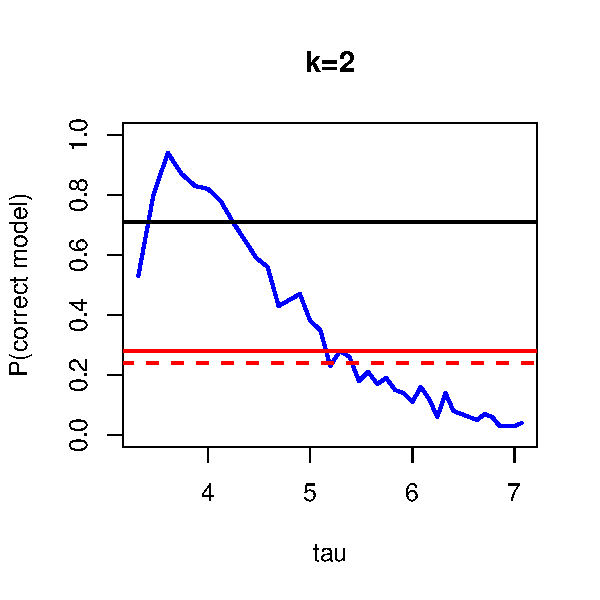
\includegraphics[width=0.32\textwidth]{Chapter-evalue/simplotmoon2}
	& 
		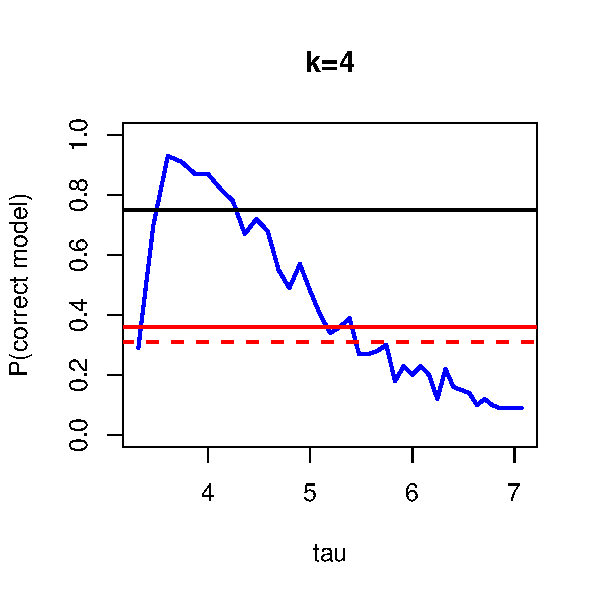
\includegraphics[width=0.32\textwidth]{Chapter-evalue/simplotmoon4} \\
	(a) & (b) \\	
		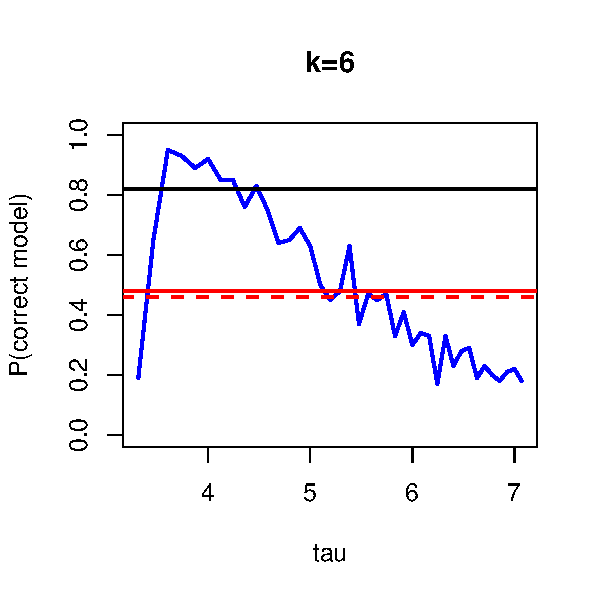
\includegraphics[width=0.32\textwidth]{Chapter-evalue/simplotmoon6}
	& 
		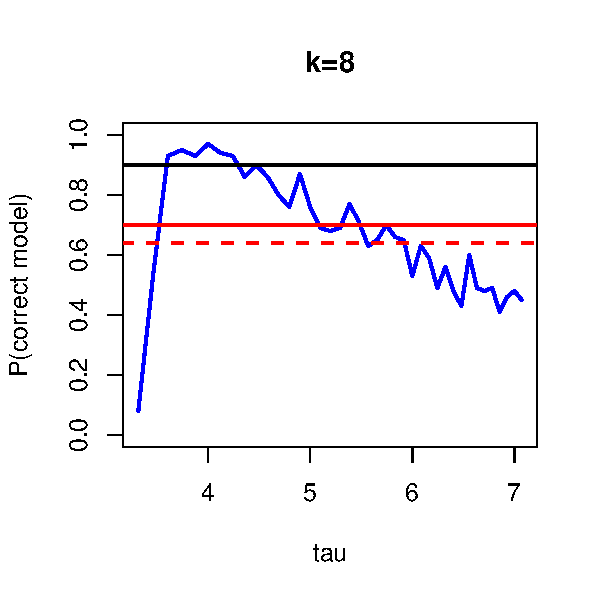
\includegraphics[width=0.32\textwidth]{Chapter-evalue/simplotmoon8} \\
	(c) & (d) \\	
\end{tabular}

\caption{Empirical probabilities of selecting the correct model through moon bootstrap for several levels of sparsity:  The $e$-values method- blue solid, AIC backward deletion- red dotted, AIC all subset- red solid, BIC backward deletion- black dotted, BIC all subset- black solid}
\label{fig:simplotsmoon}

\end{center}
\end{figure}

\begin{figure}
\begin{center}

\begin{tabular}{cc}
		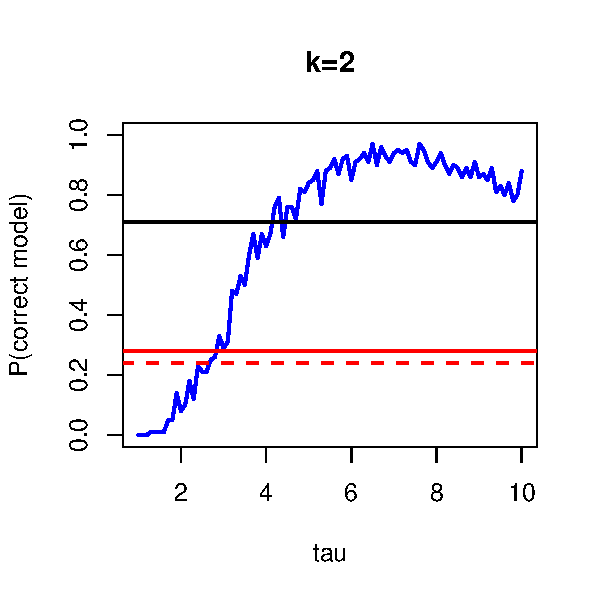
\includegraphics[width=0.32\textwidth]{Chapter-evalue/simplot_gamma2}
	& 
		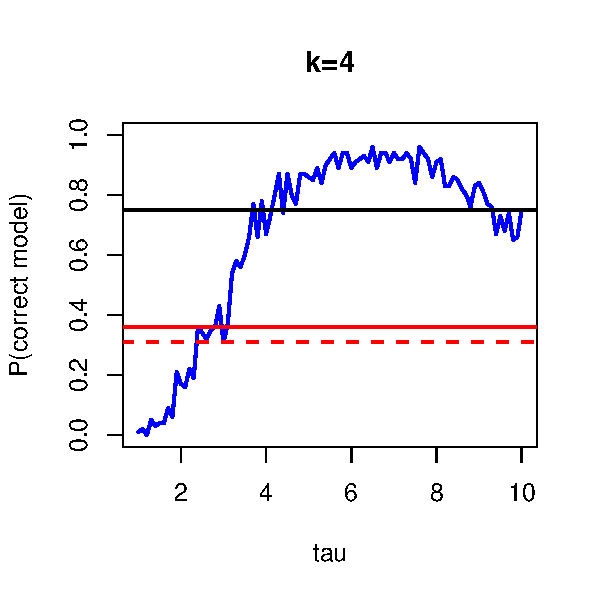
\includegraphics[width=0.32\textwidth]{Chapter-evalue/simplot_gamma4} \\
	(a) & (b) \\	
		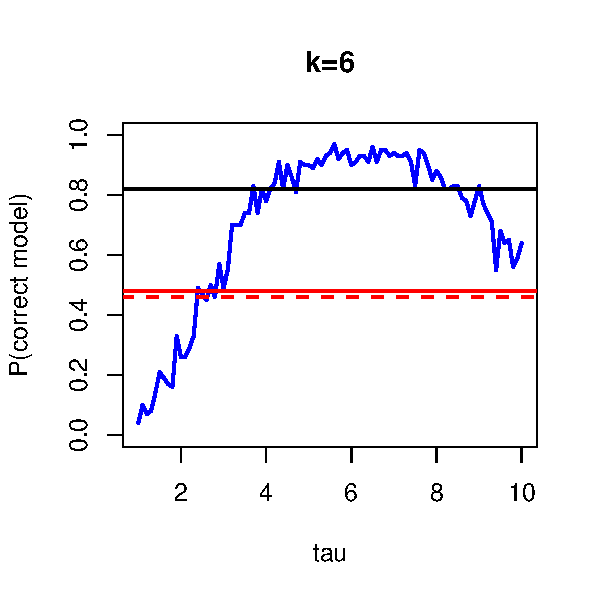
\includegraphics[width=0.32\textwidth]{Chapter-evalue/simplot_gamma6}
	& 
		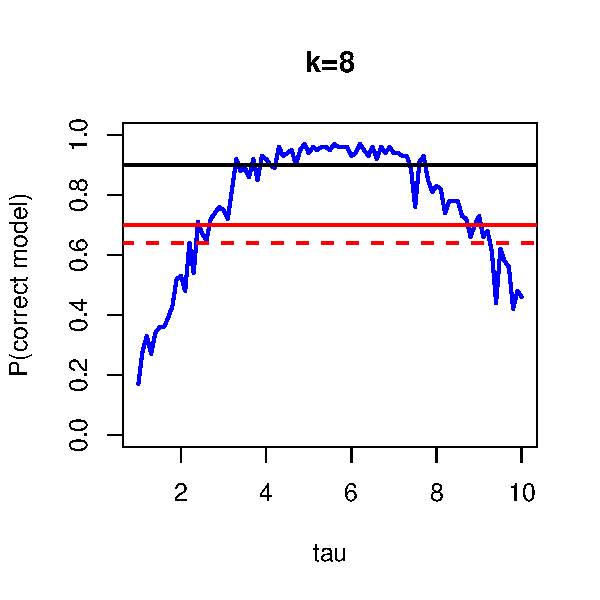
\includegraphics[width=0.32\textwidth]{Chapter-evalue/simplot_gamma8} \\
	(c) & (d) \\	
\end{tabular}

\caption{Empirical probabilities of selecting the correct model through gamma bootstrap for several levels of sparsity:  The $e$-values method- blue solid, AIC backward deletion- red dotted, AIC all subset- red solid, BIC backward deletion- black dotted, BIC all subset- black solid}
\label{fig:simplotsgamma}

\end{center}
\end{figure}

\begin{figure}
\begin{center}

\begin{tabular}{cc}
		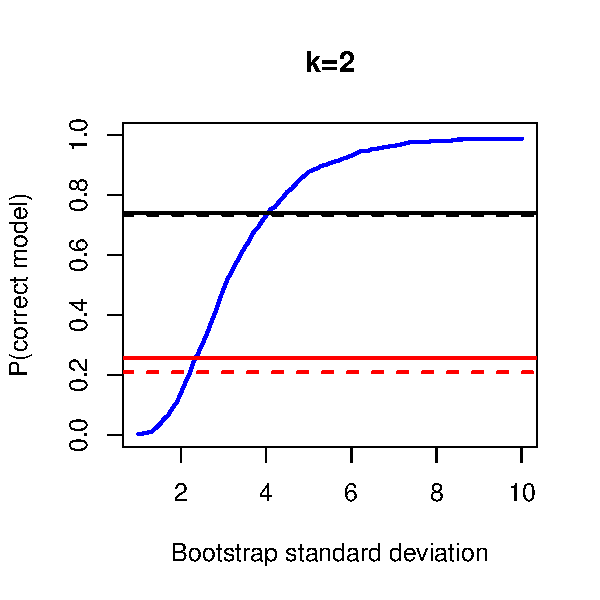
\includegraphics[width=0.32\textwidth]{Chapter-evalue/simplot2}
	& 
		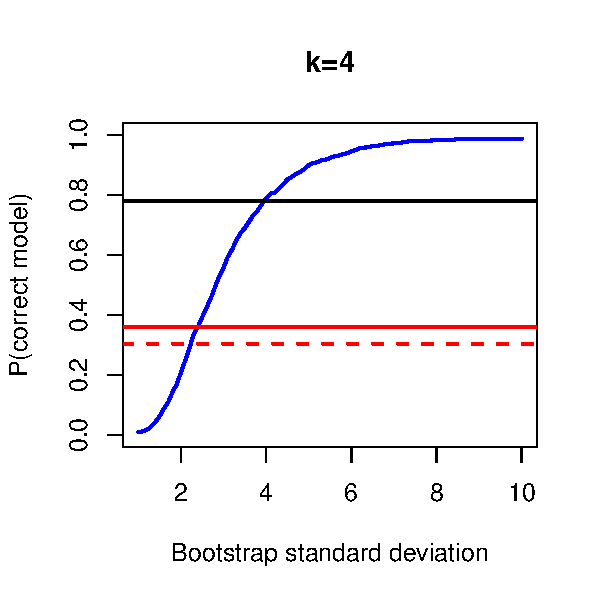
\includegraphics[width=0.32\textwidth]{Chapter-evalue/simplot4} \\
	(a) & (b) \\	
		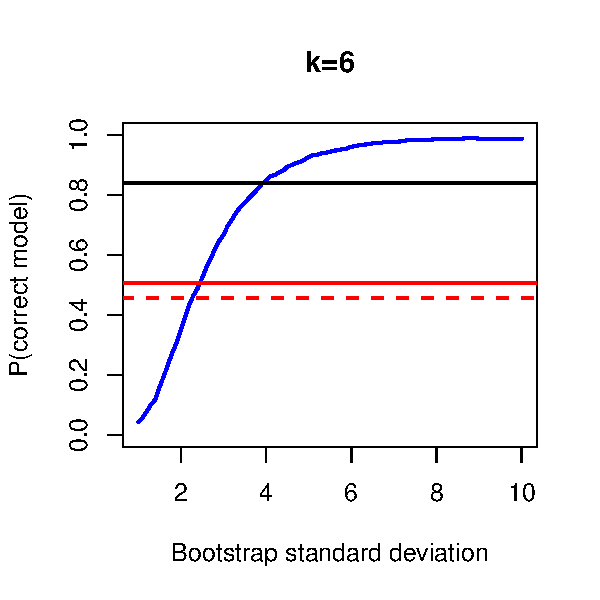
\includegraphics[width=0.32\textwidth]{Chapter-evalue/simplot6}
	& 
		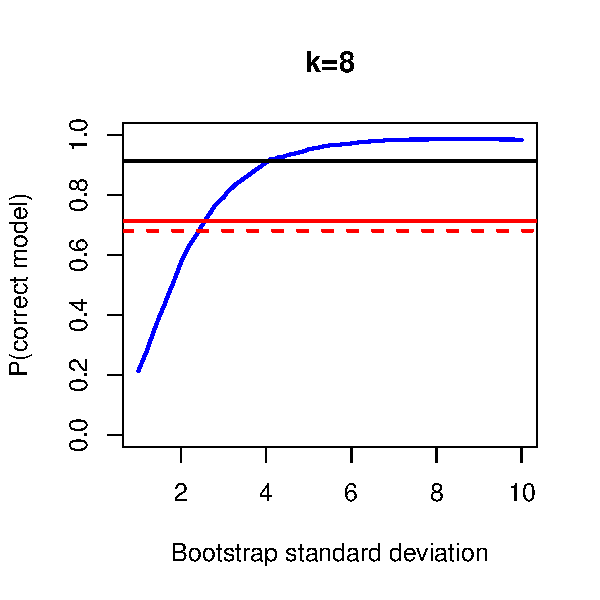
\includegraphics[width=0.32\textwidth]{Chapter-evalue/simplot8} \\
	(c) & (d) \\	
\end{tabular}

\caption{Empirical probabilities of selecting the correct model through wild bootstrap for several levels of sparsity:  The $e$-values method- blue solid, AIC backward deletion- red dotted, AIC all subset- red solid, BIC backward deletion- black dotted, BIC all subset- black solid}
\label{fig:simplotswild}

\end{center}
\end{figure}

We use the backward deletion and all-subset regression search strategies while using AIC and BIC as the model selection criterion. We use the leaps-and-bound algorithm, implemented in the {\texttt{R}} package \texttt{leaps}, for all-subset search. We display the results of this study in \ref{fig:simplotsmoon} for the moon bootstrap, in \ref{fig:simplotsgamma} for the gamma bootstrap and \ref{fig:simplotswild} for a wild bootstrap \citep{Mammen93} version of the linear regression equivalent of \ref{equation:LMMBootEqn} with i.i.d. $N(0,1)$ weights. In all three methods, and for all of $k \in \{2, 4, 6, 8 \}$ the proposed $e$-value based method performs better than AIC or BIC, as long as $\tau_{n}^{2}$ is not too small or too large. This is entirely as expected. The parametric wild bootstrap procedure has the best performance among the three, giving almost perfect detection for even very large values of $\tau_n$.
%Also interestingly, unlike the AIC or BIC, the proposed {\textit{e-value}}-based 
%procedure has the same level of accuracy in detecting the correct model regardless 
%of the amount of sparsity in $\bfbeta$. 
We experimented with other choices of $n, p, R_{1}, R_{2}$, and it seems considering $\tau \in (4, 8)$ 
in this problem ensures exact minimal adequate model selection with high chance, and typically better performance than BIC in this regard. As long as $R$ and $R_{1}$ are of the order of a few hundreds or higher, the variation from the resampling Monte Carlo step seems ignorable.

\subsection{Model selection in the presence of random effects}
Here we use the repeated measures simulation setup from \cite{PengLu12}, which has 9 fixed effects and 4 random effects, with true $\bfbeta = (0,1,1,0,0,0,0,0,0)$ and random effect covariance matrix:
%
\begin{align*}
D = \left(
	\begin{tabular}{cccc}
		9 & ~ & ~ & ~\\
		4.8 & 4 & ~ & ~\\
		0.6 & 1 & 1 & ~\\
		0 & 0 & 0 & 0\\
	\end{tabular}
	\right)
\end{align*}	
%
The error variance $\sigma^2$ is set at 1. The goal is to select the covariates of the fixed effect, thus essentially identify the covariates corresponding to the entries where $\bfbeta$ is non-zero. We use two scenarios for our study: one where the number of subjects considered is $m = 30$,  and the number of observations per subject is $n_i = 5$, and another with 60 subjects and 10 observations per subject.

%The model for the $i^\text{th}$ subject can be written as:
%%
%$$ \bfy_i = X_i \bfbeta + \bfepsilon_i $$
%%
%where $\bfepsilon_i \sim \mathcal N_{n_i} ({\bf 0}, \sigma^2 I + Z_i D Z_i^T)$. We use wild bootstrap on these residuals, so that the bootstrap equivalent of the response will be $\bfy_i^b = X_i \hat\bfbeta_{n,\text{LMM}} + u_{ib} (\bfy_i - X_i \hat\bfbeta_{n,\text{LMM}})$; with $u_{ib} \sim N(0, \tau^2)$. We take the bootstrap standard deviation $\tau = 1,2,...,8$, and determine the accuracy of our method by four measures: 

We consider $\tau \in \{1, \ldots, 15 \}$ here, and use the approximation in \ref{equation:LMMBootEqn} to calculate the bootstrapped coefficients. We consider multiple characteristics of the model that obtains the highest $e$-value, including the number of parameters it involves, the proportion of times the minimal adequate model is 
obtained, the proportion of times a zero-valued (non-zero-valued) element of beta was identified as non-zero (zero), that is, the proportion of false positives (negatives), and so on.   

In the method proposed by \cite{PengLu12}, the tuning parameter can be selected using several different criteria. We present the false positive percentage (FPR\%), false negative percentage (FNR\%) and model sizes corresponding to 
four such criteria. Our results are presented in  \ref{table:simtable1}. It can be seem the $e$-value based method handsomely outperforms the  method proposed by \cite{PengLu12}, especially in smaller sample sizes, as long as $\tau \geq 4$. 

\begin{table}[t]
	\centering
	\begin{scriptsize}
   \begin{tabular}{ll|lll|lll}
    \hline
    Method      & Tuning     & FPR\% & FNR\% & Model size & FPR\% & FNR\% & Model size \\ \cline{3-8}
    ~ & ~ & \multicolumn{3}{l|}{$n_i=5,m=30$} & \multicolumn{3}{l}{$n_i=10,m=60$}\\ \hline
  $e$-value based       & $\tau=1$      & 59.9     & 0.0   & 5.61       & 44.3     & 0.0   & 4.43       \\
    ~      & $\tau=2$      & 33.0     & 0.0   & 3.45       & 15.5     & 0.0   & 2.54       \\
    ~      & $\tau=3$      & 15.9     & 0.0   & 2.59       & 5.2      & 0.0   & 2.17       \\
    ~      & $\tau=4$      & 8.0      & 0.0   & 2.28       & 2.8      & 0.0   & 2.09       \\
    ~      & $\tau=5$      & 5.2     & 0.0   & 2.18       & 2.0   & 0.0   & 2.06       \\
    ~      & $\tau=6$      & 2.7     & 0.0   & 2.09       & 0.7   & 0.0   & 2.02       \\
    ~      & $\tau=7$      & 2.2   & 0.0   & 2.07       & 0.3   & 0.0   & 2.01       \\
    ~      & $\tau=8$      & 1.5   & 0.0   & 2.05       & 0.3   & 0.0   & 2.01       \\
    ~      & $\tau=9$      & 1.0   & 0.0   & 2.03       & 0.3   & 0.0   & 2.01       \\
    ~      & $\tau=10$      & 0.7   & 0.0   & 2.02       & 0.3   & 0.0   & 2.01       \\
    ~      & $\tau=12$      & 0.7   & 0.0   & 2.02       & 0.0   & 0.0   & 2.00       \\
    ~      & $\tau=15$      & 0.7   & 0.0   & 2.02       & 0.0   & 0.0   & 2.00       \\
     \hline
    \cite{PengLu12} & BIC    & 21.5  & 9.9   & 2.26       & 1.5   & 1.9   & 2.10       \\
    ~      & AIC    & 17    & 11.0  & 2.43       & 1.5   & 3.3   & 2.20       \\
    ~      & GCV    & 20.5  & 6     & 2.30       & 1.5   & 3     & 2.18       \\
    ~      & $\sqrt{\log n/n}$ & 21    & 15.6  & 2.67       & 1.5   & 4.1   & 2.26       \\ \hline
    \end{tabular}
    \caption{Comparison between our method and that proposed by \cite{PengLu12} through average false positive percentage, false negative percentage and model size}
    \label{table:simtable1}
    \end{scriptsize}
\end{table}
%
\begin{table}[t]
	\centering
	\begin{scriptsize}
    \begin{tabular}{llll}
    \hline
    Method          & ~ & Setting 1 & Setting 2 \\ \hline
    $e$-value based     & $\tau=1$ & 3         & 14       \\
    ~               & $\tau=2$ & 30      & 60        \\
    ~               & $\tau=3$ & 61        & 86      \\
    ~               & $\tau=4$ & 79        & 92      \\
    ~               & $\tau=5$ & 87        & 94       \\
    ~               & $\tau=6$ & 93      & 98       \\
    ~               & $\tau=7$ & 94       & 99       \\
    ~               & $\tau=8$ & 96       & 99       \\
    ~               & $\tau=9$ & 97       & 99       \\
    ~               & $\tau=10$ & 98       & 99       \\
    ~               & $\tau=12$ & 98       & 100       \\
    ~               & $\tau=15$ & 98       & 100       \\\hline
    \cite{BondellKrishnaGhosh10} & ~ & 73        & 83        \\
    \cite{PengLu12}         & ~ & 49        & 86        \\
    \cite{FanLi12}           & ~ & 90        & 100       \\ \hline
    \end{tabular}
    \caption{Comparison of our method and three sparsity-based methods of mixed effect model selection through accuracy of selecting correct fixed effects}
	\label{table:simtable2MS}
    \end{scriptsize}
\end{table}

We also compare the percentages of times the correct model was identified, and these results are presented in \ref{table:simtable2MS}, along with the corresponding results from two other papers. The proposed $e$-value based procedure performs best here for $\tau \geq 6$ for the smaller sample setting, and for $\tau\geq 12$ for larger sample setting. 


\section{Discussion and conclusion}
\label{Section:Conclusion}

In the above sections we present an expansive framework and principle, where the definition of a statistical model is very broad, and estimation procedures and resampling algorithms very general. In such a scenario, we propose a scheme of simultaneous model selection and resampling-based inference, using the newly defined $e$-value. An extremely fast algorithm, based on using data depth as evaluation function, obtains consistent true model selection  through fitting a single model. Simulation results show that the procedure performs better than traditional methods in two illustrative examples. Last but not least we provide a number of theoretical results for characterization of our method in both pupulation and sample setting.

While the above framework is extremely open-ended, multiple details require cautious approach and more detailed studies. The choice of the resampling algorithm, and the method of choosing the tuning parameter $\tau_{n}$ associated with it should be subject to further scrutiny. Our results suggest excellent {\textit{asymptotic}} properties that seem to be borne out in our simulation experiments, but finite-sample performance of our procedure needs further study. We have remarked earlier that uniform convergence, local asymptotics and detailed asymptotic studies are needed to understand the workings of our proposal more thoroughly. The current framework includes {\textit{dimension asymptotics}} where the parameter dimensions are allowed to grow with the sample size, but we do not include extremely  high-dimensional parameters in our study. The sensitivity of the results to the choice  of the evaluation maps, and the way $E_{n} (\bfy, [\bfY])$ is summarized to obtain the $e$-value deserve further attention. A further, perhaps philosophical, issue to look into is the sensitivity of the results to the choice of the preferred model. While in practice this may not matter much, the choice of the preferred model reflects a choice of paradigms and scientific principles.

In recent times, there is a growing concern about statistical inference after the implementation of a model selection step. Discussions and several interesting results relating to this matter may be found in  \cite{Yang05, LeebPotscher05, ChangEtal14, TibshiraniEtal15, Tibshiranietal16} and several references therein. The general principle discussed in this chapter advocates obtaining consistent resampling-based distributions of the estimators of {\textit{all}} parameters from {\textit{all}} candidate models. Thus in our framework, statistical inference is not the usual two-step procedure where the first step involves selection of a model, and the second  step of actual inference somehow adjusts for the uncertainties of the first step. Our proposal is one of a {\textit{joint selection and inference}} procedure, where the consistent resampling-based approximations of the sampling distributions of any collection of models are simultaneously used for inference, as well as establishing an $e$-value of a model, which may be used to preferentially treat a subset of models. 

A study of the research on post model selection inference reveals that some of the issues there may be addressed using {\textit{uniform convergence}} and related ideas. Based on the concepts and tools presented in this chapter, we have the ingredients at hand to conduct such studies.
%% on uniform convergence 
% and have already obtained some results on the conditions under which the proposed 
% {\textit{e-value}}-based procedures achieve multiple targets of optimal inference. 
%% on when and how such uniform consistency results may be obtained. 
% However, 
%We postpone discussion and presentation of such results to a future chapter. This is primarily because that arm of study involves several other technical steps, which will greatly increase the length of this manuscript and defeat 
% any attempt at clarity or conciseness. 
% 
Additionally, current studies essentially conclude that the goal of identifying the true data-generating model with probability tending to one, under the assumption that it is already one of the candidate models. This is not immediately compatible with several other goals of optimal statistical inference. Note that the problem of identification of one of the candidate models as a `true model' has not been a goal of this chapter, although our theoretical and numeric results establish that such identification is achieved easily if such a situation were to arise. We also note that traditional `true statistical model' considered in some related literature typically do not consider the domain scientific knowledge or background, and are solely based on a limited version of parsimony. Keeping this in mind, we plan to investigate the application of $e$-values to achieve multiple targets of optimal inference.

%
%What will make this fail? 
%
%\begin{enumerate}
%\item Bootstrap (or other distribution approximation method) not being good enough.
%
%\item Infinite dimensional parameters. 
%
%\item No clear choice of what should eb a preferred model: ie, should we model the mean or the median type basic issues.
%\end{enumerate}

\section{Proofs}
\label{evalues-proofs}

\begin{proof}[Proof of theorem \ref{Theorem:ThmRightWrong}]
\textit{Part 1} follows directly from assumption (E3).

\textit{Part 2.}
Assuming now that $\cM_n$ is an adequate model, we again use the location invariance property of $E_n$:
%
\begin{align}
E_n ( \hat\bfG_{mn}, [ \hat\bfG_n]) = E_n \left( \hat\bfG_{mn} - \bfG_{* n}, \left[ \hat\bfG_{* n} - \bfG_{* n} \right] \right)
\end{align}
%
and decompose the first argument
%
\begin{align}\label{equation:ThmRightWrongProofPart2Eqn1}
\hat\bfG_{mn} - \bfG_{* n} = ( \hat\bfG_{mn} - \hat \bfG_{* n} ) + ( \hat \bfG_{* n} - \bfG_{* n} )
\end{align}
%

Now we have, for any $\cM_n$,
%
$$
\hat \bftheta_{m n} \equiv \hat\bftheta = \bftheta + a_{n}^{-1} \bfT_{n} \equiv \bftheta_{m n} + a_{s n}^{-1} \bfT_{m n}
$$
%
where $\bfT_{m n}$ is distributed as $\BT_{s n}$ in $\cS_n$ indices and fixed to 0 in other indices. In terms of these, we can write the $j$-th element of $\bfG_{m n}(.) \equiv \bfG(.)$ as
%
\begin{align*}
G_{j}  (\hat{\bftheta}  )
 = G_{j}  ( {\bftheta}  )
+ a_{n}^{-1} \bfG_{1 j}^{T}  ( {\bftheta}  ) \bfT_{ n} 
+ 2 a_{n}^{-2} \bfT_{ n}^{T} \bfR_{j}   ( \hat{\bftheta}, \bfT_{ n}  ) \bfT_{ n}
\end{align*}
%
Our technical conditions are sufficient to ensure that for any $\bfc \in \BR^{d_n}$ with 
$\| \bfc \| = 1$
\begin{align*} 
\BE \left( \sum_{j =1}^{d_{n}} c_{j} \bfT_{ n}^{T} \bfR_{j}   ( \hat{\bftheta}, \bfT_{ n}  ) \bfT_{ n} \right)^{2} = O (a_{n} d_{n}) 
\end{align*}
we omit the details of the algebra here.

Thus we have that $a_n ( \hat\bfG - \bfG ) = \bfG_1^T \bfT_n + \bfR_n$, with $\BE \|\bfR_n^2 \| = o(1)$. Coming back to the first summand of the right-hand side in \ref{equation:ThmRightWrongProofPart2Eqn1} we get
%
\begin{align}\label{equation:ThmRightWrongProofPart2Eqn2}
\hat \bfG_{m n} - \hat \bfG_{* n} = \bfG_{m n} - \bfG_{* n} + O_P(\min \{ a_{s n}, a_{* n} \}^{-1})
\end{align}
%
Since $\cM_n$ is an adequate model, $ \bfG_{m n} - \bfG_{0 n} = o(n)$. Also $ \bfG_{* n} - \bfG_{0 n} = o(n)$. Thus, substituting the above right-hand side in \ref{equation:ThmRightWrongProofPart2Eqn1} we get
%
\begin{align}
\left| E_n \left( \hat\bfG_{mn} - \bfG_{* n}, \left[ \hat\bfG_{* n} - \bfG_{* n} \right] \right) - E_n \left( \hat\bfG_{* n} - \bfG_{* n}, \left[ \hat\bfG_{* n} - \bfG_{* n} \right] \right) \right| \notag\\
= o_P (\min \{ a_{s n}, a_{* n}, n \})
\end{align}
%
from of Lipschitz continuity of $E_n$. Adding back $\bfG_{* n}$ everywhere and applying (E1) again,
\begin{align}
| E_n ( \hat\bfG_{mn}, [ \hat\bfG_{* n} ] ) - E_n ( \hat\bfG_{* n}, [ \hat\bfG_{* n} ] ) | = o_P (\min \{ a_{s n}, a_{* n}, n \})
\end{align}
%
the proof of part 2 is immediate now.

{\it Part 3.} 
Since the evaluation map $E_n$ is invariant under location and scale transformations, we have
%
\begin{align}\label{equation:ThmRightWrongProofEqn1}
E_n ( \hat\bfG_{mn}, [ \hat\bfG_n]) = E_n \left( a_{* n} (\hat\bfG_{mn} - \bfG_{* n}), \left[ a_{* n} (\hat\bfG_{* n} - \bfG_{* n}) \right] \right)
\end{align}
%
Decomposing the first argument,
%
\begin{align}
a_{* n} (\hat\bfG_{mn} - \bfG_{* n}) = \frac{a_{* n}}{a_{s n}} . a_{s n} (\hat\bfG_{mn} - \bfG_{mn}) + a_{* n} (\bfG_{mn} - \bfG_{0 n}) + a_{* n} (\bfG_{0 n} - \bfG_{* n}) 
\end{align}
%
Since $\cM_n$ is inadequate, given $\delta > 0$ there exists a subsequence indexed by $\{ k_n \}$ such that $\| \bfG_{mk_n} - \bfG_{0 k_n} \| > \delta $. Since $a_{* n} \uparrow \infty$, this implies $a_{* n} \| \bfG_{mn} - \bfG_{0 n} \| \raro \infty$. Finally $ a_{* n} (\hat\bfG_{m n} - \bfG_{m n}) = O_P (1)$ using similar arguments as in proof of part 2 above, $a_{s n} \asymp a_{* n}$, and norm of the third part goes to 0 by part b of assumption (S1). We now get the needed by assumption (E4).
\end{proof}

\begin{proof}[Proof of Theorem \ref{Theorem:ResamplingConsistency_Smooth}]

We consider a generic point $\bftheta = \bftheta_{ s n} + \bfA_{ s n}^{-1} \bft$. From the Taylor series expansion, we have
%
\begin{align}
\Psi_{0 s n i (a)} (\bftheta) & = \Psi_{0 s n i (a)} (\bftheta_{s n}) 
	+ \Psi_{1 s n i (a)} (\bftheta_{s n}) \bfA_{ s n}^{-1} \bft 
+ 2^{-1}  \bft^{T} \bfA_{ s n}^{-1T} \Psi_{2 s n i (a)} (\tilde{\bftheta}_{s n} ) 
\bfA_{ s n}^{-1} \bft
\end{align}
%
for $a = 1, \ldots, p_{sn}$, and $\tilde{\bftheta}_{s n} = {\bftheta}_{s n}  + c \bfA_{s n}^{-1} \bft$ for some $c \in (0, 1)$.

Recall our convention that for any function $\bfh (\bftheta)$ evaluated at the true parameter value $\bftheta_{ s n}$, we use the notation $\bfh \equiv \bfh (\bftheta_{s n})$. Also define the $p_{ s n}$ dimensional vector 
$\bfR_{ s n} (\tilde{\bftheta}_{s n },  \bft)$ whose $a$-th element is given by 
\begin{align} 
\bfR_{ s n (a)} (\tilde{\bftheta}_{s n},  \bft)
=  \bft^{T} \bfA_{ s n}^{-1T} 
\sum_{i =1}^{k_{n}} \Psi_{2 s n i (a)} (\tilde{\bftheta}_{s n} ) \bfA_{ s n}^{-1} \bft
\end{align}

Thus we have 
\begin{align}
& p_{s n}^{-1/2} \bfA_{ s n}^{-1} \sum_{i = 1}^{ k_{n}} \Psi_{0 s n i} 
(\bftheta_{ s n} + \bfA_{ s n}^{-1} \bft) \notag\\
& = p_{s n}^{-1/2} \bfA_{ s n}^{-1} \sum_{i = 1}^{ k_{n}} \Psi_{0 s n i}  
	+  p_{s n}^{-1/2} \bfA_{ s n}^{-1} \sum_{i = 1}^{ k_{n}} \Psi_{1 s n i} \bfA_{ s n}^{-1} \bft 
+ 2^{-1}  p_{s n}^{-1/2} \bfA_{ s n}^{-1} \bfR_{ s n} (\tilde{\bftheta}_{s n },  \bft) \notag\\
& = p_{s n}^{-1/2} \bfA_{ s n}^{-1} \sum_{i = 1}^{ k_{n}} \Psi_{0 s n i}  
	+ p_{s n}^{-1/2} \bfA_{ s n}^{-1} \bfGamma_{1 s n } \bfA_{ s n}^{-1} \bft 
 + p_{s n}^{-1/2} \bfA_{ s n}^{-1} 
 \bigl( \sum_{i = 1}^{ k_{n}} \Psi_{1 s n i} - \bfGamma_{1 s n } \bigr) 
 \bfA_{ s n}^{-1} \bft \notag\\
& \quad + 2^{-1} p_{s n}^{-1/2}  \bfA_{ s n}^{-1} \bfR_{ s n} (\tilde{\bftheta}_{s n },  \bft)
\end{align}

Fix $\epsilon > 0$. We first show that there exists a $C_{0} > 0$ such that
%
\begin{equation} 
\BP \Bigl[ 
\| p_{s n}^{-1/2}  \bfA_{ s n}^{-1}  \sum_{i = 1}^{ k_{n}} \Psi_{0 s n i} \| 
> C_{0} 
\Bigr] 
< \epsilon/2.
\label{eq:Bound1}
\end{equation}
For this, we compute 
\begin{align}
p_{s n}^{-1} 
\BE \| \bfA_{ s n}^{-1}  \sum_{i = 1}^{ k_{n}} \Psi_{0 s n i} \|^{2} & = p_{s n}^{-1} \BE  \sum_{i, j = 1}^{ k_{n}} \Psi_{0 s n i}^{T} \bfA_{ s n}^{-1T} \bfA_{ s n}^{-1}   \Psi_{0 s n j} \notag\\
& = p_{s n}^{-1} \Tr \left[ \bfA_{ s n}^{-1T} \bfA_{ s n}^{-1} \right]
\BE  \sum_{i = 1}^{ k_{n}} \Psi_{0 s n i} \Psi_{0 s n i}^{T} \notag\\
& = p_{s n}^{-1} \Tr \left[ \bfA_{ s n}^{-1T} \bfA_{ s n}^{-1}  \bfGamma_{0 s n} \right] \notag\\
& = O (1)
\end{align} 
from assumption \ref{eq:Trace}. 
 
Now define
% 
\begin{align} 
\bfS_{s n} (\bft) = 
p_{s n}^{-1/2} \bfA_{ s n}^{-1} \bigl( \sum_{i = 1}^{ k_{n}} \Psi_{0 s n i} 
(\bftheta_{ s n} + \bfA_{ s n}^{-1} \bft) 
- \sum_{i = 1}^{ k_{n}} \Psi_{0 s n i}  \bigr) 
- p_{s n}^{-1/2}  \bfGamma_{1 s n }^{-1} \bfGamma_{0 s n } \bft 
\end{align}
 %
We next show that for any $C > 0$, for all sufficiently large $n$, we have
%
\begin{equation}\label{eq:Bound2}
\BE \Bigl[ \sup_{ \| \bft \| \leq C} \| \bfS_{s n} (\bft) \| \Bigr]^{2} = o (1) 
\end{equation}
%
This follows from \ref{eq:FrobSq} and \ref{eq:2ndMomentBound}.
 
Note that
%
 \begin{align} 
 \bfS_{s n} (\bft) = 
p_{s n}^{-1/2}  \bfA_{ s n}^{-1} 
 \bigl( \sum_{i = 1}^{ k_{n}} \Psi_{1 s n i} - \bfGamma_{1 s n } \bigr) 
 \bfA_{ s n}^{-1} \bft
+ 2^{-1} p_{s n}^{-1/2}  \bfA_{ s n}^{-1} \bfR_{ s n} (\tilde{\bftheta}_{s n },  \bft)
\end{align}
%
Thus
% 
\begin{align} 
& \sup_{ \| \bft \| \leq C} \| \bfS_{s n} (\bft) \| 
\leq \notag \\
& p_{s n}^{-1/2} \sup_{ \| \bft \| \leq C} \| 
 \bfA_{ s n}^{-1} 
 \bigl( \sum_{i = 1}^{ k_{n}} \Psi_{1 s n i} - \bfGamma_{1 s n } \bigr) 
 \bfA_{ s n}^{-1} \bft
\| 
+ 
2^{-1} p_{s n}^{-1/2} 
\sup_{ \| \bft \| \leq C} \| 
 \bfA_{ s n}^{-1} \bfR_{ s n} (\tilde{\bftheta}_{s n },  \bft)
\|
\end{align}
We consider each of these terms separately. 

For any matrix $\bfM \in \BR^{p \times p}$, we have
%
\begin{align} 
\sup_{ | \bft| \leq C} \| \bfM \bft \| 
& = \sup_{ \| \bft \| \leq C} 
\Bigl[ \sum_{i =1}^{p} \bigl( \sum_{j =1}^{p} m_{ i j} t_{j} \bigr)^{2} \Bigr]^{1/2} \notag\\
& \leq \sup_{ \| \bft \| \leq C} 
\Bigl[ \sum_{i =1}^{p} \sum_{j =1}^{p} m_{ i j}^{2} 
\sum_{j =1}^{p} t_{j}^{2} \Bigr]^{1/2} \notag\\
& = \| \bfM \|_{F} \sup_{ \| \bft \| \leq C} \|\bft \| \notag\\
& = C \| \bfM \|_{F}
\end{align}
%
Using $\bfM =  \bfA_{ s n}^{-1}  \bigl( \sum_{i = 1}^{ k_{n}} \Psi_{1 s n i} - \bfGamma_{1 s n } \bigr) \bfA_{ s n}^{-1}$ and \ref{eq:FrobSq}, we get one part of the result.

For the other term, we similarly have 
%
\begin{align} 
\Bigl[ \sup_{ \| \bft \| \leq C} \| 
p_{s n}^{-1/2}  \bfA_{ s n}^{-1} \bfR_{ s n} (\tilde{\bftheta}_{s n },  \bft)
\| \Bigr]^{2} & = p_{s n}^{-1} \sup_{ \| \bft \| \leq C} 
\Bigl[ \|  \bfA_{ s n}^{-1} \bfR_{ s n} (\tilde{\bftheta}_{s n },  \bft)
\| \Bigr]^{2} \notag\\
& \leq p_{s n}^{-1} \lambda_{max}\bigl( \bfA_{ s n}^{-1T} \bfA_{ s n}^{-1}  \bigr)
\sup_{ \| \bft \| \leq C} \| \bfR_{ s n} (\tilde{\bftheta}_{s n },  \bft)\|^{2} \notag\\
& \leq p_{s n}^{-1} \lambda_{max}\bigl( \bfA_{ s n}^{-1} \bfA_{ s n}^{-1T}  \bigr)
\sup_{ \| \bft \| \leq C} \| \bfR_{ s n} (\tilde{\bftheta}_{s n },  \bft)\|^{2} \notag\\
& \leq p_{s n}^{-1} a_{s n}^{-2} 
\sup_{ \| \bft \| \leq C} \| \bfR_{ s n} (\tilde{\bftheta}_{s n },  \bft)\|^{2}
\end{align}

%Now for $\| \bfA_{ s n}^{-1}  \|_{F}$ we have 
%\begin{align} 
%\| \bfA_{ s n}^{-1}  \|_{F} & = 
%\Tr \bigl( \bfA_{ s n}^{-1T} \bfA_{ s n}^{-1} \bigr) \\
%& =  \Tr \bigl( \bfGamma_{1 s n }^{-1} \bfGamma_{0 s n } \bfGamma_{1 s n }^{-1T} \bigr) \\
%& \leq    O \Bigl( p_{s n} 
%\lambda_{max} \bigl( \bfGamma_{1 s n }^{-1} \bfGamma_{0 s n } \bfGamma_{1 s n }^{-1T} \bigr) 
%\Bigr) \\
%& \leq    O \bigl( p_{s n} a_{s n}^{-2} \bigr). 
%\end{align}

Note that 
\begin{align} 
\bigl( \sup_{ \| \bft \| \leq C} \| \bfR_{ s n} (\tilde{\bftheta}_{s n },  \bft)\| \bigr)^{2}
= 
\sup_{ \| \bft \| \leq C} \| \bfR_{ s n} (\tilde{\bftheta}_{s n },  \bft)\|^{2}
\end{align}
%
Now
%
\begin{align} 
\| \bfR_{ s n} (\tilde{\bftheta}_{s n },  \bft)\|^{2} & = 
\sum_{a = 1}^{ p_{s n}} 
\bigl( \bfR_{ s n (a)} (\tilde{\bftheta}_{s n},  \bft) \bigr)^{2} \notag\\
& = 
\sum_{a = 1}^{ p_{s n}} 
\bigl( 
\bft^{T} \bfA_{ s n}^{-1T} 
\sum_{i =1}^{k_{n}} \Psi_{2 s n i (a)} (\tilde{\bftheta}_{s n} ) \bfA_{ s n}^{-1} \bft
\bigr)^{2} \notag\\
& = 
\sum_{a = 1}^{ p_{s n}} 
\sum_{i, j = 1}^{ k_{n}} 
\bft^{T} \bfA_{ s n}^{-1T} \Psi_{2 s n i (a)} (\tilde{\bftheta}_{s n} ) \bfA_{ s n}^{-1} \bft.
\bft^{T} \bfA_{ s n}^{-1T} \Psi_{2 s n j (a)} (\tilde{\bftheta}_{s n} ) \bfA_{ s n}^{-1} \bft
\end{align} 
%
Based on this, we have
%
\begin{align} 
\sup_{ \| \bft \| \leq C} \| \bfR_{ s n} (\tilde{\bftheta}_{s n },  \bft)\|^{2} & = \sup_{ \| \bft \| \leq C} 
\sum_{a = 1}^{ p_{s n}} 
\sum_{i, j = 1}^{ k_{n}} 
\bft^{T} \bfA_{ s n}^{-1T} \Psi_{2 s n i (a)} (\tilde{\bftheta}_{s n} ) \bfA_{ s n}^{-1} \bft.
\bft^{T} \bfA_{ s n}^{-1T} \Psi_{2 s n j (a)} (\tilde{\bftheta}_{s n} ) \bfA_{ s n}^{-1} \bft
\notag\\
& \leq \sup_{ \| \bft \| \leq C} 
\sum_{a = 1}^{ p_{s n}} 
\sum_{i, j = 1}^{ k_{n}} 
\bft^{T} \bfA_{ s n}^{-1T} \bfM_{2 s n i (a)}  \bfA_{ s n}^{-1} \bft.
\bft^{T} \bfA_{ s n}^{-1T} \bfM_{2 s n j (a)}  \bfA_{ s n}^{-1} \bft
\notag\\
& \leq \sup_{ \| \bft \| \leq C} \| \bfA_{ s n}^{-1} \bft \|^{4}
\sum_{a = 1}^{ p_{s n}} 
\Bigl(
\sum_{i = 1}^{ k_{n}} 
 \lambda_{max} \bigl( \bfM_{2 s n i (a)} \bigr) \Bigr)^{2}
\notag \\
& \leq  C^{4} n \lambda_{max}^{2} \bigl( \bfA_{ s n}^{-1T} \bfA_{ s n}^{-1} \bigr)
\sum_{a = 1}^{ p_{s n}} 
\sum_{i = 1}^{ k_{n}} 
 \lambda_{max}^{2} \bigl( \bfM_{2 s n i (a)} \bigr)
 \end{align} 

Putting all these together, we have 
%
\begin{align} 
\BE \Bigl[ \sup_{ \| \bft \| \leq C} \|
 p_{s n}^{-1/2}  \bfA_{ s n}^{-1} \bfR_{ s n} (\tilde{\bftheta}_{s n },  \bft) \|
 \Bigr]^{2} & = p_{s n}^{-1}  \BE \Bigl[ \sup_{ \| \bft \| \leq C} 
  \bfA_{ s n}^{-1} \bfR_{ s n} (\tilde{\bftheta}_{s n },  \bft)
 \Bigr]^{2} \notag\\
& \leq p_{s n}^{-1}  \bfA_{ s n}^{-2}   \BE \Bigl[ \sup_{ \| \bft \| \leq C} 
  \| \bfR_{ s n} (\tilde{\bftheta}_{s n },  \bft)\|
 \Bigr]^{2} \notag\\
 & = O \bigl( p_{s n}^{-1} a_{s n}^{-2} \bigr)
 \BE \Bigl[ \sup_{ \| \bft \| \leq C} 
  \| \bfR_{ s n} (\tilde{\bftheta}_{s n },  \bft)\|
 \Bigr]^{2} \notag\\
  & = O \bigl( p_{s n}^{-1} n a_{s n}^{-6} \bigr)
\sum_{a = 1}^{ p_{s n}} 
\sum_{i = 1}^{ k_{n}} 
 \BE \lambda_{max}^{2} \bigl( \bfM_{2 s n i (a)} \bigr) \notag\\
%  & = O \bigl( p_{s n}^{2} n a_{s n}^{-6} \bigr)
%\sum_{a = 1}^{ p_{s n}} 
%\sum_{i = 1}^{ k_{n}} 
% \BE \lambda_{max}^{2} \bigl( \bfM_{2 s n i (a)} \bigr)\\
& = o(1)
\end{align}
using \ref{eq:2ndMomentBound}. 

Now define
% 
\begin{align} 
\bfS_{s n} (\bft) = 
p_{s n}^{-1/2} \bfA_{ s n}^{-1} \bigl( \sum_{i = 1}^{ k_{n}} \Psi_{0 s n i} 
(\bftheta_{ s n} + \bfA_{ s n}^{-1} \bft) 
- \sum_{i = 1}^{ k_{n}} \Psi_{0 s n i}  \bigr) 
- p_{s n}^{-1/2}  \bfGamma_{1 s n }^{-1} \bfGamma_{0 s n } \bft 
\end{align}
%
hence
% 
\begin{align} 
p_{s n}^{-1/2} \bfA_{ s n}^{-1}  \sum_{i = 1}^{ k_{n}} \Psi_{0 s n i} 
(\bftheta_{ s n} +  p_{s n}^{1/2} \bfA_{ s n}^{-1} \bft) 
= \bfS_{s n}( \bft ) + 
p_{s n}^{-1/2} \bfA_{ s n}^{-1}   \sum_{i = 1}^{ k_{n}} \Psi_{0 s n i} 
+ \bfA_{ s n}^{-1} \bfGamma_{1 s n } \bfA_{ s n}^{-1} \bft
\end{align}
%
and thus
%
\begin{align} 
& \inf_{ \| \bft \| = C} 
\Bigl\{ p_{s n}^{-1/2} 
\bft^{T} \bfGamma_{1 s n } \bfA_{ s n}^{-1}  \sum_{i = 1}^{ k_{n}} \Psi_{0 s n i} 
(\bftheta_{ s n} +  p_{s n}^{1/2} \bfA_{ s n}^{-1} \bft) 
\Bigr\} \notag\\
& = 
 \inf_{ \| \bft \| = C} 
\Bigl\{ 
\bft^{T}  \bfGamma_{1 s n } \bfS_{s n}( \bft ) + 
p_{s n}^{-1/2} \bft^{T}  \bfGamma_{1 s n }  \bfA_{ s n}^{-1}  \sum_{i = 1}^{ k_{n}} \Psi_{0 s n i}  
+ \bft^{T}  \bfGamma_{1 s n } \bfA_{ s n}^{-1} \bfGamma_{1 s n } \bfA_{ s n}^{-1} \bft
\Bigr\} \notag\\
& \geq 
 \inf_{ \| \bft \| = C} \bft^{T}  \bfGamma_{1 s n } \bfS_{s n}( \bft ) 
 + p_{s n}^{-1/2}  \inf_{ \| \bft \| = C} \bft^{T}  \bfGamma_{1 s n }  \bfA_{ s n}^{-1}  
 \sum_{i = 1}^{ k_{n}} \Psi_{0 s n i}  
 + \inf_{ \| \bft \| = C} \bft^{T}  \bfGamma_{1 s n } \bfA_{ s n}^{-1} \bfGamma_{1 s n } \bfA_{ s n}^{-1} \bft
  \notag\\
 & \geq  - C  \delta_{1 s}  \sup_{ \| \bft \| = C} \| \bfS_{s n}( \bft ) \|
- C \delta_{1 s}  p_{s n}^{-1/2}   \| \bfA_{ s n}^{-1}  \sum_{i = 1}^{ k_{n}} \Psi_{0 s n i} \| 
+ C^{2}  \delta_{0 s}
\end{align}
The last step above utilizes facts like $\bfa^{T} \bfb \geq - \|a\| \|b\|$.  

Consequently, defining $C_{1} = C \delta_{ 0 s}/\delta_{1 s}$, we have 
\begin{align} 
& \BP \Bigl[  
\inf_{ \| \bft \| = C} 
\Bigl\{ 
\bft^{T} \bfGamma_{1 s n }  \bfA_{ s n}^{-1}  \sum_{i = 1}^{ k_{n}} \Psi_{0 s n i} 
(\bftheta_{ s n} +  p_{s n}^{1/2} \bfA_{ s n}^{-1} \bft) 
\Bigr\} < 0 
\Bigr] \notag\\
\leq 
& \BP \Bigl[  
\sup_{ \| \bft \| = C} \| \bfS_{s n}( \bft ) \| + \| \bfA_{ s n}^{-1}  \sum_{i = 1}^{ k_{n}} \Psi_{0 s n i} \| 
> C_{1} 
\Bigr] \notag\\
\leq 
& \BP \Bigl[  
\sup_{ \| \bft \| = C} \| \bfS_{s n}( \bft ) \|  > C_{1}/2 \Bigr] 
+ \BP \Bigl[ 
\| \bfA_{ s n}^{-1}  \sum_{i = 1}^{ k_{n}} \Psi_{0 s n i} \| 
> C_{1}/2 
\Bigr] \notag\\
& < \epsilon 
\end{align}
for all sufficiently large $n$,  using \ref{eq:Bound1} and \ref{eq:Bound2}. 
 
This implies that with a probability greater than $1 - \epsilon$ there is a root $\bfT_{ s n}$ of the equations $\sum_{i = 1}^{ k_{n}} \Psi_{0 s n i} (\bftheta_{ s n} +  \bfA_{ s n}^{-1} \bft)$  in the ball $\{ \| \bft \| < C \}$, for some $C > 0$ and all sufficiently large $n$. Defining $\hat{\bftheta}_{ s n}  = \bftheta_{ s n} +   \bfA_{ s n}^{-1} \bfT_{s n}$, we obtain the desired result. Issues like dependence on $\epsilon$ and other technical details are handled using standard arguments, see \cite{ChatterjeeBose05} for related arguments.

Since we have
%
 \begin{align} 
 \sup_{\| \bft \| < C} \| \bfS_{s n} (\bft) \| = o_{P} (1) 
 \end{align} 
%
and $\bfT_{s n}$ lies in the set $\| \bft \| < C$, define $- \bfR_{s n} = \bfS_{s n} ( \bfT_{s n}) = o_{P} (1)$. We consequently have 
 \begin{align} 
- \bfR_{s n} & =  \bfS_{s n} ( \bfT_{s n})  \notag\\
& 
 p_{s n}^{-1/2} \bfA_{ s n}^{-1} \bigl( \sum_{i = 1}^{ k_{n}} \Psi_{0 s n i} 
(\bftheta_{ s n} + \bfA_{ s n}^{-1} \bfT_{s n}) 
- \sum_{i = 1}^{ k_{n}} \Psi_{0 s n i}  \bigr) 
- p_{s n}^{-1/2}  \bfGamma_{1 s n }^{-1} \bfGamma_{0 s n }\bfT_{s n} \notag\\
& 
 p_{s n}^{-1/2} \bfA_{ s n}^{-1} \sum_{i = 1}^{ k_{n}} \Psi_{0 s n i} 
- p_{s n}^{-1/2}  \bfGamma_{1 s n }^{-1} \bfT_{s n} 
\end{align}
Thus, 
\begin{align} 
\bfT_{s n} & = 
-  \bfGamma_{0 s n }^{-1} \bfGamma_{1 s n } 
\bfA_{ s n}^{-1}  \sum_{i = 1}^{ k_{n}} \Psi_{0 s n i} 
+ p^{1/2} \bfGamma_{0 s n }^{-1} \bfGamma_{1 s n } \bfR_{s n} \notag\\
& = 
-  \bfGamma_{0 s n }^{-1/2}  \sum_{i = 1}^{ k_{n}} \Psi_{0 s n i} 
+ p^{1/2} \bfGamma_{0 s n }^{-1} \bfGamma_{1 s n } \bfR_{s n}
\end{align}

Note that our conditions imply that for any $\bfc$ with $\| \bfc \| =1$, we have that 
 $\bfc^T \bfT_{s n}$ has two terms, where 
 $\BV \bigl( - \bfc^T \bfGamma_{0 s n }^{-1/2}  \sum_{i = 1}^{ k_{n}} \Psi_{0 s n i} 
 \bigr) = 1$ and 
 \begin{align} 
 \BE 
 \bigl[ p^{1/2} \bfc^T \bfGamma_{0 s n }^{-1} \bfGamma_{1 s n } \bfR_{s n} 
 \bigr]^{2} = O(1)
\end{align} 
using \ref{eq:Trace}. Using \ref{eq:CLTConditions} we also have that for any $\bfc$ with $\| \bfc\| = 1$, $\bfc^T \bfT_{s n} \leadsto N (0, 1)$. 

Define 
\begin{align} 
\hat{\bfA}_{s n} = \mu_{s n} \tau_{s n}^{-1} \hat{\bfGamma}_{0 s n}^{1/2}
\hat{\bfGamma}_{1 s n}^{-1}.
\end{align}

We now follow steps that are very similar to the above, but for the resampling procedure as implemented in \ref{eq:ResamplingMinimization} to obtain the result. We omit the details. 
 
\end{proof}

\begin{proof}[Proof of theorem \ref{Theorem:ModelScore}]
\textit{Part 1.}
Taking a similar approach as in the proof of theorem \ref{Theorem:ThmRightWrong}, we get
%
\begin{align*}
G_{j}  (\hat{\bftheta_r}  )
& = G_{j}  ( \hat{\bftheta}  )
+ b_{n}^{-1} \bfG_{1 j}^{T}  ( \hat{\bftheta}  ) \bfT_{r n} 
+ 2 b_{n}^{-2} \bfT_{ n}^{T} \bfR_{j}   ( \hat{\bftheta}, \bfT_{r n}  ) \bfT_{r n}, \\
& = G_{j}  ( \hat{\bftheta}  )
+ b_{n}^{-1} \bfG_{1 j}^{T}  ( {\bftheta}  ) \bfT_{r n} 
+ b_{n}^{-1}  ( \hat{\bfG}_{1 j} - \bfG_{1 j}   )^{T} \bfT_{r n} 
+ 2 b_{n}^{-2} \bfT_{r n}^{T} \bfR_{j}   ( \hat{\bftheta}, \bfT_{r n}  ) \bfT_{n}, \\
& = G_{j}  ( \hat{\bftheta}  )
+ b_{n}^{-1} \bfG_{1 j}^{T}  ( {\bftheta}  ) \bfT_{r n} 
+ b_{n}^{-1} \bfR_{r n j 1} + b_{n}^{-2} \bfR_{r n j 2}
\end{align*}
%
Our technical conditions are sufficient to ensure that for any $\bfc \in \BR^{d_n}$ with 
$\| \bfc \| = 1$
\begin{align*} 
\BE_r \left( \sum_{j =1}^{d_{n}} c_{j} \bfR_{r n j 1} \right)^{2} 
= o_P (b_{n}^{-1} d _{n}); \quad \BE_r \left( \sum_{j =1}^{d_{n}} c_{j} \bfR_{r n j 2} \right)^{2} = O_P (b_{n} d_{n}), 
\end{align*}
we omit the details of the algebra here. Thus we get $b_{ n} (\hat \bfG_r - \hat \bfG ) = \bfG_1^T \bfT_{r n} + \bfR_{r n} $ with $\BE_r \| \bfR_{r n} \|^2 = o_P(1)$. Hence
%
\begin{align}\label{eqn:ModelScoreProofEqn1}
\hat \bfG_{r m n} - \hat \bfG_{r * n} = \hat \bfG_{m n} - \hat \bfG_{* n} + O_{P_n} ( \min \{ b_{s n}, b_{* n} \}^{-1}) + o_P(1)
\end{align}
%
where $s_n = o_{P_n} (t_n)$ means $s_n / t_n \rightarrow 0$ in probability conditional on the data.

Now following assumption (E1),
%
\begin{align}\label{eqn:ModelScoreProofEqn2}
E_n ( \hat \bfG_{r m n}, [ \hat \bfG_{r_1 * n} ] ) = E_n ( ( \hat \bfG_{r m n} - \hat \bfG_{* n} ), [   \hat \bfG_{r_1 * n} - \hat \bfG_{* n} ] )
\end{align}
%
Expanding first argument of the right-hand side
%
\begin{align*}
\hat \bfG_{r m n} - \hat \bfG_{* n}  & =  ( \hat \bfG_{r m n} - \hat \bfG_{r * n} ) + ( \hat \bfG_{r * n} - \hat \bfG_{* n} )
\end{align*}
% \notag\\
%& = ( \hat \bfG_{r m n} - \hat \bfG_{m n}) - (\hat \bfG_{r_1 * n} - \hat \bfG_{* n} ) \notag\\
%& \quad + ( \hat \bfG_{m n} - \hat \bfG_{* n}) + ( \hat \bfG_{r_1 * n} - \hat \bfG_{* n} ) \notag\\
%& = ( \hat \bfG_{r_1 * n} - \hat \bfG_{* n} ) + O_{P_n} ( \min \{ b_{s n}, b_{* n} \} ) + o_{P} ( \min \{ a_{s n}, a_{* n} \} )
%
We now apply \ref{eqn:ModelScoreProofEqn1} and then \ref{equation:ThmRightWrongProofPart2Eqn2} to the first summand on the right side. Scalar invariance and lipschitz continuity of the evaluation map $E_n$ implies
%
\begin{align*}
& \left| E_n ( \hat \bfG_{r m n}, [ \hat \bfG_{r_1 * n} ] ) - E_n ( \hat \bfG_{r * n}, [ \hat \bfG_{r_1 * n} ] ) \right| \\
&= O_{P_n} ( \min \{ b_{s n}, b_{* n} \}^{-1}) + O_{P} ( \min \{ a_{s n}, a_{* n} \}^{-1})
\end{align*}
%
Finally from theorem \ref{Theorem:ResamplingConsistency_Smooth} and assumption (G2), $b_{s n} ( \hat \bfG_{r * n} - \hat \bfG_{* n} )$ and $a_{s n} ( \hat \bfG_{* n} - \bfG_{* n} )$ converge to the same limiting distribution for almost every data sequence; thus
%
\begin{align*}
\BE_r E_n ( \hat \bfG_{r * n}, [ \hat \bfG_{r_1 * n} ]) = \BE E_n ( \hat \bfG_{* n}, [ \hat \bfG_{* n} ]) + o_{P_n}(1)
\end{align*}
%
The proof follows since $\tau_{s n} = o( a_{s n}) \Rightarrow b_{s n} \raro \infty$.

\textit{Part 2.}
Continuing from \ref{eqn:ModelScoreProofEqn2} and applying scale invariance,
%
\begin{align*}
E_n ( \hat \bfG_{r m n}, [ \hat \bfG_{r_1 * n} ] ) = E_n ( b_{* n} ( \hat \bfG_{r m n} - \hat \bfG_{* n} ), [   b_{* n}  ( \hat \bfG_{r_1 * n} - \hat \bfG_{* n} ) ] )
\end{align*}
%
and then
%
\begin{align*}
b_{* n} ( \hat \bfG_{r m n} - \hat \bfG_{* n} ) & = \frac{ b_{* n} }{ b_{s n}} . b_{s n} ( \hat \bfG_{r m n} - \hat \bfG_{m n} ) + \frac{b_{* n}}{a_{s n}}. a_{s n} ( \hat \bfG_{m n} - \bfG_{m n} )  \notag\\
& \quad - \frac{b_{* n}}{a_{* n}}. a_{* n} ( \hat \bfG_{* n} - \bfG_{* n} ) + b_{* n} ( \bfG_{m n} - \bfG_{* n} )
\end{align*}

Since $b_{* n} = a_{* n} / \tau_{* n}, \tau_{* n} = o(a_{* n}), a_{* n} \asymp a_{s n}$, lipschitz continuity of $E_n$ ensures that
%
\begin{align*}
& \BE_r E_n ( b_{* n} ( \hat \bfG_{r m n} - \hat \bfG_{* n} ), [   b_{* n}  ( \hat \bfG_{r_1 * n} - \hat \bfG_{* n} ) ] ) \notag\\
& = \BE_r E_n \left( \frac{ b_{* n} }{ b_{s n}} . b_{s n} ( \hat \bfG_{r m n} - \hat \bfG_{m n} ) + b_{* n} ( \bfG_{m n} - \bfG_{* n} ), [   b_{* n}  ( \hat \bfG_{r_1 * n} - \hat \bfG_{* n} ) ] \right) \notag\\
& \qquad + o_P(1)
\end{align*}
%
From theorem \ref{Theorem:ResamplingConsistency_Smooth} and assumption (G2) $b_{s n} ( \hat \bfG_{r m n} - \hat \bfG_{m n} )$ and $a_{s n} ( \hat \bfG_{m n} - \bfG_{m n} )$ converge to the same limiting distribution for almost every data sequence; and $b_{* n} \uparrow \infty$ implies $\| b_{* n} ( \bfG_{m n} - \bfG_{* n}) \| \raro \infty$. Also by assumption $b_{* n} \asymp b_{s n}$. The proof now follows from assumption (E4).
\end{proof}

\begin{proof}[Proof of theorem \ref{Theorem:ThmRightNested}]

Since we are dealing with a finite sequence of nested models, it is enough to prove that $e_n(\cM_1 ) > e_n(\cM_2 )$ for large enough $n$.

Suppose $\BT_0 = \cE ({\bf 0}_p, \bfI_p, g)$. Affine invariance implies invariant to rotational transformations, and since depth decreases along any ray from the origin, $D( \bftheta, \BT_0)$ is a monotonocally decreasing function of $\bftheta^T \bftheta$ for any $\bftheta \in \BR^p$. Now consider the models $\cM_{10}, \cM_{20}$ that have 0 in all indices outside $\cS_1$ and $\cS_2$, respectively. Take some $\bftheta_{10} \in \bfTheta_{10}$, which is the parameter space corresponding to $\cM_{10}$, and replace its (zero) entries at indices $j \in \cS_2 \setminus \cS_1$ by some non-zero $\bfdelta \in \BR^{p - | \cS_2 \setminus \cS_1 |}$. Denote it by $\bftheta_{1 \bfdelta}$. Then we shall have
%
\begin{align*}
\bftheta_{1 \bfdelta}^T \bftheta_{1 \bfdelta} > \bftheta_{10}^T \bftheta_{10}
& \quad \Rightarrow \quad
D( \bftheta_{10}, \BT_0) > D( \bftheta_{1 \bfdelta}, \BT_0)\\
& \quad \Rightarrow \quad
\BE_{s1} D( \bftheta_{10}, \BT_0) > \BE_{s1} D( \bftheta_{1 \bfdelta}, \BT_0)
\end{align*}
%
where $\BE_s$ denotes the expectation taken over the marginal of the distributional argument $\BT_0$ at indices $\cS_1$. Notice now that by consitruction $\bftheta_{1 \bfdelta} \in \bfTheta_{20}$, the parameter space corresponding to $\cM_{20}$, and since the above holds for all possible $\bfdelta$, we can take expectation over indices $\cS_2 \setminus \cS_1$ in both sides to obtain $\BE_{s1} D( \bftheta_{10}, \BT_0) > \BE_{s2} D( \bftheta_{20}, \BT_0)$, with $\bftheta_{20}$ denoting a general element in $\bfTheta_{20}$.

Now combining (S1a) and (S1b) we get $a_n \bfV_n^{-1/2} (\hat \bftheta - \bftheta_0 ) \leadsto \BT_0$. Suppose $\BT_n := [ a_n \bfV_n^{-1/2} (\hat \bftheta - \bftheta_0 ) ]$. Now choose a positive $\epsilon < (\BE_{s1} D( \bftheta_{10}, \BT_0) - \BE_{s2} D( \bftheta_{20}, \BT_0))/2$. Then, for large enough $n$ we shall have
%
$$
\left| D( \bftheta_{10}, \BT_n) - D( \bftheta_{10}, \BT_0) \right| < \epsilon
\quad \Rightarrow \quad
| \BE_{s1} D( \bftheta_{10}, \BT_n) - \BE_{s1} D( \bftheta_{10}, \BT_0) | < \epsilon
$$
%
following condition (D4). Similarly we have $| \BE_{s2} D( \bftheta_{20}, \BT_n) - \BE_{s2} D( \bftheta_{20}, \BT_0) | < \epsilon $ for the same $n$ for which the above holds. This implies $\BE_{s1} D( \bftheta_{10}, \BT_n) > \BE_{s2} D( \bftheta_{20}, \BT_n)$.

Now apply the affine transformation $\bft (\bftheta) = \bfV_n^{1/2} \bftheta / a_n + \bftheta_0$ to both arguments of the depth function above. This will keep the depths constant following affine invariance, i.e. $D(\bft ( \bftheta_{10}), [\hat \bftheta]) = D( \bftheta_{10}, \BT_n)$ and $D(\bft ( \bftheta_{20}), [\hat \bftheta]) = D( \bftheta_{20}, \BT_n)$. Since this transformation maps $\bfTheta_{10}$ to $\bfTheta_1$, the parameter space corresonding to $\cM_1$, we get $\BE_{s1} D(\bft ( \bftheta_{10}), [\hat \bftheta]) > \BE_{s2} D(\bft ( \bftheta_{20}), [\hat \bftheta])$, i.e. $e_n ( \cM_1 ) > e_n ( \cM_2 )$.

\end{proof}

\begin{proof}[Proof of corollary \ref{Corollary:ZeroModelCorollary}]
By construction, $\cM_0$ is the unique minimal adequate model in $\mathbb M_{0}$, and should be nested in all other adequate models therein. Hence theorem \ref{Theorem:ThmRightNested} implies $e_n ( \cM_0) > e_n (\cM^c)$ for any adequate model $\cM^c \in \mathbb M_0$ and large enough $n$.

For an inadequate model $\cM^w$, suppose $N(\cM^w)$ is the integer such that $e_{n_1} ( \cM^w) < e_{n_1} (\cM_{*})$ for all $n_1 > N(\cM^w)$. Part 3 of theorem \ref{Theorem:ThmRightWrong} ensures that such an integer exists for every inadequate model. Now define $N = \max_{\cM^w \in \mathbb M_{0}} N(\cM^w)$: we can do this since $\mathbb M_{0}$ has countably finite elements. Thus $e_{n_1} ( \cM_0 )$ is larger than $e$-values of all inadequate models in $\mathbb M_0$.
\end{proof}

\begin{proof}[Proof of corollary \ref{Corollary:AlgoCorollary}]
Consider $j \in \cS_{0}$. Then $\bftheta_0 \notin \cS_{-j}$, hence $\cS_{-j}$ is inadequate. By choice of $n_1$, $e$-values of all inadequate models are less than that of $\cS_{*}$, hence $e_{n_1} (\cS_{-j}) < e_{n_1} (\cS_{*})$.

On the other hand, suppose there exists a $j$ such that $e_{n_1} (\cS_{-j}) \leq e_{n_1} (\cS_*)$ but $j \notin \cS_{0}$. Now $j \notin \cS_{0}$ means that $\cS_{-j}$ is an adequate model. Since $\cS_{-j} $ is nested within $ \cS_{*}$ for any $j$, and the full model is always adequate, we have $e_{n_1} (\cS_{-j}) > e_{n_1} (\cS_{*})$ by theorem \ref{Theorem:ThmRightNested}: leading to a contradiction and thus completing the proof.
\end{proof}
%
%%% Application of e-values
\chapter{Applications of the Evaluation Maps Framework}
\label{chapter:appli-chapter}
%
%\documentclass[11pt,twocolumn,twoside]{IEEEtran}
%\usepackage{amsmath}
%\usepackage[pdftex]{epsfig}
%\usepackage{amsfonts}
%\usepackage{amssymb}
%\usepackage{fancyhdr}
%\usepackage{mycommands,url,cite,hyperref,caption,subfigure}
%\include{graphicsx}

%\pagestyle{fancy}
%%\renewcommand{\headrulewidth}{0pt}
%\renewcommand{\footrulewidth}{0pt}
%\rhead{\includegraphics[height=0.6in]{CITransparentwithTitleForWeb.png}}
%\fancyhead[LO]{\sc Selecting Predictors of Indian Monsoon} % shorter form of title to fit in space
%\fancyhead[LE]{\sc Majumdar, Dietz, Chatterjee} % author list or et al., to fit in space
%\chead{}
%\cfoot{}

%\begin{document}
%\title{\vspace{0.2in}\sc Identifying Driving Factors Behind Indian Monsoon Precipitation using Model Selection based on Data Depth}
%\author{Subhabrata Majumdar$^1$\thanks{Corresponding author: S. Majumdar, University of Minnesota Twin Cities, Minneapolis MN; majum010@umn.edu$^1$}, Lindsey Dietz$^1$, Snigdhansu Chatterjee$^1$}
%
%\maketitle
%\thispagestyle{fancy}

%\begin{abstract}
%We introduce a novel one-step model selection technique for general regression estimators, and implement it in a linear mixed model setup to identify important predictors affecting Indian Monsoon precipitation. Under very general assumptions, this technique correctly identifies the set of non-zero values in the true coefficient (of length $p$) by comparing only $p+1$ models. Here we use wild bootstrap to estimate the selection criterion. Mixed models built on predictors selected by our procedure are more stable and accurate than full models across testing years in predicting median daily rainfall at a station.
%\end{abstract}

\section{Identifying Driving Factors Behind Indian Monsoon Precipitation}
\label{Section:IndianMonsoon}
%
Various  studies indicate that our knowledge about the physical drivers of precipitation in India is incomplete; this is in addition to the known difficulties in modeling precipitation itself \citep{KnuttiEtal10, TrenberthEtal03, WangEtal05, Trenberth11}. For example, \cite{Goswami05} discovered an upward trend in frequency and magnitude of extreme rain events, using daily central Indian rainfall data on a $10^{\circ}$ $\times$ $12^{\circ}$ grid, but a similar study on a $1^{\circ}\times 1^{\circ}$ gridded data by \cite{GhoshEtal16} suggested that there are both increasing and decreasing trends of extreme rainfall events, depending on the location. Additionally, \cite{Krishnamurthy09} reported increasing trends in exceedances of the 99th percentile of daily rainfall; however, there is also a decreasing trend for exceedances of the 90th percentile data in many parts of India. Significant spatial and temporal variabilities at various scales have also been discovered for Indian Monsoon \citep{Dietz2014, Dietz2015Chapter}.

Here we attempt to identify the driving factors behind precipitation during the Indian monsoon season using our $e$-value based model selection technique. Data is obtained from the repositories of the National Climatic Data Center (NCDC) and National Oceanic and Atmospheric Administration (NOAA), for the years 1978-2012. 
We obtained data 35 potential covariates of the Indian summer precipitation:

\noindent\textbf{(A) Station-specific}: (from 36 weather stations across India) Latitude, longitude, elevation, maximum and minimum temperature, tropospheric temperature difference ($\Delta TT$), Indian Dipole Mode Index (DMI), Ni\~{n}o 3.4 anomaly;

\noindent\textbf{(B) Global}:
\begin{itemize}
\item $u$-wind and $v$-wind at 200, 600 and 850 mb;

\item 10 indices of Madden-Julian Oscillations: 20E, 70E, 80E, 100E, 120E, 140E, 160E, 120W, 40W, 10W;

\item Teleconnections: North Atlantic Oscillation (NAO), East Atlantic (EA), West Pacific (WP), East Pacific-North Pacific (EPNP), Pacific/North American (PNA), East Atlantic/Western Russia (EAWR), Scandinavia (SCA), Tropical/Northern Hemisphere (TNH), Polar/Eurasia (POL);

\item Solar Flux;

\item Land-Ocean Temperature Anomaly (TA).
\end{itemize}

These covariates are all based on existing knowledge and conjectures from the actual Physics driving Indian summer precipitations. The references provided earlier in this section, and multiple references contained therein may be used for background knowledge on the physical processes related to Indian monsoon rainfall, which after decades of study remains one of the most challenging problems in climate science.

\begin{table}
\centering
\begin{scriptsize}
   \begin{tabular}{l|l}
    \hline
      Variable dropped      & $\hat e_n (\cS_{-j})$        \\ \hline
    - Tmax                  & 0.1490772 \\
    - X120W                 & 0.2190159 \\
    - ELEVATION             & 0.2288938 \\
    - X120E                 & 0.2290021 \\
    - $\Delta TT$\_Deg\_Celsius & 0.2371846 \\
    - X80E                  & 0.2449195 \\
    - LATITUDE              & 0.2468698 \\
    - TNH                   & 0.2538924 \\
    - Nino34                & 0.2541503 \\
    - X10W                  & 0.2558397 \\
    - LONGITUDE             & 0.2563105 \\
    - X100E                 & 0.2565388 \\
    - EAWR                  & 0.2565687 \\
    - X70E                  & 0.2596766 \\
    - $v$\_wind\_850          & 0.2604214 \\
    - X140E                 & 0.2609039 \\
    - X40W                  & 0.261159  \\
    - SolarFlux             & 0.2624313 \\
    - X160E                 & 0.2626321 \\
    - EPNP                  & 0.2630901 \\
    - TempAnomaly           & 0.2633658 \\
    - u\_wind\_850          & 0.2649837 \\
    - WP                    & 0.2660394 \\ \hline
    $<$none$>$                  & 0.2663496 \\ \hline
    - POL                   & 0.2677756 \\
    - Tmin                  & 0.268231  \\
    - X20E                  & 0.2687891 \\
    - EA                    & 0.2690791 \\
    - $u$\_wind\_200          & 0.2692731 \\
    - $u$\_wind\_600          & 0.2695297 \\
    - SCA                   & 0.2700276 \\
    - DMI                   & 0.2700579 \\
    - PNA                   & 0.2715089 \\
    - $v$\_wind\_200          & 0.2731708 \\
    - $v$\_wind\_600          & 0.2748239 \\
    - NAO                   & 0.2764488 \\ \hline
    \end{tabular}
\end{scriptsize}
\caption{Ordered values of  $\hat e_n (\cS_{-j})$ after dropping the $j$-th variable from the full model in the Indian summer precipitation data}
\label{table:raintable}
\end{table}

\begin{figure}
\begin{center}

\begin{tabular}{cc}
		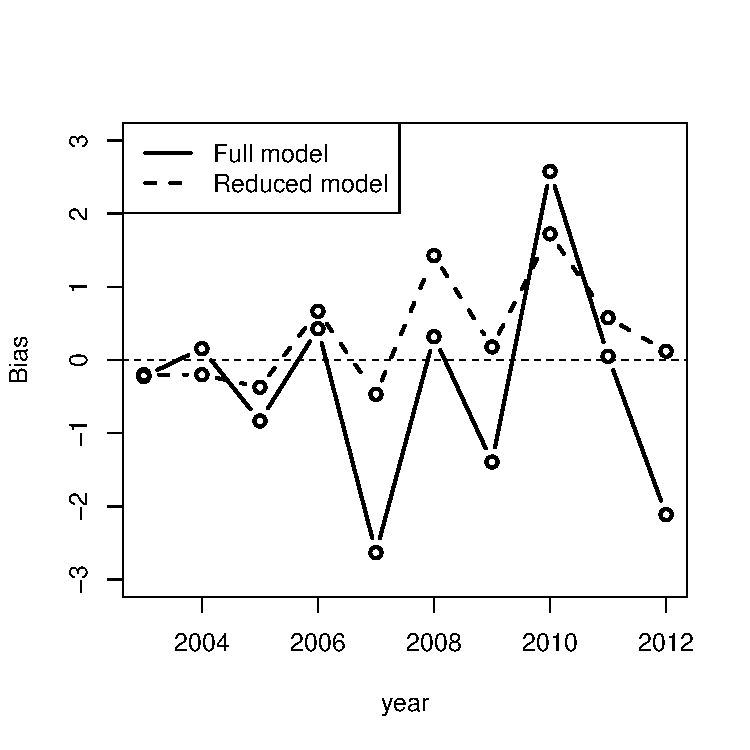
\includegraphics[width=0.32\textwidth]{Chapter-appli/rolling_predbias_full_vs_reduced_gamma.pdf}
	& 
		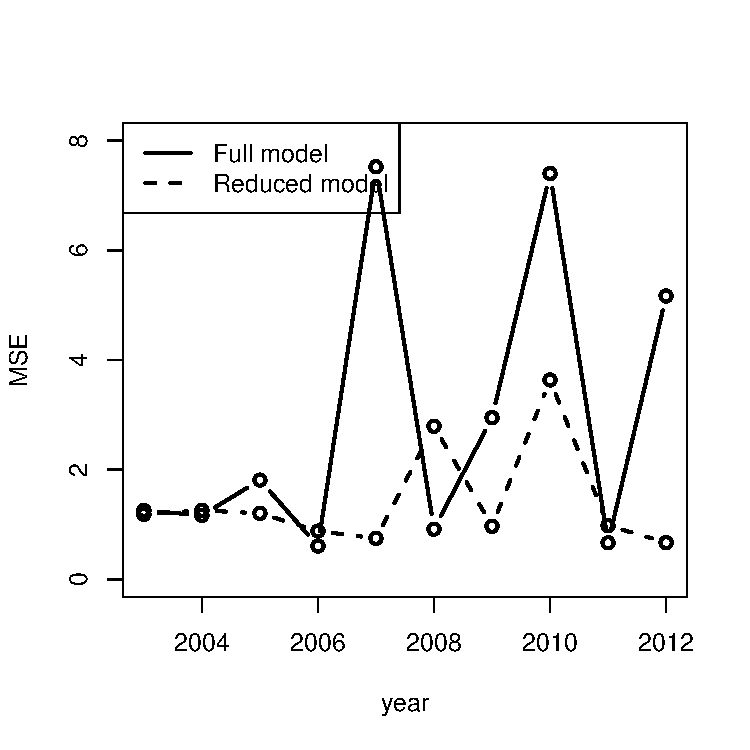
\includegraphics[width=0.32\textwidth]{Chapter-appli/rolling_predMSE_full_vs_reduced_gamma.pdf} \\
	(a) & (b) \\	
		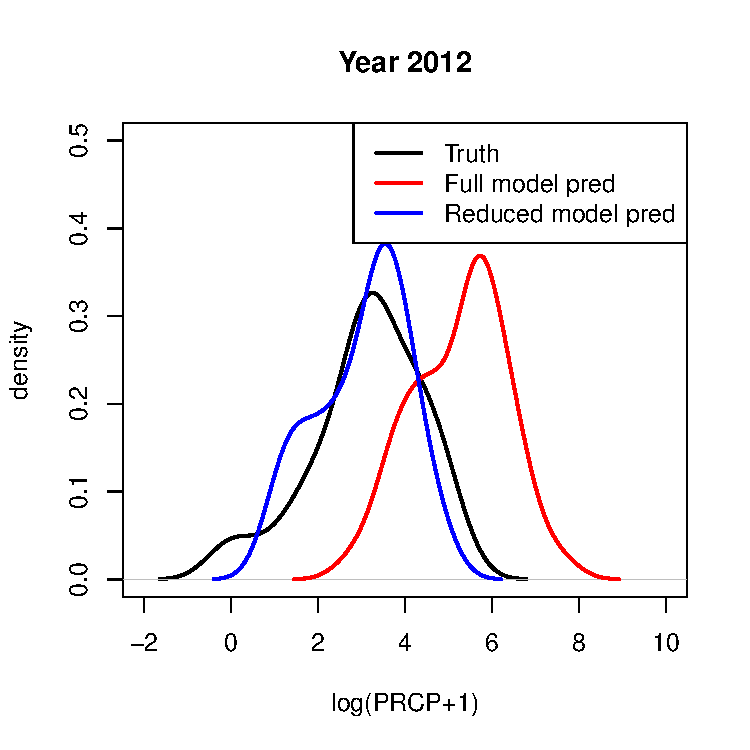
\includegraphics[width=0.32\textwidth]{Chapter-appli/rolling_density2012_full_vs_reduced_gamma.pdf}
	& 
		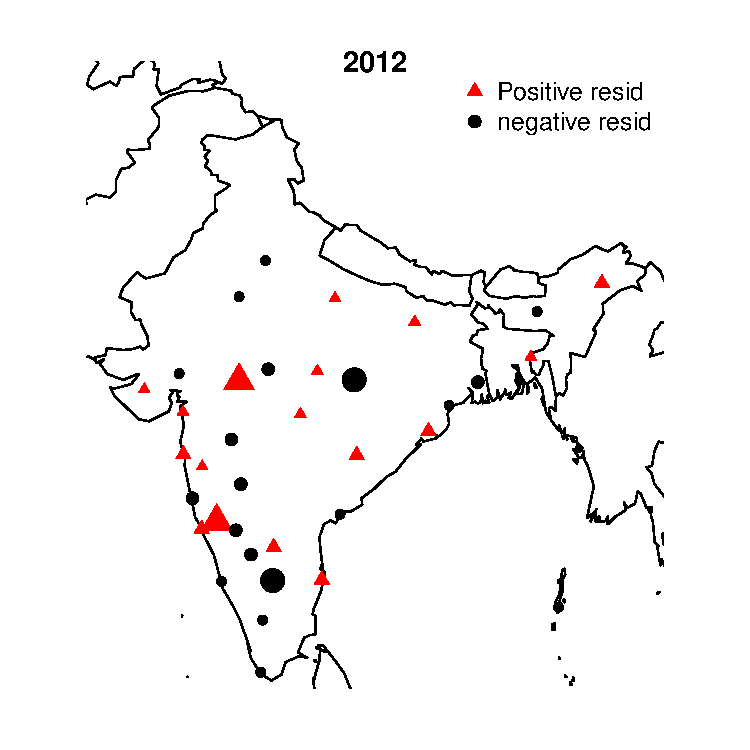
\includegraphics[width=0.32\textwidth]{Chapter-appli/rolling_map2012_full_vs_reduced_gamma.pdf} \\
	(c) & (d) \\	
\end{tabular}

\caption{Comparing full model rolling predictions with reduced models: (a) Bias across years, (b) MSE across years, (c) density plots for 2012, (d) stationwise residuals for 2012}
\label{fig:prepost}

\end{center}
\end{figure}

As a modeling step, we consider the  annual medians of all the above covariates as fixed effects, the log yearly rainfall at a weather station as response variable, and include year-specific random intercepts. \ref{table:raintable} lists the estimated $\hat{e} (\cS_{ -j})$ values in increasing order for the full model as well as all 35  models where a single variable is dropped. We implement the gamma bootstrap with Monte Carlo resample sizes $R = R_1 = 1000$. We use data until 2002 as training data, which contains $n=897$ samples. The mixed effects model trained on this data is evaluated for $\tau_n = n^\gamma; \gamma = 0.01, 0.02, \ldots, 0.16$. We take the covariate set corresponding to the tuning parameter which minimizes future fixed effect prediction errors on the testing data, i.e. for the period 2003-2012. Outputs of the fast $e$-value procedure for this covariate set are listed in \ref{table:raintable}. The variables listed above {\textit{none}} in this table are considered relevant by our $e$-value criterion.

All the variables selected by our procedure have documented effects on Indian monsoon \citep{KrishChapter, MoonWangHa12}. The single largest contributor is {\textit{maximum temperature}}, whose relation to  precipitation is based on the Clausius-Clapeyron relation is now classical knowledge in Physics. It seems 
that wind velocities high up in the atmosphere are not significant contributors, and the fact that many covariates are selected in the process highlights the complexity of the system.

%TA seems to have a large influence. Several MJO indices are selected when starting from a 
%full model with everything but TA, but are dropped in favor of TA when it is included in 
%the full model. The EPNP and the 120E index of MJO quantify intraseasonal oscillations in 
%sea-surfact temperature and troposhperic air circulation, respectively, and in our 
%analysis both get selected with very close values of $C_n$.

To check out-of-sample prediction performance of the estimated minimal adequate, we use a rolling validation scheme. For each of the 10 test years: 2003--2012, we select important variables from the model built on past 25 year's data (i.e. use data from 1978--2002 for 2003, 1979-2003 for 2004 and so on), build a model using them and compare predictions on test year obtained from this model with those from the full model. \ref{fig:prepost} summarizes results obtained through this process. Across all testing years, reduced model predictions have less bias as well as are more stable (panels a and b, respectively). The better approximations of truth by reduced models is also evident from the density plot for 2012 in panel c, and there does not seem to be any spatial patterns in its residuals as well (panel d).
%%%%% NOT TRUE PROBABLY
%\begin{Proposition}
%Given a sample size $n$ and any wrong conditional model $\mu^w = (\alpha^w, \bfbeta_c^w)$, there exists a correct conditional model $\mu^{wc} = (\alpha^{wc}, \bfbeta_c^{wc})$ so that $C_n(\mu^w) \leq C_n(\mu^{wc})$, .
%\end{Proposition}
%
%\begin{proof}
%$\bfbeta^w_c$ can be divided into two subvectors, by collecting its elements that actually belong to $\bfbeta$, and those that do not. Suppose $\alpha^w_0$ and $\alpha^w_1$ are the index sets corresponding to these subvectors, so that $\alpha^w = \alpha^w_0 \cup \alpha^w_1$. Since $\mu^w$ is a wrong model, $\alpha^w_1 \neq \emptyset$. Now take $\bfbeta^{wc}_c = \bfbeta(\alpha^w), \alpha^{wc} = \alpha^w$ and $\mu^{wc} = (\alpha^{wc}, \bfbeta^{wc}_c)$. For any estimate $\hat\bfbeta(\alpha^{wc})$, $\tilde\bfbeta(\mu^w)$ can be reached from $\tilde\bfbeta(\mu^{wc})$ by traveling sequentially along the coordinates in $\alpha^w_1$. The value of depth function decreases in each step because of upper level sets being convex. Finally, we shall have $D\left( \tilde\bfbeta_n(\mu^w), F_n \right) \leq  D\left( \tilde\bfbeta_n(\mu^{wc}), F_n \right)$, and hence $C_n(\mu^w) \leq C_n(\mu^{wc})$.
%\end{proof}
%%%%%

\section{Spatio-temporal Dependence Analysis in fMRI data}

In a second application, we apply our proposed method of model selection to analyze brain activity data obtained using functional Magnetic Resonance Imaging (fMRI). Typically, the brain is divided by a grid into three-dimensional array elements called voxels, and activity is measured at each voxel. More specifically, a series of three-dimensional images are obtained by measuring Blood Oxygen Level Dependent (BOLD) signals for a time interval as the subject performs several tasks at specific time points. A single fMRI image typically consists of voxels in the order of $10^5$, which makes even fitting the simplest of statistical models computationally intensive when it is repeated for all voxels to generate inference, e.g. investigating the differential activation of brain region in response to a task.

The dataset we work with comes from a recent study involving 19 test subjects and two types of visual tasks \citep{WakemanHenson15}. Each subject went through 9 runs, in which they were showed faces or scrambled faces at specific time points. In each run 210 images were recorded in 2 second intervals, and each 3D image was of the dimension of $64 \times 64 \times 33$, which means there were 135168 voxels. Here we use the data from a single run on subject 1, and perform a voxelwise analysis to find out the effect of time lags and BOLD responses at neighboring voxels on the BOLD response at a voxel. Formally we consider two  models at voxel $i \in \{1,2,...,V\}$ at a time point $t \in \{1,2,...,T\}$.

\subsection{Temporal model} The first model we consider is a $K$-th order autoregressive model in which we try to determine the effect of time lag upto 5 past frames on the BOLD response in voxel $i$ through the coefficients $(\delta_{i1},...,\delta_{i5})$:
%
$$ y_i(t) = x_{ia}(t) \beta_{ia} + x_{ib}(t) \beta_{ib} + \sum_{l=1}^q t^{l-1} \gamma_{il} + \sum_{K=1}^5 y_i(t-k) \delta_{i,t-k} + \epsilon_i(t)
$$
%
\noindent Here $x_{ia}(t)$ and $x_{ib}(t)$ are stimulus values corresponding to the two tasks at time $t$ and $\sum_{l=1}^q t^{l-1} \gamma_{il}$ is the polynomial drift terms to account for background noise. The stimulus values are calculated through a deterministic equation given the exact time points a face (stimulus $a$) or scrambled image (stimulus $b$) is shown \citep{EloyanEtal14}.

In this analysis we consider $K=5$ and $q=2$, i.e. an AR(5) model with quadratic drift. With this specification, a very small fraction of voxels had any neighbors selected with any autoregressive effects (less than 1\%), and most of them was in empty areas, indicating noise.

\subsection{Spatial model}
Our second model is a spatial regression model which tries to determine the amount of spatial dependence that exists between neighboring voxels. For this, apart from the two stimulus term and two drift terms, we consider BOLD responses at all the immediate neighbors of a voxel as potential predictors:
%
$$ y_i(t) = x_{ia}(t) \beta_{ia} + x_{ib}(t) \beta_{ib} + \sum_{l=1}^q t^{l-1} \gamma_{il} + \sum_{n \in N_i} y_n(t) \delta_{i,n} + \epsilon_i(t)
$$
%
Here $N_i$ is the set of neighbors of voxel $i$, $\delta_{i,n}$ is the coefficient corresponding to the effect of neighbor $n$ of voxel $i$. We consider only immediate neighbors of a voxel. In 3-dimensional space there are 26 such neighbors for voxel not at the periphery of the grid, so the total number of predictors in the voxelwise model in this case is 30. We exclude any voxel on the periphery of the $64 \times 64 \times 33$ grid from the analysis. We also consider the drift term to be quadratic as before. Further, since a very small fraction of voxels were positive for lag terms in the previous temporal model, we decided not to include any autoregressive term here.

Clubbing together the stimuli, drift terms and neighbor terms into a combined design matrix $\tilde \bfX = (\tilde \bfx(1)^T,...,\tilde \bfx(T)^T)^T$ and coefficient vector $\bftheta_i$, we can write $y_i(t) = \tilde \bfx(t)^T \bftheta_i + \epsilon_i(t) $. We now estimate the set of non-zero coefficients in $\bftheta_i$ using our method. Suppose this set is $R_i$, and its subsets containing coefficient corresponding to neighbor and non-neighbor (i.e. stimuli and drift) terms are $S_i$ and $T_i$, respectively. To quantify the effect of neighbors we now calculate the corresponding $F$-statistic:
%
$$
F_i = \frac{(\sum_{n \in S_i} \tilde x_{i,n} \hat\theta_{i,n})^2}{(y_i(t) - \sum_{n \in T_i} \tilde x_{i,n} \hat\theta_{i,n})^2} \frac{|n-T_i|}{|S_i|}
$$
and obtain its $p$-value, i.e. $P(F_i \geq F_{|S_i|,|n-T_i|})$.

\ref{fig:fmrifigure} shows plots of the voxels with a significant $p$-value from the above $F$-test. Both left and right visual cortex areas show high spatial dependence, although this is much higher on the left side. Signals from the right eye are processed by the left visual cortex, and high spatial dependence among voxels in both these areas suggest that the right eye was more involved in processing visual signals for this specific subject. We also notice activity in cerebellum, the role of which in visual perception is well-documented \citep{CalhounEtal10, Kirschen10}.

In terms of future work, we aim to expand on the encouraging findings of this study and repeat the procedure on other individuals in the study. An interesting direction here might be including subject specific random effects and correlating their clinical outcomes (if any) to the observed spatial dependency patterns in their brain.

\begin{figure}
\centering
\captionsetup{font=footnotesize}
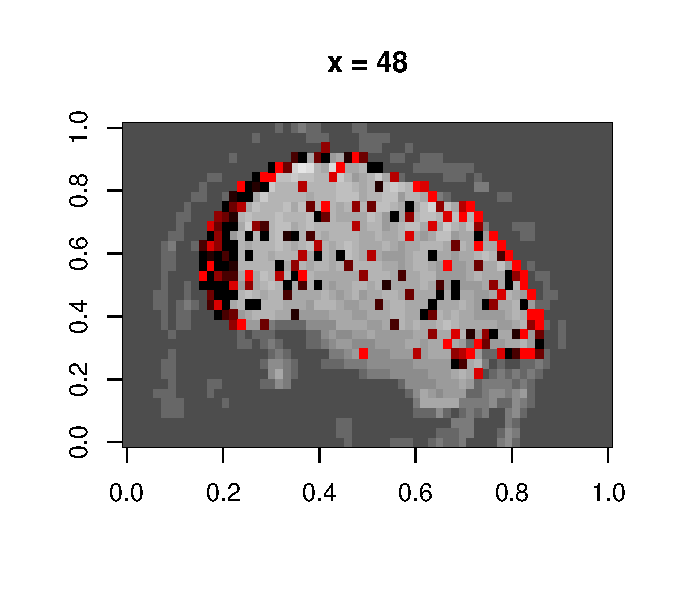
\includegraphics[width=.32\textwidth]{Chapter-appli/xslice}
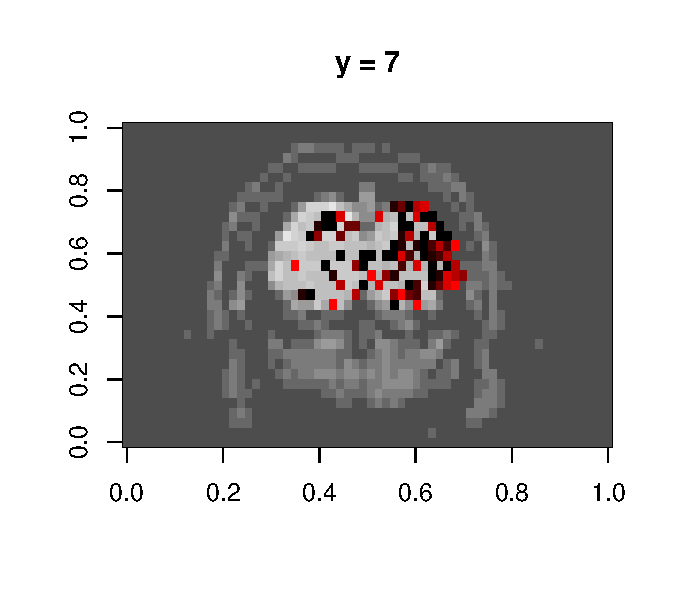
\includegraphics[width=.32\textwidth]{Chapter-appli/yslice}\\
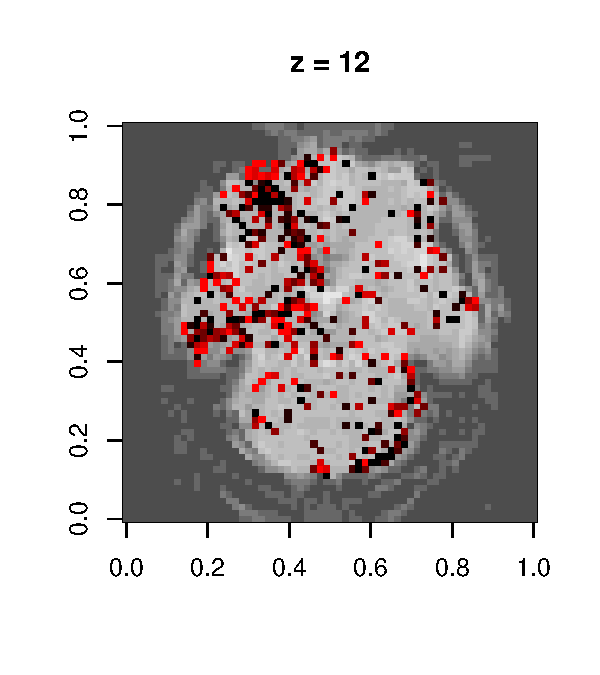
\includegraphics[width=.32\textwidth]{Chapter-appli/zslice}
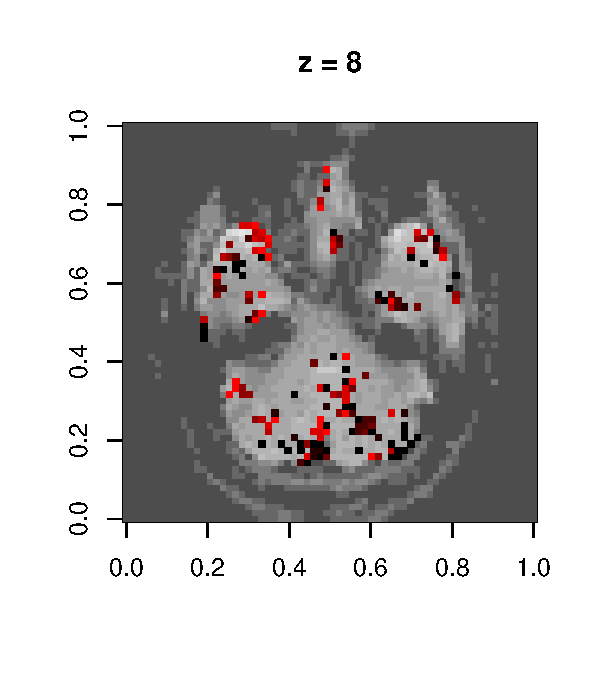
\includegraphics[width=.32\textwidth]{Chapter-appli/zslice2}\\
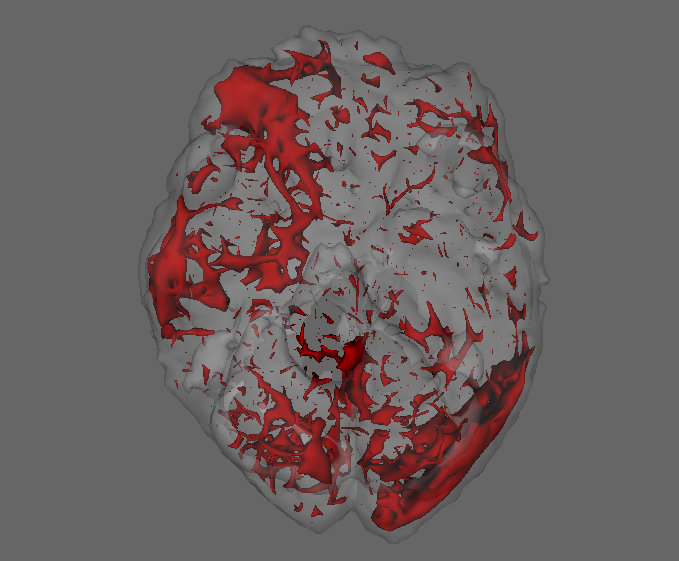
\includegraphics[width=.5\textwidth]{Chapter-appli/screenshot}

\caption{(Top) Plot of significant $p$-values at 95\% confidence level at the specified cross-sections; (bottom) a smoothed surface obtained from the $p$-values clearly shows high spatial dependence in right optic nerve, auditory nerves, auditory cortex and left visual cortex areas}
\label{fig:fmrifigure}
\end{figure}

\section{Selection of Important Single Nucleotide Polymorphisms behind behavioral traits from Familial Genome Wide Association Studies data}
\label{sec:TwinSection}

\subsection{Motivation}
Genome Wide Association Studies (GWAS), where genetic variants across the full human genome are analyzed, are becoming more and more relevant in recent years for the purpose of determining which of the variants are associated behind the expression of complex traits. The advent of efficient and economical genotyping technology enables researchers to scan the genome at hundreds of thousands of Single Nucleotide Polymorphisms (SNPs), and improvements in computational speed in the past few decades have helped in feasible analysis of the huge amount of data collected in order to detect significant associations \citep{VisscherEtal12}. One major challenge in such studies is the small effects individual SNPs have: detecting which requires large sample sizes \citep{ManolioEtal09}. For quantitative behavioral traits, for example alcohol dependence, drug abuse, Anorexia and depression, this problem is amplified because of the additional noise introduced by variation due to the environment the subject grew up in. This is one of the motivations of performing GWAS on families (GWAF) instead of unrelated individuals, through which the environmental variation can be reduced: so as to require smaller samples to detect the same magnitude of SNP effect. Another major reason, of course, of performing GWAS on familial data is to detect gene-environment interactions associated with development of behavioral traits. The data analyzed in such families typically consist of trait information and genotypes of from parents and their children, who can be either identical twins, non-identical twins or adpoted.

Single-marker tests, i.e. analyzing the effect of multiple SNPs separately on the quantitative phenotype and then selecting a group of SNPs by setting suitable thresholds on the resulting $p$-values, often after correction for multiple testing, is the most commonly used method to detect SNPs associated with the phenotype being studied. Although simultaneously estimating the fixed effect of a single SNP as well as the stratified population variance covariance matrix reflecting the familial structure, and repeating this for a large number of SNPs is a computationally prohibitive task, several fast approximation methods exist in the literature that tackle this while maintaining moderately high power. The GRAMMAR method of \cite{AulchenkoEtal07} and the association test of \cite{ChenAbecasis07} are examples of this. While these two methods are able to efficiently analyze GWAF data, they assume that phenotypic similarity within families is entirely due to their genetic similarity and ignore the effect of shared environment. In GWAF data from nuclear (i.e. unrelated) families, the proportion of phenotypic variation explained by the shared environmental effects is often substantial, sometimes as high as 51\% \citep{McGueEtal13} or 74\% \citep{DeNeveEtal13}: in which case such methods shall not be able to account for this added variation. To remedy this, \cite{LiEtal11} proposed a rapid method (RFGLS) that computes $p$-values corresponding to each SNP through a rapid approximation of the single-SNP generalized least squares model taking into account genetic and environmental sources of familial similarity.

A major issue with all such methods of single-marker analysis is that they are not always effective for detecting functionally relevant SNPs or regions in the genome. A single SNP is sometimes not enough to capture the extent of association \citep{YangEtal12, Ke12}. This includes cases when there are multiple causal SNPs closely located inside a gene in high Linkage Disequilibrium (LD) with one another. The causal SNP may even not be genotyped if its variants are unlikely to be present in the sample population (e.g. the variant of the SNP rs671 responsible for low alcohol tolerance in asians is rare in caucasians), and other SNPs highly correlated with it are genotyped instead.

%Due to the weak signal of individual SNPs as well as the heavy amount of correlation among them, detecting SNPs that are actually associated with the quantitative trait being analyzed is statistically challenging. A major impediment of estimating effects of multiple SNPs \textit{while} taking into account theirIn any kind of GWAS, fitting separate models on single markers typically suffer from loss of power.
% However the dependent data structure and large sample sizes in familial GWAS data calls for usage of suitable statistical models, for example mixed effet modelling, which makes even training a single model computationally intensive. and because of this any traditional variable selection approach is infeasible in such setup.

Here we propose to tackle this through fitting mixed effect models with the behavioral trait phenotype as respone and a group of SNPs (e.g. SNPs inside a single gene) as fixed effect predictors, and selecting important SNPs through a model selection approach. Although the major impediment of applying model selection techniques in GWAS setup is the high computational cost, some fast methods have been proposed that are able to perform SNP seletion from a multi-SNP model on GWAS data from \textit{unrelated individuals} \citep{ZhangEtal14,FrommeletEtal12}. However, these methods still rely on fitting models corresponding to multiple predictor sets. This makes them unsuitable to be adapted to the GWAF setup because of the much higher computational costs associated with training multiple mixed effect models that take into account within-family correlation between individuals, as compared to models that assume independent observations.

We shall use our $e$-values framework to provide a solution to this situation. As showed in the last chapter, our variable selection technique based on $e$-values requires only fitting the `full model': which makes it suitable to be utilized here.

\subsection{The MCTFR data}
The familial GWAS dataset collected and studied by Minnesota Center for Twin and Family Research (MCTFR)\citep{LiEtal11, MillerEtal12, McGueEtal13} consists of samples from three longitudinal studies conducted by the MCTFR: (1) the Minnesota Twin Family Study (MTFS: \cite{IaconoEtal99}) that covers twins and their parent, (2) the Sibling Interaction and Behavior Study (SIBS: \cite{McGueEtal07}) that includes adopted and biological sibling pairs and their parents, and (3) the enrichment study (ES: \cite{KeyesEtal09}) that extended the MTFS by oversampling 11 year old twins who are highly likely to develop substance abuse. While 9827 individuals completed the initial assessments for participation in the study, after several steps of screening the final sample consisted of 7188 caucasian individuals clustered in 2300 nuclear families. %Here a total of 7188 Caucasian individuals, who come from $\sim 2300$ families, have been genotyped. A detailed description of the data is available at \cite{MillerEtal12}.

DNA samples collected from the subjects were analyzed using Illumina’s Human660W-Quad Array for 561,490 non-intensity SNP markers. After several data cleaning steps for quality control, 527,829 SNPs were retained. Covariates for each sample included age, sex, birth year, generation (parent or offspring), as well as two-way interactions between generation and other three covariates each. As for the quantitative phenotypes, five of them were studied in this GWAS: (1) Nicotine dependence, (2) Alcohol consumption, (3) Alcohol dependence, (4) Illegal drug usage, and (5) Behavioral disinhibition. The response variables corresponding to these phenotypes were derived from questionnaires using a hierarchical approach based on factor analysis \citep{HicksEtal11}.

A more detailed description of the data is available  in \cite{MillerEtal12}. Several studies have been performed that focus on different aspects of this dataset. \cite{LiEtal11} used RFGLS to single out causal SNPs behind the height of participants, while \cite{McGueEtal13} used the same method to study SNPs behind the development of all five indicators of behavioral disinhibition mentioned above. \cite{IronsThesis12} focused on the effect of several factors affecting alcohol use in the study population, namely the effects of polymorphisms in the ALDH2 gene and the GABA system genes, as well as the effect of early exposure to alcohols as adolescents to adult outcomes. Finally \cite{CoombesThesis16} used a bootstrap-based combination test and a sequential score test to evaluate gene-environment interactions behind phenotypic outcomes in the data.

\subsection{Statistical model}
We shall demonstrate the use of $e$-values in this context using a Linear Mixed Model (LMM) framework. We assume that the families modeled are unrelated to one another, i.e. they are nuclear pedigrees. We stick to this structure for ease of representation, although as discussed shortly, the model fitting process remains unchanged for larger pedigrees.

We assume there are a total of $m$ families, with the $i$-th pedigree containing $n_i$ individuals. Denote by $\bfy_i = (y_{i 1}, \ldots, y_{i n_i})^T $ the quantitative trait values for individuals in that pedigree, while the matrix $\bfG_i \in \BR^{ n_i \times p_s}$ containing their genotypes for a bunch of SNPs. Let $\bfC_i \in \BR^{ n_i \times p}$ denote the data on $p$ covariates for individuals in the pedigree $i$. Given these, we consider the following model.
%
\begin{align}\label{eqn:LMMeqn}
\bfY_i = \alpha + \bfG_i \bfbeta_g + \bfC_i \bfbeta_c + \bfepsilon_i
\end{align}
%
with $\alpha$ the intercept term, $\bfbeta_g$ and $\bfbeta_c$ fixed coefficient terms corresponding to the multiple SNPs and covariates, respectively, and $\bfepsilon_i \sim \cN_{n_i} (\bfZero, \bfV_i)$ the random error term. To account for the within-family dependency structure, we break up the random error variance into three independent components:
%
\begin{align}\label{eqn:partsOfV}
\bfV_i = \sigma_a^2 \bfPhi_i + \sigma_c^2 {\bf 1} {\bf 1}^T + \sigma_e^2 \bfI_{n_i}
\end{align}
%
The first part represents a within-family random effect term to account for effects of other SNPs. The matrix $\bfPhi_i$ is the relationship matrix within the $i$-th pedigree. Its $(s,t)$-th element represents two times the kinship coefficient, which is the probability that given that a random gene is drawn each from individuals $s$ and $t$ in pedigree $i$, these genes are `identical by descent', i.e. come from same common ancestor. The second part accounts for shared environmental effect within the family, while the third term finally quantifies other sources of variation unique to an individual.

Following basic probability, the kinship coefficient of a parent-child pair is 1/4, a full sibling pair or non-identical (or dizygous = DZ) twins is 1/4, and for identical (or monozygous = MZ) twins is 1/2 in a nuclear pedigree. Following this, we can construct the $\bfPhi_i$ matrices for different types of families:
%
\begin{align*}
\bfPhi_{MZ} = \begin{bmatrix}
1 & 0 & 1/2 & 1/2 \\
0 & 1 & 1/2 & 1/2 \\
1/2 & 1/2 & 1 & 1\\
1/2 & 1/2 & 1 & 1
\end{bmatrix},
\bfPhi_{DZ} = \begin{bmatrix}
1 & 0 & 1/2 & 1/2 \\
0 & 1 & 1/2 & 1/2 \\
1/2 & 1/2 & 1 & 1/2\\
1/2 & 1/2 & 1/2 & 1
\end{bmatrix},
\bfPhi_{Adopted} = \bfI_4
\end{align*}
%
for families with parents (indices 1 and 2) and MZ twins, DZ twins, or two adapted children (indices 3 and 4), respectively.

We use the R package \texttt{regress} to fit the above model with additive error structure. The package requires specifying the dependency structure of all samples in the data. For ease of representation, we only consider nuclear pedigrees with MZ twins in our simulation study and data analysis, which simplifies the overall relationship matrix $\bfPhi = \text{diag} ( \bfPhi_1, \ldots, \bfPhi_m)$ as $\bfI_m \otimes \bfPhi_{MZ}$. Note that, situations in which the pedigree structure is not nuclear can be readily handled in this situation by supplying the overall $\bfPhi$ matrix. The second overall structural component will be  $\bfI_m \otimes {\bf 1} {\bf 1}^T$. The \texttt{regress} procedure includes the third structure in \ref{eqn:partsOfV} by default.

\subsection{A conditional $e$-value}
We now take a closer look at the evaluation map distributions corresponding to reduced model coefficient estimates, in order to better detect the weak signals we are dealing with here and reduce the number of false positives. Carrying over notations from \ref{chapter:Chapter-evalue}, recall that the model formed by dropping the $j$-the index is denoted by $\cM_{-j}$, and we are going to inspect $\BD_{-j}$, the distribution of $D( \hat \bfbeta_{-j}, [\hat \bfbeta] ) $ by comparing it with $\BD :=$ distribution of $D( \hat \bfbeta, [\hat \bfbeta] ) $. Also define by $\mu(.)$ the mean operator on the corresponding distributions.

Recall from \ref{chapter:Chapter-evalue} that we approximate the above distributions and the final $e$-value through resampling. The quality of approximation depends on the variance parameter $\tau_n^2$, and as seen in the simulation section, on the type of bootstrap scheme used (moon/ gamma/ generalized). Because of the high-computational overhead of the \texttt{regress} procedure, we shall use the parametric generalized bootstrap scheme here. We would also like to emphasize that all observations in this subsection are entirely empirical and from controlled simulation setups, and further studies are warranted to theoretically characterize such behavior.

We denote by $\hat \BD_{-j} (\tau)$ and $\hat\BD (\tau)$ the approximations of $\BD_{-j}$ and $\BD$, respectively, using a generalized bootstrap scheme with standard deviation $\tau_n \equiv \tau$. According to theorem \ref{Theorem:ModelScore}, in case $\BD_{-j}$ is an inadequate model distribution, the mean of $\hat \BD_{-j} (\tau)$ goes to 0 in probability for an intermediate rate of the bootstrap standard deviation. As $\tau$ increases, all reduced model distributions approach $\hat\BD (\tau)$. However, depending on the magnitude of signals at the non-zero indices, we observe that this behavior follows two different regimes. We demonstrate this using the simulation setup we elaborate on later in the chapter. In the plots below, $h$ represents the relative magnitude of non-zero entries in the coefficient vector: for which we consider two choices, $h=5$ and $h=0.05$.

\begin{figure}
\centering
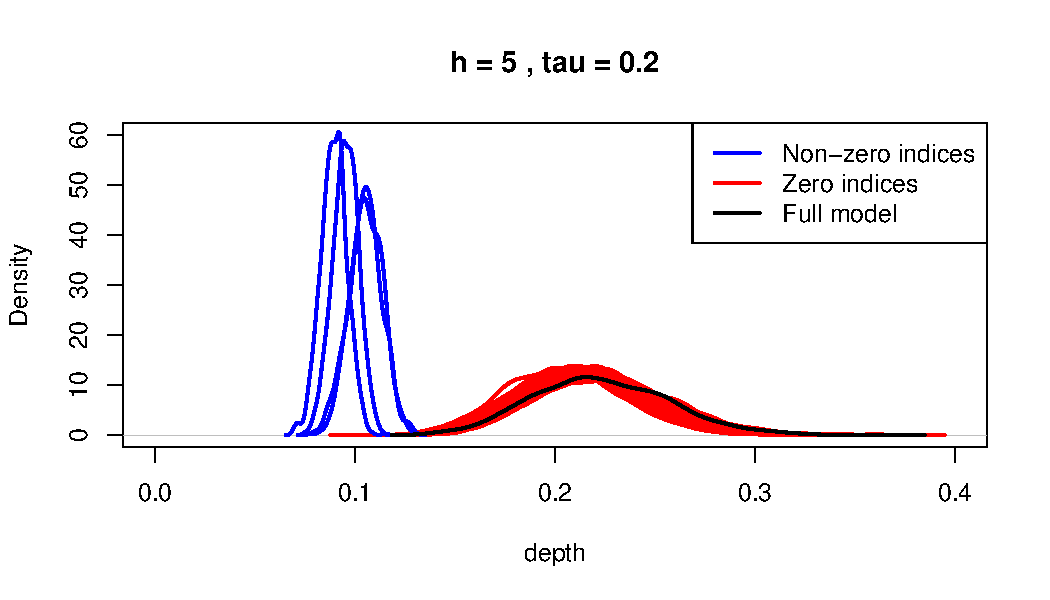
\includegraphics[height=.22\textheight]{Chapter-appli/plot_h5_tau2}\\
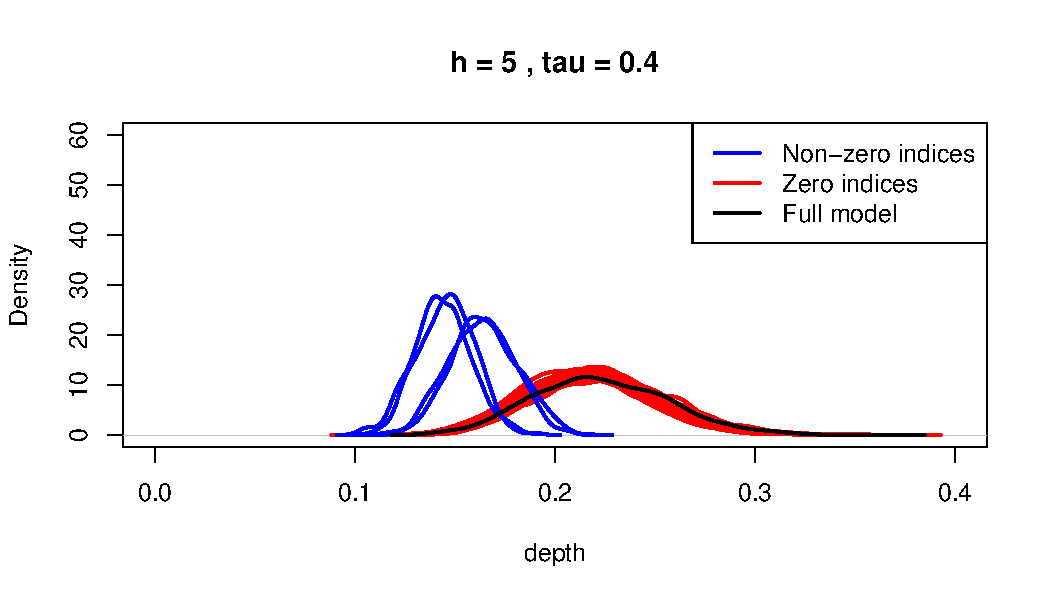
\includegraphics[height=.22\textheight]{Chapter-appli/plot_h5_tau4}\\
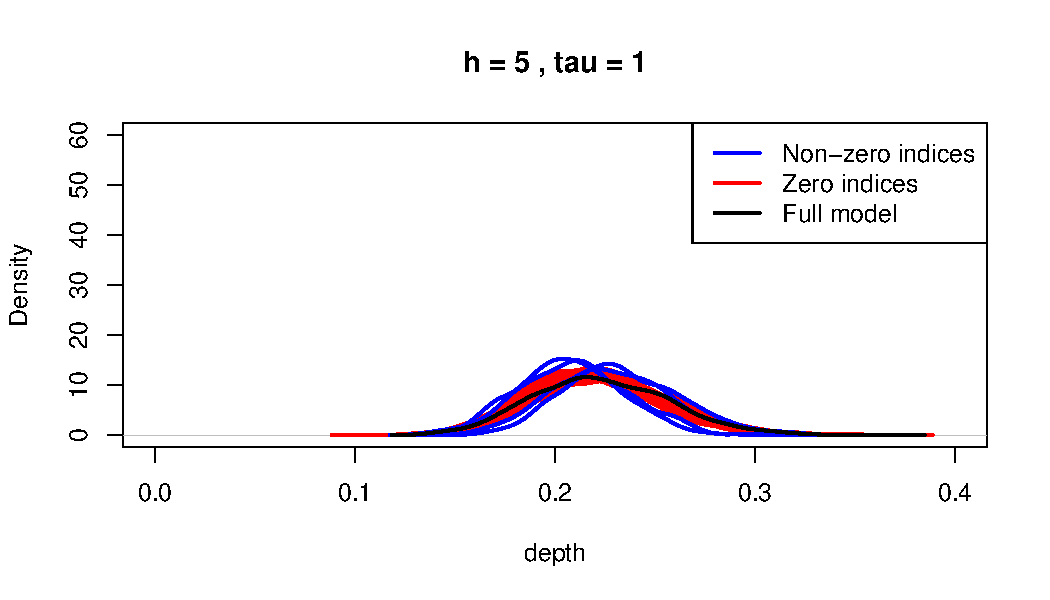
\includegraphics[height=.22\textheight]{Chapter-appli/plot_h5_tau10}\\
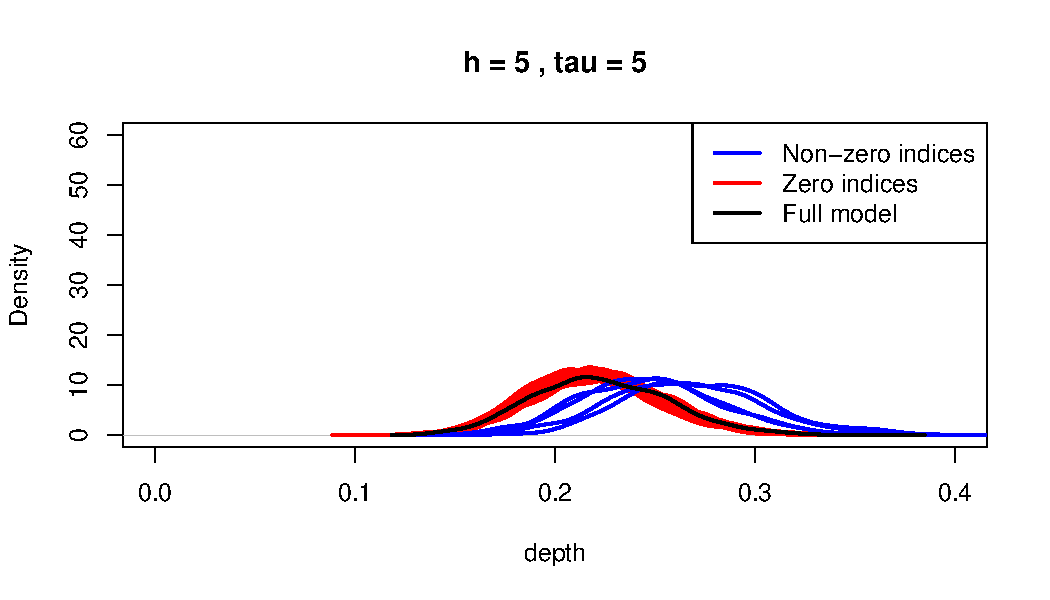
\includegraphics[height=.22\textheight]{Chapter-appli/plot_h5_tau50}
\caption{Density plots for $\hat \BD(\tau)$ and $\hat \BD_{-j}(\tau)$ for all $j$ in simulation setup, with signal parameter $h=5$ and bootstrap standard deviations $\tau = 0.2, 0.4, 1, 5$}
\label{fig:figLargeTau1}
\end{figure}

\begin{figure}
\centering
\includegraphics[height=.22\textheight]{{"Chapter-appli/plot_h0.05_tau2"}.pdf}\\
\includegraphics[height=.22\textheight]{{"Chapter-appli/plot_h0.05_tau4"}.pdf}\\
\includegraphics[height=.22\textheight]{{"Chapter-appli/plot_h0.05_tau10"}.pdf}\\
\includegraphics[height=.22\textheight]{{"Chapter-appli/plot_h0.05_tau50"}.pdf}
\caption{Density plots for $\hat \BD(\tau)$ and $\hat \BD_{-j}(\tau)$ for all $j$ in simulation setup, with signal parameter $h=0.05$ and bootstrap standard deviations $\tau = 0.2, 0.4, 1, 5$}
\label{fig:figLargeTau2}
\end{figure}

\paragraph{(a) Large signal regime ($h=5$: \ref{fig:figLargeTau1})} When $\BD_{-j}$ corresponds to an inadequate model, i.e. the $j$-th coefficient of the true parameter vector is non-zero, for small values of $\tau$ we can clearly distinguish this distribution from that of $\hat\BD (\tau)$ in their density plots. As $\tau$ increases, the inadequate model distributions seem to have more and more positive bias. However, when $j$ is a non-essential covariate, the reduced distributions are close to $\hat \BD(\tau)$ for all values of $\tau$.

\paragraph{(b) Small signal regime ($h=0.05$: \ref{fig:figLargeTau2})} When the actual signal in $\beta_j$ is weak, the inadequate reduced model distributions still approach $\hat \BD(\tau)$ as $\tau$ goes up but stabilize at the full model distribution instead of passing it for very large $\tau$ ($\tau=5$ here). However the adequate model distributions seem to exhibit a similar behavior: albeit staying to the left of inadequate model density plots in general.

This increased ambiguity of reduced model distributions for small signals make it difficult to distinguish between two types of model distributions using the mean operator, which ends up being very conservative in the second case. For this reason we consider the usage of a different summarizing function that will be able to capture the differentiate between the two types of reduced model distributions across a broader range of the signal-to-noise ratio, specifically by setting a lower detection threshold than the same operator on the full model distribution. Here we focus on a specific alternate formulation of the $e$-value that is based on a tail quantile of $\hat \BD_{-j} (\tau)$:
%
\begin{align}
e_q (\cM_{-j} | \tau) = q \text{-th quantile of } \hat \BD_{-j} (\tau)
\end{align}
%
for some fixed $q \in (0,1)$. Notice that for any $q$, the quantity $e_q (\cM_{-j} | \tau)$ is conditional on the bootstrap standard deviation parameter $\tau$.

The motivation behind this is the observation that the inadequate and adequate model distributions have different tail behaviors for intermediate values of $\tau$, and setting an appropriate upper threshold to tail probabilities for a suitable fixed quantile of these distributions with respect to $\hat \BD(\tau)$ can possibly separate out the two types of distributions. The choice of threshold potentially depends on several factors such as the value of $q$, the statistical model used, degree of sparsity of parameters in the data generating process. In the following section we shall experiment with different thresholds to illustrate this.
Also note that we still retain the main flavor of the $e$-values method, by training only the full model and then use Monte Carlo resampling to compute $e_q (\cM_{-j} | \tau)$ for all $j$ and a range of $\tau$.

\subsection{Simulation}
\label{sec:SimSection}

We now compare the performance of the above formulation of quantile $e$-values in a simulation setup. For this, consider the model in \ref{eqn:LMMeqn} with no environmental covariates. We consider familes with MZ twins and first generate the covariate matrices $\bfG_i$. We take a total of $p_g = 50$ SNPs, and to simulate correlation among SNPs in the genome generate them in correlated blocks of 6, 4 ,6, 4 and 30. We set the correlation between two SNPs inside a block at 0.7, and consider the blocks to be uncorrelated. For each parent we generate two independent vectors of length 50 with the above correlation structure, and entries within each block being 0 or 1 following Bernoulli distributions with probabilities 0.2, 0.4, 0.4, 0.25 and 0.25 (Minor Allele Frequency or MAF) for SNPs in the 5 blocks, respectively. The genotype of a person is then determined by taking the sum of these two vectors: thus entries in $\bfG_i$ can take the values 0, 1 or 2. Finally we set the common genotype of the twins by randomly choosing one allele vector from each of the parents and taking their sum.

We repeat the above process for $m=250$ families. In GWAS there are generally a small number of causal SNPs, each explaining small proportions of the overall variability in response variable. To reflect this in our simulation setup, we assume that the first entries in each of the first four blocks above are causal, and each of them explains $h/(\sigma_a^2+\sigma_c^2+\sigma_e^2) \%$ of the overall variability. The term $h$ is known as the \textit{heritability} of the corresponding SNP (and can of course vary across SNPs). The value of the non-zero coefficient in $k$-th group: $k = 1, ..., 4$, say $\beta_k$ is calculated using the formula:
%
\begin{align}
\beta_k = \sqrt{ \frac{h}{(\sigma_a^2+\sigma_c^2+\sigma_e^2). 2 \text{MAF}_k (1 - \text{MAF}_k) }}
\end{align}
%
We fix the following values for the error variance components: $\sigma_a^2 = 4, \sigma_c^2 = 1, \sigma_e^2 = 1$, and generate pedigree-wise response vectors $\bfy_1, \ldots, \bfy_{250}$ using the above setup. To consider different SNP effect sizes, we repeat the above setup for $h \in \{10, 5, 2, 1, 0 \}$, generating 1000 datasets for each value of $h$.

\subsubsection{Methods and metrics}
For this simulated data, we compare our $e$-value based approach with two other methods:

\paragraph{(1) Model selection on linear model:} Here we ignore the dependency structure within families by training linear models on the simulated data and selecting SNPs with non-zero effects by backward deletion using a modification of the BIC called mBIC2. This has been showed to give better results than single-marker analysis in GWAS for unrelated individuals \citep{FrommeletEtal12} and provides approximate False Discovery Rate (FDR) control at level 0.05 \citep{BogdanEtal11}.

\paragraph{(2) Single-marker mixed model:} We train single-SNP versions of \ref{eqn:LMMeqn} using a fast approximation of the Generalized Least Squares procedure (named Rapid Feasible Generalized Least Squares or RFGLS: \cite{LiEtal11}), obtain marginal $p$-values from corresponding $t$-tests and use the Benjamini-Hochberg (BH) procedure to select significant SNPs at FDR = $0.05$.

\vspace{1em}\noindent We compute the $e$-values by setting projection depth \citep{zuo03} as the evaluation function. With the $e$-value being the $q$-th quantile of the evaluation map distribution, we set the detection threshold value at the $t$-th multiple of $q$ for some $0 < t < 1$. This means all indices $j$ such that $q$-th quantile of the bootstrap approximation of $\hat \BD_{-j} (\tau)$ is less than the $tq$-th quantile of $\hat \BD (\tau)$ will get selected as the set of active predictors. We repeat the $e$-value procedure for different values of the bootstrap standard deviation $s \in \{ 0.3, 0.35, \ldots, 0.95, 2 \}$. Consequently, we take as the final estimated set of SNPs the SNP set $\hat \cS (\tau)$ that minimizes fixed effect prediction error (PE) on an independently generated test dataset $\{ (\bfy_{test,i}, \bfG_{test,i}), i = 1, \ldots, 250 \}$ from the same setup above:
%
\begin{align*}
& \text{PE} (\tau | q,t)  = \sum_{i=1}^{250} \sum_{j=1}^4 \left( y_{test,ij} - \bfg_{test,ij}^T \hat \bfbeta_{\hat \cS (\tau)} \right)^2; \\
& \hat \cS_0 (q,t) = \argmin_\tau \text{PE} (\tau | q,t)
\end{align*}

The metrics to evaluate each method we implement are:

\begin{enumerate}
\item True Positive (TP): proportion of causal SNPs detected;

\item True Negative (TN): proportion of non-causal SNPs undetected;

\item Relaxed True Positive (TPR): proportion of detecting any SNP in each of the 4 blocks with causal SNPs, i.e. for the selected index set $\hat \cS_0 (q,t)$,
%
$$
\text{TPR} ( \hat \cS_0 (q,t) ) = \frac{1}{4} \sum_{i=1}^4 \BI ( \text{Block } i \cap \hat \cS_0 (q,t) \neq \emptyset )
$$
%

\item Relaxed True Negative (TNR): proportion of SNPs in block 5 undetected.
\end{enumerate}

\noindent We consider the third and fourth metrics to cover situations in which the causal SNP is not detected itself, but highly correlated SNPs with the causal SNP are. This is common in GWAS. Finally, we average all the above proportions over 1000 replications, and repeat the process for $ q \in \{ 0.9, 0.5, 0.2, 0.1 \}; t \in \{ 0.8, 0.7, 0.6, 0.5 \}$.

%Although the first two heritability values are larger compared to a typical GWAS setup, we use this setup to demonstrate limitations of the existing methodology even in a vastly simplified setting.

\subsubsection{Results}
% latex table generated in R 3.3.2 by xtable 1.8-2 package
% Sun Apr 16 18:24:09 2017
% latex table generated in R 3.3.2 by xtable 1.8-2 package
% Sun Apr 16 18:24:48 2017
\begin{table}
\begin{footnotesize}
\centering
    \begin{tabular}{c|c|c|c|cccc}
    \hline
     6x   & mBIC2       & RFGLS  & \multicolumn{5}{|c}{quantile $e$-values}    \\\cline{4-8}
    Heritability    &           & +BH		 & $q$    & $t=0.8$     & $t=0.7$     & $t=0.6$     & $t=0.5$     \\ \hline
    ~    & ~         & ~         & 0.9      & 0.95/0.97 & 0.95/0.97 & 0.95/0.98 & 0.94/0.98 \\
    $h=10$ & 0.79/0.99 & 0.95/0.92 & 0.5      & 0.96/0.97 & 0.96/0.98 & 0.95/0.98 & 0.94/0.98 \\
    ~    & ~         & ~         & 0.2      & 0.96/0.94 & 0.96/0.97 & 0.95/0.97 & 0.95/0.98 \\\hline
    ~    & ~         & ~         & 0.9      & 0.72/0.95 & 0.7/0.96  & 0.69/0.96 & 0.66/0.97 \\
    $h=5$  & 0.41/0.99 & 0.62/0.97 & 0.5      & 0.78/0.94 & 0.75/0.94 & 0.72/0.95 & 0.71/0.96 \\
    ~    & ~         & ~         & 0.2      & 0.83/0.91 & 0.78/0.94 & 0.75/0.95 & 0.73/0.95 \\\hline
    ~    & ~         & ~         & 0.9      & 0.26/0.97 & 0.24/0.97 & 0.23/0.98 & 0.21/0.98 \\
    $h=2$  & 0.11/0.99 & 0.14/0.99 & 0.5      & 0.34/0.95 & 0.28/0.96 & 0.27/0.97 & 0.26/0.97 \\
    ~    & ~         & ~         & 0.2      & 0.46/0.91 & 0.34/0.95 & 0.3/0.96  & 0.27/0.96 \\\hline
    ~    & ~         & ~         & 0.9      & 0.12/0.98 & 0.1/0.98  & 0.09/0.99 & 0.08/0.99 \\
    $h=1$  & 0.05/0.99 & 0.04/0.99    & 0.5      & 0.16/0.96 & 0.13/0.97 & 0.12/0.97 & 0.11/0.98 \\
    ~    & ~         & ~         & 0.2      & 0.25/0.93 & 0.16/0.96 & 0.13/0.97 & 0.13/0.97 \\\hline
    ~    & ~         & ~         & 0.9      & --/0.99 & --/0.99 & --/0.99 & --/0.99    \\
    $h=0$  & --/0.99 & --/0.99       & 0.5      & --/0.98 & --/0.98 & --/0.99 & --/0.99 \\
    ~    & ~         & ~         & 0.2      & --/0.94 & --/0.98 & --/0.98 & --/0.99 \\\hline
    \end{tabular}
    \caption{Average True Positive (TP) and True Negative (TN) proportions over 1000 replications for all three methods}
    \label{table:SNPSimTable0}
\end{footnotesize}
\end{table}

%% latex table generated in R 3.3.2 by xtable 1.8-2 package
%% Sun Apr 16 18:24:09 2017
%% latex table generated in R 3.3.2 by xtable 1.8-2 package
%% Sun Apr 16 18:24:48 2017
%\begin{table}
%\begin{footnotesize}
%\centering
%    \begin{tabular}{c|c|c|c|cccc}
%    \hline
%    6x    & mBIC2       & RFGLS  & \multicolumn{5}{|c}{quantile $e$-values}    \\\cline{4-8}
%    Heritability    &           & +BH		 & $q$    & $t=0.8$     & $t=0.7$     & $t=0.6$     & $t=0.5$     \\ \hline
%     ~    & 0.27/0.98 & 0.96/0.99 & 0.9      & 0.95/0.97 & 0.95/0.97 & 0.94/0.97 & 0.94/0.98 \\
%    ~    & ~         & ~         & 0.5      & 0.98/0.96 & 0.97/0.97 & 0.96/0.97 & 0.96/0.97 \\
%    h=10 & ~         & ~         & 0.2      & 0.99/0.9  & 0.97/0.96 & 0.97/0.97 & 0.96/0.97 \\
%    ~    & ~         & ~         & 0.1      & 0.99/0.83 & 0.98/0.93 & 0.97/0.96 & 0.96/0.97 \\
%    ~    & ~         & ~         & 0.05     & 0.99/0.74 & 0.98/0.88 & 0.97/0.94 & 0.97/0.96 \\ \hline
%    ~    & 0.16/0.98 & 0.63/0.99 & 0.9      & 0.74/0.95 & 0.73/0.95 & 0.71/0.96 & 0.69/0.97 \\
%    ~    & ~         & ~         & 0.5      & 0.83/0.93 & 0.78/0.94 & 0.76/0.95 & 0.75/0.95 \\
%    h=5  & ~         & ~         & 0.2      & 0.9/0.87  & 0.83/0.93 & 0.79/0.94 & 0.76/0.95 \\
%    ~    & ~         & ~         & 0.1      & 0.93/0.79 & 0.86/0.9  & 0.81/0.93 & 0.78/0.94 \\
%    ~    & ~         & ~         & 0.05     & 0.95/0.72 & 0.88/0.86 & 0.83/0.91 & 0.79/0.93 \\ \hline
%    ~    & 0.09/0.98 & 0.16/1    & 0.9      & 0.32/0.96 & 0.29/0.97 & 0.27/0.97 & 0.24/0.98 \\
%    ~    & ~         & ~         & 0.5      & 0.45/0.94 & 0.34/0.96 & 0.32/0.96 & 0.3/0.97  \\
%    h=2  & ~         & ~         & 0.2      & 0.66/0.86 & 0.47/0.93 & 0.38/0.95 & 0.33/0.96 \\
%    ~    & ~         & ~         & 0.1      & 0.77/0.79 & 0.57/0.9  & 0.43/0.94 & 0.37/0.95 \\
%    ~    & ~         & ~         & 0.05     & 0.82/0.71 & 0.64/0.85 & 0.5/0.92  & 0.41/0.94 \\ \hline
%    ~    & 0.07/0.98 & 0.05/1    & 0.9      & 0.16/0.97 & 0.14/0.98 & 0.13/0.98 & 0.11/0.99 \\
%    ~    & ~         & ~         & 0.5      & 0.26/0.95 & 0.18/0.97 & 0.17/0.97 & 0.15/0.98 \\
%    h=1  & ~         & ~         & 0.2      & 0.5/0.88  & 0.28/0.94 & 0.2/0.96  & 0.17/0.97 \\
%    ~    & ~         & ~         & 0.1      & 0.65/0.79 & 0.4/0.91  & 0.26/0.95 & 0.2/0.97  \\
%    ~    & ~         & ~         & 0.05     & 0.73/0.71 & 0.51/0.86 & 0.35/0.92 & 0.24/0.95 \\ \hline
%    ~    & 0.05/0.98 & 0.01/1    & 0.9      & 0.04/0.98 & 0.04/0.99 & 0.03/0.99 & 0.03/0.99 \\
%    ~    & ~         & ~         & 0.5      & 0.1/0.97  & 0.05/0.98 & 0.04/0.98 & 0.04/0.98 \\
%    h=0  & ~         & ~         & 0.2      & 0.32/0.89 & 0.1/0.96  & 0.06/0.98 & 0.05/0.98 \\
%    ~    & ~         & ~         & 0.1      & 0.5/0.82  & 0.22/0.93 & 0.1/0.97  & 0.06/0.98 \\
%    ~    & ~         & ~         & 0.05     & 0.64/0.73 & 0.37/0.87 & 0.2/0.94  & 0.09/0.97 \\ \hline
%    \end{tabular}
%    \caption{Average Relaxed True Positive (TPR) and Relaxed True Negative (TNR) proportions over 1000 replications for all three methods}
%    \label{table:SNPSimTable1}
%\end{footnotesize}
%\end{table}
\begin{table}
\begin{footnotesize}
\centering
    \begin{tabular}{c|c|c|c|cccc}
    \hline
    6x    & mBIC2       & RFGLS  & \multicolumn{5}{|c}{quantile $e$-values}    \\\cline{4-8}
    Heritability    &           & +BH		 & $q$    & $t=0.8$     & $t=0.7$     & $t=0.6$     & $t=0.5$     \\ \hline
    ~    & ~         & ~         & 0.9      & 0.96/0.97 & 0.96/0.97 & 0.95/0.98 & 0.94/0.98 \\
    $h=10$ & 0.84/0.99 & 0.96/0.99 & 0.5      & 0.96/0.97 & 0.96/0.97 & 0.95/0.98 & 0.95/0.98 \\
    ~    & ~         & ~         & 0.2      & 0.97/0.95 & 0.96/0.97 & 0.96/0.97 & 0.95/0.98 \\\hline
    ~    & ~         & ~         & 0.9      & 0.73/0.95 & 0.71/0.95 & 0.7/0.96  & 0.67/0.97 \\
    $h=5$  & 0.48/0.99 & 0.64/0.99 & 0.5      & 0.79/0.93 & 0.76/0.94 & 0.73/0.95 & 0.72/0.95 \\
    ~    & ~         & ~         & 0.2      & 0.85/0.91 & 0.79/0.93 & 0.76/0.94 & 0.74/0.95 \\\hline
    ~    & ~         & ~         & 0.9      & 0.29/0.96 & 0.27/0.97 & 0.25/0.98 & 0.23/0.98 \\
    $h=2$  & 0.16/0.99 & 0.16/0.99    & 0.5      & 0.37/0.95 & 0.31/0.96 & 0.3/0.96  & 0.29/0.97 \\
    ~    & ~         & ~         & 0.2      & 0.53/0.91 & 0.38/0.95 & 0.33/0.95 & 0.3/0.96  \\\hline
    ~    & ~         & ~         & 0.9      & 0.15/0.97 & 0.13/0.98 & 0.12/0.98 & 0.1/0.99  \\
    $h=1$  & 0.08/0.99 & 0.05/0.99    & 0.5      & 0.2/0.96  & 0.17/0.97 & 0.15/0.97 & 0.13/0.98 \\
    ~    & ~         & ~         & 0.2      & 0.35/0.93 & 0.21/0.96 & 0.17/0.97 & 0.16/0.97 \\\hline
    ~    & ~         & ~         & 0.9      & --/0.97 & --/0.98 & --/0.98 & --/0.99 \\
    $h=0$  & --/0.98 & --/0.99    & 0.5      & --/0.95 & --/0.97 & --/0.97 & --/0.98 \\
    ~    & ~         & ~         & 0.2      & --/0.90 & --/0.95 & --/0.97 & --/0.97 \\\hline
    \end{tabular}
    \caption{Average Relaxed True Positive (TPR) and Relaxed True Negative (TNR) proportions over 1000 replications for all three methods}
    \label{table:SNPSimTable1}
\end{footnotesize}
\end{table}

We present the simulation results in \ref{table:SNPSimTable0} and \ref{table:SNPSimTable1}. Applying BIC on linear models performs poorly compared RFGLS and then correction for multiple testing on marginal LMMs for all heritability values: possibly because the linear models are trained on a smaller amount of data and ignore the variation due to shared environment in the parents.

Our proposed $e$-values work better than the two methods for detecting true signals across different values of $h$: the average TP rate going down slowly than other methods across the majority of choices for $(q,t)$. Both mBIC2 and RFGLS+BH have very high true negative detection rates, which is matched by our method for higher values of $q$. Since all reduced model distributions reside on the left of the full model distribution, we expect the variable selection process to turn more conservative at higher values of $t$.This effect is more noticeable for lower $q$. This indicates that the right tails of evaluation map distributions are more useful for this purpose. Finally for $h=0$, we report only TN or TNR values since no signals should ideally be detected: in terms of this a value of $q=0.9$ or $q=0.5$ leads to the same TN and TNR performance as RFGLS+BH for all choices of $t$. Finally, TPR performances for all methods are better than the corresponding TPTN performances. However, for mBIC2 this seems to be due to detecting SNPs in the first four blocks by chance since for $h=0$ its TNR is less than TN.

Considering that when analyzing a large number of SNPs false positives need to be minimized, setting $q=0.9, t=0.5$ is a safe choice choice for $e$-values in this simulation setup. Note here that the previous model selection algorithm using $e$-values depended on comparing the mean of the evaluation map distribution $\BD_{-j}$ with that of $\BD$. Compared to that here we end up comparing a tail quantile of $\BD$, and set the detection threshold at a smaller value than the same quantile of $\BD$.

\subsection{Analysis of the Minnesota Twin Studies data}
We now apply the above technique on genes from a familial GWAS dataset collected and studied by Minnesota Center for Twin and Family Research \citep{MillerEtal12,McGueEtal13,LiEtal11}. Here a total of 7188 Caucasian individuals, who come from $\sim 2300$ families, have been genotyped. A detailed description of the data is available at \cite{MillerEtal12}.

In total, five quantitative phenotypes were studied in this GWAS: (1) Nicotine dependence, (2) Alcohol consumption, (3) Alcohol dependence, (4) Illegal drug usage, and (5) Behavioral disinhibition. The response variables corresponding to these phenotypes were derived from questionnaires using a hierarchical approach based on factor analysis \citep{HicksEtal11}. SNP genotype data were collected from the sample using Illumina’s Human660W-Quad Array, and 529828 SNPs were retained in the dataset after a screening for quality control.

We assume a nuclear pedigree structure, and for simplicity only analyze pedigrees with MZ twins only. After adjusting for missing data, here we have 682 such 4-member families. For the response variable, we look at the effect of genetic factors behind alcohol consumption, which has previously been found to be highly heritable in this dataset \citep{McGueEtal13}. As a first pass we decide to analyze SNPs inside some of the most-studied genes with respect to alcohol abuse: GABRA2, ADH1B, ADH1C, SLC6A3, SLC6A4, OPRM1, CYP2E1, DRD2, ALDH2, and COMT \citep{CoombesThesis16} through separate gene-level models. The ADH genes did not contain many SNPs individually, so we decided to club all existing ADH genes (ADH1-ADH7) together in our analysis.

For each gene, We train the LMM in \ref{eqn:LMMeqn} on 75\% of randomly selected families, perform our conditional $e$-values procedure for $\tau = 0.2, 0.4, \ldots, 2.8, 3$; and select the predictor set $\hat \cS_0 (\tau) $ that minimizes fixed effect prediction error on the data from the other 25\% of families. To enforce a stricter control on which SNPs get selected, we use $q=0.9$ and $t=0.5$ here based on results in the simulation setup, and use projection depth as the evalution function.

% latex table generated in R 3.3.2 by xtable 1.8-2 package
% Tue Apr 18 15:37:10 2017
\begin{table}[t]
\begin{footnotesize}
\centering
\begin{tabular}{c|c|p{4in}}
    \hline
    Gene   & Total/detected & Non-zero SNPs ordered                                                                                                                                                                                                                                                                                                             \\
    ~      & SNP            & per position in genome \\  \hline
GABRA2 &  11/5 & rs572227(-), rs534459(+), rs502038(-), rs1808851(+), rs279856(-) \\ \hline
  ADH &  21/5 & rs17027523(-), rs13103626(+), rs10516430(+), rs12503056(+), rs2004316(-) \\ \hline
  SLC6A3 &  18/4 & rs2042449(+), rs464049(-), rs460700(-), rs460000(+) \\ \hline
  SLC6A4 &   5/0 & None \\ \hline
  OPRM1 &  46/29 & rs9371718(-), rs1937600(+), rs9397637(+), rs12662873(-), rs1316368(+), rs1937587(-), rs6921403(-), rs1937580(+), rs1937645(+), rs1892361(-), rs1937633(+), rs1937631(-), rs12527197(-), rs1892360(-), rs1892356(+), rs1937619(-), rs1332849(-), rs9371749(+), rs9285539(+), rs9322439(-), rs11752884(+), rs4870241(-), rs689219(-), rs9371761(+), rs12199858(+), rs9371762(-), rs612450(+), rs9384159(+), rs6938958(-) \\ \hline
  CYP2E1 &   9/5 & rs9419702(-), rs9419624(+), rs7906770(-), rs9419569(+), rs9419629(+) \\ \hline
  DRD2 &  17/0 & None\\ \hline
  ALDH2 &   5/5 & rs7398343(+), rs7297186(+), rs3803167(+), rs10219736(-), rs3742004(-) \\ \hline
  COMT &  15/9 & rs4646312(-), rs165656(-), rs165722(+), rs2239393(-), rs4680(+), rs174699(-), rs165728(+), rs5993891(+), rs2239395(-) \\  \hline
\end{tabular}
\caption{Table of analyzed genes and detected SNPs in them. Positive/ negative sign indicates type of association found.}
\label{table:genetable}
\end{footnotesize}
\end{table}

We show the results of our gene-specific analyses in \ref{fig:geneplot1}, \ref{fig:geneplot2} and \ref{fig:geneplot3}. The exon locations are obtained from annotation data extracted from the UCSC Genome Browser database \citep{UCSCdata}. Also \ref{table:genetable} summarizes the selected SNPs for each gene. In general, SNPs tend to get selected in groups with neighboring SNPs, which suggests high Linkage Disequilibrium (LD). Also most of the selected SNPs either overlap or in close proximity to the coding regions of genes, i.e. exons, which underline their functional relevance.

\begin{figure}
\begin{center}

\begin{tabular}{c}
		\includegraphics[height=.33\textwidth]{{"Chapter-appli/plotGABRA2"}.pdf}\\
		(a)\\
		\includegraphics[height=.33\textwidth]{{"Chapter-appli/plotADH"}.pdf} \\
		(b)\\	
		\includegraphics[height=.33\textwidth]{{"Chapter-appli/plotSLC6A3"}.pdf}\\
		(c)\\	
\end{tabular}

\caption{Plot of $e$-values for genes analyzed: (a) GABRA2, (b) ADH1 to ADH7, (c) SLC6A3}
\label{fig:geneplot1}

\end{center}
\end{figure}

\begin{figure}
\begin{center}

\begin{tabular}{c}
		\includegraphics[height=.33\textwidth]{{"Chapter-appli/plotSLC6A4"}.pdf}\\
		(d)\\
		\includegraphics[height=.33\textwidth]{{"Chapter-appli/plotOPRM1"}.pdf} \\
		(e)\\	
		\includegraphics[height=.33\textwidth]{{"Chapter-appli/plotCYP2E1"}.pdf}\\
		(f)\\	
\end{tabular}

\caption{Plot of $e$-values for genes analyzed: (d) SLC6A4, (e) OPRM1, (f) CYP2E1}
\label{fig:geneplot2}

\end{center}
\end{figure}

\begin{figure}
\begin{center}

\begin{tabular}{c}
		\includegraphics[height=.33\textwidth]{{"Chapter-appli/plotDRD2"}.pdf}\\
		(g)\\
		\includegraphics[height=.33\textwidth]{{"Chapter-appli/plotALDH2"}.pdf} \\
		(h)\\	
		\includegraphics[height=.33\textwidth]{{"Chapter-appli/plotCOMT"}.pdf}\\
		(i)\\	
\end{tabular}

\caption{Plot of $e$-values for genes analyzed: (g) DRD2, (h) ALDH2, (i) COMT}
\label{fig:geneplot3}

\end{center}
\end{figure}

Finally, below are some gene-specific observations:

\paragraph{GABRA2:} As seen in the plots, the first two SNPs detected are close to two separate exons. The 4th and 5th detected SNPs, rs1808851 and rs279856, are at perfect LD with rs279858 in the larger 7188-individual dataset \citep{IronsThesis12}. This SNP had not been genotyped in our sample, but is the marker in GABRA2 most frequently associated in the literature with alcohol abuse \citep{CuiEtal12}. Interestingly, a single SNP RFGLS analysis of the same twin studies data that used Bonferroni correction on marginal $p$-values to detect SNPs had missed these SNPs \citep{IronsThesis12}. This highlights the advantage of our approach.

\paragraph{ADH genes:} Multiple studies have associated rs1229984 in the ADH1B gene (position 99318162 of chromosome 4) with alcohol dependence (\url{https://www.snpedia.com/index.php/Rs1229984}), which as seen in the plot of ADH2 is close to an exon region. Our data does not contain this marker, but detects rs13103626 and rs10516430 at positions 99317251 and 99337881 respectively. The SNP rs17027523 is interesting: they reside in the uncharacterized long non-coding RNA gene LOC100507053. One previous study \citep{GelernterEtal14, XuEtal15} found significant associations for 5 SNPs in this gene with alcohol consumption for African American population through single-SNP analysis on non-familial GWAS data. Notably, their analysis found a much stronger evidence of the association in African-American part of the sample than the European American part, while our findings are entirely from a Caucasian sample.

\paragraph{SLC6A3:} Our analysis does not detect rs27072, which has been associated with alcohol withdrawal symptoms (\url{https://www.snpedia.com/index.php/Rs27072}). Two of the four neighboring SNPs we detect are in intron regions, while the other two very close to exons.

\paragraph{OPRM1:} The minor allele of the SNP rs1799971 (chr 6, position 154039662) has been associated with stronger alcohol cravings (\url{https://www.snpedia.com/index.php/Rs1799971}). We detect rs12662873 that resides within 1 kb of this SNP. There are 28 more SNPs detected by our procedure, which seem to reside in 3 clusters.

\paragraph{CYP2E1:} Five of the 9 SNPs studied are detected through our analysis. Four of them are within 10 kb of one another (base pairs 133534822 to 133543210 in chr 10). Although CYP2E1 produces one of the three major enzymes required in alcohol metabolism, effect of SNPs in this gene on alcohol dependence is sparse. In the analysis of \cite{LindEtal12} rs4646976 at 133534223 position was most associated with a measure of breath alcohol concentration: this is within our detected region. This study had also detected rs4838767 in the promoter region of CYP2E1 (position 133520114) associated with multiple alcohol consumption measures, but we did not detect the closest SNP to this as having non-zero effect on our response.

\paragraph{ALDH2:} All 5 SNPs we study are close to exons, and get picked up by the $e$-value procedure. While all five are at a lesser base pair position than the well-known SNP rs671 ({\url{https://www.snpedia.com/index.php/Rs671}, position 111803962), one of the SNPs we analyze (rs3742004) is within 5 kb of this SNP.

\paragraph{COMT:} The SNP rs4680 has long been associated with schizophrenia and substance abuse, including alcoholism. We detect this SNP with an $e$-value of 0.144, as well as 8 other SNPs. Interestingly, a previous case-control study \citep{VoiseyEtal11} associated rs4680 and rs165774 with alcohol dependence through a SNP-wise chi-squared test, and had these two SNPs in high LD in their study population. Compared to this, in our simultaneous model of all COMT polymorphisms, rs165774 is one of the two SNPs with very high $e$-value.

\paragraph{SLCA6A4 and DRD2:} Our analysis did not detect any of the SNPs in these genes having non-zero effect on alcohol consumption. Variants of these two genes have known interaction effects behind alcohol withdrawal-induced seizure \citep{KarpyakEtal10} and bipolar disorder \citep{WangEtal14}. For this reason we also ran the $e$-values procedure on the combined set of SNPs from these genes, but did not detect any signal there as well for our sample.
 
%We detected two SNPs, rs10736470 and rs10750025, within 5 kb of one another. A previous case-control study identified three SNPs at high LD associated with alcoholism in Indian population: rs1116313, TaqID or rs1800498, and rs2734835. The first two of these are in between the two SNPs we detect.


\subsection{Future work: incorporating group selection for GWAS}
To expand the above approach to the full GWAS data, we need to incorporate strategies for dealing with the hierarchical structure of SNPs: there are a large number of genes in the human genome, and each of them contains a number of SNPs. Since our method requires the number of predictors to be less than number of sample size, it is plausible to start with an initial screening step to eliminate genes that are evident not relevant. Methods like the grouped Sure Independent Screening \citep{LiZhongZhu12} and min-P test \citep{WestfallYoungBook93} will be relevant here. Following this, in a multi-gene predictor set, there are several possible strategies to select important genes \textit{and} important SNPs in them:

\begin{enumerate}
\item \textbf{Two-step $e$-values:} First construct multi-SNP models for each gene, trained on SNP data inside that gene and a common behavioral trait response and select SNPs in each model using $e$-values. Now train a modle using selected SNPs from all genes, and run group selection procedure in this model using $e$-values. This means dropping \textit{groups} of predictors from the full model and checking the reduced model $e$-values. The one-step $e$-values method outlined in \ref{chapter:evalue-chapter} will work here because of the same logic, and setting the groups as the collection of SNPs corresponding to a gene should be able to achieve our objective here.

\item \textbf{SNP-level $e$-values only:} First select important genes using an aggregation method of SNP-trait associations (e.g. \cite{LamparterEtal16}) and run $e$-value based SNP selection on the set of SNPs within these genes.

\item \textbf{Gene-level $e$-values only:} Train separate models for each gene (after initial screening), select SNPs within those models using a fast screening method (e.g. RFGLS) and run group-level or SNP-level $e$-value selection in that full set of SNPs.
\end{enumerate}

We plan to study merits and demerits of these strategies and the computational issues associated with them in detail through synthetic studies as well as in the GWAS data from MCTFR.


%% Chapter 2: Signed peripherality
\chapter{Signed Peripherality Functions in Multivariate Analysis}
\label{chapter:scatter-chapter}
%
\section{Introduction}\label{sec:scatter-sec1-intro}
%Suppose we have data $X_{1}, \ldots, X_{n}$ from some subset $\cX$ of a real separable Hilbert $\cH$, we consider two functions defined below.

Consider a real separable Hilbert space $\cH$, and the following two functions. Firstly the {\it sign function} $S : \cH \times \cH \rightarrow \cH$, which is defined as
%
\begin{align}\label{eqn:signEqn}
S (x; \mu_{x}) = \frac{x - \mu_{x}}{\| x - \mu_{x} \|} {\BI}_{ x \ne \mu_{x} }
\end{align}
%
with respect to the {\it location parameter} $\mu_{x} \in \cH$, and the norm $\| \cdot \|$ used above is the norm of the underlying Hilbert space. This is a direct  generalization of the real-valued case of the indicator of whether the point $x$ is to the right, left or at $\mu_{x}$. This function had first been introduced by \cite{MottonenOja95}, and has seen widespread application in robust statistics across the past two decades \citep{LocantoreEtal99, OjaBook10, WangPengLi15}.

Next we describe the {\it peripherality function}, for which some mathematical preliminaries are necessary for easier exposition. Let $(\Omega, \cA, \alpha)$ be a probability space, and let $\cB$ be the Borel $\sigma$-algebra generated by the norm topology of $\cH$. A $\cH$-valued random variable is a mapping $X :  \Omega \mapsto \cH$ such that for every $B \in \cB$, $X^{-1} (B) \in \cA$. It is easy to see that $\alpha_{x} = \alpha ( X^{-1} (\cdot ) )$ is a probability measure on the measurable space $(\cH, \cB)$. Mathematical details about such probability measures on Hilbert spaces are available from a number of places \citep{Segal58,Gross67}.
%including BLSP notes (my primary reference), Gross, Segal, and what not.

Let $\cM$ be a set of probability measures on $\cH$. 
%When $\cH$ 
%is infinite-dimensional, we further impose the conditions that for any $\nu \in \cM$
%\ban 
%\int_{\cH} || x || \nu (d x) < \infty, \hspace{1 cm} 
%\int_{\cH} || x ||^{2} \nu (d x) < \infty.
%\end{align}
A {\it peripherality function} 
$ P : \cH \times \cM \rightarrow \BR$,  is a function that satisfies the following 
condition:\\
{\it For every probability measure $F \in \cM$, there exists a constant $\mu_{F} \in \cH$ 
such that for every $t \in [ 0, 1]$ and every $x \in \cH$}
\begin{align*} 
P \Bigl( \mu_{F} ; F \Bigr) \leq P \Bigl( \mu_{F} + t ( x - \mu_{F} ); F \Bigr). 
\end{align*} 
%
That is, for every fixed $F$, the peripherality function achieves a minimum at $\mu_{F}$, and is non-decreasing in every direction away from $\mu_{F}$. If we impose the practical restriction that $\inf_{x} P ( x ; F )$ is finite and bounded below, then we may as well impose without loss of generality $P ( \mu_{F} ; F ) = 0$ and consequently $P ( x ; F ) \geq 0$ for all $x \in \cH$ and  $F \in \cM$. In many cases of interest, $P ( \cdot; \cdot)$ is uniformly bounded above as well.

The peripherality function quantifies whether the point $x$ is near or far from $\mu_{F}$. 
We will impose additional conditions on this function as we proceed, but it can be seem immediately that any distance measure between $x$ and $\mu_{F}$ satisfies the bare minimum requirement mentioned above.

In this chapter, we demonstrate interesting applications arising from composing the sign function and the peripherality function together, to form the {\it signed-peripherality function}. We define this function 
with three parameters $\mu_{x} \in \cH$, $F \in \cM$ and $\mu_{y} \in \cH$,  argument $x \in \cH$ and range $\cH$. More precisely, we use two functions $\kappa_{s} : \cH \rightarrow \cH$, $\kappa_{p} : \cH \rightarrow \cH$ that are respectively composed with the sign transformation and the peripherality function, and 
then multiplied together to obtain the function $\kappa : \cH \times \cH \times \cM \times \cH \times \cH \rightarrow \cH$ defined as 
%
\begin{align}\label{eqn:kappaEqn}
\kappa (x; \mu_{x}, F, \mu_{y} ) = \kappa_{s} (S (x; \mu_{x})) \kappa_{p} (P (x; F)) + \mu_{y}. 
\end{align}
%
We have deliberately set the location parameters $\mu_{x}, \mu_{F}, \mu_{y}$ to be potentially non-identical, this additional flexibility has some advantage for robust data analysis. In many applications, the value of these three parameters may be identical, which leads to no conflict in our framework.
% Also notice that if we consider $\mu_{y} = \mu_{F} = \mu_{x}$, $\kappa_{s} (x) = \kappa_{p} (x) = x$, and take the very simple peripherality function $P( x; F) = || x - \mu_{F} ||$, we have $\kappa (x; \mu_{x}, F, \mu_{y} ) \equiv x$ for all choices of parameters $\mu_{x}, F, \mu_{y}$.  Consequently, under this choice of parameters for the $\kappa$-transformation, analyzing a dataset $\{ X_{1}, \ldots, X_{n} \}$ and its $\kappa$-transformed version $\{ Y_{i} = \kappa (X_{i}; \ldots), \ i = 1, \ldots, n \}$ are equivalent. However, in this paper we illustrate how other choices of the peripherality function lead to interesting robustness results.

We are going to elaborate on the case when $\cH$ is the $p$-dimensional Euclidean space $\BR^p$ in \ref{eqn:kappaEqn} above, for some positive integer $p$. In this situation, a whole class of peripherality functions can be defined from {\it Data depth} functions.
% Data depth has seen extensive use in the past decade, ranging from robust nonparametric classification \citep{jornsten04, ghosh05, dutta12, sguera14} to parametric estimation of means \citep{ZuoCuiHe04} and covariance matrices \citep{ZuoCui05}. An overview of statistical depth functions can be found in \citep{zuo00}.
Peripherality functions can be defined as some inverse ranking based on data depth, and the concept of {\it outlyingness} associated with data depth (see \cite{zuo00}) is essentially same as what we use in this paper.  Coming back to \ref{eqn:kappaEqn}, we fix $\kappa_s(x)=x, \mu_y = {\bf 0}_p$, and shall consider two separate choices of $\kappa_p$. In \ref{sec:scatter-sec2-location} we show that when $\kappa_{p}$ is a monotonically decreasing function of its argument, it leads to favorable asymptotic and finite sample efficiency results in robust multivariate location estimation and high-dimensional testing. On the other hand, an opposite characterization of $\kappa_p(.)$, i.e. when it is an monotonically \textit{increasing} function, results in better performance compared to the spatial sign-based principal component analysis (PCA) in \ref{section:dcmSection}, as well as robustification of Sufficient Dimension Reduction \citep{AdragniCook09} in \ref{sec:scatter-sec4-sdr} and functional PCA in \ref{section:fpcaSection}.

% We use the term {\it peripherality} to keep track of the difference in application contexts and technical assumptions. As an additional objective of this paper, we discuss some properties and uses of data-depth in real, separable Hilbert spaces.

\section{The robust location problem}\label{sec:scatter-sec2-location}
%Following \cite{FangEtal90}, elliptical distributions can be formally defined using their characteristic function:
%%
%\begin{Definition}
%A $p$-dimensional random vector $\bfX$ is said to elliptically distributed if and only if there exist a vector $\bfmu \in \mathbb R^p$, a positive semi-definite matrix $\bfOmega \equiv \bfSigma^{-1} \in \mathbb R^{p \times p}$ and a function $\phi: \mathbb R_+ \rightarrow \mathbb R$ such that the characteristic function $\bft \mapsto \phi_{\bfX - \bfmu} (\bft)$ of $\bfX - \bfmu$ corresponds to $\bft \mapsto \phi (\bft^T \bfSigma \bft), \bft \in \mathbb R^p$.
%\end{Definition}
%%
%The density function of an elliptically distributed random variable takes the form:
%%
%$$ h(\bfx; \bfmu, \bfSigma) = |\bfOmega|^{1/2} g ((\bfx - \bfmu)^T \bfOmega (\bfx - \bfmu)) $$
%%
%where $g$ is a non-negative scalar-valued density function that is continuous and strictly increasing, and is called the \textit{density generator} of the elliptical distribution. For ease of notation, we shall denote such a distribution by $F := \mathcal{E} (\bfmu, \bfSigma, g)$.

Consider an elliptic distribution in $\BR^p$, denoted by $\cE (\bfmu, \bfSigma, g)$, for which we take the characterization of \cite{FangEtal90} as given in \ref{chapter:evalue-chapter}. In this section we focus on the problem of estimation and testing for the location parameter $\bfmu$ in this distribution using data-dependent weights on the spatial sign vectors:
%
\begin{align*}
\bfX_w = w( \bfX) \bfS( \bfX)
\end{align*}
%
where $\bfS (\bfx) \equiv  \bfS (\bfx; {\bf 0}_p) = \| \bfx \|^{-1} \bfx . {\BI}_{ \bfx \neq {\bf 0}_p }$, adapting the definition of spatial signs in \ref{eqn:signEqn} for $\BR^p$. For now the only condition we impose on these weights, say $w(.)$, is that they need to be scalar-valued affine invariant and square-integrable functions of $\bfX$, or equivalently of the norm of the standardized random variable $\bfZ \equiv \bfSigma^{-1/2} (\bfX - \bfmu)$. In other words, it is possible to write $w(\bfX)$ as $f(r)$, with $r = \| \bfZ \|$. Our theoretical analysis in this section assumes this general weighs structure. The role of peripherality functions \textit{vis-\'{a}-vis} the characterization in \ref{eqn:kappaEqn} comes in the form of empirical evidence, where we demonstrate better performance compared to spatial sign-based procedures when $f(r)$ is taken as a decreasing function of $r$.

The simplest use of weighted signs in the location problem would be to construct an outlier-robust alternative to the Hotelling's $T^2$ test using their sample mean vector and covariance matrix. Formally, given a size-$n$ sample $\BX_n = (\bfX_1, \ldots, \ldots \bfX_n)^T$ of independent and identically distributed (as $\bfX$) random variables, this means testing for $H_0: \bfmu = {\bf 0}_p$ vs. $H_1:\bfmu \neq {\bf 0}_p$  based on the test statistic:
%
$$ T_{n,w} = n \bar\bfX_w^T ( Cov (\bfX_w))^{-1} \bar\bfX_w $$
%
with $\bar\bfX_w = \sum_{i=1}^n \bfX_{w,i}/n$ and $\bfX_{w,i} = w(\bfX_i ) \bfS (\bfX_i)$ for $i=1,2,...,n$. However, the following holds true for this weighted sign test:
%
\begin{Proposition}\label{proposition:SignTest}
Consider $n$ random variables $\BZ_n = (\bfZ_1,...,\bfZ_n)^T$ distributed independently and identically as $\mathcal{E}( \bfmu, k\bfI_p, g); k > 0$, and the class of hypothesis tests defined above. Then, given any $\alpha \in (0,1)$, local power at $\bfmu \neq {\bf 0}_p$ for the level-$\alpha$ test  based on $T_{n,w}$ is maximum when $w(\bfZ_1) = c$, a constant independent of $\bfZ_1$.
\end{Proposition}
%
\noindent This essentially means that power-wise the (unweighted) spatial sign test \citep{OjaBook10} is optimal in the given class of hypothesis tests when the data comes from a spherically symmetric distribution. Our simulations show that this empirically holds for non-spherical elliptic distributions as well.

\subsection{The weighted spatial median} 

In order to explore usage of weighted spatial signs in the location problem that improve upon the state-of-the-art, we now concentrate on the following optimization problem:
%
\begin{equation}\label{eqn:WtSpMed}
\bfmu_w = \text{arg}\min_{\bfmu_0 \in \mathbb{R}^p} \BE ( w(\bfX) | \bfX - \bfmu_0 |)
\end{equation}
%
This can be seen as a generalization of the Fermat-Weber location problem, which has the spatial median \citep{brown83, Chaudhuri96} as its solution, using data-dependent weights. Using affine invariant weights in \ref{eqn:WtSpMed} ensures that the weights are independent of $\bfmu_0$, which allows the optimization problem to have a unique solution. We call this solution the \textit{weighted spatial median} of $F$, and denote it by $\bfmu_w$. In a sample setup it is estimated by iteratively solving the equation $\sum_{i=1}^n w(\bfX_i) \bfS (\bfX_i - \hat\bfmu_w)/n = {\bf 0}_p$.

The sample weighted spatial median $\hat\bfmu_w$ is a $\sqrt n$-consistent estimator of $\bfmu_w$, and gives its asymptotic distribution:
%
\begin{Theorem}
Let $\bfA_w, \bfB_w$ be two matrices, dependent on the weight function $w$ such that
%
$$
\bfA_w = \BE \left[ \frac{w( \bfepsilon ) }{\| \bfepsilon \|} \left( 1 - \frac{\bfepsilon \bfepsilon^T}{\| \bfepsilon \|^2} \right) \right]; \quad \bfB_w = \BE \left[ \frac{(w( \bfepsilon ))^2 \bfepsilon \bfepsilon^T}{\| \bfepsilon \|^2} \right]
$$
%
where $\bfepsilon \sim \mathcal E({\bf 0}_p, \bfSigma, g)$. Then
%
\begin{equation}
\sqrt n (\hat\bfmu_w - \bfmu_w) \leadsto N_p ({\bf 0}_p, \bfA_w^{-1} \bfB_w \bfA_w^{-1})
\end{equation}
\end{Theorem}
%

The above theorem generalizes equivalent results for the spatial median \citep{OjaBook10}, and can be proved in a similar fashion. Note that setting $w(\bfepsilon)=1$ above yields the asymptotic covariance matrix for the spatial median. Following this, the asymptotic relative efficiency (ARE) of $\bfmu_w$ corresponding to some non-uniform weight function with respect to the spatial median, say $\bfmu_s$ will be:
%
\begin{align}\label{eqn:AREEqn}
ARE( \bfmu_w, \bfmu_s) = \left[ \frac{\text{det} (\bfA^{-1} \bfB \bfA^{-1})}{\text{det} (\bfA_w^{-1} \bfB_w \bfA_w^{-1})} \right]^{1/p}
\end{align}
%
with $\bfA = \BE [ 1/ \| \bfepsilon \| ( \bfI_p - \bfepsilon \bfepsilon^T/ \| \bfepsilon \|^2 ) ]$ and $\bfB = \BE [ \bfepsilon \bfepsilon^T/ \| \bfepsilon \|^2 ]$. This is further simplified under spherical symmetry:

\begin{Corollary}\label{Corollary:wsmCorollary}
For a spherical distribution $\mathcal{E}(\bfmu, k\bfI_p, g); k \in \BR, \bfmu \in \BR^p$, we have
%
$$
\text{ARE} ( \bfmu_w, \bfmu_s) = \frac{ \left[ \BE \left( \frac{f(r)}{r} \right) \right]^2}{\BE f^2(r) \left[ \BE \left( \frac{1}{r} \right) \right]^2 }
$$
%
\end{Corollary}
%
\begin{table}[t]
\begin{footnotesize}
	\centering
    \begin{tabular}{c|ccccc}
    \hline
    & $t_3$   & $t_5$   & $t_{10}$  & $t_{20}$  & Normal \\ \hline
    $p=5$    & 1.28 & 1.20 & 1.16 & 1.14 & 1.13   \\
    $p=10$   & 1.15 & 1.10 & 1.07 & 1.07 & 1.06   \\
    $p=20$   & 1.09 & 1.05 & 1.04 & 1.03 & 1.03   \\
    $p=50$   & 1.05 & 1.02 & 1.01 & 1.01 & 1.01   \\ \hline
    \end{tabular}
    \caption{Table of $ARE(\bfmu_w; \bfmu_s)$ for different spherical distributions}
    \label{table:AREtablewsm}
\end{footnotesize}
\end{table}
%
At this point, choices of weights that are decreasing functions of $r$ lead ARE values larger than 1. For example, \ref{table:AREtablewsm} summarizes the AREs for several families of elliptic distributions, numerically calculated using 10,000 random samples, and taking $f(r) = 1/(1+r)$. It is evident from the table that the weighted spatial median outperforms its unweighted counterpart for all data dimensions and distribution families considered. While the performance is much better for small values of $p$, weighting the signs seems to have less and less effect as $p$ grows larger. Assuming a first order autoregressive (AR1) covariance structure, i.e. $\bfSigma_{ij} = \rho^{|i-j|}, \rho \in (0,1)$ also results in largely similar ARE values as those obtained in \ref{table:AREtablewsm} which assume $\bfSigma = \bfI_p$.

\subsection{A high-dimensional test of location}

It is possible to take an alternative approach to the location testing problem by using the covariance-type U-statistic $C_{n,w} = \sum_{i=1}^n \sum_{j=1}^{i-1} \bfX_{w,i}^T \bfX_{w,j}$. This class of test statistics are especially attractive since they are readily generalized to cover high-dimensional situations, i.e. when $p > n$. The Chen and Qin (CQ) high-dimensional test of location for multivariate normal $\bfX_i$ \citep{ChenQin10} is a special case of this test that uses the statistic $C_n = \sum_{i=1}^n \sum_{j=1}^{i-1} \bfX_i^T \bfX_j$, and a recent paper (\cite{WangPengLi15}, from here on referred to as WPL test) shows that one can improve upon the power of the CQ test for non-gaussian elliptical distributions by using spatial signs $\bfS(\bfX_i)$ in place of the actual variables.

Given these, and some mild regularity conditions, the following holds for our generalized test statistic $C_{n,w}$ under $H_0$ as $n,p \rightarrow \infty$:
%
\begin{equation}\label{eqn:hdtest1}
\frac{C_{n,w}}{\sqrt{\frac{n(n-1)}{2} \text{Tr}(\bfB_w^2)}} \leadsto N(0,1)
\end{equation}
%
and under contiguous alternatives $H_1: \bfmu = \bfmu_0$,
%
\begin{equation}\label{eqn:hdtest2}
\frac{C_{n,w} - \frac{n(n-1)}{2} \bfmu_0^T \bfA_w^2 \bfmu_0 (1 + o(1)) }{\sqrt{\frac{n(n-1)}{2} \text{Tr}(\bfB_w^2)}} \leadsto N(0,1)
\end{equation}
%
we provide the details behind deriving these two results in the supplementary material, which involve modified regularity conditions and sketches of proofs along the lines of \cite{WangPengLi15}.

The ARE of this test statistic with respect to its unweighted version, i.e. the WPL statistic, is expressed as:
%
$$
ARE(C_{n,w}, \text{WPL}; \bfmu_0) = \frac{\bfmu_0^T \bfA_w^2 \bfmu_0}{\bfmu_0^T \bfA^2 \bfmu_0} \sqrt\frac{\text{Tr}(\bfB^2)}{\text{Tr}(\bfB_w^2)} (1 + o(1))
$$
%
when $\bfSigma = k\bfI_p$ and $f(r) = 1/(1+r)$, this again simplifies to $\BE^2(f(r)/r)/[\BE f^2(r). \BE^2(1/r)]$. The ARE values will be exactly same as those in \ref{table:AREtablewsm}, which indicates that for large data dimension the WPL test and that based on $C_{n,w}$ are almost equivalent.

However, in a practical high-dimensional setup one almost always has to work with a low sample size. For this reason, comparing the the two tests with respect to their \textit{finite sample} efficiencies instead should give a better idea of their practical utility. We do this in \ref{table:AREtablehd}, which lists empirical powers calculated from 1000 replications of each setup under an AR1 covariance structure (with $\rho = 0.8$). While under $H_0: \bfmu = {\bf 0}_p$ all tests have similar performance, $C_{n,w}$ beats the other two under deviations from $H_0$.

\begin{table}
\begin{footnotesize}
\centering
    \begin{tabular}{cc|ccc}\hline
\multicolumn{5}{l}{$\bfmu = \text{rep}(.15,p)$}\\\hline 
 $p$  & $n$    & CQ   & WPL  & $C_{n,w}$ \\\hline 
  500 & 20 & 0.051 & 0.376 & 0.418 \\
  500 & 50 & 0.060 & 0.832 & 0.866 \\
 1000 & 20 & 0.044 & 0.541 & 0.584 \\
 1000 & 50 & 0.039 & 0.973 & 0.987 \\\hline
\multicolumn{5}{l}{$\bfmu = \text{rep}(0,p)$}\\\hline
 $p$  & $n$    & CQ   & WPL  & $C_{n,w}$ \\\hline 
  500 & 20 & 0.049 & 0.061 & 0.063 \\
  500 & 50 & 0.039 & 0.061 & 0.064 \\
 1000 & 20 & 0.042 & 0.060 & 0.063 \\
 1000 & 50 & 0.043 & 0.050 & 0.050 \\\hline
    \end{tabular}
    \caption{Table of empirical powers of level-0.05 tests for the Chen and Qin (CQ), WPL and $C_{n,w}$ statistics}
    \label{table:AREtablehd}
\end{footnotesize}
\end{table}
\section{Depth-based rank covariance matrix} \label{section:dcmSection}

We shall now focus on scatter functionals of the weighted sign vectors $\bfX_w$ defined in the previous section. For this purpose, given a measure of data depth $D(.,F)$ we take the weights to be any monotonically decreasing transformation on that depth function which takes values in $[0,M]$ for some $M < \infty$. We call this an \textit{inverse depth} function, and denote it by $D^- (\bfx, F)$ for $\bfx \in \BR^p$. With respect to the formulation of \ref{eqn:kappaEqn} this corresponds to an affine invariant peripherality function paired with a nonnegative-valued monotonically \textit{increasing} $\kappa_p$ that is bounded above. Some examples of inverse depth functions include but are not limited to $D^-(\bfx, F) := \max_\bfx D(\bfx, F) - D(\bfx, F)$ and $D^-(\bfx, F) := \exp(-D(\bfx, F))$.

In the analysis that follows, we shall assume the max definition of $D^-(\bfx, F)$ above, i.e. $D^-(\bfx, F) = \max_\bfx D(\bfx, F)$ for ease of representation, although all the analysis go through in exactly the same fashion with other definitions. Also we slightly tweak the notations to make things this section onwards easier to follow.%We denote the underlying distribution of the random variable $\bfX$ by $[ \bfX ]$, i.e. $F \equiv [ \bfX ]$. 
 Data depth is as much a property of a vector-valued random variable $\bfX \in \mathbb{R}^p$ as it is of the underlying distribution $F \equiv [\bfX]$, so from now on we shall be using $D( \bfx, [\bfX])$ and $D(\bfx, F)$ intermittently to denote the depth of a point $\bfx$. We expand this notation to inverse depths as well (i.e. $D^- (\bfx, [\bfX]) \equiv D^- (\bfx, F)$ etc.).

Now, given the weights $w (\bfx) = D^- (\bfx, [\bfX])$, we can write the transformation of any point $\bfx \in \BR^p$ as:
%
\begin{align}
\tilde \bfx = D^- (\bfx, [\bfX]) \bfS(\bfx - \bfmu)
\end{align}
%
with $\bfS(.)$ being the spatial sign functional. The transformed random variable, say $\tilde \bfX$, can be seen as the multivariate rank corresponding to $\bfX$ (e.g. \cite{serfling2006}). The notion of multivariate ranks goes back to \cite{PuriSenBook}, where they take the vector consisting of marginal univariate ranks as multivariate rank vector. Subsequent definitions of multivariate ranks were proposed by \cite{MottonenOja95,HallinPaindaveine02} and \cite{Chernozhukov17}.

Compared to these previous formulations, our definition of multivariate ranks provides more intuitive representation of the transformation applied on the data. \ref{fig:rankplot} gives an idea of how our rank vector $\tilde \bfX$ is distributed when $\bfX$ has a bivariate normal distribution. Compared to the spatial sign, which are distributed on the surface of $p$-dimensional unit ball centered at $\bfmu$, these spatial ranks have the same direction as original data and reside \textit{inside} the $p$-dimensional ball around $\bfmu$ with a finite radius (the choice of the radius depends on the inverse transformation used: e.g. for the case of max transformation, this radius is $\max_\bfx D( \bfx, [ \bfX ])$). As a result, the rank transformation preserves the shape of the data more effectively.

\begin{figure}
	\captionsetup{singlelinecheck=off}
	\centering
		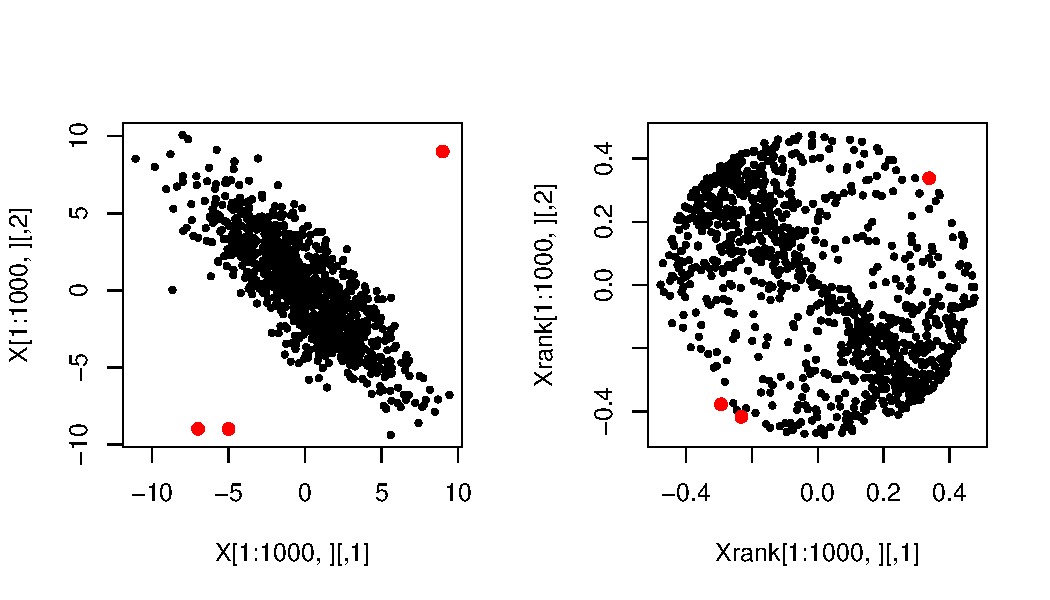
\includegraphics[height=6cm]{ranks.pdf}
	\caption{(Left) 1000 points randomly drawn from $\mathcal N_2\left((0,0)^T, \left(\protect\begin{smallmatrix} 5 & -4 \\ -4 & 5 \protect\end{smallmatrix}\right)\right) $ and (Right) their multivariate ranks based on halfspace depth}
	\label{fig:rankplot}
\end{figure}

Now consider the spectral decomposition for the covariance matrix of $F$: $\bfSigma = \bfGamma\bfLambda\bfGamma^T$, $\bfGamma$ being orthogonal and $\bfLambda$ diagonal with positive diagonal elements. Also normalize the original random variable as $\bfz = \bfGamma^T\bfLambda^{-1/2} (\bfx - \bfmu)$. In this setup, we can represent the transformed random variable as
%
\begin{eqnarray}
\tilde \bfx &=& \tilde D^- (\bfx, [\bfX]) \bfS(\bfx - \bfmu) \notag \\
&=& D^-  (\bfGamma\bfLambda^{1/2} \bfz + \bfmu, [\bfGamma\bfLambda^{1/2}\bfZ + \bfmu ]). \bfS(\bfGamma\bfLambda^{1/2} \bfz) \notag \\
&=& D^-  (\bfz, [\bfZ]) .\bfGamma \bfS(\bfLambda^{1/2}\bfz) \notag \\
&=& \left[ \bfGamma \bfLambda^{1/2} \frac{\| \bfz \|}{\|\bfLambda^{1/2} \bfz\|} \right]. D^-  (\bfz, [\bfZ]) \bfS(\bfz)
\label{equation:rankdecomp}
\end{eqnarray}
%
%Because of affine (thus rotational) invariance of a depth function, the depth (htped) value at $\bfz$ does not depend on the direction of $\bfz$, i.e. $\tilde D_{\bfZ}(\bfz)$ and $\bfS(\bfz)$ are independent. Furthermore,
%$$ Cov \left(\bfS (\bfz), \frac{\| \bfz \|}{\|\bfLambda^{1/2} \bfz\|} \right) = E \left(\bfS (\bfz). \frac{\| \bfz \|}{\|\bfLambda^{1/2} \bfz\|} \right) - E \bfS (\bfz) E \left(\frac{\| \bfz \|}{\|\bfLambda^{1/2} \bfz\|} \right) = E \left( \frac{\bfz}{\|\bfLambda^{1/2} \bfz\|} \right) = \bf0$$
%both $\bfS (\bfz)$ and $\bfz / \| \bfLambda^{1/2}\bfz \|$ are odd functions of $\bfz$, which has a circularly symmetric distribution, hence each of them has expectation $\bf0$. Consequently, we obtain an expression for the covariance matrix of $\tilde \bfX$:

following affine invariance of $D$ hence $D^-$. Now $D^- ( \bfz, [\bf Z])$ is an even function in $\bfz$ because of affine invariance, as is $\| \bfz \| / \|\bfLambda^{1/2} \bfz \|$. Since $\bfS(\bfz)$ is odd in $\bfz$ for spherically symmetric $\bfz$, it follows that $ \BE \tilde \bfX = {\bf 0}_p$. Consequently we obtain an expression for the covariance matrix of $\tilde \bfX$:

\begin{Theorem} \label{Theorem:covform}
Let the random variable $\bfX \in \mathbb{R}^p$ follow an elliptical distribution with center $\bfmu$ and covariance matrix $\bfSigma = \bfGamma\bfLambda\bfGamma^T$, its spectral decomposition. Then, given a depth function $D(.)$, the covariance matrix of the transformed random variable $\tilde\bfX$ is
%
\begin{align} \label{equation:covformEq1}
\BV(\tilde \bfX) = \bfGamma \tilde \bfLambda \bfGamma^T,\quad\mbox{with}\quad \tilde \bfLambda = \mathbb E_\bfZ \left[ (D^- ( \bfz, [\bfZ]) )^2 \frac{\bfLambda^{ 1/2 } \bfz \bfz^{T} \bfLambda^{ 1/2 }}{\bfz^T \bfLambda \bfz} \right]
\end{align}
%
where $\bfZ = (Z_1,...,Z_p)^T \sim \cN ({\bf 0}, \bfI_p)$, so that $\tilde \bfLambda$ is a diagonal matrix with diagonal entries
%
\begin{align}
\tilde \lambda_{i} = \BE_\bfZ \left[ \frac{(D^- ( \bfz, [\bfZ]) )^2 \lambda_i z_i^2}{\sum_{j=1}^p \lambda_j z_j^2} \right]
\end{align}
%
\end{Theorem}

We call $\tilde \bfSigma := \BV(\tilde \bfX)$ the Depth Covariance Matrix (DCM).  Notice that the matrix of eigenvectors of the covariance matrix of $\bfX$, i.e. $\bfGamma$, remains unchanged in the transformation $\bfX \mapsto \tilde \bfX$. As a result, the multivariate rank vectors can be used for robust principal component analysis, which we are going to discuss shortly. However, as one can see in the above expression, the diagonal entries of $\tilde \bfLambda$ do not change if a scale change is done on all entries of $\bfLambda$, meaning the $\tilde \bfLambda$ matrices corresponding to $F$ and $cF$ for some $c \neq 0$ will be same. Thus the DCM is not equivariant under affine transformations.

We need to follow the general framework of M-estimation with data-dependent weights in \cite{HuberBook81} to construct an affine equivariant counterpart of the DCM. Specifically, we implicitly define the Affine-equivariant Depth Covariance Matrix (ADCM) as
%
\begin{equation} \label{eqn:ADCM}
\tilde \bfSigma_\ot = \frac{1}{\BV(\tilde Z_1) } \BE \left[ \frac{(D^- (\bfx, [\bfX]))^2 (\bfx - \bfmu) (\bfx - \bfmu)^T}{(\bfx - \bfmu)^T \tilde \bfSigma_\ot ^{-1} (\bfx - \bfmu)} \right]
\end{equation}
%
Its affine equivariance follows from the fact that the weights $D^- (\bfx, [\bfX])$ depend only on the standardized quantities $\bfz$ that come from the underlying spherical distribution $G$. We solve \ref{eqn:ADCM} iteratively by obtaining a sequence of positive definite matrices $\tilde \bfSigma^{(k)}_\ot$ until convergence:
%
$$ \tilde \bfSigma^{(k+1)}_\ot = \frac{1}{\BV(\tilde Z_1) } \BE \left[ \frac{(D^- (\bfx, [\bfX]))^2 (\tilde \bfSigma^{(k)}_\ot)^{1/2} (\bfx - \bfmu) (\bfx - \bfmu)^T (\tilde \bfSigma^{(k)}_\ot)^{1/2}}{(\bfx - \bfmu)^T (\tilde \bfSigma^{(k)}_\ot)^{-1} (\bfx - \bfmu)} \right] $$
%

To ensure existence and uniqueness of this estimator, let us consider the class of scatter estimators $\bfSigma_M$ that are obtained as solutions of the following equation:
%
\begin{equation}
\BE_{ \bfZ_M } \left[ u( \| \bfz_M \| )  \frac{\bfz_M \bfz_M^T}{\| \bfz_M \|^2}  - v( \| \bfz_M \| ) \bfI_p \right] = 0
\end{equation}
%
with $\bfz_M = \bfSigma_M^{-1/2} (\bfx - \bfmu)$. The above equation produces a unique solution under the following assumptions on the scalar-valued functions $u$ and $v$ \citep{HuberBook81}:
%

\vspace{1em}
\noindent\textbf{(M1)} The function $u(r)/r^2$ is monotone decreasing, and $u(r)>0$ for $r>0$;

\noindent\textbf{(M2)}  The function $v(r)$ is monotone decreasing, and $v(r)>0$ for $r>0$;

\noindent\textbf{(M3)} Both $u(r)$ and $v(r)$ are bounded and continuous;

\noindent\textbf{(M4)} $u(0) / v(0) < p$;

\noindent\textbf{(M5)} For any hyperplane in the sample space $\mathcal X$, (i) $P(H) = \BE_\bfX \BI_{\bfx \in H} < 1 - p v(\infty) / u(\infty)$ and (ii) $P(H) \leq 1/p$.
%

\vspace{1em}
\noindent In our case we take $v(r) = \BV(\tilde Z_1)$, i.e. a constant, thus (M2) and (M3) are trivially satisfied. As for $u$, we notice that most well-known depth functions can be expressed as simple functions of the norm of the standardized random variable. For example, $PD (\bfz, [\bfZ]) = 1 - F_{01} (\| \bfz \|); MhD( \bfz, [\bfZ]) = (1+\| \bfz \|^2)^{-1}; HD (\bfz, [\bfZ]) = (1+\| \bfz \|/ MAD(F_{01}) )^{-1}$ etc., where $F_{01} \equiv \cE(0, 1, g)$, and MAD is median absolute deviation. Thus we can take $u$ as square of the corresponding inverse depth functions:
% \BV(Z1) breaks into two independent parts: depth and sign. So can check m4 and M5 here itself.
$$
u_{PD} (r) = F_{01}^2 (r); \quad u_{MhD}(r)  = \frac{r^4}{(1 + r^2)^2}; \quad u_{HSD}(r)  = \frac{r^2}{(1 + r/MAD(F_{01} ) )^2}
$$
%
%Here $G$ is the probability distribution function corresponding to the density generator $g$.

It is easy to verify that the above choices of $u$ satisfy (M1) and (M3). To check (M4) and (M5), first notice that $\bfZ$ has a spherically symmetric distribution, so that its norm and sign are independent. Since $D (\bfz, [\bfZ])$ depends only on $\| \bfz \|$, we have
%
$$
\BV(\tilde Z_1) = \BV \left( D^- (\bfZ, [\bfZ]) \frac{Z_1}{ \|\bfZ \|} \right) = \BV(D^-(\bfZ, [\bfZ])) \BV(S_1 (\bfZ)) = \frac{1}{p} \BV( D^- (\bfZ, [\bfZ]))
$$
%
as $\BV(\bfS(\bfZ)) = \BV((S_1(\bfZ), S_2(\bfZ), ..., S_p(\bfZ))^T) = \bfI_p/p$. Now for MhD and HD $u(\infty)=1, u(0)=0$, so (M4) and (M5) are immediate. To achieve this for PD, we only need to replace $u_{PD}(r)$ with $u_{PD}^*(r) = F_{01}^2(r) - 1/4$.

\subsection{Calculating the sample DCM and ADCM}
Let us denote $\BS (\bfx; \bfmu) = \bfS(\bfx - \bfmu) \bfS(\bfx - \bfmu)^T$. Then, given the depth function and known location center $\bfmu$, one can show that the vectorized form of $\sqrt n$-times the sample DCM, i.e. $(1/\sqrt n) \sum_{i=1}^n (D^- (\bfx_i, [\bfX]))^2 \BS(\bfx_i; \bfmu)$  has an asymptotic multivariate normal distribution with mean $\sqrt n. \ve ( \BE[ (D^- (\bfX, [\bfX]))^2 \BS(\bfX; \bfmu)])$ and a certain covariance matrix by straightforward application of the Central Limit Theorem (CLT). But in practice the population depth function $D (\bfx, [\bfX])$ is estimated by the depth function based on the empirical distribution function $[ \BX_n ]$, i.e. by $D (\bfx, [\BX_n])$ (recall from \ref{sec:scatter-sec2-location} that $\BX_n = (\bfX_1, \ldots \bfX_n)^T$). Here we make the following assumption regarding how $D^- (\bfx, [\bfX])$ is approximated by its sample counterpart:

\vspace{1em}
\noindent\textbf{(P5)} \textit{Uniform convergence}: $\sup_{\bfx \in \mathbb R^p} | D (\bfx, [\BX_n]) - D (\bfx, [\bfX]) | \raro 0$ as $n \raro \infty $.
\vspace{1em}

The assumption that empirical depths converge uniformly at all points $\bfx$ to their population versions holds under very mild conditions for several well known depth functions: for example projection depth \citep{zuo03} and simplicial depth \citep{Dumbgen92}. One also needs to replace the known location parameter $\bfmu$ by some estimator $\hat\bfmu_n$. Examples of robust estimators of location that are relevant here include the spatial median \citep{haldane48,brown83}, Oja median \citep{oja83}, projection median \citep{zuo03} etc. Now, given $D (., [\BX_n])$ and $\hat \bfmu_n$, to plug them into the sample DCM and still go through with the CLT we need the following result:

\begin{Lemma} \label{Lemma:lemma1}
Consider a random variable $\bfX \in \mathbb{R}^p$ having a continuous and symmetric distribution with location center $\bfmu$ such that $ \BE \|\bfx - \bfmu \|^{-3/2} < \infty$. Given $n$ random samples from this distribution, suppose $\hat\bfmu_n$ is an estimator of $\bfmu$ so that $\sqrt n (\hat\bfmu_n - \bfmu) = O_P(1) $. Then with the above notations, and given the assumption (D5) we have
%
$$ \sqrt n \left[
\frac{1}{n} \sum_{i=1}^n (D^- (\bfx_i, [\BX_n]))^2 \BS(\bfx_i; \hat\bfmu_n) -
\frac{1}{n} \sum_{i=1}^n (D^- (\bfx_i, [\bfX]))^2 \BS(\bfx_i; \bfmu) \right]
\stackrel{P}{\rightarrow} 0 $$
\end{Lemma}

Following this, we are now in a position to state the result for consistency of the sample DCM:

\begin{Theorem} \label{Theorem:rootn}
Consider $n$ iid samples from the distribution in Lemma \ref{Lemma:lemma1}. Then, given a depth function $D(., [\bfX])$ and an estimate of center $\hat\bfmu_n$ so that $\sqrt n(\hat \bfmu_n - \bfmu) = O_P(1)$,
%
\begin{eqnarray}
&& \hspace{-4em} \sqrt n \left[ \ve \left\{ \frac{1}{n} \sum_{i=1}^n (D^- (\bfx, [\BX_n]))^2 \BS(\bfx_i; \hat\bfmu_n) \right\} - \BE \left[ vec\left\{ (D^- (\bfx, [\bfX]))^2 \BS(\bfx; \bfmu) \right\} \right] \right] \\\notag
&& \leadsto \cN_{p^2} ({\bf 0}, \tilde \bfV (F))
\end{eqnarray}
%
with $\tilde \bfV (F) = \BV \left[ \ve \left\{ (D^- (\bfx_i, [\bfX]))^2 \BS(\bfx; \bfmu) \right\} \right]$.
\end{Theorem}

\noindent This holds for any general non-degenerate $F$. In case $F$ is elliptical, an elaborate form of the covariance matrix $\tilde \bfV_F$ explicitly specifying each of its elements (more directly those of its $\bfGamma^T$-rotated version) can be obtained, which is given in \ref{subsec:appA}. This form is useful when deriving limiting distributions of eigenvectors and eigenvalues of the sample DCM.

In contrast to the DCM, the issue of estimating $\bfmu$ to plug into the ADCM is easily handled by simultaneously solving for the location and scatter functionals ($\bfmu_\ot, \tilde \bfSigma_\ot$):
%
\begin{eqnarray}
\BE \left[ \frac{\tilde \bfSigma_\ot^{-1/2} (\bfx - \bfmu_\ot)}{ \| \tilde \bfSigma_\ot^{-1/2}(\bfx - \bfmu_\ot) \|} \right] &=& {\bf 0}_p \label{eqn:AffineMedian}\\
\BE \left[ \frac{( D^- (\bfx, [\bfX] ) )^2 \tilde \bfSigma_\ot^{-1/2} (\bfx - \bfmu_\ot) (\bfx - \bfmu_\ot)^T \tilde \bfSigma_\ot^{-1/2}}{(\bfx - \bfmu_\ot)^T \tilde \bfSigma_\ot^{-1} (\bfx - \bfmu_\ot)} \right] &=& \BV(\tilde Z_1) \bfI_p \label{eqn:AffineCov}
\end{eqnarray}
%
In the general framework of \ref{eqn:ADCM}, for any fixed $\bfSigma_M$ there exists a unique and fixed solution of the location problem $\BE_{\bfZ_M} (w(\| \bfz_M \| \bfz_M) = {\bf 0}_p $ under the following condition:

\vspace{1em}
\noindent\textbf{(M6)} The function $w(r)r$ is monotone increasing for $r>0$.

\vspace{1em}
\noindent This condition is easy to verify for our choice of the weights: $w(\| \bfz_M \| ) = \tilde D (\bfz_M, [\bfZ_M]) / \| \bfz_M \|$. Consequently, uniqueness of any simultaneous fixed point solution of \ref{eqn:AffineMedian} and \ref{eqn:AffineCov} is guaranteed when $\bfX$ has a symmetric distribution \citep{HuberBook81}.

In practice it is difficult to calculate the scale multiple $\BV(\tilde Z_1)$ analytically for known depth functions and an arbitrary $F$. Hence we instead calculate the standardized version if the ADCM: $\tilde \bfSigma_\ot^* = \tilde \bfSigma_\ot / \BV(\tilde Z_1)$ (so that the determinant equals 1), alongwith $\bfmu_\ot$ using the following iterative algorithm:

\begin{enumerate}
\item Start from some initial estimates $(\bfmu_\ot^{(0)}, \tilde \bfSigma^{(0)}_\ot)$. Set $t=0$;

\item Calculate the standardized observations $\bfz_i^{(t)} = (\tilde \bfSigma^{(t)}_\ot)^{-1/2} (\bfx_i - \bfmu_\ot^{(t)})$;

\item Update the location estimate:
%
$$
\bfmu_\ot^{(t+1)} = \frac{\sum_{i=1}^n \tilde \bfx_i / \| \bfz_i^{(t)} \| }{\sum_{i=1}^n 1 / \| \bfz_i^{(t)} \|}
$$
%
\item Update the scatter estimate:
%
\begin{eqnarray*}
\tilde \bfSigma_\ot^{*(t+1)} &=& \frac{1}{n} \sum_{i=1}^n \frac{( D^- (\bfx_i, [\BX_n]))^2 (\bfx_i - \bfmu_\ot^{(t+1)})(\bfx_i - \bfmu_\ot^{(t+1)})^T}{\| \bfz_i^{(t)} \|^2}\\
\tilde \bfSigma_\ot^{*(t+1)} & \leftarrow & \frac{\tilde \bfSigma_\ot^{*(t+1)}}{\text{det} (\tilde \bfSigma_\ot^{*(t+1)})^{1/p}}
\end{eqnarray*}
%
\item Continue until convergence.
\end{enumerate}
%
Notice that owing to the uniform convergence property we can safely replace $D^-(\bfx_i, [\bfX])$ with its sample version and use the iterative algorithm above to obtain a consistent estimate of the of the solution of \ref{eqn:AffineCov}.

\subsection{Robust PCA using eigenvectors of DCM}

We shall now elaborate on using the DCM for robust principal components analysis. From now on we assume that the eigenvalues of $\bfSigma$ are distinct: $\lambda_1 > \lambda_2 > ... > \lambda_p$ to obtain asymptotic distributions of its eigenvectors. In case any of the eigenvalues have multiplicity larger than 1, limiting distributions of the corresponding eigenprojection matrices can be obtained analogous to those of the sign covariance matrix \citep{magyar14}.

\subsubsection{Influence functions}
We start by deriving the influence functions for eigenvectors of the DCM and ADCM. This will help in demonstrating the robustness of their estimates, as well as deriving their asymptotic efficiencies. Influence functions of the DCM as well as its eigenvectors and eigenvalues, which are essential to understand how much influence a sample point, especially an infinitesimal contamination, has on any functional on the distribution \citep{HampelBook86}. Given any probability distribution $F$, the influence function of any point $\bfx_0$ in the sample space $\mathcal{X}$ for some functional $T(F)$ on the distribution is defined as
%
$$ IF(\bfx_0; T,F) = \lim_{\epsilon \rightarrow 0} \frac{1}{\epsilon} (T(F_\epsilon) - T(F)) $$
%
where $F_\epsilon$ is $F$ with an additional mass of $\epsilon$ at $\bfx_0$, i.e. $F_\epsilon = (1-\epsilon)F + \epsilon \delta_{\bfx_0}$; $\delta_{\bfx_0}$ being the distribution with point mass at $\bfx_0$. When $T(F) = \BE_F g$ for some $F$-integrable function $g$, $IF(\bfx_0; T,F) = g(\bfx_0) - T(F)$. It now follows that for the DCM,
%
$$ IF(\bfx_0; \tilde \bfSigma, F) = ( D^- ( \bfx_0, [\bfX]))^2 \BS(\bfx_0; \bfmu) - \tilde \bfSigma $$

Following \cite{croux00}, we now get the influence function of the $i^\text{th}$ eigenvector of $\tilde \bfSigma$, say $\tilde \bfGamma = (\tilde\bfgamma_{1}, \ldots, \tilde \bfgamma_{p}); i = 1,...,p$:
%
\begin{eqnarray}
IF(\bfx_0; \tilde\bfgamma_{i}, F) &=& \sum_{k=1; k \neq i}^p \frac{1}{\tilde\lambda_{i} - \tilde\lambda_{k}} \left\{ \bfgamma^T_k IF(\bfx_0; \tilde \bfSigma, \bfgamma_i) \right\} \bfgamma_k \notag \\
&=& \sum_{k=1; k \neq i}^p \frac{1}{\tilde \lambda_{i} - \tilde \lambda_{k}} \left\{ \bfgamma^T_k ( D^-(\bfx_0, [\bfX]))^2 \BS(\bfx_0; \bfmu) \bfgamma_i - \lambda_{i} \bfgamma_k^T \bfgamma_i \right\} \bfgamma_k \notag \\
&=& \sum_{k=1; k \neq i}^p \frac{\sqrt{\lambda_i \lambda_k} z_{0i} z_{0k}}{ \lambda_{i} - \lambda_{k}}. \frac{ ( D^- (\bfz_0, [\bfZ]))^2 }{ \bfz_0^T \bfLambda \bfz_0} \bfgamma_k
\end{eqnarray}
%
where $\bfGamma^T \bfLambda^{-1/2} (\bfx_0 - \bfmu) = \bfz_0 = (z_{01},...,z_{0p})^T$. Clearly this influence function will be bounded, which indicates good robustness properties of principal components.

For the ADCM, we first notice that the influence function of any affine equivariant estimate of scatter $\bfC$ can be expressed as
%
$$
IF(\bfx_0, \bfC, F) = \alpha_\bfC (\| \bfz_0 \| ) \frac{\bfz_0 \bfz_0^T}{ \bfz_0^T \bfz_0} - \beta_\bfC( \| \bfz_0 \| ) \bfC
$$
%
for scalar valued functions $\alpha_\bfC, \beta_\bfC$ \citep{HampelBook86}. Following this, the influence function of an eigenvector $\bfgamma_{\bfC,i}$ of $\bfC$ is derived:
%
$$
IF(\bfx_0, \bfgamma_{\bfC,i}, F) = \alpha_\bfC(\| \bfz_0 \|) \sum_{k=1, k \neq i}^p \frac{\sqrt {\lambda_i \lambda_k}}{\lambda_i - \lambda_k}. \frac{z_{0i} z_{0k}}{\bfz_0^T \bfz_0} \bfgamma_k
$$
%
When $\bfC=\bfSigma_M$, i.e. the solution to \ref{eqn:ADCM}, then \cite{HuberBook81} shows that
%
$$
\alpha_\bfC (\| \bfz_0 \|) = \frac{p(p+2) u (\| \bfz_0 \|)}{ \BE_G \left[ p u(\| \bfy \| ) + u'(\| \bfy \|) \| \bfy \| \right] }
$$
%
Setting $u( \| \bfz_0 \|) = ( D^- (\bfz_0, [\bfZ]))^2$ ensures that the influence function of eigenvectors of the ADCM is bounded as well as increasing in magnitude with $\| \bfz_0 \|$.

\begin{figure}
	\centering
		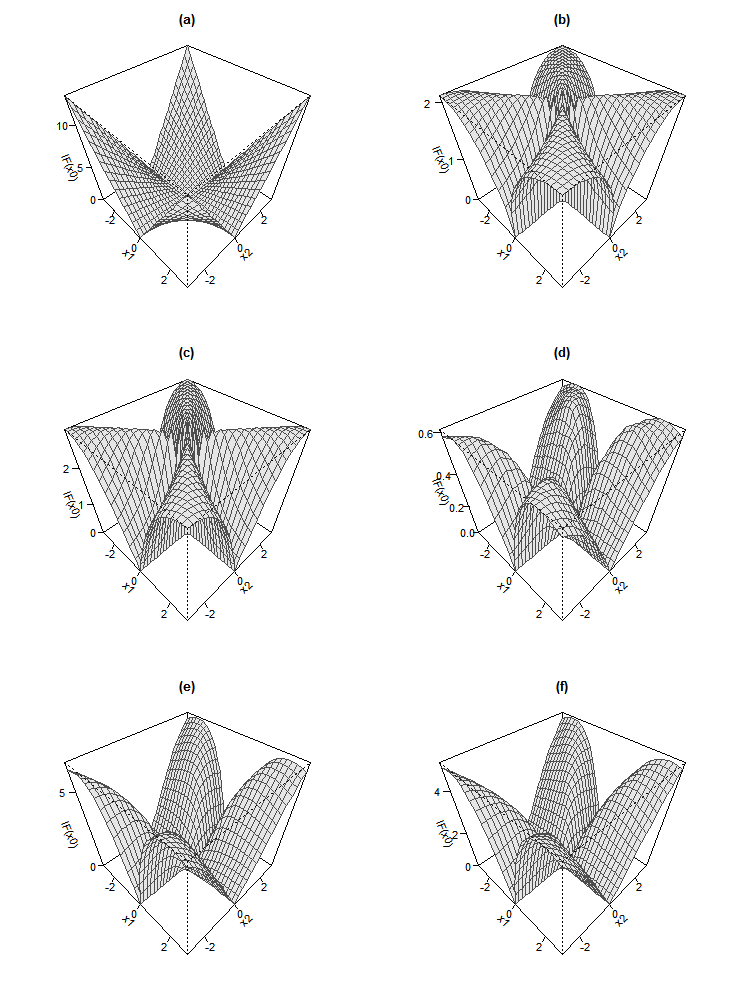
\includegraphics[width=12cm]{IFnorm.png}
	\caption{Plot of the norm of influence function for first eigenvector of (a) sample covariance matrix, (b) SCM, (c) Tyler's scatter matrix and DCMs for (d) Halfspace depth, (e) Mahalanobis depth, (f) Projection depth for a bivariate normal distribution with $\bfmu = {\bf 0}, \bfSigma = \diag(2,1)$}
	\label{fig:IFnorm}
\end{figure}

In \ref{fig:IFnorm} we consider first eigenvectors of our scatter estimates, as well as two well-known robust estimates of scatter: the Sign Covariance Matrix (SCM) \citep{taskinen12} and Tyler's shape matrix \citep{tyler87}, for the $\mathcal{N}_2((0,0)^T, \diag(2,1))$ and plot norms of these influence functions for different values of $\bfx_0$. Influence function for the $i^\text{th}$ eigenvectors of these two matrices (say $\bfgamma_{S,i}$ and $\bfgamma_{T,i}$, respectively) are as follows:
%
\begin{eqnarray*}
\quad IF(\bfx_0; \bfgamma_{S,i}, F) &=& \sum_{k=1; k \neq i}^p \frac{\sqrt{\lambda_i \lambda_k}}{\lambda_{S,i} - \lambda_{S,k}}. \frac{z_{0i} z_{0k}}{\bfz_0^T \bfLambda \bfz_0} \bfgamma_k, \text{ with } \lambda_{S,i} = \BE_\bfZ \left( \frac{\lambda_i z_i^2}{\sum_{j=1}^p \lambda_j z_j^2} \right) \\
IF(\bfx_0; \bfgamma_{T,i}, F) &=& (p+2) \sum_{k=1; k \neq i}^p \frac{\sqrt{\lambda_i \lambda_k}}{\lambda_i - \lambda_k}. \frac{z_{0i} z_{0k}}{\bfz_0^T \bfz_0} \bfgamma_k 
\end{eqnarray*}
%
Their corresponding plots demonstrate the `inlier effect', i.e. points close to symmetry center and the center itself having high influence, which results in loss of efficiency. The influence function for the sample covariance matrix is obtained by replacing $(p+2)$ by $\| \bfz_0 \|^2$ in the expression of $IF(\bfx_0; \bfgamma_{T,i}, F)$ above, hence is unbounded and the corresponding eigenvector estimators are not robust. In comparison, all three DCMs considered here have a bounded influence function as well as small values of the influence function at `deep' points.

\subsubsection{Asymptotic and finite-sample efficiencies}

%Unlike affine equivariant estimators of shape, the Asymptotic Relative Efficiency (ARE) of eigenvectors (with respect to any other affine equivariant estimator) can not be simplified as a ratio of two scalar quantities dependent on only the distribution of $\| \bfz \|$ (e.g. \cite{taskinen12,ollilia03}).
Suppose $\hat \bfV$ is a $\sqrt n$-consistent estimator of a scatter functional $\bfV$. Then the asymptotic variance of its eigenvectors are \citep{anderson}
%
\begin{equation} \label{equation:covevEq}
A\BV(\sqrt n\hat \bfgamma_{v,i}) = \sum_{k=1; k \neq i}^p \frac{\lambda_{v,i} \lambda_{v,k}}{(\lambda_{v,i} - \lambda_{v,k})^2} \bfgamma_{v,k} \bfgamma_{v,k}^T
\end{equation}
%
On the other hand, asymptotic variances of eigenvectors of the DCM can be derived using an approach similar to \cite{taskinen12}:
%
\begin{equation} \label{equation:dcmevEq}
A\BV( \sqrt n\hat \tilde \bfgamma_{i} ) = \sum_{k=1; k \neq i}^p \frac{1}{(\tilde \lambda_k - \tilde \lambda_i)^2} \BE \left[ \frac{(D^- (\bfz, [\bfZ]))^4 \lambda_i \lambda_k z_i^2 z_k^2}{(\bfz^T \Lambda \bfz)^2} \right] \bfgamma_k \bfgamma_k^T
\end{equation}
%
We discuss this in detail in \ref{subsection:appB}. Following the above, we can now derive the asymptotic relative efficiencies of eigenvectors from the sample DCM with respect to the sample covariance matrix:
%
\begin{eqnarray*}
ARE(\hat{ \tilde\bfgamma}_i, \hat\bfgamma_i; F) &=& \frac{\Tr( A\BV(\sqrt n\hat \bfgamma_i))}{\Tr( A\BV(\sqrt n \hat{ \tilde\bfgamma}_i )) }\\
&=& \left[\sum_{k=1; k \neq i}^p \frac{\lambda_i \lambda_k }{ (\lambda_i - \lambda_k )^2 } \right] \left[ \sum_{k=1; k \neq i}^p \frac{ \lambda_i \lambda_k }{ ( \tilde\lambda_{i} - \tilde\lambda_{k})^2} \BE \left( \frac{ ( D^- (\bfz, [\bfZ]) )^4 z_i^2 z_k^2}{(\bfz^T \bfLambda \bfz)^2} \right) \right]^{-1}
\end{eqnarray*}

Obtaining ARE of the ADCM is, in comparison to DCM, more straightforward. The asymptotic covariance matrix of an eigenvector of the affine equivariant scatter functional $\bfC$ is given by:
%
$$
A\BV(\sqrt n  \hat\bfgamma_{\bfC,j}) = A\BV(c_{12}, F_0) \sum_{k=1, k \neq i}^p \frac{\lambda_i \lambda_k}{\lambda_i - \lambda_k}. \bfgamma_i \bfgamma_k^T
$$
%
where $A\BV(c_{12}, F_0)$ is the asymptotic variance of an off-diagonal element of $\bfC$ when the underlying distribution is $F_0 \equiv \cE ({\bf 0}_p, \bfI_p, g)$. Following \cite{croux00} this equals
%
$$
A\BV(\bfc_{12}, F_0) = \BE_{F_0} \left[ \alpha_\bfC (\| \bfz \|)^2 (S_1(\bfz)S_2 (\bfz))^2 \right] = \BE_{F_0} \alpha_\bfC (\| \bfz \|)^2 . \BE_{F_0} (S_1(\bfz)S_2 (\bfz))^2 
$$
% 
again using the fact that $\|\bfZ\|$ and $\bfS(\bfZ)$ are independent when $\bfZ \sim F_0$. It now follows that
%
\begin{equation}
ARE (\hat\bfgamma_{\bfC,i}, \hat\bfgamma_{ \bfSigma,i}; F) = \frac{\BE_{F_0} \alpha_{\bfSigma} (\| \bfz \|)^2}{\BE_{F_0} \alpha_\bfC (\| \bfz \|)^2} = \frac{\BE_{F_0} \| \bfz \|^4. \left[ \BE_{F_0} ( p u \| \bfz\| + u'( \| \bfz \|) \| \bfz \| ) \right]^2}{\BE_{F_0} (u(\| \bfz \|))^2}
\end{equation}
%

\ref{table:AREtable} considers 6 different elliptic distributions (namely, bivariate $t$ with df = 5, 6, 10, 15, 25 and bivariate normal) and summarizes ARE for first eigenvectors for ADCMs corresponding to projection depth (PD-ACM) and halfspace depth (HD-ACM). Due to difficulty of analytically obtain the AREs, we calculate them using Monte-Carlo simulation of $10^6$ samples and subsequent numerical integration. The ADCM seems to be particularly efficient in lower dimensions for distributions with heavier tails ($t_5$ and $t_6$), while for distributions with lighter tails, the AREs increase with data dimension. At higher values of $p$ the ADCM is almost as efficient as the sample covarnace matrix when the data comes from multivariate normal distribution.

\begin{table}[t]
\begin{footnotesize}
\centering
    \begin{tabular}{c|cccc|cccc}
    \hline
    & \multicolumn{4}{c|}{PD-ACM} & \multicolumn{4}{c}{HD-ACM} \\\cline{2-9}
    Distribution & $p=2$  & $p=5$  & $p=10$ & $p=20$ & $p=2$  & $p=5$  & $p=10$ & $p=20$ \\ \hline
    $t_5$           & 4.73 & 3.99 & 3.46 & 3.26 & 4.18 & 3.63 & 3.36 & 3.15 \\
    $t_6$           & 2.97 & 3.28 & 2.49 & 2.36 & 2.59 & 2.45 & 2.37 & 2.32 \\
    $t_{10}$          & 1.45 & 1.47 & 1.49 & 1.52 & 1.30 & 1.37 & 1.43 & 1.49 \\
    $t_{15}$          & 1.15 & 1.19 & 1.23 & 1.27 & 1.01 & 1.10 & 1.17 & 1.24 \\
    $t_{25}$          & 0.97 & 1.02 & 1.07 & 1.11 & 0.85 & 0.94 & 1.02 & 1.08 \\
    MVN          & 0.77 & 0.84 & 0.89 & 0.93 & 0.68 & 0.77 & 0.84 & 0.91 \\ \hline
    \end{tabular}
    \caption{Table of AREs of the ADCM for different choices of $p$ and data-generating distributions, and two choices of depth functions}
    \label{table:AREtable}
\end{footnotesize}
\end{table}

\begin{table}[ht]
\centering
\begin{footnotesize}
    \begin{tabular}{c|cc|ccc|ccc}
    \hline
    $t_5, p=2$    & SCM  & Tyler & HDCM & MHDCM & PDCM & HD-wCM & MhD-wCM & PD-wCM \\ \hline
    $n$=20                   & 0.80 & 0.83  & 0.95   & 0.95   & 0.89  & 1.00    & 0.96    & 0.89   \\
    $n$=50                   & 0.86 & 0.90  & 1.25   & 1.10   & 1.21  & 1.32    & 1.13    & 1.25   \\
    $n$=100                  & 1.02 & 1.04  & 1.58   & 1.20   & 1.54  & 1.67    & 1.24    & 1.63   \\
    $n$=300                  & 1.24 & 1.28  & 1.81   & 1.36   & 1.82  & 1.93    & 1.44    & 1.95   \\
    $n$=500                  & 1.25 & 1.29  & 1.80   & 1.33   & 1.84  & 1.91    & 1.39    & 1.97   \\ \hline
    $t_6, p=2$    & SCM  & Tyler & HDCM & MHDCM & PDCM & HD-wCM & MhD-wCM & PD-wCM \\ \hline
    $n$=20                   & 0.77 & 0.79  & 0.92   & 0.92   & 0.86  & 0.96    & 0.92    & 0.85   \\
    $n$=50                   & 0.76 & 0.78  & 1.11   & 1.00   & 1.08  & 1.17    & 1.03    & 1.13   \\
    $n$=100                  & 0.78 & 0.79  & 1.27   & 1.06   & 1.33  & 1.35    & 1.11    & 1.41   \\
    $n$=300                  & 0.88 & 0.91  & 1.29   & 1.09   & 1.35  & 1.38    & 1.15    & 1.45   \\
    $n$=500                  & 0.93 & 0.96  & 1.37   & 1.13   & 1.40  & 1.44    & 1.19    & 1.48   \\ \hline
    $t_{10}, p=2$ & SCM  & Tyler & HDCM & MHDCM & PDCM & HD-wCM & MhD-wCM & PD-wCM \\ \hline
    $n$=20                   & 0.70 & 0.72  & 0.83   & 0.84   & 0.77  & 0.89    & 0.87    & 0.79   \\
    $n$=50                   & 0.58 & 0.60  & 0.90   & 0.84   & 0.86  & 0.95    & 0.88    & 0.91   \\
    $n$=100                  & 0.57 & 0.59  & 0.92   & 0.87   & 0.97  & 0.98    & 0.90    & 1.03   \\
    $n$=300                  & 0.62 & 0.64  & 0.93   & 0.85   & 0.99  & 0.99    & 0.91    & 1.06   \\
    $n$=500                  & 0.62 & 0.65  & 0.93   & 0.86   & 1.00  & 1.00    & 0.92    & 1.08   \\ \hline
    $t_{15}, p=2$ & SCM  & Tyler & HDCM & MHDCM & PDCM & HD-wCM & MhD-wCM & PD-wCM \\ \hline
    $n$=20                   & 0.63 & 0.66  & 0.76   & 0.78   & 0.72  & 0.81    & 0.81    & 0.73   \\
    $n$=50                   & 0.52 & 0.52  & 0.79   & 0.75   & 0.80  & 0.84    & 0.79    & 0.85   \\
    $n$=100                  & 0.51 & 0.52  & 0.83   & 0.77   & 0.88  & 0.88    & 0.81    & 0.94   \\
    $n$=300                  & 0.55 & 0.56  & 0.84   & 0.79   & 0.91  & 0.89    & 0.84    & 0.98   \\
    $n$=500                  & 0.56 & 0.59  & 0.85   & 0.80   & 0.93  & 0.91    & 0.86    & 0.99   \\ \hline
    $t_{25}, p=2$ & SCM  & Tyler & HDCM & MHDCM & PDCM & HD-wCM & MhD-wCM & PD-wCM \\ \hline
    $n$=20                   & 0.63 & 0.65  & 0.77   & 0.79   & 0.74  & 0.80    & 0.81    & 0.74   \\
    $n$=50                   & 0.49 & 0.50  & 0.73   & 0.71   & 0.76  & 0.78    & 0.75    & 0.80   \\
    $n$=100                  & 0.45 & 0.46  & 0.73   & 0.69   & 0.81  & 0.78    & 0.73    & 0.87   \\
    $n$=300                  & 0.51 & 0.52  & 0.78   & 0.75   & 0.87  & 0.83    & 0.79    & 0.94   \\
    $n$=500                  & 0.53 & 0.55  & 0.79   & 0.75   & 0.87  & 0.84    & 0.80    & 0.94   \\ \hline
    $\cN_p$, $p=2$                & SCM  & Tyler & HDCM & MHDCM & PDCM & HD-wCM & MhD-wCM & PD-wCM \\ \hline
    $n$=20                   & 0.56 & 0.60  & 0.69   & 0.71   & 0.67  & 0.73    & 0.74    & 0.68   \\
    $n$=50                   & 0.42 & 0.43  & 0.66   & 0.66   & 0.70  & 0.71    & 0.69    & 0.75   \\
    $n$=100                  & 0.42 & 0.43  & 0.69   & 0.66   & 0.77  & 0.74    & 0.71    & 0.83   \\
    $n$=300                  & 0.47 & 0.49  & 0.71   & 0.69   & 0.82  & 0.76    & 0.73    & 0.88   \\
    $n$=500                  & 0.48 & 0.50  & 0.73   & 0.71   & 0.83  & 0.78    & 0.76    & 0.89   \\ \hline
    \end{tabular}
\caption{Finite sample efficiencies of several scatter matrices: $p=2$, $t_v$ is $t$-distribution with $v$ degrees of freedom, $\cN_p$ is $p$-variate normal}
\label{table:FSEtable2}
\end{footnotesize}
\end{table}
%
\begin{table}[ht]
\begin{footnotesize}
   \begin{tabular}{c|cc|ccc|ccc}
    \hline
    $t_5, p=3$    & SCM  & Tyler & HDCM & MHDCM & PDCM & HD-wCM & MhD-wCM & PD-wCM \\ \hline
    $n$=20             & 0.96 & 0.97  & 1.06   & 1.03   & 0.99  & 1.07    & 1.06    & 0.97   \\
    $n$=50             & 1.07 & 1.08  & 1.28   & 1.20   & 1.18  & 1.33    & 1.23    & 1.20   \\
    $n$=100            & 1.12 & 1.15  & 1.49   & 1.31   & 1.40  & 1.57    & 1.38    & 1.48   \\
    $n$=300            & 1.49 & 1.54  & 2.09   & 1.82   & 2.07  & 2.19    & 1.93    & 2.18   \\
    $n$=500            & 1.60 & 1.66  & 2.18   & 1.87   & 2.21  & 2.27    & 1.95    & 2.30   \\ \hline
    $t_6, p=3$    & SCM  & Tyler & HDCM & MHDCM & PDCM & HD-wCM & MhD-wCM & PD-wCM \\ \hline
    $n$=20             & 0.90 & 0.92  & 1.00   & 0.99   & 0.95  & 1.02    & 1.01    & 0.94   \\
    $n$=50             & 0.95 & 0.96  & 1.16   & 1.09   & 1.09  & 1.21    & 1.14    & 1.11   \\
    $n$=100            & 0.98 & 0.99  & 1.32   & 1.22   & 1.25  & 1.38    & 1.27    & 1.29   \\
    $n$=300            & 1.10 & 1.14  & 1.57   & 1.40   & 1.58  & 1.62    & 1.47    & 1.64   \\
    $n$=500            & 1.17 & 1.20  & 1.57   & 1.43   & 1.60  & 1.63    & 1.51    & 1.67   \\ \hline
    $t_{10}, p=3$ & SCM  & Tyler & HDCM & MHDCM & PDCM & HD-wCM & MhD-wCM & PD-wCM \\ \hline
    $n$=20             & 0.87 & 0.88  & 0.95   & 0.94   & 0.90  & 0.97    & 0.98    & 0.89   \\
    $n$=50             & 0.77 & 0.79  & 0.96   & 0.92   & 0.94  & 0.99    & 0.96    & 0.95   \\
    $n$=100            & 0.75 & 0.76  & 1.02   & 0.95   & 1.01  & 1.06    & 1.00    & 1.05   \\
    $n$=300            & 0.73 & 0.75  & 1.03   & 0.98   & 1.10  & 1.08    & 1.03    & 1.15   \\
    $n$=500            & 0.73 & 0.76  & 1.02   & 0.98   & 1.09  & 1.06    & 1.02    & 1.14   \\ \hline
    $t_{15}, p=3$ & SCM  & Tyler & HDCM & MHDCM & PDCM & HD-wCM & MhD-wCM & PD-wCM \\ \hline
    $n$=20             & 0.84 & 0.86  & 0.92   & 0.92   & 0.89  & 0.94    & 0.94    & 0.87   \\
    $n$=50             & 0.75 & 0.76  & 0.92   & 0.90   & 0.90  & 0.96    & 0.94    & 0.93   \\
    $n$=100            & 0.66 & 0.67  & 0.91   & 0.87   & 0.95  & 0.96    & 0.92    & 1.00   \\
    $n$=300            & 0.61 & 0.64  & 0.90   & 0.87   & 1.00  & 0.93    & 0.91    & 1.04   \\
    $n$=500            & 0.65 & 0.67  & 0.89   & 0.87   & 0.99  & 0.93    & 0.91    & 1.03   \\ \hline
    $t_{25}, p=3$ & SCM  & Tyler & HDCM & MHDCM & PDCM & HD-wCM & MhD-wCM & PD-wCM \\ \hline
    $n$=20             & 0.78 & 0.79  & 0.87   & 0.89   & 0.87  & 0.89    & 0.92    & 0.86   \\
    $n$=50             & 0.70 & 0.71  & 0.88   & 0.86   & 0.88  & 0.91    & 0.90    & 0.90   \\
    $n$=100            & 0.61 & 0.63  & 0.86   & 0.83   & 0.89  & 0.90    & 0.88    & 0.94   \\
    $n$=300            & 0.58 & 0.59  & 0.83   & 0.80   & 0.92  & 0.87    & 0.85    & 0.98   \\
    $n$=500            & 0.62 & 0.64  & 0.83   & 0.82   & 0.94  & 0.88    & 0.87    & 0.99   \\ \hline
    $\cN_p$, $p=3$   & SCM  & Tyler & HDCM & MHDCM & PDCM & HD-wCM & MhD-wCM & PD-wCM \\ \hline
    $n$=20             & 0.76 & 0.78  & 0.85   & 0.87   & 0.84  & 0.87    & 0.90    & 0.83   \\
    $n$=50             & 0.66 & 0.67  & 0.82   & 0.81   & 0.84  & 0.86    & 0.86    & 0.86   \\
    $n$=100            & 0.56 & 0.58  & 0.77   & 0.75   & 0.83  & 0.82    & 0.79    & 0.87   \\
    $n$=300            & 0.53 & 0.55  & 0.75   & 0.74   & 0.85  & 0.79    & 0.78    & 0.90   \\
    $n$=500            & 0.56 & 0.58  & 0.76   & 0.76   & 0.87  & 0.80    & 0.80    & 0.92   \\ \hline
    \end{tabular}
\caption{Finite sample efficiencies of several scatter matrices: $p=2$, $t_v$ is $t$-distribution with $v$ degrees of freedom, $\cN_p$ is $p$-variate normal}
\label{table:FSEtable3}
\end{footnotesize}
\end{table}
%
\begin{table}[ht]
\begin{footnotesize}
    \begin{tabular}{c|cc|ccc|ccc}
    \hline
    $t_5, p=4$    & SCM  & Tyler & HDCM & MHDCM & PDCM & HD-wCM & MhD-wCM & PD-wCM \\ \hline
    $n$=20             & 1.04 & 1.02  & 1.10   & 1.07   & 1.02  & 1.09    & 1.07    & 0.98   \\
    $n$=50             & 1.08 & 1.08  & 1.16   & 1.16   & 1.13  & 1.19    & 1.19    & 1.13   \\
    $n$=100            & 1.31 & 1.31  & 1.42   & 1.38   & 1.36  & 1.46    & 1.44    & 1.36   \\
    $n$=300            & 1.46 & 1.54  & 1.81   & 1.76   & 1.95  & 1.88    & 1.88    & 1.95   \\
    $n$=500            & 1.92 & 1.93  & 2.23   & 2.03   & 2.31  & 2.35    & 2.19    & 2.39   \\ \hline
    $t_6, p=4$    & SCM  & Tyler & HDCM & MHDCM & PDCM & HD-wCM & MhD-wCM & PD-wCM \\ \hline
    $n$=20             & 1.00 & 1.05  & 1.03   & 1.05   & 1.00  & 1.04    & 1.04    & 0.95   \\
    $n$=50             & 1.03 & 1.01  & 1.13   & 1.12   & 1.11  & 1.19    & 1.17    & 1.10   \\
    $n$=100            & 1.08 & 1.12  & 1.25   & 1.23   & 1.27  & 1.24    & 1.25    & 1.22   \\
    $n$=300            & 1.34 & 1.36  & 1.64   & 1.52   & 1.60  & 1.67    & 1.61    & 1.68   \\
    $n$=500            & 1.26 & 1.34  & 1.55   & 1.49   & 1.60  & 1.65    & 1.61    & 1.69   \\ \hline
    $t_{10}, p=4$ & SCM  & Tyler & HDCM & MHDCM & PDCM & HD-wCM & MhD-wCM & PD-wCM \\ \hline
    $n$=20             & 0.90 & 0.89  & 0.95   & 0.98   & 0.98  & 0.96    & 1.01    & 0.95   \\
    $n$=50             & 0.90 & 0.91  & 1.01   & 0.98   & 0.98  & 1.03    & 1.04    & 0.99   \\
    $n$=100            & 0.87 & 0.87  & 0.93   & 0.95   & 1.01  & 0.99    & 1.01    & 1.05   \\
    $n$=300            & 0.87 & 0.87  & 1.09   & 1.09   & 1.17  & 1.14    & 1.16    & 1.23   \\
    $n$=500            & 0.88 & 0.92  & 1.10   & 1.10   & 1.23  & 1.19    & 1.22    & 1.29   \\ \hline
    $t_{15}, p=4$ & SCM  & Tyler & HDCM & MhDCM & PDCM & HD-wCM & MhD-wCM & PD-wCM \\ \hline
    $n$=20             & 0.92 & 0.90  & 0.94   & 0.94   & 0.96  & 0.95    & 0.97    & 0.89   \\
    $n$=50             & 0.82 & 0.83  & 0.88   & 0.91   & 0.93  & 0.88    & 0.93    & 0.93   \\
    $n$=100            & 0.84 & 0.87  & 0.92   & 0.95   & 1.00  & 0.93    & 0.96    & 1.00   \\
    $n$=300            & 0.73 & 0.75  & 0.96   & 0.99   & 1.10  & 1.00    & 1.06    & 1.12   \\
    $n$=500            & 0.73 & 0.76  & 0.95   & 0.96   & 1.06  & 0.94    & 0.97    & 1.06   \\ \hline
    $t_{25}, p=4$ & SCM  & Tyler & HDCM & MhDCM & PDCM & HD-wCM & MhD-wCM & PD-wCM \\ \hline
    $n$=20             & 0.89 & 0.92  & 0.92   & 0.92   & 0.90  & 0.96    & 0.95    & 0.89   \\
    $n$=50             & 0.82 & 0.84  & 0.89   & 0.90   & 0.91  & 0.93    & 0.96    & 0.92   \\
    $n$=100            & 0.77 & 0.76  & 0.90   & 0.90   & 0.96  & 0.94    & 0.98    & 1.04   \\
    $n$=300            & 0.73 & 0.77  & 0.93   & 0.91   & 0.98  & 1.00    & 0.98    & 1.03   \\
    $n$=500            & 0.67 & 0.71  & 0.83   & 0.83   & 0.96  & 0.88    & 0.90    & 1.00   \\ \hline
    $\cN_p$, $p=4$   & SCM  & Tyler & HDCM & MhDCM & PDCM & HD-wCM & MhD-wCM & PD-wCM \\ \hline
    $n$=20             & 0.82 & 0.84  & 0.87   & 0.90   & 0.91  & 0.89    & 0.93    & 0.89   \\
    $n$=50             & 0.80 & 0.81  & 0.87   & 0.88   & 0.88  & 0.88    & 0.92    & 0.88   \\
    $n$=100            & 0.68 & 0.71  & 0.80   & 0.85   & 0.91  & 0.82    & 0.86    & 0.92   \\
    $n$=300            & 0.61 & 0.63  & 0.82   & 0.85   & 0.93  & 0.86    & 0.91    & 0.96   \\
    $n$=500            & 0.60 & 0.64  & 0.77   & 0.80   & 0.90  & 0.82    & 0.86    & 0.96   \\ \hline
    \end{tabular}
\caption{Finite sample efficiencies of several scatter matrices: $p=2$, $t_v$ is $t$-distribution with $v$ degrees of freedom, $\cN_p$ is $p$-variate normal}
\label{table:FSEtable4}
\end{footnotesize}
\end{table}

We now obtain finite sample efficiencies of the three DCMs as well as their depth-weighted affine equivariant counterparts by a simulation study, and compare them with the same from the SCM and Tyler's scatter matrix. We consider the same 6 elliptical distributions considered in ARE calculations above, and from every distribution draw 10,000 samples each for sample sizes $n = 20, 50, 100, 300, 500$. All distributions are centered at ${\bf 0}_p$, and have covariance matrix $\bfSigma = \diag(p,p-1,...1)$. We consider 3 choices of $p$: 2, 3 and 4.

We use the concept of principal angles \citep{miao92} to find out error estimates for the first eigenvector of a scatter matrix. In our case, the first eigenvector will be
%
$$ \bfgamma_1 = (1,\overbrace{0,...,0}^{p-1})^T $$
%
For an estimate of the eigenvector, say $\hat\bfgamma_1$, error in prediction is measured by the smallest angle between the two lines, i.e. $ \cos^{-1} | \hat\bfgamma_1^T \hat\bfgamma_1 | $. A smaller absolute value of this angle is equivalent to better prediction. We repeat this 10000 times and calculate the \textit{Mean Squared Prediction Angle}:
%
$$ MSPA(\hat \bfgamma_1) = \frac{1}{10000} \sum_{m=1}^{10000} \left( \cos^{-1} \left|\bfgamma_1^T \hat\bfgamma^{(m)}_1 \right| \right)^2 $$
%
Finally, the finite sample efficiency of some eigenvector estimate $\hat\bfgamma_{e,1}$ relative to that obtained from the sample covariance matrix, say $\hat\bfgamma_{\bfSigma,1}$ is obtained as:
%
$$
FSE(\hat\bfgamma_{e,1}, \hat\bfgamma_{\bfSigma,1} ) = \frac{MSPA(\hat\bfgamma_{\bfSigma,1})}{MSPA(\hat\bfgamma_{e,1})}
$$

\ref{table:FSEtable2}, \ref{table:FSEtable3} and \ref{table:FSEtable4} give these FSE values for $p=2,3,4$, respectively. In general, all the efficiencies increase as the dimension $p$ goes up. DCM-based estimators (columns 3-5 in each table) outperform SCM and Tyler's scatter matrix, and among the 3 depths considered, projection depth seems to give the best results. Its finite sample performances are better than Tyler's and Huber's M-estimators of scatter as well as their symmetrized counterparts (Table 4 in \cite{sirkia07}), and quite close to the affine equivariant spatial sign covariance matrix (Table 2 in \cite{ollilia03}). The depth-weighted iterated versions of these 3 SCMs (columns 6-8 in each table) seem to further better the performance of their corresponding orthogonal equivariant counterparts.

\subsubsection{Robust estimation of eigenvalues, and a plug-in estimator of $\bfSigma$}

As we have seen in theorem \ref{Theorem:covform}, eigenvalues of the DCM are not same as the population eigenvalues, whereas the ADCM only gives back standardized eigenvalues. However, it is possible to robustly estimate the original eigenvalues by working with the individual columns of the robust score matrix. We do this using the following steps:

\begin{enumerate}
\item Randomly divide the sample indices $\{1,2,...,n\}$ into $k$ disjoint groups $\{G_1,...,G_k \}$ of size $\lfloor n/k \rfloor$ each;

\item Assume the data is centered. Transform the data matrix: $\BS_n = \hat{ \tilde\bfGamma}^T \BX_n$;

\item Calculate coordinate-wise variances for each group of indices $G_j$:
%
$$
\hat\lambda_{i,j} = \frac{1}{|G_j|} \sum_{l \in G_j} (s_{li} - \bar s_{G_j,i})^2; \quad i = 1,...,p; j = 1,...,k
$$
where $\bar\bfs_{G_j} = (\bar s_{G_j,1}, ..., \bar s_{G_j,p})^T$ is the vector of column-wise means of $S_{G_j}$, the submatrix of $\BS_n$ with row indices in $G_j$.
%
\item Obtain estimates of eigenvalues by taking coordinate-wise medians of these variances:
%
$$
\hat \lambda_i = \text{median} (\hat\lambda_{i,1}, ... , \hat\lambda_{i,k} ); \quad i = 1,...,p
$$
%
\end{enumerate}
%
The number of subgroups used to calculate this median-of-small-variances estimator can be determined following \cite{Minsker15}. After this, we construct a consistent plug-in estimator of the population covariance matrix $\bfSigma$:

\begin{Theorem}\label{Thm:pluginSigma}
Consider the estimates $\hat\lambda_i$ obtained from the above algorithm, and the matrix of eigenvectors $\hat{ \tilde\bfGamma }$ estimated using the sample DCM. Define $\hat\bfSigma = \hat{ \tilde\bfGamma } \hat\bfLambda \hat{ \tilde\bfGamma }; \hat\bfLambda = \text{diag}(\hat\lambda_1, \ldots, \hat\lambda_p)$. Then as $n \raro \infty$,
%
$$ \| \hat\bfSigma - \bfSigma \|_F \stackrel{P}{\rightarrow} 0 $$
%
$\|.\|_F$ being the Frobenius norm.
\end{Theorem}

Given that we already have the eigenvector estimates of the DCM, the estimates $\hat \lambda_i$ are easy to compute, and finite-sample error bounds for them can be obtained as a special case of the general results provided in \cite{Minsker15}.
\section{Robust PCA and supervised models}\label{sec:scatter-sec4-sdr}

In the presence of a vector of univariate responses, say $\bfY = (Y_1,Y_2,...,Y_n)^T$, there is substantial literature devoted to utilizing the subspace generated by the basis of $ \BV (\bfX) = \Sigma$ in modelling $\BE( Y|\bfX )$. This ranges from the simple Principal Components Regression (PCR) to Partial Least Squares (PLS) and Envelope methods \citep{Cook10}. Here we concentrate on robust inference using Sufficient Dimension Reduction (SDR) \citep{AdragniCook09}, mainly because it provides a general framework for reducing dimensionality of data directly using top eigenvectors of the covariance matrix of $\bfX$ (albeit in a different manner than PCR) or an appropriate affine transformation of it.

SDR attempts to find out a linear transformation $R$ on $\bfX$ such that $E(Y|\bfX) = \BE( Y|R(\bfX))$. Assuming that $R(\bfX)$ takes values in $\BR^d, d \leq \min(n,p)$, this can be achieved through an inverse regression model:
%
\begin{equation}
\bfX_y = \bar \bfmu + \bfGamma \bfv_y + \bfepsilon
\end{equation}
%
where $\bfX_y = \bfX|Y=y, \bar\bfmu = \BE\bfX$, $\bfGamma$ is a $p \times d$ semi-orthogonal basis for $\mathcal S_\bfGamma$, the spanning subspace of $\{ \BE \bfX_y - \bar\bfmu | y \in S_Y \}$ ($S_y$ is sample space of $Y$) and $\bfv_y = (\bfGamma^T \bfGamma)^{-1} \bfGamma^T (\BE \bfX_y - \bar\bfmu) \in \BR^d$. The random error term $\bfepsilon$ follows a multivariate normal distribution with mean ${\bf 0}_p$ and covariance matrix $\Delta$ for some positive definite $\Delta \in \BR^{p \times p}$. This formulation is straightforward to implement when $Y$ is categorical, while for continuous responses, the vector $\bfy$ is divided into a number of slices.

Under this model the minimal sufficient transformation is $R(\bfX) = \bfGamma^T \Delta^{-1} \bfX$. The simplest case of this model is when $\Delta = \sigma^2 \bfI_p$, for which the maximum likelihood estimator of $ R(\bfX)$ turns out to be the first $d$ principal components of $\hat \bfSigma$, the sample covariance matrix. Let us denote the matrix of these PC estimates by $\hat \bfGamma_d \in \BR^{p \times d}$. Now taking $\hat \BE\bfX_y = \bar\bfX_y$ and $\hat{\bar\bfmu} = \bar\bfX$, one can now estimate $\sigma^2$ as: $\hat\sigma^2 = \sum_{j=1}^p s_{ii}/p$, where $s_{jj}$ is the $j^\text{th}$ diagonal element of the estimated inverse regression residual covariance matrix $ \hat \BV_Y( \bfX_Y - \bar\bfX - \hat\bfGamma_d \hat\bfv_Y)$.

Following this, predictions for a new observation $\bfx$ is obtained as a weighted sum of the responses:
%
$$
\hat \BE( Y|\bfX=\bfx ) = \frac{\sum_{i=1}^n w_i Y_i}{\sum_{i=1}^n w_i}; \quad w_i = \exp \left[ -\frac{1}{\hat\sigma^2}  \| \hat\bfGamma^T_d (\bfx - \bfX_i) \|^2 \right]
$$
%

\begin{figure}
	\centering
	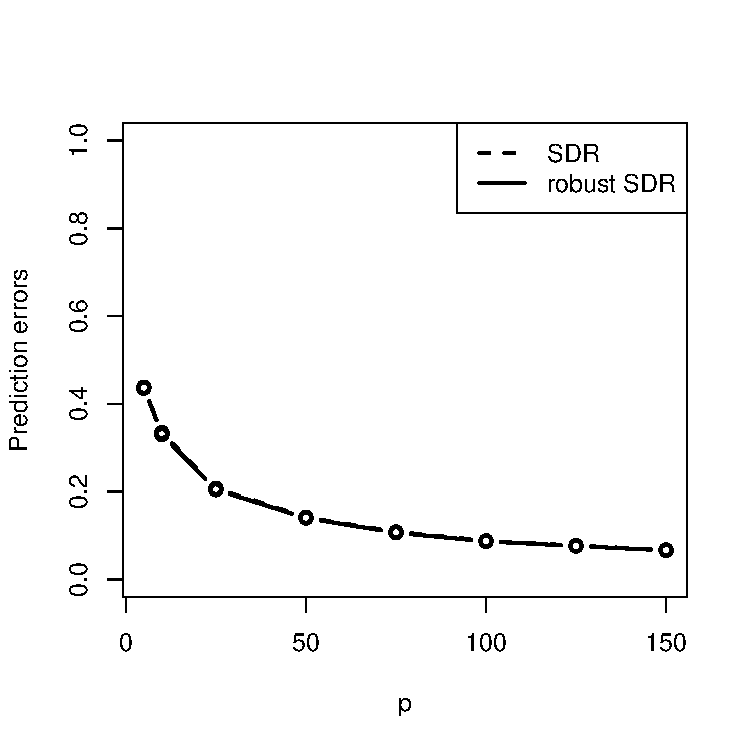
\includegraphics[width=0.35\textwidth]{SDRcomparison_noout}
	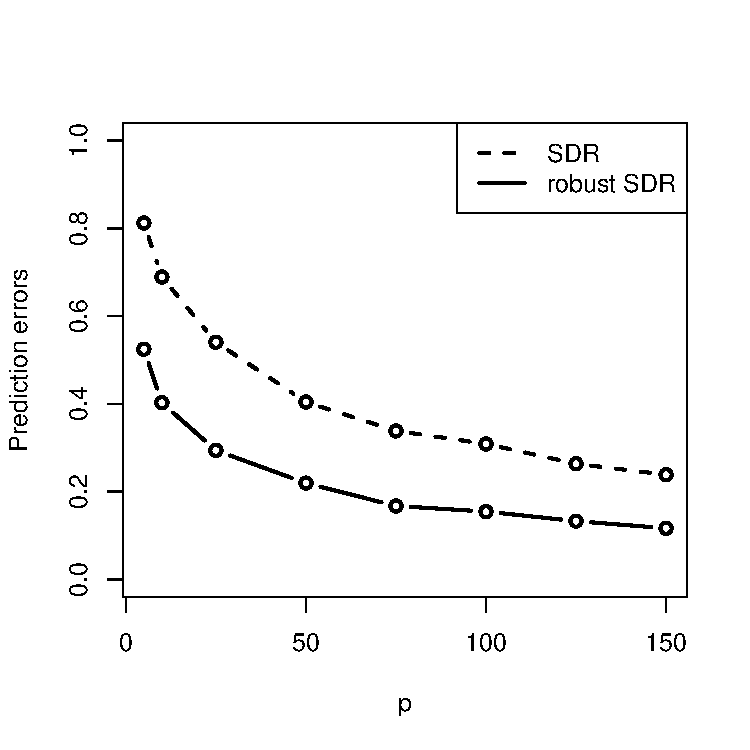
\includegraphics[width=0.35\textwidth]{SDRcomparison_out}
	\caption{Plot of the norm of influence function for first eigenvector of (a) sample covariance matrix, (b) SCM, (c) Tyler's scatter matrix and DCMs for (d) Halfspace depth, (e) Mahalanobis depth, (f) Projection depth for a bivariate normal distribution with $\bfmu = {\bf 0}, \Sigma = \diag(2,1)$}
	\label{fig:SDRfig}
\end{figure}

We formulate a robust version of the above procedure by estimating the quantities $\bfGamma, \bar\bfmu, \bfmu_y, \sigma^2$ by robust methods. Specifically, we take the following as their estimates:
%
\begin{itemize}
\item $\hat {\tilde \bfGamma}_d = $ first $d$ eigenvectors of the sample DCM;
%
\item $\hat \bfmu_s = $ spatial median of the rows of the data matrix $\BX_n$;
%
\item $\hat \bfmu_{s,y} = $ spatial median of the rows of $ \BX_y = \BX_n | Y=y$, for all $y \in S_Y$;
%
\item $\tilde\sigma^2 = \sum_{j=1}^p [\widehat{\text{MAD}}_Y (\BX_{Y,j} - \hat \mu_{s,j} - \hat {\tilde \bfgamma}_{d,j}^T \tilde \bfv_Y)]^2/p$, with $\hat {\tilde \bfGamma}_d = (\hat {\tilde \bfgamma}_{d,1}, ..., \hat {\tilde\bfgamma}_{d,p} )^T$, and MAD being the median absolute deviation.
\end{itemize}
%
The following simulation study using the same setup as in \citep{AdragniCook09} compares the performance of our robust SDR with the original method with or without the presence of bad leverage points in the covariate matrix $\BX_n$. For a fixed dimension $p$, we take $n=200, d=1$, generate the responses $Y$ as independent standard normal, and the predictors as $\BX_Y = \bfgamma^* v_Y^* + \bfepsilon$, with $\bfgamma^*_{p\times 1} = (1,...,1)^T, v_Y = Y + Y^2 + Y^3$ and $ \BV (\bfepsilon) = 25 \bfI_p$. We measure performance of both SDR models by their mean squared prediction error on another set of 200 observations generated similarly, and taking the average of these errors on 100 such training-test pair of datasets. Finally we repeat the whole setup for different choices of $p = 5,10,25,50,75,100,125,150$.

Panel (a) of \ref{fig:SDRfig} compares prediction errors using robust and maximum likelihood SDR estimates when the covariate matrix contains no outliers, and the two methods are virtually indistinguishable. We now introduce outliers in each of the 100 datasets by adding 100 to first $p/5$ coordinates of the first 10 samples in $\BX_n$, and repeat the analysis. Panel (b) of the figure shows that although our robust method performs slightly worse than the case when there were no outliers, it remains more accurate in predicting out-of-sample observations for all values of $p$. 
\section{Robust inference with functional data}
\label{section:fpcaSection}

Detection of anomalous observations is of importance in real-life problems involving functional data analysis, and functional PCA is a widely used tool in this setting. In this section we use robust principal components from the DCM for this purpose. We shall use the approach of \cite{BoenteBarrera15} for performing robust PCA on functional data using the estimated PCs from the DCM. Here we have a data matrix $\bfH$, that stores the values of a set of $n$ curves, say $ \cF = \{ f_1, \ldots , f_n  \} \in L^2[0,1]$, each observed at a set of common design points $\{ t_1, ..., t_m \} $. We model each of these functions as a linear combination of $p$ mutually orthogonal B-spline basis functions $\cD = \{ \delta_1, ..., \delta_p \}$. Following this, we map data for each of the functions onto the coordinate system formed by the spline basis:
%
\begin{equation}
T( \bfH; \cF, \cD)_{ij} = \sum_{l=2}^m f_i(t_l) \delta_j(t_l) (t_l - t_{l-1}); \quad 1 \leq i \leq n, 1 \leq j \leq p
\end{equation}
%
We now do depth-based PCA on the transformed $n \times p$ data matrix $T(\bfH; \cF, \cD) \equiv T(\bfH)$, and obtain the rank-$q$ approximation ($q \leq p$) of the $i^\text{th}$ observation using the robust $p \times q$ loading matrix $\tilde \bfP$ and robust $q \times 1$ score vector $\tilde\bfs_i$:
%
$$ \widehat T(\bfH)_i = \hat \bfmu_{s} + \tilde \bfP \tilde \bfs_i $$
%
with $\hat \bfmu_{s} $ being the spatial median of $T(\bfH)$. Then we transform this approximation back to the original coordinates: $\hat f_i (t_l) = \sum_{j=1}^p \widehat T(\bfH)_{ij} \delta_j (t_l)$.

We shall demonstrate the utility of our robust method for detecting functional outliers through two data examples. For any method of PCA with $k$ components on a dataset of $n$ observations and $p$ variables, the \textit{score distance} (SD) and \textit{orthogonal distance} (OD) for $i^\text{th}$ observation ($i=1,2,...,n$) are defined as:
%
$$
SD_i = \sqrt{ \sum_{j=1}^k \frac{s^2_{ij}}{\lambda_j}}; \quad OD_i = \| \bfx_i - \bfP\bfs_i^T \|
$$
%
where $\bfS = (\bfs_1, \ldots ,\bfs_n)^T \in \BR^{n\times k}$ is the score matrix, $\bfP \in \BR^{p\times k}$ the loading matrix, and $\lambda_1,\ldots ,\lambda_k$ are eigenvalues obtained from the PCA, and $\bfx_1,\ldots,\bfx_n$ are the $n$ observation vectors. From a practical standpoint, $SD_i$ can be interpreted as a weighted norm of the projection of the $i^\text{th}$ point on the hyperplane formed by first $k$ principal components, and $OD_i$ the orthogonal distance of point $i$ from that hyperplane. For outlier detection, following \cite{hubert05} we set the upper cutoff values for score distances at $\sqrt{\chi^2_{2,.975}}$ and orthogonal distances at $[\text{median}(OD^{2/3}) + \text{MAD}(OD^{2/3})\Phi^{-1}(0.975)]^{3/2}$, where $\Phi(.)$ is the standard normal cumulative distribution function.

\begin{figure}
%\captionsetup{justification=centering, font=footnotesize}
\begin{center}
\subfigure[]{\epsfxsize=.35\linewidth\epsfbox{Chapter-scatter/Elnino_functional1}}
\subfigure[]{\epsfxsize=.35\linewidth\epsfbox{Chapter-scatter/Octane_functional1}}\\

\subfigure[]{\epsfxsize=.35\linewidth\epsfbox{Chapter-scatter/Elnino_functional2}}
\subfigure[]{\epsfxsize=.35\linewidth\epsfbox{Chapter-scatter/Octane_functional2}}\\

\subfigure[]{\epsfxsize=.35\linewidth\epsfbox{Chapter-scatter/Elnino_functional3}}
\subfigure[]{\epsfxsize=.35\linewidth\epsfbox{Chapter-scatter/Octane_functional3}}\\
%\subfigure[]{\epsfxsize=0.35\linewidth \epsfbox{../Codes/SDRcomparison_out}}
\caption{Actual sample curves, their spline approximations and diagnostic plots respectively for El-Ni\~no (a,c,e) and Octane (b,d,f) datasets}
\label{fig:fPCAfig}
\end{center}
\end{figure}

We consider the El-Ni\~no data, which is part of a larger dataset on potential factors behind El-Ni\~no oscillations in the tropical pacific available in \url{http://www.cpc.ncep.noaa.gov/data/indices/}, as the first test case for outlier detection using our robust functional PCA. This records monthly average Sea Surface Temperatures from June 1970 to May 2004, and the yearly oscillations follow more or less the same pattern (see panel a of \ref{fig:fPCAfig}). Using a cubic spline basis with knots at alternate months starting in June gives a close approximation of the yearly time series data (panel c), and performing depth-based PCA with $q=1$ results in two points having their SD and OD larger than cutoff (panel e). These points correspond to the time periods June 1982 to May 1983 and June 1997 to May 1998 are marked by black curves in panels a and c), and pinpoint the two seasons with strongest El-Ni\~no events.

Our second application is on the Octane data, which consists of 226 variables and 39 observations \citep{esbensen94}. Each sample is a gasoline compound with a certain octane number, and has its NIR absorbance spectra measured in 2 nm intervals between 1100 - 1550 nm. There are 6 outliers here: compounds 25, 26 and 36-39, which contain alcohol. We use the same basis structure as the one in El-Ni\~no data here, and again the top robust PC turns out to be sufficient in identifying all 6 outliers (panels b, d and f of \ref{fig:fPCAfig}).
\section{Conclusion}\label{section:sec7}
\label{section:Conclusion}
In the above sections we elaborate on a proposed transformation based on the idea of combining sign functions in an inner product space and certain transformations of general peripherality functions defined using probability measures on the same space. Based on the conditions we impose in course of the chapter, we essentially end up using data depths as scalar multiples of the spatial sign in estimation and testing problems for the location parameter of an elliptical distribution in $\BR^p$, and using inverse depth functions for robust estimation of different components of its covariance matrix. As demonstrated by several simulation studies and data examples, in all these situations the use of this composite transformation vector brings about efficiency gains, as well as favorable robustness properties in terms of bounded influence functions and deviations from Gaussianity.

Regarding the multivariate rank transformation we propose, to be noted is the fact that the mapping $\bfX \mapsto \tilde \bfX$ is in fact one-to-one for elliptical distributions. Thus such rank vectors can possibly be used for inference based on transformation-retransformation type techniques (e.g. \cite{ChakrabortyChaudhuri96,ChakrabortyChaudhuriOja98}). We defer this to future research. Finally, while these rank vectors have excellent intuitive appeal in preserving the shape of a multivariate data cloud, it would be interesting to study the properties of transformations similar to \ref{eqn:kappaEqn} in general Hilbert spaces, as well as explore their applications in different data-analytic domains.
%\appendix
\section{Appendix}
%\renewcommand{\thesection}{\Alph{section}}
\subsection{Form of $\tilde\bfV (F)$}\label{subsec:appA}

First observe that for $F$ having covariance matrix $\Sigma = \bfGamma\bfLambda\bfGamma^T$,
%
$$ \tilde\bfV (F)  = (\bfGamma \otimes \bfGamma) \tilde\bfV (F_\bfLambda) (\bfGamma \otimes \bfGamma)^T$$
%
where $F_\bfLambda$ has the same elliptic distribution as $F$, but with covariance matrix $\bfLambda$. Now,
%
\begin{eqnarray*}
\tilde\bfV (F_\bfLambda) &=& \BE_\bfZ \left[ \ve \left\{ \frac{( D^- (\bfz, [\bfZ]))^2 \bfLambda^{1/2} \bfz\bfz^T \bfLambda^{1/2} }{ \bfz^T \bfLambda \bfz} - \tilde \bfLambda \right\} {\ve}^T \left\{ \frac{ (D^- (\bfz, [\bfZ] ) )^2 \bfLambda^{1/2} \bfz \bfz^T \bfLambda^{1/2} }{ \bfz^T \bfLambda \bfz} - \tilde \bfLambda \right\} \right]\\
&=& \BE \left[ \ve \left\{ ( D^- (\bfz, [\bfZ] ))^2 \BS( \bfLambda^{1/2} \bfz; {\bf 0} ) \right\} {\ve}^T \left\{ (D^- (\bfz, [\bfZ] ))^2 \BS( \bfLambda^{1/2}\bfz; \bf0) \right\} \right]\\
&& - \quad \ve( \tilde \bfLambda) {\ve}^T( \tilde \bfLambda )
\end{eqnarray*}

The matrix $\ve( \tilde\bfLambda) \ve^T(\tilde\bfLambda)$ consists of elements $\lambda_i\lambda_j$ at $(i,j)^\text{th}$ position of the $(i,j)^\text{th}$ block, and 0 otherwise. These positions correspond to variance and covariance components of on-diagonal elements. For the expectation matrix, all its elements are of the form $ \BE[ \sqrt{\lambda_a \lambda_b \lambda_c \lambda_d} z_a z_b z_c z_d . (D^- (\bfz, [\bfZ] ))^4 / (\bfz^T \bfLambda \bfz)^2]$, with $1 \leq a,b,c,d \leq p$. Since $(D^- (\bfz, [\bfZ] ))^4 / (\bfz^T \bfLambda \bfz)^2$ is even in $\bfz$, which has a circularly symmetric distribution, all such expectations will be 0 unless $a=b=c=d$, or they are pairwise equal. Following a similar derivation for spatial sign covariance matrices in \cite{magyar14}, we collect the non-zero elements and write the matrix of expectations:
%
$$ (\bfI_{p^2} + \bfK_{p,p}) \left\{ \sum_{a=1}^p \sum_{b=1}^p \tilde\gamma_{ab} (\bfe_a \bfe_a^T \otimes  \bfe_b \bfe_b^T) - \sum_{a=1}^p \tilde\gamma_{aa} (\bfe_a \bfe_a^T \otimes  \bfe_a \bfe_a^T) \right\} + \sum_{a=1}^p \sum_{b=1}^p \tilde\gamma_{ab} (\bfe_a \bfe_b^T \otimes  \bfe_a \bfe_b^T) $$
%
where $\bfI_k = (\bfe_1,...,\bfe_k), \bfK_{m,n} = \sum_{i=1}^m \sum_{j=1}^n \bfJ_{ij} \otimes \bfJ_{ij}^T$ with $\bfJ_{ij} \in \BR^{m \times n}$ having 1 as $(i,j)$-th element and 0 elsewhere, and $\tilde\gamma_{mn} = \BE[ \lambda_m \lambda_n z_m^2 z_n ^2 . (D^- (\bfz, [\bfZ] ))^4 / (\bfz^T \bfLambda \bfz)^2]; 1 \leq m,n \leq p$.

\paragraph{}Putting everything together, denote $\hat{\tilde \BS }(F_\bfLambda) = \sum_{i=1}^n ( D^-(\bfz_i, [\BZ_n]))^2 \BS( \bfLambda^{1/2} \bfz_i; \hat \bfmu_n)/n $. Then the different types of elements in the matrix $\tilde\bfV (F_\bfLambda)$ are as given below ($1 \leq a,b,c,d \leq p$):

\begin{itemize}
\item Variance of on-diagonal elements
%
$$ A\BV( \sqrt n \hat {\tilde s}_{aa} (F_\bfLambda)) = \BE \left[ \frac{(\tilde D^- (\bfz, [\bfZ]) )^4 \lambda_a^2 z_a^4}{(\bfz^T \bfLambda \bfz)^2} \right] - \tilde\lambda_{a}^2 $$

\item Variance of off-diagonal elements ($a \neq b$)
%
$$ A\BV( \sqrt n \hat {\tilde s}_{ab} (F_\bfLambda)) = \BE \left[ \frac{(D^- (\bfz, [\bfZ]))^4 \lambda_a \lambda_b z_a^2 z_b^2}{(\bfz^T \bfLambda \bfz)^2} \right] $$

\item Covariance of two on-diagonal elements ($a \neq b$)
%
$$ A\BV(\sqrt n \hat {\tilde s}_{aa} (F_\bfLambda), \sqrt n \hat{\tilde s}_{bb} (F_\bfLambda))
= \BE \left[ \frac{(D^- (\bfz, [\bfZ]))^4 \lambda_a \lambda_b z_a^2 z_b^2}{(\bfz^T \bfLambda \bfz)^2} \right] - \tilde\lambda_{a} \tilde\lambda_{b} $$

\item Covariance of two off-diagonal elements ($a \neq b \neq c \neq d$)
%
$$ A\BV(\sqrt n \hat {\tilde s}_{ab} (F_\bfLambda), \sqrt n \hat {\tilde s}_{cd} (F_\bfLambda)) = 0 $$

\item Covariance of one off-diagonal and one on-diagonal element ($a \neq b \neq c$)
%
$$ A\BV(\sqrt n \hat {\tilde s}_{ab} (F_\bfLambda), \sqrt n \hat {\tilde s}_{cc} (F_\bfLambda)) = 0 $$
\end{itemize}

\subsection{Asymptotics of eigenvectors and eigenvalues}
\label{subsection:appB}
The following result allows us to obtain asymptotic joint distributions of eigenvectors and eigenvalues of the sample DCM, provided we know the limiting distribution of the sample DCM itself:

\begin{Theorem} \label{Theorem:decomp} \citep{taskinen12}
Let $F_\bfLambda$ be an elliptical distribution with a diagonal covariance matrix $\bfLambda$, and $\hat \bfC$ be any positive definite symmetric $p \times p$ matrix such that at $F_\bfLambda$ the limiting distribution of $\sqrt n \ve(\hat \bfC - \bfLambda)$ is a $p^2$-variate (singular) normal distribution with mean zero. Write the spectral decomposition of $\hat \bfC$ as $\hat \bfC = \hat \bfP \hat\bfLambda \hat \bfP^T$. Then the limiting distributions of $\sqrt n \ve(\hat \bfP - \bfI_p)$ and $\sqrt n \ve( \hat\bfLambda - \bfLambda)$ are multivariate (singular) normal and
%
\begin{equation} \label{equation:decompEq}
\sqrt n \ve (\hat \bfC - \bfLambda)  = \left[ (\bfLambda \otimes \bfI_p) - (\bfI_p \otimes \bfLambda) \right] \sqrt n \ve (\hat \bfP - \bfI_p) + \sqrt n \ve (\hat \bfLambda - \bfLambda) + o_P(1)
\end{equation}
\end{Theorem}

The first matrix picks only off-diagonal elements of the LHS and the second one only diagonal elements. We shall now use this as well as the form of the asymptotic covariance matrix of the vec of sample DCM, i.e. $\tilde\bfV (F)$ to obtain limiting variance and covariances of eigenvalues and eigenvectors.

\begin{Corollary} \label{Corollary:eigendist}
Consider the sample DCM $ {\tilde \BS}(F) = \sum_{i=1}^n ( D^- (\bfx_i, [ \BX_n ] ))^2 \BS( \bfx_i; \hat\bfmu_n )/n $ and its spectral decomposition ${\tilde \BS}(F)= \widehat {\tilde \bfGamma} \widehat {\tilde \bfLambda} \widehat {\tilde \bfGamma}^T $. Then the matrices $\bfG = \sqrt n (\widehat {\tilde \bfGamma} - \bfGamma) $ and $\bfL = \sqrt n (\widehat {\tilde \bfLambda} - \tilde \bfLambda) $ have independent distributions. The random variable $\ve (\bfG)$ asymptotically has a $p^2$-variate normal distribution with mean ${\bf 0}_{p^2}$, and the asymptotic variance and covariance of different columns of $\bfG = (\bfg_1,...,\bfg_p)$ are as follows:
%
\begin{equation} \label{equation:DevEq}
A\BV(\bfg_i) = \sum_{k=1; k \neq i}^p \frac{1}{(\tilde \lambda_k - \tilde \lambda_i)^2} \BE \left[ \frac{(D^- (\bfz, [\bfZ]))^4 \lambda_i \lambda_k z_i^2 z_k^2}{(\bfz^T \bfLambda \bfz)^2} \right] \bfgamma_k \bfgamma_k^T
\end{equation}
%
\begin{equation}
A\BV(\bfg_i, \bfg_j) = - \frac{1}{(\tilde \lambda_i - \tilde \lambda_j)^2} \BE \left[ \frac{(D^- (\bfz, [\bfZ]))^4 \lambda_i \lambda_j z_i^2 z_j^2}{(\bfz^T \bfLambda \bfz)^2} \right] \bfgamma_j \bfgamma_i^T; \quad i \neq j
\end{equation}
%
where $\bfGamma = (\bfgamma_1,...,\bfgamma_p)$. The vector consisting of diagonal elements of $bfL$, say $\bfl = (\l_1,...,\l_p)^T$ asymptotically has a $p$-variate normal distribution with mean ${\bf 0}_p$ and variance-covariance elements:
%
\begin{eqnarray}
A\BV(l_i) &=& \BE \left[ \frac{(D^- (\bfz, [\bfZ]))^4 \lambda_i^2 z_i^4}{(\bfz^T \Lambda \bfz)^2} \right] - \tilde \lambda_i^2\\
A\BV(l_i, l_j) &=& \BE \left[ \frac{(D^- (\bfz, [\bfZ]))^4 \lambda_i \lambda_j z_i^2 z_j^2}{(\bfz^T \Lambda \bfz)^2} \right] - \tilde \lambda_i \tilde \lambda_j; \quad i \neq j
\end{eqnarray}
%
\end{Corollary}

%\begin{proof}[Proof of Theorem \ref{Theorem:decomp}]
%See \cite{taskinen12}
%\end{proof}

\begin{proof}[Proof of Corollary \ref{Corollary:eigendist}]
In spirit, this corollary is similar to Theorem 13.5.1 in \cite{anderson}. Due to the decomposition \ref{equation:decompEq} we have, for the distribution $F_\bfLambda$, the following relation between any off-diagonal element of $\tilde \BS(F_\bfLambda)$ and the corresponding element in the estimate of eigenvectors $\widehat{\tilde \bfGamma} (F_\bfLambda)$:

$$ \sqrt n \widehat{\tilde \gamma}_{ij} (F_\bfLambda) = \sqrt n \frac{{\tilde \BS}_{ij} (F_\bfLambda)}{\tilde \lambda_i - \tilde \lambda_j}; \quad i \neq j$$

So that for eigenvector estimates of the original $F$ we have
%
\begin{equation} \label{equation:app1}
\sqrt n (\widehat {\tilde \bfgamma}_{i} - \bfgamma_i) = \sqrt n \bfGamma (\widehat {\tilde \bfgamma}_{i}(F_\bfLambda) - \bfe_i ) = \sqrt n \left[ \sum_{k=1; k \neq i}^p \widehat {\tilde \gamma}_{ik}(F_\bfLambda)\bfgamma_k + (\widehat {\tilde \gamma}_{ii}(F_\bfLambda) - 1)\bfgamma_i \right]
\end{equation}
%
Now $\sqrt n (\widehat {\tilde \gamma}_{ii}(F_\bfLambda) - 1) =  o_P(1)$ and $A\BV(\sqrt n {\tilde \BS}_{ik}(F_\bfLambda), \sqrt n {\tilde \BS}_{il}(F_\bfLambda)) = 0$ for $k \neq l$, so the above equation implies
%
$$ A\BV(\bfg_i) = AVar (\sqrt n (\widehat {\tilde \bfgamma}_{i} - \bfgamma_i)) = \sum_{k=1; k \neq i}^p \frac{A\BV(\sqrt n {\tilde \BS}_{ik}(F_\bfLambda))}{(\tilde \lambda_i - \tilde \lambda_k)^2} \bfgamma_k \bfgamma_k^T $$
%

For the covariance terms, from \ref{equation:app1} we get, for $i \neq j$,
%
\begin{eqnarray*}
A\BV(\bfg_i, \bfg_j) &=& A\BV(\sqrt n (\widehat {\tilde \bfgamma}_{i} - \bfgamma_i), \sqrt n (\widehat {\tilde \bfgamma}_{j} - \bfgamma_j))\\
&=& A\BV \left( \sum_{k=1; k \neq i}^p \sqrt n \widehat {\tilde \gamma}_{ik}(F_\bfLambda)\bfgamma_k, \sum_{k=1; k \neq j}^p \sqrt n \widehat {\tilde \gamma}_{jk}(F_\bfLambda)\bfgamma_k \right)\\
&=& A\BV \left( \sqrt n \widehat {\tilde \gamma}_{ij}(F_\bfLambda)\bfgamma_j, \sqrt n \widehat {\tilde \gamma}_{ji}(F_\bfLambda)\bfgamma_i \right)\\
&=& - \frac{A\BV(\sqrt n {\tilde \BS}_{ij}(\Lambda))}{(\tilde \lambda_i - \tilde \lambda_j)^2} \bfgamma_j \bfgamma_i^T
\end{eqnarray*}
%
The exact forms given in the statement of the corollary now follows from the  Form of $\tilde \bfV(F)$ in \ref{subsec:appA}.

\paragraph{}For the on-diagonal elements of $\tilde \BS(F_\bfLambda)$ Theorem \ref{Theorem:decomp} gives us $ \sqrt n \hat\tilde \lambda_i (F_\bfLambda) = \sqrt n {\tilde \BS}_{ii}(F_\bfLambda)$ for $i = 1,...,p$. Hence

\begin{eqnarray*}
A\BV(l_i) &=& A\BV(\sqrt n \hat\tilde \lambda_i - \sqrt n \tilde \lambda_i)\\
&=& A\BV(\sqrt n \hat\tilde \lambda_i (F_\bfLambda) - \sqrt n \tilde \lambda_i(F_\bfLambda))\\
&=& A\BV(\sqrt n {\tilde \BS}_{ii}(F_\bfLambda))
\end{eqnarray*}

A similar derivation gives the expression for $A\BV(l_i,l_j); i \neq j$. Finally, since the asymptotic covariance between an on-diagonal and an off-diagonal element of $\tilde \BS(F_\bfLambda)$, it follows that the elements of $\bfG$ and diagonal elements of $\bfL$ are independent.
\end{proof}

\subsection{Proofs}
\label{subsection:appC}

\begin{proof}[Proof of Proposition \ref{proposition:SignTest}]
Under contiguous alternatives $H_0: \bfmu = \bfmu_0$, the weighted sign test statistic $T_{n,w}$ has mean $\BE (w(\bfZ) \bfS (\bfZ))$. For spherically symmetric $\bfZ$, $w(\bfZ)$ depends on $\bfZ$ only through its norm. Since $\| \bfZ \|$ and $\bfS(\bfZ)$ are independent, we get $\BE (w(\bfZ) \bfS (\bfZ)) = \BE w(\bfZ). \BE \bfS (\bfZ)$. The same kind of decomposition holds for $\BV(w(\bfZ) \bfS(\bfZ))$.

We can now simplify the approximate local power $\beta_{n,w}$ of the level-$\alpha$ ($0 < \alpha < 1$) test based on $T_{n,w}$:
%
\begin{eqnarray*}
\beta_{n,w} &=& K_p \left( \chi^2_{p,\alpha} + n \times \right.\\
&& \left.  (\BE (w(\bfZ) \bfS (\bfZ))^T [ \BE (w^2(\bfZ) \bfS (\bfZ) \bfS (\bfZ)^T) ]^{-1} (\BE (w(\bfZ) \bfS (\bfZ)) \right)\\
&=& K_p \left( \chi^2_{p,\alpha} + \frac{\BE^2 w(\bfZ)}{\BE w^2(\bfZ)}. \BE \bfS(\bfZ)^T [\BV \bfS( \bfZ)]^{-1} \BE \bfS( \bfZ) \right)
\end{eqnarray*}
%
where $K_p$ and $\chi^2_{p,\alpha}$ are distribution function and upper-$\alpha$ cutoff of a $\chi^2_p$ distribution, respectively. Since $\BE^2 w(\bfZ) \leq \BE w(\bfZ)$, $\beta_{n,w}$ the largest possible value of $\beta_{n,w}$ is $K_p ( \chi^2_{p,\alpha} + \BE\bfS(\bfZ)^T [\BV \bfS(\bfZ)]^{-1} \BE\bfS(\bfZ) )$, the approximate power of the unweighted sign test statistic. Equality is of course achieved when $w(\bfZ)$ is a constant independent of $\bfZ$.
\end{proof}

\begin{proof}[Proof of corollary \ref{Corollary:wsmCorollary}]
Since $\bfepsilon \sim \mathcal{E}(\bfmu, k\bfI_p, g)$, $r = \| \bfepsilon \|$ and $ \bfS( \bfepsilon)$ are independent. Also $w( \bfepsilon) = f(r)$. Thus
%
\begin{eqnarray*}
\bfA_w &=& \BE \left( \frac{ f(r)}{r } \right) \BE ( \bfI_p - \bfS ( \bfepsilon) \bfS (\bfepsilon)^T);\\
\bfB_w &=& \BE f^2 (r) \BE ( \bfS ( \bfepsilon) \bfS (\bfepsilon)^T)
\end{eqnarray*}
%
We conclude by substituting these in \ref{eqn:AREEqn}.
\end{proof}

\begin{proof}[Sketch of proofs for equations \ref{eqn:hdtest1} and \ref{eqn:hdtest2}]

A first step to obtain asymptotic normality for the high-dimensional location test statistic $C_{n,w}$ is obtaining an equivalent result of Lemma 2.1 in \cite{WangPengLi15}:

\begin{Lemma}\label{Lemma:HDlemma21} Under the conditions

\noindent\textbf{(C1)}$\text{Tr}(\bfSigma^4) = o(\text{Tr}^2(\bfSigma^2)) $,

\noindent\textbf{(C2)}$\text{Tr}^4(\bfSigma) / \text{Tr}^2(\bfSigma^2) \exp[ - \text{Tr}^2(\bfSigma) / 128p \lambda^2_{\max}(\bfSigma) ] = o(1)$
\vspace{1em}

\noindent when $H_0$ is true we have
%
\begin{eqnarray}
\BE[ (\bfepsilon_{w1}^T \bfepsilon_{w2})^4 ] &=& O(1) \BE^2[ (\bfepsilon_{w1}^T \bfepsilon_{w2})^2 ]\\
\BE[ (\bfepsilon_{w1}^T B_w \bfepsilon_{w1})^2 ] &=& O(1) \BE^2[ (\bfepsilon_{w1}^T B_w \bfepsilon_{w1})^2 ]\\
\BE[ (\bfepsilon_{w1}^T B_w \bfepsilon_{w2})^2 ] &=& o(1) \BE^2[ (\bfepsilon_{w1}^T B_w \bfepsilon_{w1})^2 ]
\end{eqnarray}
%
with $\bfepsilon \sim \mathcal \BE({\bf 0}_p, \bfLambda, g)$ and $\bfepsilon_w = w(\bfepsilon) \bfS(\bfepsilon)$.
\end{Lemma}
%
A proof of this lemma is derived using results in section 3 of \cite{ElKaroui09}, noticing that any-scalar valued 1-Lipschitz function of $\bfepsilon_w$ is a $M_w$-Lipschitz function of $\bfS(\bfepsilon)$, with $M_w = \sup_\bfepsilon w(\bfepsilon)$. Same steps as in the proof of Theorem 2.2 in \cite{WangPengLi15} follow now, using the lemma above in place of Lemma 2.1 therein, to establish asymptotic normality of $C_{n,w}$ under $H_0$.

To derive the asymptotic distribution under contiguous alternatives we need the conditions (C3)-(C6) in \cite{WangPengLi15}, as well as slightly modified versions of Lemmas A.4 and A.5:

\begin{Lemma}
Given that condition (C3) holds, we have $\lambda_{\max} (\bfB_w) \leq 2 \frac{\lambda_{\max}}{\text{Tr} (\bfSigma)} (1+o(1))$.
\end{Lemma}

\begin{Lemma}
Define $\bfD_w = \BE \left[ \frac{w^2(\bfepsilon)}{\| \bfepsilon \|^2} (\bfI_p - \bfS(\bfepsilon) \bfS(\bfepsilon)^T )\right] $. Then $\lambda_{\max} (\bfA_w) \leq \BE( w(\bfepsilon)/\| \bfepsilon \|)$ and $\lambda_{\max} (\bfD_w) \leq \BE( w(\bfepsilon)/\| \bfepsilon \|)^2$. Further, if (C3) and (C4) hold then $\lambda_{\min} (\bfA_w) \geq \BE( w(\bfepsilon)/\| \bfepsilon \|)(1+o(1))/\sqrt 3$.
\end{Lemma}
%
The proof now exactly follows steps in the proof of theorem 2.3 in \cite{WangPengLi15}, replacing vector signs by weighted signs, using the fact that $w(\bfepsilon)$ is bounded above by $M_w$ while applying conditions (C5)-(C6) and lemmas A.1, A.2, A.3, and finally using the above two lemmas in place of lemmas A.4 and A.5 respectively.
\end{proof}

\begin{proof}[Proof of Theorem  \ref{Theorem:covform}]
The proof follows directly from writing out the expression of $\BV( \tilde \bfX)$:
%
\begin{eqnarray*}
\BV( \tilde\bfX) &=& \BE(\tilde\bfX \tilde\bfX^T) - \BE \tilde\bfX \BE \tilde\bfX^T\\
&=& \bfGamma . \BE \left[ ( D^- (\bfz, [\bfZ]) )^2 \frac{\|\bfz\|^2}{\| \bfLambda^{1/2}\bfz\|} \bfLambda^{1/2} \bfS(\bfz) \bfS(\bfz)^T \bfLambda^{1/2} \right] \bfGamma^T - {\bf 0}_p {\bf 0}_p^T\\
&=& \bfGamma .\BE \left[ (D^- (\bfz, [\bfZ]))^2 \frac{\bfLambda^{1/2} \bfz \bfz^T \bfLambda^{1/2}}{\bfz^T \bfLambda \bfz} \right] \bfGamma^T
\end{eqnarray*}
%
\end{proof}

\begin{proof}[Proof of Lemma \ref{Lemma:lemma1}]
For two positive definite matrices $\bfA, \bfB$, we denote by $\bfA > \bfB$ that $\bfA - \bfB$ is positive definite. Also, denote
%
$$ \BS_n = \sqrt n \left[ \frac{1}{n} \sum_{i=1}^n \left| ( D^- (\bfx_i, [ \BX_n]))^2  - ( D^- (\bfx_i, [\bfX]))^2 \right| \BS (\bfx_i; \hat\bfmu_n) \right] $$
%
%Consider now the quantity $\bft^T S_n \bft$, where $\bft \in \mathbb{R}^p$. Now applying Cauchy-Schwarz inequality we shall have
%%
%\begin{eqnarray}\label{eqn:AppEqn1}
%\frac{(\bft^T S_n \bft)^2}{n} & = & \left[ \frac{1}{n} \sum_{i=1}^n \left| (\tilde D^{n} _\bfX (\bfx_i))^2  - (\tilde D_\bfX (\bfx_i))^2 \right|^2  \bft^T \BS( \bfx_i; \hat\bfmu_n) \bft \right]^2 \notag\\
%& \leq & \left[ \frac{1}{n} \sum_{i=1}^n \left| (\tilde D^{n} _\bfX (\bfx_i))^2  - (\tilde D_\bfX (\bfx_i))^2 \right|^2 \right] \left[ \frac{1}{n} \left( \sqrt n.\frac{1}{n} \sum_{i=1}^n  \BS( \bfx, \hat\bfmu_n) \right) \right]
%\end{eqnarray}
%%
%with $\hat S_n = \sum_{i=1}^n \BS( \bfx_i, \hat\bfmu_n)/ \sqrt n$.
Due to the assumption of uniform convergence, given $\epsilon>0$ we can find $N \in \mathbb{N}$ such that
%
\begin{equation}
\label{equation:lemma1eq}
| (  D^- (\bfx_i, [ \BX_{n_1}]) )^2 - ( D^- (\bfx_i, [\bfX]) )^2 | < \epsilon
\end{equation}
%
for all $n_1 \geq N; i = 1,2,...,n_1$. This implies
%
\begin{eqnarray}
\label{eqn:lemma1eq2}
\BS_{n_1} &< & \epsilon \sqrt{n_1} \left[ \frac{1}{n_1} \sum_{i=1}^{n_1} \BS( \bfx_i; \hat\bfmu_{n_1}) \right]\notag\\
&=& \epsilon \sqrt{n_1} \left[ \frac{1}{n_1} \sum_{i=1}^{n_1} \left\{ \BS( \bfx_i; \hat\bfmu_{n_1}) -  \BS (\bfx_i; \bfmu) \right\} + \frac{1}{n_1} \sum_{i=1}^{n_1} \BS( \bfx_i; \bfmu) \right]
\end{eqnarray}

We now construct a sequence of positive definite matrices $\{a_k (\bfB_k + \bfC_k) : k \in \mathbb N\} $ so that
%
$$ a_k = \frac{1}{k}, \quad \bfB_k = \sqrt{N_k} \left[ \frac{1}{N_k} \sum_{i=1}^{N_k} \left\{ \BS( \bfx_i; \hat\bfmu_{N_k}) - \BS( \bfx_i; \bfmu) \right\} \right]$$
$$\quad \bfC_k = \sqrt{N_k} \left[ \frac{1}{N_k} \sum_{i=1}^{N_k} \BS( \bfx_i; \bfmu) \right] $$
%
where $N_k \in \mathbb N$ gives the relation \ref{equation:lemma1eq} in place of $N$ when we take $\epsilon = 1/k$. Under conditions $ \BE \|\bfx - \bfmu\|^{-3/2} < \infty $ and $\sqrt n (\hat\bfmu_n - \bfmu) = O_P(1)$, the sample SCM with unknown location parameter $\hat\bfmu_n$ has the same asymptotic distribution as the SCM with known location $\bfmu$ \citep{durre14}, hence $\bfB_k = o_P(1)$. Also $\bfC_k = O_P(1)$, thus $a_k (\bfB_k + \bfC_k) \stackrel{P}{\rightarrow} 0$ as $k \raro \infty$.

Now \ref{eqn:lemma1eq2} implies that for any $\epsilon_1 > 0$, $\BS_{N_k} > \epsilon_1 \Rightarrow a_k (\bfB_k + \bfC_k) > \epsilon_1$, which means $ P(\BS_{N_k} > \epsilon_1) < P(a_k (\bfB_k + \bfC_k) > \epsilon_1)$. Hence the subsequence $\{\BS_{N_k}\} \stackrel{P}{\rightarrow} 0$. Since the main sequence $\{\BS_n\}$ is bounded below by 0, this implies $\{\BS_n\} \stackrel{P}{\rightarrow} 0$. Finally, we have that
%
\begin{eqnarray}
\sqrt n \left[
\frac{1}{n} \sum_{i=1}^n ( D^- (\bfx_i, [ \BX_n]) )^2 \BS( \bfx_i; \hat\bfmu_n) -
\frac{1}{n} \sum_{i=1}^n ( D^- (\bfx_i, [\bfX]) )^2 \BS( \bfx_i; \bfmu) \right] &\leq & \hspace{1em} \notag\\
\BS_n +  \max_\bfx (D ( \bfx, [\bfX]))^2 . \sqrt{n} \left[ \frac{1}{n} \sum_{i=1}^{n} \left\{ \BS( \bfx_i; \hat\bfmu_{n}) - \BS( \bfx_i; \bfmu) \right\} \right] &&
\end{eqnarray}
%
The second summand on the right hand side is $o_P(1)$ due to \cite{durre14} as mentioned before, so we have the needed.
\end{proof}

\begin{proof}[Proof of Theorem \ref{Theorem:rootn}]
The quantity in the statement of the theorem can be broken down as:
%
\begin{eqnarray*}
\sqrt n \left[ \ve \left\{ \frac{1}{n} \sum_{i=1}^n ( D^- (\bfx_i, [\bfX]))^2 \BS(\bfx_i; \hat\bfmu_n) \right\} - \ve \left\{ \frac{1}{n} \sum_{i=1}^n ( D^- (\bfx_i, [\bfX] ) )^2 \BS( \bfx_i; \bfmu) \right\} \right] +\\
\sqrt n \left[ \ve \left\{ \frac{1}{n} \sum_{i=1}^n ( D^- (\bfx_i, [\bfX] ) )^2 \BS( \bfx_i; \bfmu) \right\} - \BE \left[ \ve \left\{ ( D^- (\bfx, [\bfX] ) )^2 \BS (\bfx; \bfmu) \right \} \right] \right]
\end{eqnarray*}
%
The first part goes to 0 in probability by Lemma \ref{Lemma:lemma1}, and applying Slutsky's theorem we get the required convergence.
\end{proof}

\begin{proof}[Proof of Theorem \ref{Thm:pluginSigma}]
We are going to prove the following:
%
\begin{enumerate}
\item $\| \widehat{\tilde \bfGamma} - \bfGamma \|_F \stackrel{P}{\rightarrow} 0$, and

\item $\| \widehat{\bfLambda} - \bfLambda \|_F \stackrel{P}{\rightarrow} 0$
\end{enumerate}
%
as $n \rightarrow \infty$. For (1), we notice $\sqrt n \ve (\widehat{\tilde \bfGamma} - \bfGamma)$ asymptotically has a (singular) multivariate normal distribution following Corollary \ref{Corollary:eigendist}, so that $\| \widehat {\tilde \bfGamma} - \bfGamma \|_F = O_P(1/\sqrt n)$ using Prokhorov's theorem.

It is now enough to prove convergence in probability of the individual eigenvalue estimates $\hat\lambda_i; i = 1,...,p$. For this, define estimates $\hat \lambda^*_i$ as median-of-small-variances estimator of the \textit{true} score vectors $\bfGamma^T \BX_n$. For this we have
%
\begin{equation}\label{eqn:PluginSigmaProof1}
| \hat \lambda^*_i - \lambda_i | \stackrel{P}{\rightarrow} 0
\end{equation}
%
using Theorem 3.1 of \cite{Minsker15}, with $\mu = \lambda_i$. Now $ \hat{\lambda}_i = \text{med}_j (\BV( \BX_{G_j}^T \widehat{ \tilde \bfgamma}_{i} ))$ and $\hat \lambda^*_i = \text{med}_j (\BV( \BX_{G_j}^T \bfgamma_i )) $, so that
%
\begin{eqnarray*}
| \hat {\lambda}_i - \hat \lambda^*_i | &\leq & \text{med}_j \left[ \BV( \BX_{G_j}^T ( \widehat{\tilde\bfgamma}_{i} - \bfgamma_i) ) \right]
\\ &\leq & \| \widehat{\tilde\bfgamma}_{i} - \bfgamma_i \|^2 \text{med}_j  \left[ \text{Tr} (\BV( \BX_{G_j})) \right]
\end{eqnarray*}
%
using Cauchy-Schwarz inequality. Combining the facts $ \| \widehat{\tilde\bfgamma}_{i} - \bfgamma_i \| = O_P(1/\sqrt n)$ and $ \text{med}_j  [ \text{Tr} (\BV( \BX_{G_j})) ] \stackrel{P}{\rightarrow} \text{Tr}(\bfSigma)$ \citep{Minsker15} with \ref{eqn:PluginSigmaProof1}, we get the needed.

\end{proof}

%% Depth-based multitask regression
\chapter{Nonconvex Penalized Regression using Depth-based Penalty}
\label{chapter:regression-chapter}
%
\section{Introduction}

Consider the multitask linear regression model:
%
$$ \bfY = \bfX \bfB + \bfE $$
%
where $\bfY \in \mathbb R^{n\times q}$ is the matrix of responses, and $\bfE$ is $n\times q$ the noise matrix: each row of which is drawn from $\mathcal{N}_q ({\bf 0}_q, \bfSigma)$ for a $q \times q$ positive definite matrix $\bfSigma$. We are interested in sparse estimates of the coefficient matrix $\bfB$ through solving penalized regression problems of the form
%
\begin{equation}\label{eqn:penEqn}
\min_\bfB \Tr \{ (\bfY - \bfX\bfB)^T ( \bfY - \bfX\bfB) \} + P_\lambda(\bfB)
\end{equation}
%
The frequently studied classical linear model may be realized as a special case of this 
for $q = 1$, where given a size-$n$ sample of random responses $\bfy = (y_1, y_2, ..., y_n)^T$ and $p$-dimensional predictors $\bfX = (\bfx_1, \bfx_2, ...,\bfx_n)^T$, the 
above model may now be written as:
%
$$
\bfy = \bfX \bfbeta + \bfepsilon; \quad \bfepsilon = (\epsilon_1,...,\epsilon_n)^T \sim \mathcal N_n ({\bf 0}_n, \sigma^2\bfI_p).
$$
%

Here the typical objective is to estimate the parameter vector $\bfbeta$ by minimizing $\sum_{i=1}^n \rho ( y_i - \bfx_i^T \bfbeta)$, for some loss function $\rho(.)$. Selecting important variables in this setup is often significant from an inferential and predictive perspective it is generally achieved by obtaining an estimate of $\bfbeta$ that minimizes a linear combination of the loss function and a `penalty' term $P(\bfbeta) = \sum_{j=1}^p p(|\beta_j|)$, instead of only the loss function:
%
\begin{equation}\label{eqn:eqn01}
\hat\bfbeta_n = \argmin_\bfbeta \left[ \sum_{i=1}^n \rho ( y_i - \bfx_i^T \bfbeta) + \lambda_n P(\bfbeta) \right]
\end{equation}
%
where $\lambda_n$ is a tuning parameter depending on sample size. The penalty term is generally a measure of model complexity, providing a control against overfitting. Using a $l_0$ norm as penalty at this point, i.e. $p(z) = \BI_{z \neq 0}$, gives rise to the information criterion-based paradigm of statistical model selection, which goes back to the Akaike Information Criterion (AIC: \cite{Akaike70}). Owing to the intractability of this problem due to an exponentially growing model space, researchers have been exploring the use of functions that are non-differentiable at the origin as $p(.)$. This dates back to the celebrated LASSO \citep{Tibshirani96} which uses $l_1$ norm, adaptive LASSO \citep{Zou06} that reweights the coordinate-wise LASSO penalties based on Ordinary Least Square (OLS) estimate of $\bfbeta$, and \cite{FanLi01,CHZhang10} who used non-convex penalties to limit influence of large entries in the coefficient vector $\bfbeta$, resulting in improved estimation. Further, \cite{ZouLi08} and \cite{WangKimLi13} provided efficient algorithms for computing solutions to the nonconvex penalized problems.

Two immediate extensions of the univariate-response penalized sparse regression paradigm are group-wise penalties and multivariate penalized regression. Applying penalties at variable group level instead of individual variables gives rise to Group LASSO \citep{BakinThesis99}. From an application perspective, this utilizes additional relevant information on the natural grouping of predictors: for example multiple correlated genes, or blockwise wavelet shrinkage \citep{AntoniadisFan01}. On the other hand, for multitask regression, penalizing at the coefficient matrix-level results in better estimation and prediction performance compared to performing $q$ separate LASSO regressions to recover its corresponding columns \citep{RothmanEtal10}.

Compared to sparse single-response regression where the penalty term can be broken down to elementwise penalties, in the multivariate response  scenario we need to consider two levels of sparsity. The first level is recovering the set of predictors having non-zero effects on all the responses, as well as estimating their values. Assuming the coefficient matrix $\bfB \in \mathbb R^{p \times q}$ is made of rows $(\bfb_1,...,\bfb_p)^T$, this means determining the set $\bigcup_k \cS_k$, with $\cS_k := \{ k: b_{jk} \neq 0, j = 1, 2, ..., p \}$.  This is called \textit{support union recovery}, and is more effective in recovering non-zero elements of $\bfB$ compared to the na\"ive approach of performing $q$ separate sparse regularized regressions and combining the results \citep{ObozinskiEtal11}. The second level of sparsity is concerned with recovering non-zero elements \textit{within} the non-zero rows obtained from the first step. Our method addresses both of these issues.

Specifically, we consider the case of performing support union recovery by considering the inverse depth functions introduced in \ref{chapter:scatter-chapter} as row-level regularizers: $P_\lambda(\bfB) = \sum_{j=1}^p \lambda D^- (\bfb_j, F)$ where $F$ is some probability distribution fixed beforehand. \ref{sec:regression-sec2} motivates the use of a general depth-based regularization scheme in the multitask regression setup. From \ref{sec:regression-sec3} onward we choose to concentrate on the scenario when $D^- (\bfb_j, F) = p_{,F} (\|\bfb_j\|_2)$, i.e. the row-level penalty is a potentially nonconvex scalar-valued function of the row-norm. This automatically tempers the effects of large regression coefficients in the case of general  $q$-dimensional response: which is not the case for methods based on $l_1$-norm penalization, e.g. Lasso. We derive asymptotic results ensuring support union recovery, as well as provide an iterative algorithm for calculating the corresponding penalized estimator. We also show that a simple corrective thresholding on elements of the first level row-sparse estimator ensures sparse recovery of within-row elements as well. Additional theoretical results in the orthogonal design case are discussed in \ref{sec:regression-sec4}, and simulation experiments are presented to compare our algorithm with other methods in \ref{sec:regression-sec5}. We present a data application of the algorithm in \ref{sec:regression-sec6}, followed by conclusions. \ref{section:regression-sec8} contains proofs of our theoretical results.
\section{Depth-based regularization}
\label{sec:regression-sec2}
We incorporate measures of data depth as a row-level penalty function in \ref{eqn:penEqn}. Specifically, we estimate the coefficient matrix $\bfB$ by solving the following constrained optimization problem:
%
\begin{equation}\label{eqn:eqn02}
\hat\bfB = \argmin_\bfB \left[ \Tr \{ (\bfY - \bfX\bfB)^T ( \bfY - \bfX\bfB) \} + \lambda_n \sum_{j=1}^p P ( \bfb_j, F) \right]
\end{equation}
%
where $P ( \bfb_j, F)$ is a function that measures the peripherality of the $j$-th row of $\bfB$ with respect to a fixed probability distribution $F$, as defined in \ref{chapter:scatter-chapter}. We refer to $F$ as the \textit{reference distribution}, and consider it fixed in the estimation process. In multitask learning, any additive penalty function of the form $P_\lambda (\bfB) = \sum_{j=1}^p \lambda p( \bfb_j)$ regularizes individual rows of the coefficient matrix by providing a control over their distance from the origin ${\bf 0}_q$ through some norm (e.g. the $l_1/l_q$ penalty: \cite{NeghabanWainwright11}), or a combination of norms (e.g. the Adaptive Multi-task Elastic-Net: \cite{ChenEtal12}). Through \ref{eqn:eqn02} we attempt to generalize this notion by proposing to regularize using the `distance' from a \textit{probability distribution} centered at the origin. Of course, any existing method of norm-based regularization arises as a special case by by using the norm (or combination of norms) as the peripherality function and taking as $F$ the degenerate distribution centered at ${\bf 0}_q$. While it is possible to use any peripherality function (or outlyingness functions, in the spirit of \cite{zuo00}) for this purpose, of special interest is the case of \textit{inverse depth} functions: $P(\bfx, F) = D^- (\bfx, F)$. Such functions essentially invert the funnel-shaped contour of the corresponding depth function (\ref{fig:depthplot}). This immediately results in row-wise nonconvex penalties, where the penalty sharply increases for smaller entries inside the row but is bounded above for large values. This is easy to visualize for $p=1$, which we show in panel a of \ref{fig:fig1}. This serves as our motivation of using data depth in regularized multitask regression.
\section{The LARN algorithm}
\label{sec:regression-sec3}

\subsection{Formulation}\label{subsec:subsec31}
The reference distribution $F$ is pivotal in the estimation problem in \ref{eqn:eqn02}. While we believe that there is scope for a significant amount of theoretical analysis on the implications of different choices of $F$ and its potential connections to Bayesian regularized support union recovery in multitask regression, here we shall work within a simplified setup. Specifically we assume that

\vspace{1em}
\noindent\textbf{(A1)} The distribution $F$ is spherically symmetric.
\vspace{1em}

\noindent This is a fair assumption to make from a frequentist perspective, as we do not possess any extra information about the $q$ responses being different from one another. Since $F$ is spherically symmetric, depth at a point $\bfb$ becomes a function of $r = \| \bfb\|_2$ only, due to the affine invariance of $D(.,F)$. In this situation, several depth functions have closed-form expressions: e.g. when $D$ is projection depth and $F$ is a $p$-variate standard normal distribution, $D(\bfb_j, F) = c / (c + \| \bfb_j \|); c = \Phi^{-1}(3/4)$ \citep{zuo03}, while for halfspace depth and any known $F$, $D(\bfb_j, F) = 1 - F_1(\| \bfb_j \|)$, $F_1$ being any univariate marginal of $F$ (immediate from the definition of halfspace depth). Hence, the computational burden of calculating depths for rows of $\bfB$ becomes trivial.

\begin{figure}
%\captionsetup{justification=centering, font=footnotesize}
\vspace{-2em}
\begin{center}
%\subfigure[]{\epsfxsize=0.31\linewidth \epsfbox{Chapter-regression/depthplot_cropped}}
\subfigure[]{\epsfxsize=0.31\linewidth \epsfbox{Chapter-regression/penalties1}}
\subfigure[]{\epsfxsize=0.31\linewidth \epsfbox{Chapter-regression/threslarn}}
\vspace{-1em}
\caption{(a) Comparison of L1 and SCAD \citep{FanLi01} penalty functions with univariate halfspace depth: inverting the depth function helps obtain the nonconvex shape of the penalty function in the inverse depth; (b) Univariate thresholding rule for the LARN estimate assuming halfspace depth and max definition of inverse depth(see \ref{sec:regression-sec4})}
\label{fig:fig1}
\end{center}
\end{figure}

Because of the way we define inverse depth functions, the above holds for inverse depth functions $D^-(., F)$ as well. Thus we can write that $D^-(\bfb_j, F) = p_F (r_j)$ for some scalar-valued function $p_F(.)$. Any superscript or subscript in $\bfB$ or $\bfb_j$ will be passed accordingly to $r_j$. At this point we shall make the following technical assumption on $p_F(.)$:

\vspace{1em}
\noindent\textbf{(A2)} The function $p_F(r)$ is concave in $r$, and continuously differentiable at every $r \neq 0$.
\vspace{1em}

\noindent In general depth functions are assumed to have convex contours \citep{MoslerChapter13}, which implies quasi-concavity. Nevertheless, several depth functions adhere to concavity owing to their simplified closed forms for spherical distribution (e.g. halfspace depth and projection depth in the last paragraph). Continuous differentiability except at the origin, which is essential for admitting a sparse solution eventually, arises because of the same reason.

Keeping the above setup in mind, we now consider the first-order Taylor series approximation of the overall penalty function:
%
\begin{eqnarray}
\hspace{-1em} P_{\lambda.F} (\bfB) & := & \lambda \sum_{j=1}^p p_F (r_j) \notag\\
& \simeq & \lambda \sum_{j=1}^p \left[ p_F (r_j^*) + p'_F (r_j^*) ( r_j - r_j^*) \right]\label{eqn:majorizeEqn}
\end{eqnarray}
%
for any $\bfB^*$ close to $\bfB$, and $r_j = \| \bfb_j \|_2, r_j^* = \| \bfb_j^* \|_2; j = 1,2,...,p$.

Thus, given a starting solution $\bfB^*$ close enough to the original coefficient matrix, $P_{\lambda.F} (\bfB)$ is approximated by its conditional counterpart, say $P_{\lambda.F} (\bfB | \bfB^*)$. Following this a penalized maximum likelihood estimate for $\bfB$ can be obtained using the iterative algorithm below:
%
\begin{enumerate}
\item Take as starting value $\bfB^{(0)} = \hat \bfB
_{\text{LS}} = (\bfX^T \bfX)^- \bfX^T \bfY$, i.e. the least square estimate of $\bfB$, set $k=0$;

\item Calculate the next iterate by solving the penalized likelihood:
%
\begin{align}\label{eqn:mapEqn}
 \hspace{-3em}\bfB^{(k+1)} = \argmin_\bfB \left[ \Tr \left\{ (\bfY - \bfX\bfB^{(k)})^T (\bfY - \bfX\bfB^{(k)})\right\} + \lambda \sum_{j=1}^p  p'_F (r_j^{(k)}) r_j \right]
\end{align}

\item Continue until convergence.
\end{enumerate}
%

Taking $\hat \bfB_{\text{LS}}$ as a starting value ensures that $\| \hat \bfB_{\text{LS}} - \bfB \|_F = O ( n^{-1/2} )$ given the data, hence we get from \ref{eqn:majorizeEqn} that
%
$$
P_{\lambda,F}(\bfB) = P_{\lambda,F} ( \bfB|\hat \bfB_{\text{LS}} ) + \sum_{j=1}^p o( | r_j - \hat r_{j, \text{LS}} |) = P_{\lambda,F}(\bfB| \hat \bfB_{\text{LS}} ) + \sum_{j=1}^p o( n^{-1/2} )
$$
%
for fixed $p$. This algorithm approximates contours of the nonconvex penalty function using gradient planes at successive iterates, and is a multivariate generalization of the local linear approximation algorithm of \cite{ZouLi08}. We call this the \textit{Local Approximation by Row-wise Norm} (LARN) algorithm.

LARN is a majorize-minimize (MM) algorithm where the actual objective function $Q(\bfB)$ is being majorized by $R (\bfB | \bfB^{(k)})$, with
%
\begin{align*}
\hspace{-2em} Q (\bfB) &= \Tr \left\{ (\bfY - \bfX\bfB)^T (\bfY - \bfX\bfB)\right\} + P_{\lambda,F} (\bfB)\\
\hspace{-2em} R (\bfB | \bfB^{(k)}) &= \Tr \left\{ (\bfY - \bfX\bfB)^T (\bfY - \bfX\bfB)\right\} 
%\\
%&
 + P_{\lambda,F} (\bfB | \bfB^{(k)})
\end{align*} 
%
This is easy to see, because
%\begin{footnotesize}
%
%\begin{align*}
%&&
$Q(\bfB) - R(\bfB|\bfB^{(k)})$
%\\
% &&
 = 
 $\lambda \sum_{j=1}^p \left[ p_F (r_j) - p_F (r_j^*) - p'_F (r_j^*) (r_j - r_j^*) \right]$.
%\end{align*}
%
%\end{footnotesize}
And since $p_F(.)$ is concave in its argument, we have $p_F (r_j) \leq p_F (r_j^*) + p'_F (r_j^*) (r_j - r_j^*)$. Thus $Q(\bfB^{(k)}) \leq R(\bfB|\bfB^{(k)})$. Also by definition $Q(\bfB) = R(\bfB^{(k)}|\bfB^{(k)})$.

Now notice that $\bfB^{(k+1)} = \argmin_\bfB R(\bfB|\bfB^{(k)})$. Thus $Q(\bfB^{(k+1)}) \leq R(\bfB^{(k+1)}|\bfB^{(k)}) \leq R(\bfB^{(k)}|\bfB^{(k)}) = Q(\bfB^{(k)}) $, i.e. the value of the objective function decreases in each iteration. At this point, we make the following assumption to enforce convergence to a local solution:

\vspace{1em}
\noindent\textbf{(A3)} $Q(\bfB)=Q(M(\bfB))$ only for stationary points of $Q$, where $M$ is the mapping from $\bfB^{(k)}$ to $\bfB^{(k+1)}$ defined in \ref{eqn:mapEqn}.
\vspace{1em}

\noindent Since the sequence of penalized losses i.e. $\{ Q(\bfB^{(k)} \}$ is bounded below (by 0) and monotone, it has a limit point, say $\hat\bfB$. Also the mapping $M(.)$ is continuous as $\nabla p_F$ is continuous. Further, we have $Q(\bfB^{(k+1)}) = Q(M(\bfB^{(k)})) \leq Q(\bfB^{(k)})$ which implies $Q(M(\hat\bfB)) = Q(\hat\bfB)$. It follows that $\hat\bfB$ is a local minimizer following assumption (A3).

\vspace{1em}
\textbf{Remark.} Although the LARN algorithm guarantees convergence to a stationary point, that point may not be a local solution. However, local linear approximation has been found to be effective in approximating nonconvex penalties and obtaining oracle solutions for single-response regression \citep{ZouLi08} and support vector machines \citep{PengThesis}, and our method generalizes this concept for the multitask situation. We plan to elaborate on the presence and influence of saddle points in our scenario, in a future extended version of this work.

\subsection{The one-step estimate and its oracle properties}

Due to the row-wise additive structure of our penalty function, supports of each of the iterates in the LARN algorithm have the same set of singular points as the solution to the original optimization problem, say $\hat\bfB$. Consequently each of these iterates $\hat\bfB^{(k)}$ are capable of producing sparse solutions. In fact, the first iterate itself possesses oracle properties desirable of row-sparse estimates, namely consistent recovery of the non-zero row support of $\bfB$, as well as of the elements in those rows. From our simulations there is little to differentiate between the first-step and multi-step estimates in terms of empirical efficiency. This is in line with the findings of \cite{ZouLi08} and \cite{FanChen99}.

Given an initial solution $\bfB^*$, the first LARN iterate, say $\hat\bfB^{(1)}$, is a solution to the optimization problem: 
%$\argmin_\bfB R(\bfB|\bfB^*) = $
%
\begin{eqnarray}\label{eqn:OneStepEqn}
\hspace{-2em} \argmin_\bfB R(\bfB|\bfB^*)  &=& \argmin_\bfB \left[ \Tr \left\{ (\bfY - \bfX\bfB)^T (\bfY - \bfX\bfB)\right\} + \lambda \sum_{j=1}^p  p'_F (r_j^{(k)}) r_j \right]
\end{eqnarray}
%
At this point, without loss of generality we assume that the true coefficient matrix $\bfB$ has the following decomposition: $\bfB = (\bfB^T_{1}, {\bf 0})^T, \bfB_1 \in \mathbb R^{p_1 \times q}$. Also denote the vectorized (i.e. stacked-column) version of a matrix $\bfA$ by $\text{vec}(\bfA)$. We are now in a position to to prove oracle properties of the one-step estimator in \ref{eqn:OneStepEqn}, in the sense that the estimator is able to consistently detect zero rows of $\bfB$ as well as estimate its non-zero rows for increasing sample size:
%
\begin{Theorem}\label{Thm:OracleThm}

Assume that $\bfX^T \bfX/n \rightarrow \bfC$ for some positive definite matrix $\bfC$, and $ p'_F(r_j^*) = O( (r_j^* )^{-s})$ for $1 \leq j \leq q, 0 < r_j^* < \delta$ and some $s>0, \delta > 0$. Consider now a sequence of tuning parameters $\lambda_n$ such that $\lambda_n / \sqrt n \rightarrow 0$ and $\lambda_n n^{(s-1)/2} \rightarrow \infty$. Then the following holds for the one-step estimate $\hat\bfB^{(1)} = (\hat\bfB^T_{1}, \hat\bfB^T_{0})^T$ (with the component matrix having dimensions $p_1 \times q$ and $p-p_1 \times q$, respectively) as $n \rightarrow \infty$:

\begin{itemize}
\item $\ve (\hat\bfB_{0}) \rightarrow {\bf 0}_{(p-p_1)q}$ in probability;

\item $\sqrt n (\ve (\hat\bfB_{1}) - \ve (\bfB_{1})) \leadsto \mathcal N_p ( {\bf 0}_{p_1q}, \bfSigma \otimes \bfC_{11}^{-1})$
\end{itemize}
%
where $\bfC_{11}$ is the first $p_1 \times p_1$ block in $\bfC$.
\end{Theorem}

The assumption on the covariate matrix $\bfX$ is standard, and ensures uniqueness of the asymptotic covariance matrix of our estimator. Note that the restricted eigenvalue condition, which has been used in the literature to establish finite sample error bounds of penalized estimators \citep{NeghabanEtal09} is a stronger version of this. With respect to the general framework of nonconvex penalized $M$-estimation in \cite{LohWainwright15}, our penalty function $p_F(.)$ arising from assumptions (A1) and (A2) satisfies parts (i)-(iv) of Assumption 1 therein, and the conditions of theorem \ref{Thm:OracleThm} adhere to part (v). Also note that the above oracle results depend on the assumption (A1), which simplifies depth as a function of the row-norm. We conjecture that similar oracle properties hold for weaker assumptions. From initial attempts into proving a broader result, we think it requires a more complex approach than the proof of Theorem \ref{Thm:OracleThm}, and plan to work on this in future.

\subsection{Recovering sparsity within a row}

The set of variables with non-zero coefficients for each of the $q$ univariate regressions may not be the same, and hence recovering the non-zero elements \textit{within a row} is of interest as well. It turns out that consistent recovery at this level can be achieved by simply thresholding elements of the non-zero elements in the one-step estimate obtained in the preceding subsection. \cite{ObozinskiEtal11} have shown that a similar approach leads to consistent recovery of within-row supports in multivariate group lasso. The following result formalizes this in our scenario, provided that the non-zero signals in $\bfB$ are large enough:

\begin{Lemma}\label{Thm:RowSupportThm}
Suppose the conditions of theorem \ref{Thm:OracleThm} hold, and additionally all non-zero components of $\bfB$ have the following lower bound:
%
$$
| b_{jk} | \geq \sqrt{\frac{16 \log (q p_1) }{C_{min} n}}; \quad 1 \leq j \leq p_1, 1 \leq k \leq q
$$
%
where $C_{\min} > 0$ is a lower bound for eigenvalues of $\bfC_1$. Also define by $\hat \cS$ the index set of non-zero rows estimated by the LARN algorithm. Then, for some constants $c, c_0 > 0$, the post-thresdolding estimator $\bfT (\hat\bfB^{(1)})$ defined by:
%
$$
t_{jk} = \begin{cases} 0 & \text{ if } \hat b_{jk}^{(1)} \leq  \sqrt{\frac{8 \log (q|\hat \cS|) }{C_{min} n}}\\
 \hat b_{jk}^{(1)} & \text{ otherwise }
\end{cases}
; \quad j \in \hat \cS, 1 \leq k \leq q
$$
%
has the same set of non-zero supports within rows as $\bfB$ with probability greater than $1 - c_0 \exp( - c q \log p_1)$.

\end{Lemma}

\subsection{Computation}
When the quantities $\bfB$ and $\bfY - \bfX \bfB$ are replaced with their corresponding vectorized versions, the optimization problem in \ref{eqn:OneStepEqn} reduces to a weighted group lasso \citep{YangZou15} setup, with group norms corresponding to $l^2$ norms of rows of $\bfB$ and inverse depths of corresponding rows of the initial estimate $\bfB^*$ acting as group weights. To solve this problem, we start from the following lemma, which gives necessary and sufficient conditions for the existence of a solution:
%
\begin{Lemma}
Given an initial value $\bfB^*$, a matrix $\bfB \in \mathbb R^{p \times q}$ is a solution to the optimization problem in \ref{eqn:OneStepEqn} if and only if:
%
\begin{enumerate}
\item $ 2 \bfx_j^T (\bfY - \bfX \bfB) + \lambda p'_F (r_j^*) \bfb_j / r_j = {\bf 0}_q$ if $\bfb_j \neq {\bf 0}_q$;
\item $ \| \bfx_j^T (\bfY - \bfX \bfB) \|_2 \leq \lambda/2 $ if $\bfb_j = {\bf 0}_q$.
\end{enumerate}
\end{Lemma}
%
This lemma is a modified version of lemma 4.2 in chapter 4 of \cite{BuhlmannBook}, and can be proved in a similar fashion. Following the lemma, we can now use a block coordinate descent algorithm \citep{LiNanZhu15} to iteratively obtain $\hat\bfB^{(1)}$, given an appropriate starting value $\bfB^*$:
%
\begin{outline}
\1 Set $m = 1$ and $\hat\bfB^{(1,0)} = \bfB^*$;

\1 For $j = 1, 2, ..., p$ do:
\2 If $\| \bfx_j^T (\bfY - \bfX \hat\bfB^{(1,m-1)}) \|_2 \leq (\lambda/2). p'_F ( r_j^* ) $, set $\hat\bfb^{(1,m)}_j = {\bf 0}_q$;
\2 Else update $\hat\bfb^{(1,m)}_j$ as
%
\begin{eqnarray*}
\hat \bfb^{(1,m)}_j &=& \frac {2 \bfs^{(m-1)}_j} { 2 \| \bfx_j\|_2^2 + \lambda \frac{n p'_F (r_j^*)}{\hat r_j^{(1,m-1)}} 1 _{\hat r_j^{(1,m-1)} > 0}}
\end{eqnarray*}
%
where $\bfs^{(m-1)}_j = \bfx_j^T ( \bfY - \bfX\hat\bfB^{(1,m-1)}_{-j})$; $\hat\bfB^{(1,m-1)}_{-j}$ is the matrix obtained by replacing $j$-th row of $\hat\bfB^{(1,m-1)}$ by zeros.

\1 Set $m \leftarrow m+1$, check for convergence and continue until convergence.

\1 Apply the thresholding from lemma \ref{Thm:RowSupportThm} to recover within-row supports.
\end{outline}
The parameter $\lambda$ controls row-sparsity in $\hat \bfB^{(1)}$: a larger or smaller $\lambda$ corresponding to higher number of zero rows in $\hat \bfB^{(1)}$, or an estimate closer to the ordinary least square solution, respectively. Since we use block coordinate descent, rows can drop in or out of the solution path, i.e. zero rows can reappear to be nonzero for a smaller $\lambda$.

Given a fixed $\lambda$, an easy choice of $\bfB^*$ is $\hat \bfB_\text{LS}$, i.e. the least squares estimate. We use $k$-fold cross-validation to choose the optimal $\lambda$. Also notice that in a sample setup the quantity $C_\text{min}$ in lemma \ref{Thm:RowSupportThm} is unknown. For this reason, we choose a best threshold for within-row sparsity through the above cross-validation procedure as well. Even though this means that the cross-validation has to be done over a two-dimensional grid, the thresholding step is actually done \textit{after} estimation. Thus for any fixed $\lambda$, only $k$ models need to be calculated. Given a trained model for some value of $\lambda$ we just cycle through the full range of thresholds to record their corresponding cross-validation errors. Also when optimizing over the range of tuning parameter values, say $\lambda_1 > ... > \lambda_m$, we use warm starts to speed up convergence. Denoting the solution corresponding to any tuning parameter $\lambda$ as $\hat \bfB^{(1)} (\lambda)$, this means starting from the initial value $\bfB_0 = \hat\bfB^{(1)} (\lambda_{k-1})$ to obtain $\hat\bfB^{(1)} (\lambda_k)$, for $k = 2,...,m$.

%In this scenario there are two strategies to select the optimal tuning parameter from a one-dimensional grid. One can either use cross-validation for better predictive accuracy, or a BIC-like criterion for computational frugality:
%%
%\begin{eqnarray}
%\text{BIC}_{p,F}(\lambda) &=& \Tr \left\{ (\bfY - \bfX \hat\bfB^{(1)} (\lambda) )^T (\bfY - \bfX \hat\bfB^{(1)} (\lambda))\right\} \notag\\
%&& + K_\lambda \log(n) \label{eqn:BICeqn}
%\end{eqnarray}
%%
%where $K_\lambda$ is the number of non-zero elements in $\hat\bfB^{(1)} (\lambda)$.

\section{Orthogonal design and independent responses}
\label{sec:regression-sec4}

We shed light on the workings of our penalty function by considering the simplified scenario when the predictor matrix $\bfX$ is orthogonal and all responses are independent. Independent responses make minimizing \ref{eqn:eqn02} equivalent to solving of $q$ separate nonconvex penalized regression problems, while orthogonal predictors make the LARN estimate equivalent to a collection of coordinate-wise soft thresholding operators.

\subsection{Thresholding rule}

For the univariate thresholding rule, we are dealing with the simplified penalty function $p_F (|b_{jk}|) = D^- (b_{jk}, F)$, where $D^-$ is a inverse depth function based on the univariate depth function $D$. In this case, depth calculation becomes simplified in exactly the same way as in \ref{subsec:subsec31}, only $|b_{jk}|$ replacing $\|\bfb_j\|$ therein, and $1 \leq k \leq q$.

Following \cite{FanLi01}, a sufficient condition for the minimizer of the penalized least squares loss function
%
\begin{equation}\label{eqn:eq1}
L(\theta; p_\lambda) = \frac{1}{2} (z - \theta)^2 + p_\lambda(|\theta|)
\end{equation}
%
to be unbiased when the true parameter value is large is $p'_\lambda (|\theta|)=0$ for large $\theta$. In our formulation, this holds exactly when $F$ has finite support, and approximately otherwise. A necessary condition for sparsity and continuity of the solution is $\min_{\theta \neq 0} |\theta| + p'_\lambda(|\theta|)>0$. We ensure this by making a small assumption about the derivative of $D^-$ (denoted by $D^-_1)$:

\vspace{1em}
\noindent\textbf{(A4)} $\lim_{\theta \rightarrow 0+} D^-_1(\theta,F)> 0$.
\vspace{1em}

Subsequently we get the following thresholding rule as the solution to \ref{eqn:eq1}:
%
\begin{eqnarray}\label{eqn:soln_1d}
\hat\theta(F, \lambda) &=& \text{sign} (z) \left[ |z| - \lambda D^-_1(\theta,F) \right]_+ \notag\\
& \simeq & \text{sign} (z) \left[ |z| - \lambda D^-_1(z,F) \right]_+
\end{eqnarray}
%
The approximation in the second step is due to \cite{AntoniadisFan01}. A plot of the thresholding function in panel b of \ref{fig:fig1} demonstrates the unbiasedness and continuity  properties of this estimator.

We note here that thresholding rules due to previously proposed nonconvex penalty functions can be obtained as special case of our rule. For example, when we consider halfspace depth as our chosen depth function, and the max definition of inverse depth, i.e. $D^- (\bfb, F) = \max_\bfx D^- (\bfx, F) - D^- (\bfb, F)$, the MCP penalty \citep{CHZhang10} corresponds to $D^-_1(\theta,F) = |\theta| \BI_{ |\theta| < \lambda }$, while for the SCAD penalty \citep{FanLi01}:
%
$$
D^-_1(\theta,F) = \begin{cases} c\lambda & \text{ if } |\theta| < 2 \lambda\\
\frac{c}{a-2} (a \lambda - |\theta|) & \text{ if } 2\lambda \leq |\theta| < a \lambda\\
0 & \text{ if } |\theta| > a \lambda
\end{cases}
$$
%
with $c = 1/(2\lambda^2(a+2))$.

\subsection{Minimax optimal performance}

In the context of estimating the mean parameters $\mu_i$ of independent and identically distributed observations with normal errors: $z_i = \theta_i + v_i, v_i \sim N(0, 1)$, the minimax risk is $2\log n$ times the ideal risk $R(\text{ideal}) = \sum_{i=1}^n \min (\theta_i^2, 1)$ \citep{DonohoJohnstone94}. A major motivation of using lasso-type penalized estimators in linear regression is that they are able to approximately achieve this risk bound for large sample sizes \citep{DonohoJohnstone94, Zou06}. We now show that our thresholding rule in \ref{eqn:soln_1d} also, in fact, replicates this performance.

\begin{Theorem}\label{thm:minimaxThm}
Suppose the inverse depth function $D^-(.,F)$ is twice continuously differentiable, except at the origin, with first and second derivatives bounded above by $c_1$ and $c_2$ respectively. Then for $\lambda = (\sqrt{.5 \log n}-1)/c_1$, we have
%
\begin{eqnarray}
\hspace{-2em} R ( \hat\theta(F,\lambda)) & \leq & (2 \log n - 3) \notag\\
&& \left[ R(ideal) + \frac{c_1}{p_0(F) (\sqrt{.5 \log n}-1) } \right]
\end{eqnarray}
%
where $p_0(F) := \lim_{\theta \rightarrow 0+} D^-_1(\theta, F)$.
\end{Theorem}
%
\noindent Following the theorem, we easily see that for large $n$ the minimax risk of $\hat\theta(F,\lambda)$ approximately achieves the $2 \log n$ multiple bound.

The adaptive lasso proposed by \cite{Zou06} guarantees a similar minimax risk bound in the case of single-response regression. This is somewhat expected, given the similar weighted norm structure of the LARN penalty and the adaptive lasso penalty. However, this does \textit{not} hold all weighted norm penalties: for example the SCAD and MCP penalties do not ensure near-minimax optimal performance because of their non-continuity in the second derivative. In this situation, using inverse depth functions that satisfy all the conditions in the theorem (both halfspace depth and projection depth do because of the simplification in \ref{subsec:subsec31}) allows us to go through with the result.

%\subsubsection{Existence of solution and oracle properties}
%
%Moving on to the general problem of high-dimensional \textit{single-response} sparse linear regression, we are interested in the following:
%
%\begin{itemize}
%\item Existence of a solution $\hat\bfbeta_n$ of (\ref{eqn:eqn01}), assuming $\rho(x) = x^2$ and $P(\bfbeta) = \sum_{j=1}^p p_F (|\beta_i|)$;
%
%\item Oracle properties of the solution, i.e. given that $\bfbeta = (\bfbeta_1^T, {\bf 0}^T)^T$ and $\hat\bfbeta_n = (\hat\bfbeta_{1n}^T, \hat\bfbeta_{2n}^T)^T$ and $n \rightarrow \infty$, whether\\
%\textbf{(a)} $P[\hat\bfbeta_{2n} = {\bf 0}] \rightarrow 1$ and\\
%\textbf{(b)} $\sqrt n\Sigma(\bfbeta_1)^{-1/2} (\hat\bfbeta_{1n} - \bfbeta_1) \rightarrow N ({\bf 0}, I_{p_1})$, with $p_1 \leq p$ being the length of $\bfbeta_1$, and $\Sigma(\bfbeta_1)$ is a positive definite matrix that depends on $\bfbeta_1$.
%\end{itemize}
%%
%As derived in \cite{FanLi01}, a sufficient condition for the existence of a solution here is:
%%
%\begin{equation}\label{eqn:penaltycondition1}
%\lim_{n \rightarrow \infty} \max \{ p''_{\lambda_n} ( |\beta_j|): \beta_j \neq 0 \} = 0
%\end{equation}
%with the tuning parameter $\lambda = \lambda_n$ being dependent on $n$. To ensure oracle properties, two more assumptions need to be made:
%%
%\begin{eqnarray}
%\liminf_{n \rightarrow \infty} \liminf_{\theta \rightarrow 0+} p'_{\lambda_n} (\theta)/\lambda_n > 0\label{eqn:penaltycondition2}\\
%\lambda_n \rightarrow 0, \sqrt n \lambda_n \rightarrow \infty \text{ as } n \rightarrow \infty \label{eqn:lambdacondition}
%\end{eqnarray}
%%
%
%For our purpose we take a sequence of tuning parameters satisfying (\ref{eqn:lambdacondition}), and outlyingness function satisfying the conditions in theorem (\ref{thm:minimaxThm}). Since $D^-_2(x, F) := dO_1(x, F)/dx$ is bounded above, $\lambda_n \rightarrow 0$ and $p''_{\lambda_n} (|\beta_j|) = \lambda_n D^-_2( |\beta_j|, F)$, condition $\ref{eqn:penaltycondition1}$ is satisfied. It is easy to check that condition \ref{eqn:penaltycondition2} is satisfied as well. This means that when $q=1$, the optimization problem in (\ref{eqn:eqn02}) indeed has a solution that satisfies oracle properties. One of the several existing algorithms can be used to calculate this local solution, for example local Quadratic Approximation \citep{FanLi01}, local Linear Approximation \citep{ZouLi08} and the Concave-Convex Procedure \citep{WangKimLi13}.
%}

%We adopt the `augmented data' approach of \cite{ZouLi08} in a group lasso setup \citep{BuhlmannBook} for computing the vectorized one-step estimate $\hat\bfB^{(1)}$. For this, we first approximate the risk at $\hat\bfB^{(1)}$ by its second order taylor-series approximation around risk at $\hat\bfB^*$:
%%
%\begin{eqnarray*}
%R(\hat\bfB^{(1)}) &\simeq & R(\hat\bfB^*) + \nabla R(\hat\bfB^*)^T \ve( \hat\bfB^{(1)} - \hat\bfB^*) \\
%&& + \frac{1}{2} {\ve}^T( \hat\bfB^{(1)} - \hat\bfB^*) \nabla^2 R(\hat\bfB^*) \ve( \hat\bfB^{(1)} - \hat\bfB^*)
%\end{eqnarray*}
%%
%and
%%
%\begin{equation}\label{eqn:PenLikEqn}
%\ve (\hat\bfB^{(1)}) = \argmin_\bfB \left[ - \frac{1}{2} {\ve}^T( \bfB - \hat\bfB^*) \nabla^2 R(\hat\bfB^*) \ve( \bfB - \hat\bfB^*) + P_{\lambda,F} (\bfB | \bfB^*) \right]
%\end{equation}
%%
%because the starting point $\bfB^*$ is the OLS solution, thus the maximum likelihood estimate assuming squared-error loss, so that $ \nabla R(\hat\bfB^*) = {\bf 0}$. Notice now that $-\nabla^2 R(\bfB^*) = 
%(\bfI_q \otimes \bfX^T) \bfD (\bfI_q \otimes \bfX)$, where $\bfD \in \mathbb R^{nq \times nq}$ is a diagonal matrix, made up of $q \times q$ diagonal blocks $\bfD_i, 1 \leq i \leq n$ such that
%%
%$$ \bfD_i = \diag(d_{i1}, ..., d_{iq}); \quad d_{ik} = - \left. \frac{d^2 R_i(\bfmu_i)}{d \mu_{ik}^2}\right|_{\bfmu_i = \bfmu^*_i}, k = 1,...,q $$
%%
%where $\bfmu_i^{*T}$ is the $i^{\Th}$ row of $\bfX \bfB^*$. Since the penalty function $P_{\lambda,F}(\bfB|\bfB^*)$ is essentially a linear combination of row-wise $l^2$ penalties with weights that are fixed given $\bfB^*$, the penalized problem (\ref{eqn:PenLikEqn}) can be solved by scaling $\bfY$ and $\bfX$ accordingly, applying group lasso on the transformed data, and scaling back the resulting solution. We formally present this in the following algorithm:
%
%\begin{enumerate}
%\item Transform the data $(\bfY, \bfX)$ into $(\bfY^\circ, \bfX^\circ)$:
%%
%$$
%y^\circ_{ik} = \sqrt{d_{ik}} \mu^*_{ik}; \quad x^{\circ (k)}_{ij} = \frac{\sqrt{d_{ik}}}{p_F'(r^*_j)} x_{ij}; \quad 1 \leq i \leq n, 1 \leq j \leq p, 1 \leq k \leq q
%$$
%$$ \bfX^\circ = \diag \left( \bfX^{\circ (1)}, ..., \bfX^{\circ (q)} \right) $$
%%
%
%\item Get the group lasso solution $\hat\bfB^{\circ (1)}$ for transformed data:
%%
%$$ \hat\bfB^{\circ (1)} = \argmin_\bfB \left[ \| \ve( \bfY^\circ) - \bfX^\circ \ve(\bfB) \|_2^2 + \lambda \sum_{j=1}^q \| \bfb_j \|_2 \right]$$
%%
%
%\item Obtain the one-step LARN estimate $\hat\bfB^{(1)}$ made of rows $\hat \bfb^{(1)}_j = \hat \bfb^{\circ (1)}_j / p_F'(r^*_j)$, $j = 1, ..., q$.
%
%\end{enumerate}

\section{Simulation studies}
\label{Section:Simulation}
%
We now present the results of two simulation studies to compare the performance of our
proposed fast variable selection method using model $e$-values, with the model selection procedures obtained from backward deletion and all subset regression versions that aim to minimize the Akaike Information Criterion (AIC: \cite{Akaike70}) or the BIC for linear model, and sparse regularization-based methods for linear mixed models. In both examples below, we assume that the expectation of the response $Y$ is a linear function of a few covariates, and the model selection problem is the classical one of identifying the set of covariates which have a non-zero effect on $\BE Y$.

%We consider different ratios of the number of covariates included in the minimal adequate model and the total number of covariates. We consider two different kinds of resampling plans: the {\textit {moon-bootstrap}} ($m$-out-of-$n$ bootstrap) and one where the resampling weights used in \eqref{eq:Psisnhat_R} are independent, identically distributed Gamma random variables, which may be considered a variant of the Bayesian bootstrap and referred to as {\textit{gamma bootstrap}} below. In either case, the random variables $\BW_{r s n i}$ used in \eqref{eq:Psisnhat_R}  tend to infinity as $n \raro \infty$, which is a crucial condition for our results. In the moon-bootstrap, this variance is given by $\tau^{2}_{n} = n/m$. We examine the effect of different choices of $\tau^{2}_{n}$ in both the moon-bootstrap and the gamma-bootstrap.

\subsection{Selecting covariates in linear regression}

For the first simulation, we use the first $p = 10$ columns of a simulated dataset from Prof. Charles Geyer's website (\url{http://www.stat.umn.edu/geyer/5102/data/ex6-8.txt}) and $n = 100$ randomly chosen rows, and arrange then in a $n \times p$ covariate matrix $\bfX$. Each non-zero regression slope parameter takes the value 1, and we add independent standard Normal noise to generate the response vector, thus obtaining the 
framework $Y = \bfX \bfbeta + \epsilon$.

We generate data under different choices of the size of the minimal adequate model:b by first selecting $k \in \{ 2, 4, 6, 8 \}$, then setting the first $k$ coefficients of the regression slope $\bfbeta$ to be 1, and the rest $p - k$ slope parameters to be zero. The values of $\tau = \tau_{n} / \sqrt n$, the standard deviation of the resampling weights scaled by $\sqrt n$, is selected on a grid between 1 and 10 in 0.1 length intervals. We use a resampling Monte Carlo size $R = R_{1} = 1000$ for use in the sample version of \ref{equation:BootEValue}, Finally the entire exercise is repeated 1000 times independently. We report here the results on the proportion of times out of this 1000 replications of the study when the minimal adequate model is selected. This is the numeric approximation of the `probability of selecting the true model'.  

\begin{figure}
\begin{center}

\begin{tabular}{cc}
		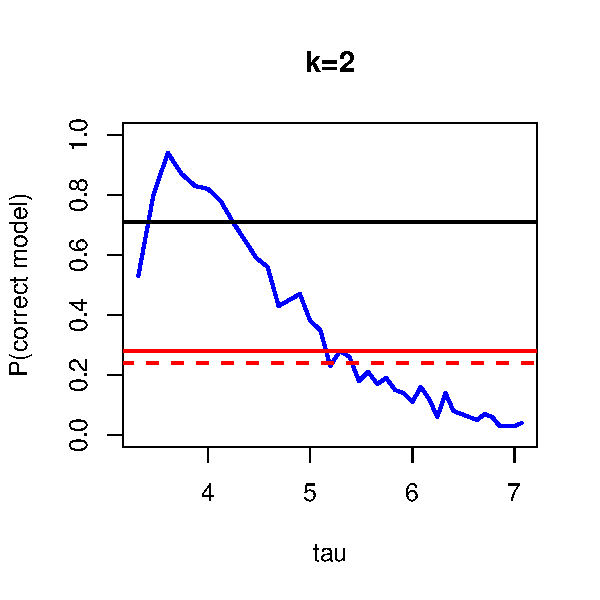
\includegraphics[width=0.32\textwidth]{Chapter-evalue/simplotmoon2}
	& 
		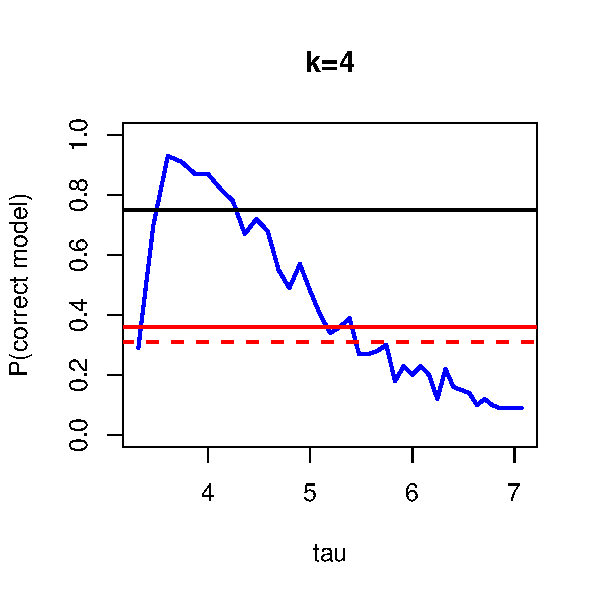
\includegraphics[width=0.32\textwidth]{Chapter-evalue/simplotmoon4} \\
	(a) & (b) \\	
		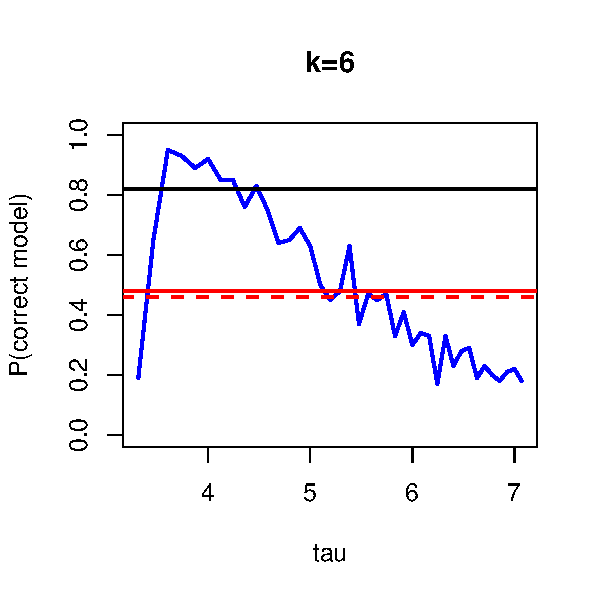
\includegraphics[width=0.32\textwidth]{Chapter-evalue/simplotmoon6}
	& 
		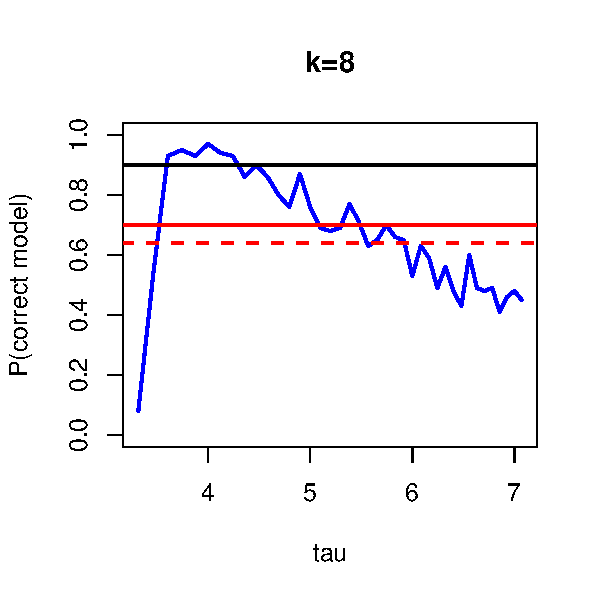
\includegraphics[width=0.32\textwidth]{Chapter-evalue/simplotmoon8} \\
	(c) & (d) \\	
\end{tabular}

\caption{Empirical probabilities of selecting the correct model through moon bootstrap for several levels of sparsity:  The $e$-values method- blue solid, AIC backward deletion- red dotted, AIC all subset- red solid, BIC backward deletion- black dotted, BIC all subset- black solid}
\label{fig:simplotsmoon}

\end{center}
\end{figure}

\begin{figure}
\begin{center}

\begin{tabular}{cc}
		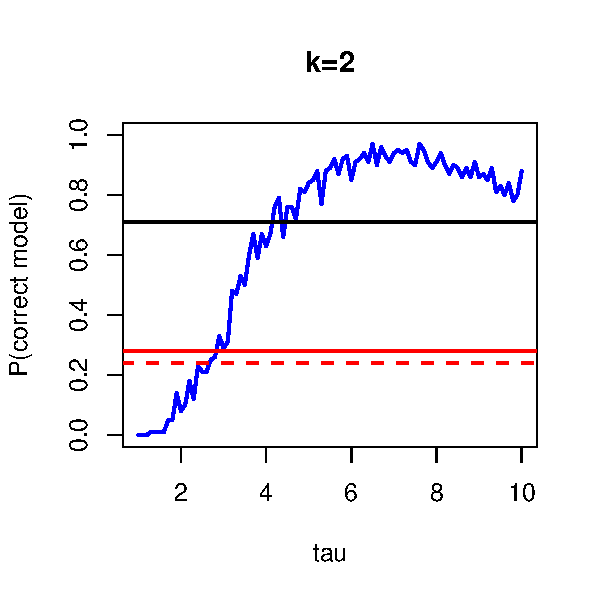
\includegraphics[width=0.32\textwidth]{Chapter-evalue/simplot_gamma2}
	& 
		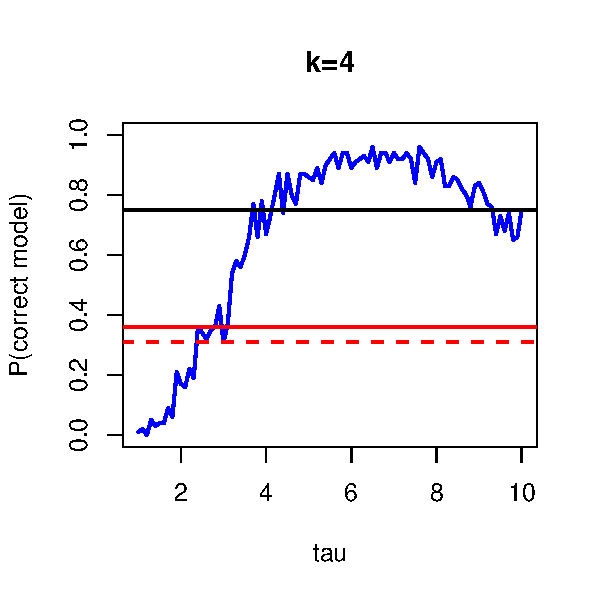
\includegraphics[width=0.32\textwidth]{Chapter-evalue/simplot_gamma4} \\
	(a) & (b) \\	
		\includegraphics[width=0.32\textwidth]{Chapter-evalue/simplot_gamma6}
	& 
		\includegraphics[width=0.32\textwidth]{Chapter-evalue/simplot_gamma8} \\
	(c) & (d) \\	
\end{tabular}

\caption{Empirical probabilities of selecting the correct model through gamma bootstrap for several levels of sparsity:  The $e$-values method- blue solid, AIC backward deletion- red dotted, AIC all subset- red solid, BIC backward deletion- black dotted, BIC all subset- black solid}
\label{fig:simplotsgamma}

\end{center}
\end{figure}

\begin{figure}
\begin{center}

\begin{tabular}{cc}
		\includegraphics[width=0.32\textwidth]{Chapter-evalue/simplot2}
	& 
		\includegraphics[width=0.32\textwidth]{Chapter-evalue/simplot4} \\
	(a) & (b) \\	
		\includegraphics[width=0.32\textwidth]{Chapter-evalue/simplot6}
	& 
		\includegraphics[width=0.32\textwidth]{Chapter-evalue/simplot8} \\
	(c) & (d) \\	
\end{tabular}

\caption{Empirical probabilities of selecting the correct model through wild bootstrap for several levels of sparsity:  The $e$-values method- blue solid, AIC backward deletion- red dotted, AIC all subset- red solid, BIC backward deletion- black dotted, BIC all subset- black solid}
\label{fig:simplotswild}

\end{center}
\end{figure}

We use the backward deletion and all-subset regression search strategies while using AIC and BIC as the model selection criterion. We use the leaps-and-bound algorithm, implemented in the {\texttt{R}} package \texttt{leaps}, for all-subset search. We display the results of this study in \ref{fig:simplotsmoon} for the moon bootstrap, in \ref{fig:simplotsgamma} for the gamma bootstrap and \ref{fig:simplotswild} for a wild bootstrap \citep{Mammen93} version of the linear regression equivalent of \ref{equation:LMMBootEqn} with i.i.d. $N(0,1)$ weights. In all three methods, and for all of $k \in \{2, 4, 6, 8 \}$ the proposed $e$-value based method performs better than AIC or BIC, as long as $\tau_{n}^{2}$ is not too small or too large. This is entirely as expected. The parametric wild bootstrap procedure has the best performance among the three, giving almost perfect detection for even very large values of $\tau_n$.
%Also interestingly, unlike the AIC or BIC, the proposed {\textit{e-value}}-based 
%procedure has the same level of accuracy in detecting the correct model regardless 
%of the amount of sparsity in $\bfbeta$. 
We experimented with other choices of $n, p, R_{1}, R_{2}$, and it seems considering $\tau \in (4, 8)$ 
in this problem ensures exact minimal adequate model selection with high chance, and typically better performance than BIC in this regard. As long as $R$ and $R_{1}$ are of the order of a few hundreds or higher, the variation from the resampling Monte Carlo step seems ignorable.

\subsection{Model selection in the presence of random effects}
Here we use the repeated measures simulation setup from \cite{PengLu12}, which has 9 fixed effects and 4 random effects, with true $\bfbeta = (0,1,1,0,0,0,0,0,0)$ and random effect covariance matrix:
%
\begin{align*}
D = \left(
	\begin{tabular}{cccc}
		9 & ~ & ~ & ~\\
		4.8 & 4 & ~ & ~\\
		0.6 & 1 & 1 & ~\\
		0 & 0 & 0 & 0\\
	\end{tabular}
	\right)
\end{align*}	
%
The error variance $\sigma^2$ is set at 1. The goal is to select the covariates of the fixed effect, thus essentially identify the covariates corresponding to the entries where $\bfbeta$ is non-zero. We use two scenarios for our study: one where the number of subjects considered is $m = 30$,  and the number of observations per subject is $n_i = 5$, and another with 60 subjects and 10 observations per subject.

%The model for the $i^\text{th}$ subject can be written as:
%%
%$$ \bfy_i = X_i \bfbeta + \bfepsilon_i $$
%%
%where $\bfepsilon_i \sim \mathcal N_{n_i} ({\bf 0}, \sigma^2 I + Z_i D Z_i^T)$. We use wild bootstrap on these residuals, so that the bootstrap equivalent of the response will be $\bfy_i^b = X_i \hat\bfbeta_{n,\text{LMM}} + u_{ib} (\bfy_i - X_i \hat\bfbeta_{n,\text{LMM}})$; with $u_{ib} \sim N(0, \tau^2)$. We take the bootstrap standard deviation $\tau = 1,2,...,8$, and determine the accuracy of our method by four measures: 

We consider $\tau \in \{1, \ldots, 15 \}$ here, and use the approximation in \ref{equation:LMMBootEqn} to calculate the bootstrapped coefficients. We consider multiple characteristics of the model that obtains the highest $e$-value, including the number of parameters it involves, the proportion of times the minimal adequate model is 
obtained, the proportion of times a zero-valued (non-zero-valued) element of beta was identified as non-zero (zero), that is, the proportion of false positives (negatives), and so on.   

In the method proposed by \cite{PengLu12}, the tuning parameter can be selected using several different criteria. We present the false positive percentage (FPR\%), false negative percentage (FNR\%) and model sizes corresponding to 
four such criteria. Our results are presented in  \ref{table:simtable1}. It can be seem the $e$-value based method handsomely outperforms the  method proposed by \cite{PengLu12}, especially in smaller sample sizes, as long as $\tau \geq 4$. 

\begin{table}[t]
	\centering
	\begin{scriptsize}
   \begin{tabular}{ll|lll|lll}
    \hline
    Method      & Tuning     & FPR\% & FNR\% & Model size & FPR\% & FNR\% & Model size \\ \cline{3-8}
    ~ & ~ & \multicolumn{3}{l|}{$n_i=5,m=30$} & \multicolumn{3}{l}{$n_i=10,m=60$}\\ \hline
  $e$-value based       & $\tau=1$      & 59.9     & 0.0   & 5.61       & 44.3     & 0.0   & 4.43       \\
    ~      & $\tau=2$      & 33.0     & 0.0   & 3.45       & 15.5     & 0.0   & 2.54       \\
    ~      & $\tau=3$      & 15.9     & 0.0   & 2.59       & 5.2      & 0.0   & 2.17       \\
    ~      & $\tau=4$      & 8.0      & 0.0   & 2.28       & 2.8      & 0.0   & 2.09       \\
    ~      & $\tau=5$      & 5.2     & 0.0   & 2.18       & 2.0   & 0.0   & 2.06       \\
    ~      & $\tau=6$      & 2.7     & 0.0   & 2.09       & 0.7   & 0.0   & 2.02       \\
    ~      & $\tau=7$      & 2.2   & 0.0   & 2.07       & 0.3   & 0.0   & 2.01       \\
    ~      & $\tau=8$      & 1.5   & 0.0   & 2.05       & 0.3   & 0.0   & 2.01       \\
    ~      & $\tau=9$      & 1.0   & 0.0   & 2.03       & 0.3   & 0.0   & 2.01       \\
    ~      & $\tau=10$      & 0.7   & 0.0   & 2.02       & 0.3   & 0.0   & 2.01       \\
    ~      & $\tau=12$      & 0.7   & 0.0   & 2.02       & 0.0   & 0.0   & 2.00       \\
    ~      & $\tau=15$      & 0.7   & 0.0   & 2.02       & 0.0   & 0.0   & 2.00       \\
     \hline
    \cite{PengLu12} & BIC    & 21.5  & 9.9   & 2.26       & 1.5   & 1.9   & 2.10       \\
    ~      & AIC    & 17    & 11.0  & 2.43       & 1.5   & 3.3   & 2.20       \\
    ~      & GCV    & 20.5  & 6     & 2.30       & 1.5   & 3     & 2.18       \\
    ~      & $\sqrt{\log n/n}$ & 21    & 15.6  & 2.67       & 1.5   & 4.1   & 2.26       \\ \hline
    \end{tabular}
    \caption{Comparison between our method and that proposed by \cite{PengLu12} through average false positive percentage, false negative percentage and model size}
    \label{table:simtable1}
    \end{scriptsize}
\end{table}
%
\begin{table}[t]
	\centering
	\begin{scriptsize}
    \begin{tabular}{llll}
    \hline
    Method          & ~ & Setting 1 & Setting 2 \\ \hline
    $e$-value based     & $\tau=1$ & 3         & 14       \\
    ~               & $\tau=2$ & 30      & 60        \\
    ~               & $\tau=3$ & 61        & 86      \\
    ~               & $\tau=4$ & 79        & 92      \\
    ~               & $\tau=5$ & 87        & 94       \\
    ~               & $\tau=6$ & 93      & 98       \\
    ~               & $\tau=7$ & 94       & 99       \\
    ~               & $\tau=8$ & 96       & 99       \\
    ~               & $\tau=9$ & 97       & 99       \\
    ~               & $\tau=10$ & 98       & 99       \\
    ~               & $\tau=12$ & 98       & 100       \\
    ~               & $\tau=15$ & 98       & 100       \\\hline
    \cite{BondellKrishnaGhosh10} & ~ & 73        & 83        \\
    \cite{PengLu12}         & ~ & 49        & 86        \\
    \cite{FanLi12}           & ~ & 90        & 100       \\ \hline
    \end{tabular}
    \caption{Comparison of our method and three sparsity-based methods of mixed effect model selection through accuracy of selecting correct fixed effects}
	\label{table:simtable2MS}
    \end{scriptsize}
\end{table}

We also compare the percentages of times the correct model was identified, and these results are presented in \ref{table:simtable2MS}, along with the corresponding results from two other papers. The proposed $e$-value based procedure performs best here for $\tau \geq 6$ for the smaller sample setting, and for $\tau\geq 12$ for larger sample setting. 


\section{Real data example}
\label{sec:regression-sec6}

\begin{figure}
%\captionsetup{justification=centering, font=footnotesize}
\begin{center}
\includegraphics[width=.8\textwidth]{Chapter-regression/cropped_gene_heatmap1}

\caption{Estimated effects of different pathway genes on the activity of genes in Mevalonate and Non-mevalonate pathways (left and right of vertical line) in \textit{A. thaliana}}
\label{fig:coeffplots}
\end{center}
\end{figure}

\begin{table}[h]
\centering
\begin{footnotesize}
\begin{tabular}{rll}
  \hline
Coeff & Gene & Pathway \\ 
  \hline
0.18 & DPPS2 & Phytosterol biosynthesis \\ 
0.14 & DPPS2 & Carotenoid biosynthesis \\ 
0.14 & DPPS2 & Flavonoid metabolism \\ 
0.11 & DPPS2 & Calvin cycle \\ 
0.11 & PPDS2mt & Phytosterol biosynthesis \\ 
0.10 & GGPPS3 & Cytokinin biosynthesis \\ 
0.10 & PPDS1 & Phytosterol biosynthesis \\ 
0.09 & DPPS3 & Flavonoid metabolism \\ 
0.09 & DPPS3 & Ubiquinone biosynthesis \\ 
0.09 & GGPPS9 & Ubiquinone biosynthesis \\ 
\hline
\end{tabular}
\caption{Top 10 gene-pathway connections in {\it A. thaliana} data found by LARN}
\label{table:coefftable}
\end{footnotesize}
\end{table}

We apply the LARN algorithm on a microarray dataset containing expression of several genes in the flowering plant \textit{Arabidopsis thaliana} \citep{WilleEtal04}. In this dataset, gene expressions are collected from $n=118$ samples, which are plants grown under different experimental conditions. We take the expressions of $q=40$ genes in two pathways for biosynthesis of isoprenoid compounds, which are key compounds affecting plant metabolism as our multiple responses. Expressions of 795 other genes corresponding to 56 other pathways are taken as predictors.

Our objective here is to find out the extent of crosstalk between isoprenoid pathway genes and those in the other pathways. We apply LARN, as well as the two methods mentioned before, on the data and evaluate them based on predictive accuracy of 100 random splits with 90 training samples. All three methods have similar mean squared prediction error (MSPE) (LARN and GL-t have MSPE 0.45 and SGL has 0.44), but LARN produces more sparse solutions on average: the mean proportion of non-zero elements in the coefficient matrix are 0.15, 0.21 and 0.29 for LARN, GL-t and SGL, respectively. Focusing on the coefficient matrix estimated by LARN, we summarize the 10 largest coefficients (in absolute values) in \ref{table:coefftable}. We also visualize coefficients corresponding to genes in the 6 pathways in the table through a heatmap in  \ref{fig:coeffplots}.

All of the four largest coefficients correspond to interactions of one gene, DPPS2, with four different pathways. Two of these pathways, Carotenoid and Phytosterol, directly use products from the isoprenoid pathways, and their connections with DPPS2 had been detected in \cite{WilleEtal04}. The large Calvin Cycle-DPPS2 coefficient reveals that compounds synthesized in Carotenoid and Phytosterol pathways get used in Calvin Cycle. 
In the heatmap, Carotenoid biosynthesis seems to be connected mostly to the non-mevalonate pathway genes (right of the vertical line), while the activities of genes in Cytokinin and Ubiquinone synthesis pathways seem to be connected with those in the mevalonate pathway. These are consistent with the findings of \cite{WilleEtal04}, \cite{FrebortEtal11} and \cite{Disch98}, respectively.

\section{Conclusion}

In this chapter we propose a class of nonconvex penalty functions, based on the idea of inverting data depths, for performing support union recovery in multitask linear regression. Although several nonconvex penalties exist in the literature, the strength of our penalization scheme lies in the significant scope of inference procedures that can rise from the choice of the reference distribution $F$. Here we consider a simplified reference distribution and provide asymptotic oracle results that ensure recovery of the non-zero row support in the coefficient matrix. We also show that a simple post-estimation thresholding recovers non-zero elements within non-zero rows of the estimated coefficient matrix with good accuracy. Although our method shares the weakness of all nonconvex penalties: small signals may go undetected or can be estimated in a biased fashion, the flexibility in choosing $F$ provides enough motivation to fine tune similar penalization schemes. Our immediate plans for future studies include extending this specific setup to generalized linear models, dimensional asymptotics assuming the data dimension $p$ to be a function of sample size $n$, as well as exploring the use of more efficient algorithms for calculating the sparse solutions, e.g. proximal gradient descent or Concave-Convex algorithms \citep{WangKimLi13}.

\section{Proofs}
\label{section:regression-sec8}

\begin{proof}[Proof of theorem \ref{Thm:OracleThm}]

We shall prove a small lemma before going into the actual proof.

\begin{Lemma}\label{Lemma:OracleThmLemma}
For matrices $\bfK \in \mathbb R^{l \times k}, \bfL \in \mathbb R^{l \times m}, \bfM \in \mathbb R^{m \times k}$,
%
$$
\Tr (\bfK^T \bfL \bfM) = {\ve}^T (\bfK) (\bfI_k \otimes \bfL ) \ve (\bfM)
$$
%
\end{Lemma}

\begin{proof}[Proof of lemma \ref{Lemma:OracleThmLemma}]
From the property of Kronecker products, $(\bfI_k \otimes \bfL) \ve(\bfM) = \ve (\bfL\bfM)$. The lemma follows since $\Tr (\bfK^T \bfL \bfM) = \ve^T (\bfK) \ve(\bfL\bfM)$.
\end{proof}

Now, suppose $\bfB = \bfB_0 + \bfU/\sqrt n$, for some $\bfU \in \mathbb R^{p \times q}$, so that our objective function takes the form
%
\begin{eqnarray}\label{eqn:OracleThmEqn1}
T_n (\bfU) &=& \Tr \left[ \left( \bfY - \bfX\bfB_0 - \frac{1}{\sqrt n}\bfX\bfU \right)^T \left( \bfY - \bfX\bfB_0 - \frac{1}{\sqrt n}\bfX\bfU \right)\right] \notag\\
&& + \lambda_n \sum_{j=1}^p p'_F ( r_j^*) \left\| \bfb_{0j} + \frac{\bfu_j}{\sqrt n} \right\|_2 \notag\\
\Rightarrow T_n (\bfU) - T_n ({\bf 0}_{p \times q}) &=& \Tr \left[ \frac{1}{n} \bfU^T \bfX^T \bfX \bfU - \frac{2}{\sqrt n} \bfE^T \bfX\bfU\right] \notag\\
&& + \frac{\lambda_n}{\sqrt n} \sum_{j=1}^p p'_F ( r_j^*) \left( \| \sqrt n\bfb_{0j} + \bfu_j \|_2 - \| \sqrt n\bfb_{0j} \|_2 \right)  \notag\\
&=& \Tr (\bfV_1 + \bfV_2) + V_3
\end{eqnarray}

Since $\bfX^T\bfX/n \rightarrow \bfC$ by assumption, we have $\Tr(\bfV_1) \rightarrow \ve^T (\bfU)(\bfI_q \otimes \bfC) \ve(\bfU)$ using lemma \ref{Lemma:OracleThmLemma}. Using the lemma we also get
%
$$
\Tr(\bfV_2) = \frac{2}{\sqrt n} {\ve}^T(\bfE) (\bfI_q \otimes \bfX) \ve (\bfU)
$$
%
Now $\ve(\bfE) \sim \mathcal N_{nq} ({\bf 0}_n, \bfSigma \otimes \bfI_q)$, so that $(\bfI_q \otimes \bfX^T) \ve(\bfE)/\sqrt n \leadsto \bfW \equiv \mathcal N_{pq} ({\bf 0}_{pq}, \bfSigma \otimes \bfC)$ using properties of Kronecker products and Slutsky's theorem.

Let us look at $V_3$ now. Denote by $V_{3j}$ the $j$-th summand of $V_3$. Now there are two scenarios. Firstly, when $\bfb_{0j} \neq {\bf 0}_q$, we have $p'_F ( r_j^*) \stackrel{P}{\rightarrow} p'_F ( r_{0j})$. Since $\lambda_n / \sqrt n \rightarrow 0$, this implies $V_{3j} \stackrel{P}{\rightarrow} 0$ for any fixed $\bfu_j$. Secondly, when $\bfb_{0j} = {\bf 0}_q$, we have
%
$$
V_{3j} = \lambda_n n^{(s-1)/2}. (\sqrt n r^*_j )^{-s}.\frac{ p'_F ( r_j^*) \| \bfu_j \|_2 }{ (r^*_j) ^{-s}}
$$
%
We now have $\bfb^*_j = O_p(1/\sqrt n)$, and also each term of the gradient vector is $O ((r^*_j)^{-s})$ by assumption. Thus $V_{3j} = O_P( \lambda_n n^{(s-1)/2} \| \bfu_j \|_2)$. By assumption, $\lambda_n n^{(s-1)/2} \rightarrow \infty$ as $n \rightarrow \infty$, so $V_{3j} \stackrel{P}{\rightarrow} \infty$ unless $\bfu_j = {\bf 0}_q$, in which case $V_{3j} = 0$.

Accumulating all the terms and putting them into \ref{eqn:OracleThmEqn1} we see that
%
\begin{equation}
T_n(\bfU) - T_n({\bf 0}_{p \times q}) \leadsto
\begin{cases}
\ve^T (\bfU_1) [ (\bfI_q \otimes \bfC_{11}) \ve(\bfU_1) - 2 \bfW_1 ] & \text{if } \bfU_0 = {\bf 0}_{(p-p_1)q}\\
\infty & \text{otherwise}
\end{cases}
\end{equation}
where rows of $\bfU$ are partitioned into $\bfU_1$ and $\bfU_0$ according to the zero and non-zero rows of $\bfB_0$, respectively, and the random variable $\bfW$ is partitioned into $\bfW_1$ and $\bfW_0$ according to zero and non-zero \textit{elements} of $\ve (\bfB_0)$. Applying epiconvergence results of \cite{Geyer94} and \cite{KnightFu00} we now have
%
\begin{eqnarray}
\ve(\hat\bfU_{1n}) &\leadsto & (\bfI_q \otimes \bfC_{11}^{-1}) \bfW_1\label{eqn:OracleThmProofEqn2}\\
\ve(\hat\bfU_{0n}) &\leadsto & {\bf 0}_{(p-p_1)q}\label{eqn:OracleThmProofEqn3}
\end{eqnarray}
%
where $\hat\bfU_n = (\hat\bfU_{1n}^T, \hat\bfU_{0n}^T)^T := \argmin_\bfU T_n (\bfU)$.

The second part of the theorem, i.e. asymptotic normality of $\sqrt n (\ve (\hat \bfB_{1n}) - \ve(\hat\bfB_{1n})) = \hat\bfU_{1n}$ follows directly from \ref{eqn:OracleThmProofEqn2}. It is now sufficient to show that $P( \hat\bfb_j^{(1)} \neq {\bf 0}_q | \bfb_{0j} = {\bf 0}_q) \rightarrow 0$ to prove the oracle consistency part. For this notice that KKT conditions of the optimization problem for the one-step estimate indicate
%
\begin{equation}
2 \bfx_j^T (\bfY - \bfX \hat\bfB^{(1)}) = - \lambda_n p'_F (r_j^*) \frac{\bfb_j^{(1)}}{r_j^{(1)}} \quad\Rightarrow\quad \frac{2 \bfx_j^T (\bfY - \bfX \hat\bfB^{(1)})}{\sqrt n} = - \frac{\lambda_n p'_F (r_j^*)}{\sqrt n}. \frac{\bfb_j^{(1)}}{r_j^{(1)}}
\end{equation}
%
for any $1 \leq j \leq p$ such that $\hat\bfb_j^{(1)} \neq {\bf 0}_q$. Since $p'_F(r_j^*) = D^-( (r_j^*)^{-s}) = O_P ( \| (\bfb_{0j} + 1/\sqrt n \|^{-s})$ and $\lambda_n n^{(s-1)/2} \rightarrow \infty$, the right hand side goes to $-\infty$ in probability if $\bfb_{0j} = {\bf 0}_q$. As for the left-hand side, it can be written as
%
$$ \frac{2 \bfx_j^T (\bfY - \bfX \hat\bfB^{(1)})}{\sqrt n} = \frac{2 \bfx_j^T \bfX .\sqrt n (\bfB_0 - \hat\bfB^{(1)})}{n} + \frac{2 \bfx_j^T \bfE}{\sqrt n} = \frac{2 \bfx_j^T \bfX \hat\bfU_n}{n} + \frac{2 \bfx_j^T \bfE}{\sqrt n}
$$
%
Our previous derivations show that vectorized versions of $\hat\bfU_n$ and $\bfE$ have asymptotic and exact multivariate normal distributions, respectively. Hence
%
$$
\BP \left[ \hat\bfb_j^{(1)} \neq {\bf 0}_q | \bfb_{0j} = {\bf 0}_q \right] \leq P \left[ 2 \bfx_j^T (\bfY - \bfX \hat\bfB^{(1)} ) = - \lambda_n p'_F (r_j^*) \frac{\bfb_j^{(1)}}{r_j^{(1)}} \right] \rightarrow 0
$$
\end{proof}

\begin{proof}[Proof of theorem \ref{Thm:RowSupportThm}]
See the proof of corollary 2 of \cite{ObozinskiEtal11}in Appendix A therein. Our proof follows the same steps, only replacing $\bfSigma_{SS}$ with $\bfSigma \otimes \bfC_{11}$.

\end{proof}

\begin{proof}[Proof of Lemma \ref{thm:minimaxThm}]
We broadly proceed in a similar fashion as the proof of Theorem 3 in \cite{Zou06}. As a first step, we decompose the mean squared error:
%
\begin{eqnarray*}
E[ \hat\theta(F,\lambda) - \theta]^2 &=& E[ \hat\theta(F,\lambda) - z]^2 + E(z - \theta)^2 + 2 E [\hat\theta(F,\lambda) (z-\theta)] - 2E [z(z-\theta)]\\
&=& E[ \hat\theta(F,\lambda) - z]^2 + E \left[ \frac{d\hat\theta(F,\lambda)}{dz}\right] - 1
\end{eqnarray*}
%
by applying Stein's lemma \citep{Stein81}. We now use Theorem 1 of \cite{AntoniadisFan01} to approximate $\hat\theta(F,\lambda)$ in terms of $y$ only. By part 2 of the theorem,
%
\begin{equation}
\hat\theta(F,\lambda) = \begin{cases}
0 \quad & \text{if } |z| \leq \lambda p_0(F)\\
z - \text{sign}(z). \lambda D^-_1(\hat\theta(F,\lambda), F) & \text{if }|z| > \lambda p_0(F)
\end{cases}
\end{equation}
%
Moreover, applying part 5 of the theorem,
%
\begin{equation}
\hat\theta(F,\lambda) = z - \text{sign}(z).\lambda D^-_1(z, F) + o(D^-_1(z, F))
\end{equation}
%
for $|z| > \lambda p_0(F)$. Thus we get
%
\begin{equation}
[ \hat\theta(F,\lambda) - z]^2 = \begin{cases}
z^2 & \text{if } |z| \leq \lambda p_0(F)\\
\lambda^2 D^-_1(z,F)^2 + k_1(|z|) & \text{if } |z| > \lambda p_0(F)
\end{cases}
\end{equation}
%
and
%
\begin{equation}
\frac{d\hat\theta(F,\lambda)}{dz} = \begin{cases}
0 & \text{if } |z| \leq \lambda p_0(F)\\
1 +  \lambda D^-_2(z,F) + k_1'(|z|) & \text{if } |z| > \lambda p_0(F)
\end{cases}
\end{equation}
%
where $k_1(|z|) = o(|z|)$, and $D^-_2(z,F) = d^2D^-(z,F)/dz^2$. Thus
%
\begin{eqnarray}\label{eqn:MinimaxProofEqn1}
E [ \hat\theta(F,\lambda) - \theta]^2 &=& E [z^2 \BI_{|z| \leq \lambda p_0(F)}] + E \left[ \left(\lambda^2 D^-_1(|z|, F)^2 + 2 \lambda D^-_2(|z|,F) + 2 + \right.\right. \notag\\
&& \left.\left. k_1(|z|) + k_1'(|z|) \right) \BI_{|z| > \lambda p_0(F)} \right] - 1
\end{eqnarray}
%
Now
%
\begin{eqnarray*}
k_1(|z|) &=& \lambda^2 \left[ D^-_1(z,F)^2 - D^-_1(\hat\theta(F,\lambda), F)^2 \right] \quad \leq \quad \lambda^2 c_1^2, \text{ and}\\
| k_1'(|z|) | &=& \lambda \left| D^-_2(z,F) - \frac{d D^-_1(\hat\theta(F,\lambda), F)}{dz} \right| \quad \leq \quad 2\lambda c_2
\end{eqnarray*}
%
Substituting these in \ref{eqn:MinimaxProofEqn1} above we get
%
\begin{eqnarray}\label{eqn:MinimaxProofEqn2}
E [ \hat\theta(F,\lambda) - \theta]^2 & \leq & \lambda^2 p_0(F)^2 P [|z| \leq \lambda p_0(F)] + E \left[ \left(\lambda^2 f^2(|z|) + 2 \lambda D^-_2(z, F) \right) BI_{|z| > \lambda p_0(F)} \right] \notag\\
&& + \lambda^2 c_1^2 + 2\lambda c_2 + 1 \notag\\
& \leq & 2\lambda^2 c_1^2 + 4 \lambda c_2 + 1 \notag\\
& \leq & 4\lambda^2 c_1^2 + 8 \lambda c_2 + 1
\end{eqnarray}
%

Adding and subtracting $z^2 \BI_{|z| > \lambda p_0(F)}$ to the first and second summands of \ref{eqn:MinimaxProofEqn1} above, we also have
%
\begin{eqnarray}
E [ \hat\theta(F,\lambda) - \theta]^2 &=& Ez^2 + E \left[ \left(\lambda^2 D^-_1(z,F)^2 + 2 \lambda D^-_2(z,F) + 2 - y^2 + \lambda^2 c_1^2 \right.\right. \notag\\
& & \left.\left. + 2\lambda c_2 \right) \BI_{|z| > \lambda p_0(F)} \right] - 1\notag\\
& \leq & (2 \lambda^2 c_1^2 + 4 \lambda c_2) P [ |z| > \lambda p_0(F) ] + \theta^2
\end{eqnarray}
%
Following \cite{Zou06}, $P[|z| > \lambda p_0(F)] \leq 2q (\lambda p_0(F)) + 2\theta^2$, with $q(x) = \exp[-x^2/2]/(\sqrt{2\pi} x)$. Thus
%
\begin{eqnarray}
E [ \hat\theta(F,\lambda) - \theta]^2 &\leq & 2 (2 \lambda^2 c_1^2 + 4 \lambda c_2) [q (\lambda p_0(F)) + \theta^2] + \theta^2\notag\\
& \leq & (4\lambda^2 c_1^2 + 8 \lambda c_2 + 1)[q (\lambda p_0(F)) + \theta^2] 
\end{eqnarray}
%
Combining this with \ref{eqn:MinimaxProofEqn2} we get
%
\begin{equation}
E [ \hat\theta(F,\lambda) - \theta]^2 \leq [ 4(\lambda c_1 + 1)^2 - 3][q (\lambda p_0(F)) + \min(\theta^2,1)] 
\end{equation}
%
assuming without loss of generality that $c_1 \geq c_2$. Since $R(\text{ideal}) = \min(\theta^2,1)$ and $q(x) \leq (\sqrt{2\pi} x)^{-1} < 1/x$, we have the needed.
\end{proof}


\chapter{Future Work}
% Conclusion

\section{Characterization of depth in general normed spaces}
As mentioned in the beginning of this thesis, a normed space and a probability measure in it are the only requirements to motivate the definition of a depth-like quantity. For example consider the Wasserstein metric on a Radon space $(M,d)$, i.e. a metric space for which every probability measure defined on its borel subsets is inner regular. For any two measures $\mu$ and $\nu$ that values in this space and have finite $p$-th moment for some $p \in \BN$, the $p$-th Wasserstein distance is defined as:
%
\begin{align}\label{eqn:WpEqn}
W_p (\mu, \nu) = \left[ \inf_{ G \in \mathbb G (\mu, \nu)} \int_{M \times M} d(x, y)^p dG(x,y) \right]^{1/p}
\end{align}
%
where $\mathbb G (\mu, \nu)$ is the collection of all `couplings' of the measures $\mu$ and $\nu$: a coupling being a probability measure in $M \times M$ with $\mu$ and $\nu$ at its corresponding marginals.

Now just consider $\mu = \delta_{ x_0}$ i.e. the degenerate distribution at some $x_0 \in M$. In that case the infimum in \ref{eqn:WpEqn} shall be taken over all possible \textit{conditional couplings} of $\nu$ and $x_0$, i.e. random vectors in $M \times M$ such that $x_0$ in the first part can come from any distribution, but is fixed at $x_0$, while the marginal in second part is $\nu$. It is easy to show that
%
$$
W_p ( \delta_{ x_0}, \nu) = \left[ \int d(x_0, x)^p d\nu (x) \right]^{1/p}
$$
%
Here we can look at the quantity $W_p (\delta_{ x_0}, \nu)$ as a generalized outlyingness function.

Similar formulations are possible for other distributional distance measures as well. We plan to investigate this idea in future. Some relevant theoretical machinery for this is possibly available in \cite{LeskelaVihola15} and \cite{DedeckerMichel11}.

\section{Future of $e$-values}
In \ref{chapter:evalue-chapter} we only discuss a very specialized implementation of the $e$-values, in statistical model selection. As seen in \ref{sec:TwinSection} of \ref{chapter:appli-chapter}, using other functionals of the evaluation map distribution can give more refined inference that can be tweaked to suit the need for the data-analytic task in hand and inference objectives of the practitioner. We plan to investigate this in future. We know that the concept of using tail probabilities that yields favorable results in \ref{sec:TwinSection} works in practice, but need to formalize this concept, as well as study in detail the contrasting tail behaviors of adequate and inadequate models. Specific implementations of the variable selection technique are also of interest, for example in robust regression through the usage of robust bootstrap \citep{SBVanAelst08, SBZamar02}, or even as a measure of variable importance in machine learning methods like random forest or boosting.

\section{Others}
Reiterating from the conclusions of \ref{chapter:scatter-chapter}, the scope of application for the inverse depth-based rank transformation needs to be investigated. A low-hanging fruit in this respect can be its application in functional data. The generic regularization structure presented in \ref{chapter:regression-chapter}, i.e. \ref{eqn:eqn02} therein, is very interesting. The choice of the reference distribution $F$ represents an initial belief on the correlation structure of responses, and can easily be interpreted as a prior distribution. A study of the methods and modelling algorithms that can possibly arise from such a formulation of bayesian multitask penalized regression is something we want to pursue in future.
% References don't have to be double spaced either
%\setstretch{1.2}
\bibliographystyle{apalike}
\bibliography{introbib,MSbib,climate,fmribib,snpbib,scatterbib,regbib}

\end{document}